\documentclass[11pt,oneside]{book}
\usepackage{fontspec}
\usepackage{xeCJK}
\setmainfont{Latin Modern Roman}
\setCJKmainfont[ItalicFont={Noto Serif CJK JP},BoldItalicFont={Noto Serif CJK JP Bold}]{Noto Serif CJK JP}
\setCJKsansfont{Noto Sans CJK JP}
\setCJKmonofont{Noto Sans Mono CJK JP}
\newfontfamily\proseunicodefont{DejaVu Serif}
\usepackage[margin=1in]{geometry}
\usepackage{microtype}
\usepackage{amsmath,amssymb,amsthm,mathtools,bm}
\usepackage{graphicx}
\usepackage{xcolor}
\usepackage{booktabs}
\usepackage{array}
\usepackage{longtable}
\usepackage{enumitem}
\usepackage{float}
\usepackage{caption}
\usepackage{hyperref}
\usepackage{fancyhdr}
\usepackage{tikz}
\usetikzlibrary{arrows.meta,positioning,calc,decorations.pathmorphing}

\hypersetup{
  colorlinks=true,
  linkcolor=blue!50!black,
  urlcolor=blue!50!black,
  citecolor=blue!50!black
}

\setlength{\parskip}{0.5em}
\setlength{\parindent}{0pt}
\setlist[itemize]{topsep=0.25em,itemsep=0.2em}
\setlist[enumerate]{topsep=0.25em,itemsep=0.2em}
\setlength{\headheight}{40pt}
\numberwithin{equation}{chapter}

\newtheorem{theorem}{定理}[chapter]
\newtheorem{proposition}[theorem]{命題}
\newtheorem{lemma}[theorem]{補題}
\newtheorem{corollary}[theorem]{系}
\theoremstyle{definition}
\newtheorem{definition}[theorem]{定義}
\newtheorem{example}[theorem]{例}
\theoremstyle{remark}
\newtheorem{remark}[theorem]{注意}

\providecommand{\ket}[1]{\left\lvert#1\right\rangle}
\providecommand{\bra}[1]{\left\langle#1\right\rvert}
\providecommand{\braket}[2]{\left\langle#1\,\middle|\,#2\right\rangle}
\providecommand{\expect}[1]{\left\langle#1\right\rangle}
\newcommand{\lectureoverview}[1]{\paragraph{概観。} #1}

\makeatletter
\newcommand{\course@headerfont}{\normalfont\small\itshape}
\newcommand{\course@pagefont}{\normalfont\small}
\newcommand{\course@headerraise}{14pt}
\newlength{\course@headerboxheight}
\setlength{\course@headerboxheight}{\dimexpr\headheight-\course@headerraise-9pt\relax}
\newcommand{\course@leftheadbox}[1]{%
  \raisebox{\course@headerraise}{%
    \parbox[t][\course@headerboxheight][t]{0.82\textwidth}{%
      \raggedright\course@headerfont\strut\MakeUppercase{#1}\strut%
    }%
  }%
}
\newcommand{\course@rightheadbox}[1]{%
  \raisebox{\course@headerraise}{%
    \parbox[t][\course@headerboxheight][t]{0.82\textwidth}{%
      \raggedleft\course@headerfont\strut\MakeUppercase{#1}\strut%
    }%
  }%
}
\renewcommand{\chaptermark}[1]{\markboth{\MakeUppercase{\chaptername\ \thechapter.\ #1}}{}}
\renewcommand{\sectionmark}[1]{\markright{\MakeUppercase{\thesection\hspace{0.4em}#1}}}
\fancyhf{}
\fancyhead[L]{\course@leftheadbox{\leftmark}}
\fancyhead[R]{\course@pagefont\thepage}
\renewcommand{\headrulewidth}{0.5pt}
\pagestyle{fancy}
\fancypagestyle{plain}{%
  \fancyhf{}
  \fancyhead[L]{\course@leftheadbox{\leftmark}}
  \fancyhead[R]{\course@pagefont\thepage}
  \renewcommand{\headrulewidth}{0.5pt}
}
\makeatother

% Video2Book editorial provenance macros
\newenvironment{classroomqa}{%
  \par\medskip\noindent\begin{minipage}{\linewidth}\small\hrule\medskip
}{%
  \medskip\hrule\end{minipage}\par\medskip
}
\newcommand{\audiencequestion}[1]{\noindent\textbf{受講者からの質問。} #1\par\smallskip}
\newcommand{\lecturerresponse}[1]{\noindent\textbf{回答。} #1\par}
\newcommand{\lecturetimestamp}[1]{\footnote{講義時刻： #1.}}
\newcommand{\lectureframe}[1]{\par\smallskip{\centering\footnotesize\itshape 講義映像： #1.\par}}
\newcommand{\editorialnote}[1]{\footnote{編集上の補足： #1}}

\renewcommand{\contentsname}{目次}
\renewcommand{\chaptername}{章}
\renewcommand{\figurename}{図}
\renewcommand{\tablename}{表}
\renewcommand{\proofname}{証明}
\renewcommand{\bibname}{参考文献}
\emergencystretch=2em
\pdfstringdefDisableCommands{\def\proseunicodefont{}}

\geometry{paperwidth=177.6mm,paperheight=252mm,left=16mm,right=16mm,
 top=18mm,bottom=18mm,includeheadfoot,headheight=28pt,headsep=7mm,footskip=9mm}
\usepackage{scrextend}
\changefontsizes[17pt]{12pt}
\raggedbottom
\renewenvironment{classroomqa}{\par\medskip\begingroup}{\par\endgroup\medskip}
\fancyhf{}
\setlength{\headwidth}{\textwidth}
\fancyhead[L]{\parbox{\textwidth}{\raggedright\fontsize{9}{11}\selectfont\nouppercase{\leftmark}}}
\fancyfoot[C]{\small\thepage}
\renewcommand{\headrulewidth}{0.3pt}
\fancypagestyle{plain}{\fancyhf{}\fancyfoot[C]{\small\thepage}\renewcommand{\headrulewidth}{0pt}}

\graphicspath{{../../../generated_course_notes/supplementary/particle_physics_1_basic_concepts/2009_fall/figures/}{../../../generated_course_notes/supplementary/particle_physics_1_basic_concepts/2009_fall/assets/}}
\begin{document}
\frontmatter
\hypersetup{pageanchor=false}
\begin{titlepage}
\thispagestyle{empty}
\begin{tikzpicture}[remember picture,overlay]
  \node[anchor=center,inner sep=0] at (current page.center) {%
    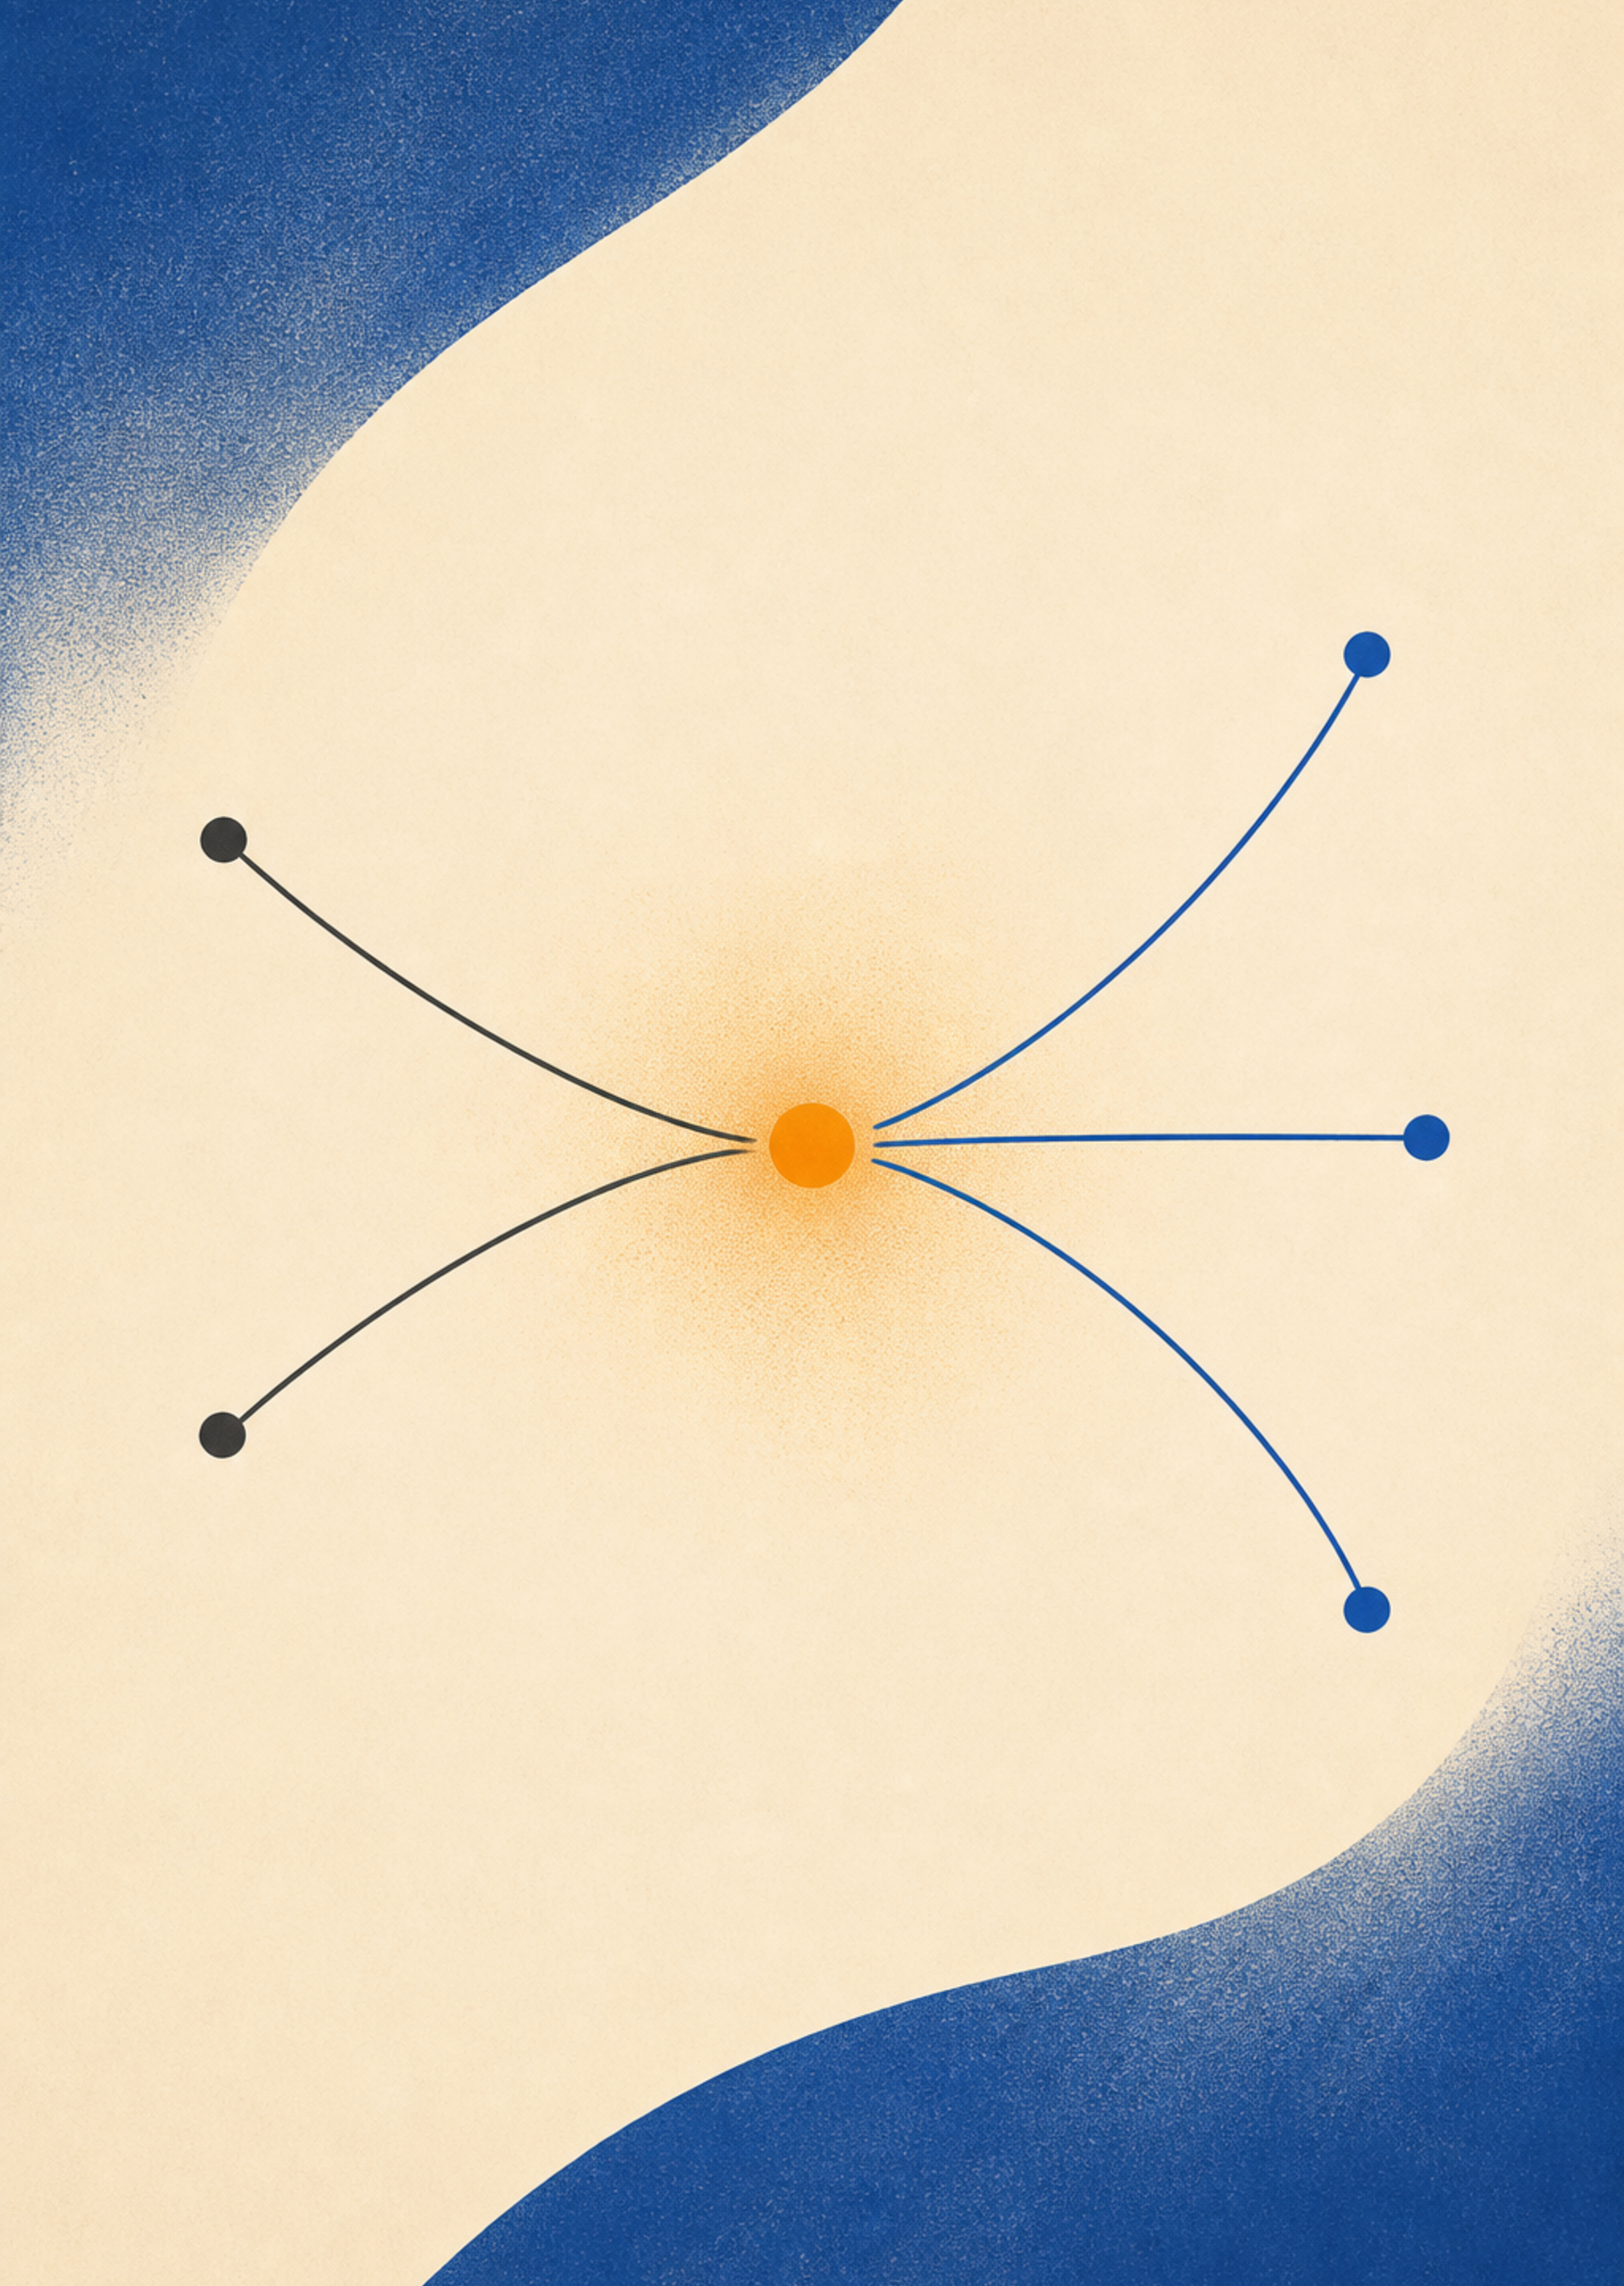
\includegraphics[height=\paperheight,keepaspectratio]{../../../generated_course_notes/supplementary/particle_physics_1_basic_concepts/2009_fall/assets/cover-art.png}%
  };
  \node[
    anchor=north west,
    align=left,
    text width=0.78\paperwidth,
    fill=white,
    fill opacity=0.9,
    rounded corners=8pt,
    inner xsep=10pt,
    inner ysep=8pt
  ] at ([xshift=0.08\paperwidth,yshift=-0.06\paperheight]current page.north west) {%
    {\fontsize{30}{33}\selectfont\bfseries\color{black!88} 素粒子物理学1：基礎概念\\[0.85em]}
    {\large\color{black!72} 日本語版 / 2009 fall}
  };
  \node[
    anchor=south west,
    align=left,
    text width=0.68\paperwidth,
    fill=white,
    fill opacity=0.82,
    text opacity=1,
    rounded corners=6pt,
    inner sep=12pt
  ] at ([xshift=0.08\paperwidth,yshift=0.08\paperheight]current page.south west) {%
    {\normalsize\color{black!78} 原講義：Leonard Susskind\\[0.35em]}
    {\small\color{black!72} 講義補助版：\href{https://lazying.art}{LazyingArt LLC} / \href{https://github.com/lachlanchen/Video2Book}{Video2Book}}
  };
\end{tikzpicture}
\mbox{}
\end{titlepage}
\hypersetup{pageanchor=true}

\clearpage
\chapter*{本ノートについて}
これらの独立に編集された伴走ノートは、Leonard Susskind による講義に基づくものである。これらは機械文字起こし、字幕、および選ばれた黒板画像から再構成され、その後、利用可能な原資料と照合された。これらは Susskind 教授による原著原稿ではなく、同教授による査読や承認も受けていない。

本版は \href{https://lazying.art}{LazyingArt LLC} がオープンソースの \href{https://github.com/lachlanchen/Video2Book}{Video2Book} ワークフローを用いて作成した。機械文字起こしは別途利用可能であり、認識誤りを含む可能性がある。編集上の明確化および自明でない再構成は脚注で示されている。
\clearpage
\tableofcontents
\mainmatter
\chapter{粒子、波、および分解能のエネルギー}

\section{粒子か場か？}

素粒子物理学とは何を扱うのか。粒子---だが、その答えは直ちに古くからの問いを呼び起こす。自然は離散的だろうか。ここで離散的とは、物質が分離した不可分の単位からなるということであり、角が立たないという意味ではない。ギリシア語の\emph{アトム}は不可分を意味するが、現在アトムと呼ばれる物体は分割できる。当面、\emph{粒子}を離散的な単位の総称とする。

対立する描像は連続体である。その場合、物質は分離した断片の集まりではなく、空間を通じて連続的に広がるものである。その自然な言語は場の言語である。場とは位置の関数である。物質の密度は場であり、電場と磁場も場である。後者は荷電粒子がどのように運動するかを決めるが、場それ自体は古典的には空間に連続的に分布するものとして考えられる。

これらの考えの歴史的順序はあまり厳密に押し付けるべきではない。この順序が有用なのは、議論の論理を示すからであり、信頼できる年代順を与えるからではない。粒子の語彙には原子、分子、衝突、局在した物体が含まれ、連続体の語彙には場と連続的に変化する性質が含まれる。どちらの描像が正しいのか。量子力学はどちらも完全に正しいことを妨げるが、どちらも完全に誤りであることも妨げる。

以下の議論は部分的には自己完結的であるが、後の議論では量子力学、古典力学、特殊相対性理論、電磁気学を利用する。当面の問いはもっと単純である。物質が本当に離散的であると人々を最初に納得させたのは何か。

\section{離散的物質の化学的証拠}

少なくともこの論理的な説明では、最初の真剣な証拠は物理学ではなく化学から来た。この区別は人為的である。化学は大部分が原子と分子の物理学である。ドルトンは異なる物質の同数の分子の質量を比較した。試料が同数の分子を含むことを確立すること自体が大きな問題であった。ここでアボガドロの名が登場し、モルはアボガドロ数個の分子である。同じ数の分子を含む試料を比較するだけなら、その数の実際の値は必要なかった。

目覚ましいパターンは、モル質量が水素のモル質量のほぼ整数倍で現れることであった。その倍数は一般に\(3/2\)や\(\pi\)や任意の実数ではなく、整数に近い数であった。例えば炭素-12は、水素が表す質量単位をおよそ12個持つ。これはほぼ同じ質量の反復する構成要素からできていることを強く示唆する。

現代的な説明はこの謎を取り除く。通常の原子には陽子、中性子、電子が含まれている。電子の質量は陽子や中性子のわずか約二千分の一にすぎないため、電子が原子質量に寄与する割合は小さい。陽子と中性子がそのほとんどすべてを担っており、両者の質量の差は一パーセントよりはるかに小さい。通常の水素の原子核は陽子一個であるから、原子や分子の質量は水素程度の核質量のほぼ整数倍となる。この記述はあくまで近似的である。陽子と中性子の質量は同一ではなく、電子もわずかに寄与する。それでもなお、このほぼ整数倍という規則性は離散的な構成要素の存在を明らかにしている。

その後、分子は原子の組み合わせとして理解された。19世紀の化学はおよそ100種類の原子を同定し、それらを元素として整理した。初等的な数え方ではおよそ92種類が天然に存在し、同位体を含めるとさらに区別が増える。周期表は等しいブロックを単純に繰り返すという素朴な意味での周期的ではないが、それらの別個の種を整理した。その段階では、元素それ自体が基本的な構成要素のように見えた。アインシュタインの1905年の仕事は、物質の分子論をはるかに決定的に確立する定量的な方法を与えたが、化学的証拠はすでに原子描像を説得力のあるものにしていた。

19世紀の終わり近くに、この見かけ上の終着点は破綻した。電子が発見され、放射能は元素が基本的であるという描像に収まらない現象を明らかにした。放射能は、後に核物理学と素粒子物理学となる多くの問いを、すでに縮図として内包していた。

\section{放射能と分離されたビーム}

正確な帰属と年代順は不確かである。ベクレルは、放射性物質がたまたま写真乾板の近くにあり、あたかも不可視の放射線がそれを照射したかのように乾板に影響を与えたという観察と暫定的に関連づけられている。かぶった乾板を単に台無しになったものとして扱うのではなく、そこに何が到達したのかを問うこともできた。マリー・キュリーのその後の広範な研究もまたこの歴史に属するが、初期の発見の正確な分担は、この実験的論理には必要ない。

物質を密な鉛ブロックの深部に置き、写真乾板へ向かう細い通路を残す。鉛は密度が高いため有用であり、通路は逃げ出すものをコリメートする。拡散した露光ではなく、乾板には局所的な斑点が現れ、指向性のあるビームを示唆する。この論理的な意味でそれは最初の粒子ビームであるが、この段階ではビームの本性は不明である。

次に、コリメートされた放射を、軌道の平面に垂直な磁場に通す。露光は三つの枝に分かれる。一つは偏向されずに進む。二つは逆向きに曲がり、しかも不等な量だけ曲がる。磁気力は電荷の符号が逆になると向きが逆になるので、逆向きに曲がった枝は逆向きに帯電した放射として振る舞い、直進する枝は中性の放射として振る舞う。\footnote{模式図は、講義動画において00:14:34と00:19:31の間に展開された図を再構成したものである。}

\begin{figure}[h]
\centering
\begin{tikzpicture}[scale=0.92]
\draw[fill=gray!20] (0,-1.55) rectangle (2.1,1.55);
\draw[fill=white,draw=none] (1.02,-0.13) rectangle (2.12,0.13);
\draw[fill=black] (1.02,0) circle (0.07);
\node[below] at (1.02,-0.12) {\small source};
\node[above] at (1.05,1.55) {\small lead};
\foreach \x in {3.0,3.55,4.1}
  \foreach \y in {-0.55,0,0.55}
    \node at (\x,\y) {\(\otimes\)};
\node[above] at (3.55,0.78) {\small \(\mathbf B\) into the page};
\draw[thick] (7,-1.8) -- (7,1.8);
\node[above] at (7,1.8) {\small plate};
\draw[thick,->] (2.1,0) -- (6.85,0);
\draw[thick,->] (2.1,0) .. controls (4.0,0.05) and (5.35,0.40) .. (6.85,0.88);
\draw[thick,->] (2.1,0) .. controls (3.7,-0.08) and (5.0,-0.75) .. (6.85,-1.42);
\node[right] at (7,0.88) {\small \(\alpha\)};
\node[right] at (7,0) {\small \(\gamma\)};
\node[right] at (7,-1.42) {\small \(\beta\)};
\end{tikzpicture}
\caption{横方向の磁場中にあるコリメートされた放射性ビーム。中性成分は偏向されず、逆向きに帯電した成分は不等な量だけ逆向きに曲がる。}
\end{figure}

三つの成分はアルファ、ベータ、ガンマと名づけられた。現代的な用語では、
\begin{equation}
\begin{aligned}
\beta\text{-radiation} &= \text{electrons},\\
\alpha\text{-radiation} &= \text{helium nuclei},\\
\gamma\text{-radiation} &= \text{photons}.
\end{aligned}
\end{equation}
アルファ粒子は二つの陽子と二つの中性子を含み、その質量数四を説明する。ドルトンの近似的な整数の系列では、ヘリウムはしたがって番号四を占めることになる。すなわち四つの水素スケールの核単位である。ベータ線は、陰極線実験からすでに知られていた負に帯電した電子である。ガンマ線は電荷を運ばない。

十分に希薄な線源と、個々の到来を分解できる検出器を用いれば、連続的に見える露光は別々の事象の列になる。ブリップ、ブリップ、ブリップ。同じことはベータ線、アルファ線、ガンマ線についても行える。ガイガー計数管は、最も初期の装置がまさにその領域で操作されていたかどうかにかかわらず、正しい描像を与える。各成分は離散的な束として到来する。ガンマは依然として謎である。それは中性であるのに、一度に一つの事象として検出される。ガンマ線は非常に高エネルギーの光であり、プランク、とりわけアインシュタインは光を量子と結びつけた。しかし、その結論に立ち向かう前に、光が波であるという古典的な証拠を真剣に受け止めなければならない。

\section{光の古典的波動性}

古典的には、光は連続性の最も強い例であった。それは連続的な波として伝播する電場と磁場からなる。ニュートンは粒子説を好んだが、波動の実験がそれを退けた。電荷を揺さぶると電磁放射が生じる。巨視的なアンテナは電波、マイクロ波、赤外線、可視光、または紫外線を放出でき、原子内を回る電荷もまたアンテナである。放出された放射は写真乾板を露光させうる。

単一の開口は波動的振る舞いの最初の兆候を与える。もし光が弾丸の流れであれば、小さな開口は鋭くコリメートされた斑点を作ると予想される。そうではなく、照明はぼやけた領域に広がる。しかし、広がりだけでは決定的ではない。なぜなら、粒子が開口の縁の力によって偏向されると想像することもできるからである。

二つの開口はより鋭い試験を与える。二つの独立な粒子の流れは二つの重なり合うにじみを与え、おそらく重なる場所で最も明るくなるであろう。波は異なることをする。一方の開口からの山は他方からの山と出会って強め合うことができる。山は谷と出会って打ち消し合うこともできる。したがってスクリーンには明暗の縞が交互に現れ、どちらか一方の開口だけなら照明するであろう暗い場所も含まれる。\footnote{模式図は、講義動画において00:25:00と00:29:49の間に展開された開口と干渉の図を再構成したものである。}

\begin{figure}[h]
\centering
\resizebox{\linewidth}{!}{%
\begin{tikzpicture}[scale=0.88]
\begin{scope}
\draw[->] (-0.3,1.06) -- (0.8,1.06);
\draw[thick] (1.3,0.15) -- (1.3,0.92);
\draw[thick] (1.3,1.20) -- (1.3,2.0);
\draw[thick] (4.8,0.15) -- (4.8,2.0);
\draw[->] (1.34,1.06) .. controls (2.2,1.55) and (3.2,1.55) .. (4.65,1.48);
\draw[->] (1.34,1.06) -- (4.65,1.06);
\draw[->] (1.34,1.06) .. controls (2.2,0.58) and (3.2,0.58) .. (4.65,0.64);
\draw[dashed] (5.45,1.06) ellipse (0.47 and 0.82);
\node at (2.95,2.28) {\small one opening};
\node at (5.45,2.05) {\small broadened spot};
\end{scope}
\begin{scope}[xshift=6.8cm]
\draw[->] (-0.3,1.35) -- (0.8,1.35);
\draw[->] (-0.3,0.75) -- (0.8,0.75);
\draw[thick] (1.3,0.15) -- (1.3,0.62);
\draw[thick] (1.3,0.88) -- (1.3,1.25);
\draw[thick] (1.3,1.51) -- (1.3,2.0);
\draw[thick] (4.8,0.15) -- (4.8,2.0);
\draw[thin] (4.8,0.32) -- (5.18,0.32);
\draw[line width=2pt] (4.8,0.59) -- (5.18,0.59);
\draw[thin] (4.8,0.86) -- (5.18,0.86);
\draw[line width=2pt] (4.8,1.13) -- (5.18,1.13);
\draw[thin] (4.8,1.40) -- (5.18,1.40);
\draw[line width=2pt] (4.8,1.67) -- (5.18,1.67);
\draw[thin] (4.8,1.94) -- (5.18,1.94);
\draw[->] (1.34,0.75) .. controls (2.4,0.82) and (3.5,1.02) .. (4.65,1.13);
\draw[->] (1.34,1.38) .. controls (2.4,1.31) and (3.5,1.20) .. (4.65,1.13);
\draw[->] (1.34,0.75) .. controls (2.4,1.05) and (3.5,1.55) .. (4.65,1.67);
\draw[->] (1.34,1.38) .. controls (2.4,1.55) and (3.5,1.66) .. (4.65,1.67);
\node at (2.95,2.28) {\small two openings};
\node at (5.62,1.13) {\small bright and dark bands};
\end{scope}
\end{tikzpicture}
}
\caption{単一の開口は広がった像を生じ、二つの開口は交互の建設的および破壊的干渉を生じる。}
\end{figure}

同じ効果は水でも容易に想像できる。水面に二本の指を揺らしてみよ。円形の波が広がり、ある場所では強め合い、別の場所では打ち消し合う。単なる広がりではなく、干渉こそが決定的な波の特徴である。

歴史的な順序もまた単純ではない。この概略的な説明では、ホイヘンスは波の伝播の提唱者としてニュートンの前に置かれ、トマス・ヤングは干渉の実証と結び付けられ、ニュートン自身の光学実験のいくつかは、彼が粒子説を支持していたにもかかわらず、波の干渉による解釈を許容する。その後の干渉実験は、光の波動性を合理的な疑いの余地なく確立した。

次にマクスウェルは、何が振動しているのかを突き止めた。光波がある軸に沿って伝播するなら、その電場はその軸に垂直である。その磁場もまた垂直であり、電場に対して直交している。この完全なパターンは光速で進む。\footnote{模式図は講義動画の00:31:08で描かれた電磁波の図を再構成したものである。}

\begin{figure}[h]
\centering
\begin{tikzpicture}[
  scale=0.9,
  x={(1cm,0cm)},
  y={(0cm,1cm)},
  z={(0.42cm,0.34cm)}
]
\draw[->] (0,0,0) -- (7,0,0) node[right] {\small propagation};
\draw[->] (0,-1.35,0) -- (0,1.35,0) node[above] {\small \(\mathbf E\)};
\draw[->] (0,0,-1.35) -- (0,0,1.35) node[above right] {\small \(\mathbf B\)};
\draw[thick,smooth,variable=\x,domain=0:6.3,samples=100]
  plot ({\x},{sin(\x r)},0);
\draw[thick,dashed,smooth,variable=\x,domain=0:6.3,samples=100]
  plot ({\x},0,{sin(\x r)});
\end{tikzpicture}
\caption{電磁波では、電場と磁場は互いに直交し、どちらも伝播方向に対して垂直である。}
\end{figure}

通常の可視光はあまりにも速く振動するため、その交互に変わる場を直接追跡することはできない。極端に長い電波では、振動はそれに対応して遅くなる。いずれの場合も、同じ横波の幾何学が干渉をもたらす。

\section{波長、周期、振動数}

波長\(\lambda\)は空間的な距離である。振動のある点から出発し、一波長の周期の後に同じ位相が再び現れるまで波に沿って進む。それはメートル、センチメートル、その他の長さの単位で測られる。

次に、波が通過する間、一つの位置に立ってみよ。一つの完全な周期に要する時間が周期\(T\)である。可視光の周期は極めて短く、およそ\(10^{-15}\,\mathrm{s}\)の程度である。より長い波長はより長い周期に対応し、より短い波長はより短い周期に対応する。

一周期の間に波は一波長だけ進むので、速さ\(v\)の波は次を満たす。
\begin{equation}
v=\frac{\lambda}{T}.
\end{equation}
水波や音波にはそれぞれ固有の伝播速度がある。光については、
\begin{equation}
c=\frac{\lambda}{T}.
\end{equation}
振動数\(f\)は単位時間あたりの周期の数である。
\begin{equation}
f=\frac{1}{T}.
\end{equation}
したがって
\begin{equation}
\lambda f=c.
\end{equation}
波長か振動数のどちらかが他方を決定する。

\begin{figure}[h]
\centering
\includegraphics[width=0.68\textwidth]{lecture_01_figure_03.png}
\caption{光波については、\(f=1/T\)および\(\lambda f=c\)である。}
\lectureframe{00:36:24}
\end{figure}

物理学者は、一秒あたりの完全な周期の数ではなく、一秒あたりのラジアンで振動の速さを測ることが多い。円周に沿った等速運動を想像してみよ。その点が毎秒\(f\)回転し、各回転が\(2\pi\)ラジアンを含むなら、その角振動数は
\begin{equation}
\omega=2\pi f,
\qquad
\frac{\omega}{2\pi}=f.
\end{equation}
今のところこれは定義である。これが\(2\pi\)の因子の数を減らすかどうかという実用的な問題は、後で戻ってくる。

\(f=c/\lambda\)と\(\omega=2\pi f\)を組み合わせると
\begin{equation}
\omega=\frac{2\pi c}{\lambda},
\qquad
\omega\lambda=2\pi c.
\end{equation}
別の種類の波では、\(c\)はその波の伝播速度に置き換えられる。

\begin{figure}[h]
\centering
\includegraphics[width=0.68\textwidth]{lecture_01_figure_04.png}
\caption{\(\omega=2\pi f\)のもとで、光波は\(\omega=2\pi c/\lambda\)を満たす。}
\lectureframe{00:39:10}
\end{figure}

電磁放射は連続的なスペクトルを形成する。長い波長から短い波長へと並べると、従来の名称は次のとおりである。
\begin{equation}
\begin{aligned}
\text{radio}
&\longrightarrow \text{microwave}
\longrightarrow \text{infrared}
\longrightarrow \text{visible}\\
&\longrightarrow \text{ultraviolet}
\longrightarrow \text{X ray}
\longrightarrow \text{gamma ray}.
\end{aligned}
\end{equation}
可視光は狭い間隔を占めるにすぎない。名付けられた領域の境界は慣習的なものであるため、ここでは正確な分割波長は必要ない。電波は極端に長くなりうる。ガンマ線は電磁スペクトルの非常に短い波長の端である。ここで困難は鋭くなる。ガンマ線は古典的には連続的な場の波であるが、離散的なパルスとして検出される。

\section{離散的な到来と波の確率}

放射の熱力学的性質は、プランクとアインシュタインを、光は離散的な単位で扱わなければならないという結論へと導いた。想像上の実験はこの点を鮮明にするが、それは発見に至った実際の歴史的経路についての主張ではない。

スクリーンにビームを当てる。通常の強度では、連続的に見える明るい斑点ができる。ビームに部分的に不透明な減衰器を入れると、斑点は暗くなる。減衰を繰り返し増やすと、単位時間あたりに届く光は少なくなる。やがて見え方が変わる。連続的に暗い斑点ではなく、検出器は孤立した事象を記録する。\footnote{模式図は講義動画の00:42:32と00:45:42の間で展開された減衰実験を再構成したものである。}

\begin{figure}[h]
\centering
\begin{tikzpicture}[scale=0.9]
\begin{scope}
\draw[fill=yellow!35] (0,0) circle (0.18);
\draw[->,thick] (0.2,0) -- (2.55,0);
\draw[thick] (2.65,-1.0) -- (2.65,1.0);
\node[below] at (1.4,-1.0) {\small bright beam};
\end{scope}
\begin{scope}[xshift=4.1cm]
\draw[fill=yellow!35] (0,0) circle (0.18);
\draw[->,thick] (0.2,0) -- (1.15,0);
\draw[fill=gray!70] (1.2,-0.85) rectangle (1.55,0.85);
\draw[->,thick] (1.6,0) -- (2.55,0);
\draw[thick] (2.65,-1.0) -- (2.65,1.0);
\node[below] at (1.85,-1.0) {\small strong attenuation};
\end{scope}
\fill[gray!45] (2.62,-0.65) rectangle (2.70,0.65);
\foreach \y in {-0.66,-0.31,0.13,0.58}
  \fill (6.72,\y) circle (0.045);
\node[above] at (2.65,1.0) {\small unresolved exposure};
\node[above] at (6.75,1.0) {\small isolated detections};
\end{tikzpicture}
\caption{漸進的な減衰は検出率を下げ、連続的に見える露光が孤立した光子事象へと分解される。}
\end{figure}

十分に長く待てば、それらの事象は元の塊と同じ空間的プロファイルへと蓄積される。したがって明るい領域は、多数の個々の到達の分解されていない総和であった。この低強度の実験は実行可能であるが、もともと光子仮説を動機づけた初期の実験ではなかった。アインシュタインの光子提案は熱力学と光電効果の考察から生じたものであり、減衰実験はその帰結を描くための特に直接的な方法を与える。

次に、ビームに二つの開口を置き、光子が一度に一つずつ到着するまで強度を下げる。各検出は局在したブリップである。しかし多くの検出の後、ブリップは明帯と暗帯を含む干渉縞を埋め尽くす。離散的な到達はランダムであるが、その確率分布は波動パターンが予測する分布である。古典的な波は、確率を支配する波になったのである。

したがって、波と粒子は、自然の異なる部分に割り当てられた二種類の別個の実体ではない。それらは同一の量子対象の二つの現れである。光は、波だけ、あるいは粒子だけとして十分に記述することはできない。

電子は当初の驚きを逆転させる。電子は粒子として受け入れられ、検出器に一度に一つずつ到着するが、十分に近い開口を用いれば、同様に干渉縞を形成する。電子の約八千倍の質量をもつアルファ粒子も同じ原理に従うが、実験はより難しい。干渉はバッキーボールでも観測されている。すなわち、およそ一般化されたサッカーボールのように配置された六十個の炭素原子からなる分子である。同じ原理はボウリング球にも当てはまると予想されるが、そのような実験は途方もなく非現実的である。議論は、ますます野心的な例として、ウイルスや生きた細胞を用いた提案実験へと押し進めることができる。波と粒子の記述がどのように整合するかを理解するには量子力学が必要であるが、当面の課題は素粒子物理学に必要な光子の性質を引き出すことである。

\section{光子のエネルギー}

光子は光の離散的で不可分な要素である。光はエネルギーを運ぶ---太陽光は吸収体を加熱する---ので、各光子はエネルギーを運ばなければならない。単色波は確定した波長と角振動数をもち、その中のすべての光子は
\begin{equation}
E_\gamma=\hbar\omega.
\end{equation}
連続的な波を小さな力学的な点の集まりとして思い描こうとするのは誤解を招く。確定しているのは実験的な組み合わせである。局在した検出は波に支配された分布で起こり、エネルギーは不可分な単位で到着する。

\begin{equation}
\omega=\frac{2\pi c}{\lambda},
\end{equation}
であるから、より短い波長はより大きな角振動数を意味し、したがって各光子により大きなエネルギーをもたらす：
\begin{equation}
\lambda\downarrow
\quad\Longrightarrow\quad
\omega\uparrow
\quad\Longrightarrow\quad
E_\gamma\uparrow.
\end{equation}
単一の電波光子はごくわずかなエネルギーしかもたない。それでも電波ビームは、非常に多くの光子を含むことによって莫大な全エネルギーを運ぶことができる。\(n\)個の光子を含む単色パルスに対して、
\begin{equation}
E_{\text{pulse}}=n\hbar\omega,
\qquad
n=0,1,2,\ldots.
\end{equation}
総量は大きくてもよいが、それは一光子エネルギーの整数倍にとどまる。

この関係は、残りの議論を支配することになる実用的な問いへと導く。なぜ、より小さくより小さなものを見るために、より大きくより大きな機械を造らなければならないのか。なぜ小さな対象に小さな機械を使わないのか。答えの前半はすでに述べられている。より小さな構造を分解するにはより短い波長が必要であり、より短い波長の量子はより大きなエネルギーを運ぶのである。

\section{静止エネルギーと不変質量}

素粒子物理学は量子力学と相対性理論を組み合わせる。光子の関係\(E_\gamma=\hbar\omega\)は量子側を与え、相対性理論からの対応する初等的な事実は
\begin{equation}
E_{\mathrm{rest}}=mc^2.
\end{equation}
この限定は重要である。古い説明では\emph{静止質量}を、速度に依存する\emph{運動質量}から区別していた。現代の用語では\emph{質量}を対象の不変質量に対して用いる。運動はそのエネルギーを変えるが、質量は変えない。すべての電子は、その運動状態が何であれ同じ質量をもつ一方、電子のエネルギーは加速されるにつれて増大する。したがって\(E=mc^2\)は、この形では、対象全体が静止している基準系における質量をもつ対象のエネルギーである。

対象は内部的に静止している必要はない。気体の箱は、その分子が四方八方に速く運動していても、秤の上で静止していられる。それらの内部運動のエネルギーは、完全な箱の静止エネルギーの一部である。冷たい箱から始めてその質量を測定し、次に箱自体を静止させたまま熱エネルギーを加える。その静止質量は
\begin{equation}
\Delta m=\frac{\Delta E_{\mathrm{internal}}}{c^2}.
\end{equation}
だけ変化する。その重さと慣性は質量とともに増大する。普通の箱では、大きな温度上昇の後でさえ、その効果は普通の秤では気づかないほど小さすぎる。効果の小ささは原理を変えるものではない。

より鮮明な例として、電子と陽電子を用いる。両者は質量が正確に等しく、電荷が反対である。それらが最初静止しており、対消滅すると、光子がエネルギーを持ち去る：
\begin{equation}
e^-+e^+\longrightarrow \text{photons}.
\end{equation}
初期エネルギーは
\begin{equation}
E_{\mathrm{initial}}=2m_e c^2,
\end{equation}
であり、そのエネルギーは消えることができない。一対から得られるのはごくわずかであるため、一杯のコーヒーを温めるにさえ膨大な数の対が必要であろうが、個々の対消滅事象はこの変換を直接示す。

したがって、静止している物体にとって、質量とエネルギーは異なる単位で表された同じ物理量である。因子\(c^2\)は、慣用の質量単位とエネルギー単位の間の換算因子であり、ちょうど数値因子がメートルをセンチメートルに換算するのとよく似ている。

\begin{classroomqa}
\lecturetimestamp{01:04:39}
\audiencequestion{質量を放出エネルギーに変換するには機構が必要なのか。}
\lecturerresponse{はい、物理的機構が必要であるが、保存則はすでにその結果を制約している。微視的な対消滅機構が記述される前でさえ、初期の電子--陽電子のエネルギーはどこかに再び現れなければならない。したがって、エネルギー保存則は、相互作用の詳細な説明なしに、答えの重要な部分を決定することができる。}
\end{classroomqa}

\section{次元と単位の選択}

SI単位では、光速は非常に大きな数であり、プランク定数は非常に小さな数である。後者の小ささは、すでに光子の関係式によって示唆されている。可視光の角振動数は膨大である一方、一光子のエネルギーはごくわずかであるため、\(E_\gamma=\hbar\omega\)はこれらの単位において\(\hbar\)の小さな数値を必要とする。桁の程度では、
\begin{equation}
c\sim 10^8\ \mathrm{m\,s^{-1}},
\qquad
\hbar\sim 10^{-34}\ \mathrm{J\,s}.
\end{equation}
\editorialnote{最終的な板書の数字が不明瞭であるため、講義で述べられた桁の程度のみを保持している。}
単位は不可欠である。どちらの定数も単なる裸の小数ではない。エネルギーは次元
\begin{equation}
[E]=M L^2 T^{-2},
\end{equation}
を持ち、\(E_\gamma=\hbar\omega\)で\([\omega]=T^{-1}\)であるから、プランク定数は次元
\begin{equation}
[\hbar]=[E]T=M L^2 T^{-1}.
\end{equation}
を持つ。

\(c\)が大きく\(\hbar\)が小さいと呼ぶこと自体、すでに単位の選択を前提としている。速さをフィート毎時で測れば、メートル毎秒で測るのとは異なる\(c\)の数値が得られる。光年毎年、あるいは光秒毎秒では、光速は単に1である。質量、長さ、時間の単位を適切に協調して選べば、同様に\(\hbar=1\)とすることができる。

おなじみの単位系は受け継がれた慣習であり、自然に特権的に備わった特徴ではない。一マイルは5280フィートを含み、一ストーンは十四ポンドを含み、馬はハンドで測られ、動力は馬力で測られることがある。メートル法の単位はより体系的であるが、その目盛りは依然として人間の選択である。基礎物理学のうちに、メートル、秒、キログラムを特に選び出すものは何もない。

長さ、時間、質量は三つの独立な基本単位の選択を与える：
\begin{equation}
L,\qquad T,\qquad M.
\end{equation}
他の力学的単位はこれらから構成できる。有用な選択は問題に依存する。太陽質量は天体物理学で便利であり、陽子質量は核物理学で便利であろう。光年と年は相対論的天文学の公式を簡潔にする。三つの独立な選択があれば、三つの独立な次元定数に都合のよい数値を割り当てることができる。天体物理学、原子物理学、素粒子物理学は同じ選択をする必要はない。

素粒子物理学にとって、特に有用な二つの規約は
\begin{equation}
c=1,
\qquad
\hbar=1.
\end{equation}
である。残りの単位については、同程度に際立った粒子質量は存在しない。陽子質量、ヒッグス粒子質量、あるいはミューオン質量を1と宣言することもできるが、それは大きな集合の一員を特権化するにすぎない。

では、なぜ\(c\)と\(\hbar\)を選ぶのか。第一の答えは、それらが多くの方程式に現れるからかもしれない。出現頻度だけでは十分でない。陽子質量も多くの方程式に現れ、陽子の大きさも同様である。\(c\)と\(\hbar\)を際立たせるのは、それらの普遍性である。

定数\(c\)と\(\hbar\)は異なる。速さ\(c\)はあらゆる物理的物体を制約する。質量をもつ物体はそれに近づくことはできるが、それを超えて加速されることはできない。プランク定数は、桁の程度の不確定性関係
\begin{equation}
\Delta x\,\Delta p\gtrsim\hbar.
\end{equation}
を通じてあらゆる量子物体を制約する。どちらの言明も特定の種類の粒子を選び出すものではない。この普遍性が、\(c=1\)と\(\hbar=1\)を自然な規約とするのである。

陽子は同程度に普遍的な尺度を与えない。それは多くの物体のうちの一つにすぎない。陽子質量を1とすることは、ルビジウム原子の質量を1とすること以上に根本的な地位をもたない。電子、ヒッグス粒子、ミューオンも同じ困難を示す。

電荷は別の普遍的な量を示唆するが、\(c\) と \(\hbar\) を規格化した後では、物理的に重要な電磁結合は無次元である。単位を変えれば、電磁気の式の周りで次元を持つ定数を動かすことはできるが、真に無次元の結合を変えることはできない。

重力は次元を持つ普遍定数を与える。ニュートン形式では、二つの質量の間にはたらく力の大きさは
\begin{equation}
F=G\frac{m_1m_2}{r^2}.
\end{equation}
である。すべての質量は重力を及ぼすが、電気的に中性な物体は電気力に関与する必要はない。したがって \(G\) は要求される普遍性を備えている。それにもかかわらず、通常の素粒子物理学にとって実用的な規格化としては不適切である。なぜなら、既知の素粒子の間の重力は、ここで議論している計算では無視できるからである。

\begin{classroomqa}
\lecturetimestamp{01:20:34}
\audiencequestion{単に \(G\) を無視することは正当だろうか。非常に高いエネルギーでは、素粒子は仮定されているような仕方で古典重力に従わないかもしれない。}
\lecturerresponse{個々の粒子は実際に地球の重力場に応答する。すなわち、単一の粒子はその場の中で落下する。一方の素粒子が他方に及ぼす重力的影響は直接測定されていないため、そのレベルでは普遍性の仮定は疑問視されうる。\(G\) を除外しておく直接の理由は、絶対的なものではなく実用的なものである。重力は通常の素粒子物理学の実験や方程式には無視できるほどしか寄与しない。}
\end{classroomqa}

\begin{classroomqa}
\lecturetimestamp{01:22:01}
\audiencequestion{重力の代わりに、電気相互作用を第三の単位設定の規約として用いることはできるだろうか。}
\lecturerresponse{できる。電荷、またはクーロンの法則に現れる定数を規格化する電磁単位を選ぶことができる。そのような規約は用いられている。電子は引き合うのではなく反発するが、その符号はこの選択を妨げない。それは単にここで採用されている規約ではないだけである。}
\end{classroomqa}

\begin{classroomqa}
\lecturetimestamp{01:23:06}
\audiencequestion{\(c\) と \(\hbar\) を 1 に等しいと置くと、電荷は無次元になるだろうか。}
\lecturerresponse{はい。電荷の二乗に関連する無次元の尺度はおよそ \(1/137\) である。正確な規約とその数の意味は後回しにしてよい。ここでの要点は、それが無次元であるということである。}
\end{classroomqa}

\begin{classroomqa}
\lecturetimestamp{01:23:37}
\audiencequestion{クーロン定数を、1 に等しいと置く第三の定数として選ぶことはできるだろうか。}
\lecturerresponse{それは電磁単位の規約に吸収することができる。その選択によって無次元の結合 \(1/137\) を 1 に変えることはできない。なぜなら、単位を変えても無次元の数を変えることはできないからである。ここでその規約を採用することに特に利点があるとは主張しない。}
\end{classroomqa}

\section{自然単位の方程式と基準系}

\(c=1\) のもとでは、質量をもつ物体の静止エネルギー関係は
\begin{equation}
E_{\mathrm{rest}}=m.
\end{equation}
となる。\(\hbar=1\) のもとでは、光子の関係は
\begin{equation}
E_\gamma=\omega.
\end{equation}
となる。従来の単位での数値的な大きさが必要なときはいつでも、定数を復元することができる。

\begin{figure}[h]
\centering
\includegraphics[width=0.72\textwidth]{lecture_01_figure_05.png}
\caption{\(c=1\) の単位では、静止している質量をもつ物体の静止エネルギーは \(E=m\) である。}
\lectureframe{01:25:40}
\end{figure}

これらの式は似て見えるが、意味するものは異なる。\(E_{\mathrm{rest}}=m\) では、\(E\) は質量をもつ物体の静止エネルギーである。光子は質量をもたず、静止させることはできないので、そのエネルギーは静止エネルギーではない。関係式 \(E_\gamma=\omega\) は、運動している質量のない量子のエネルギーを与える。

\begin{classroomqa}
\lecturetimestamp{01:26:07}
\audiencequestion{静止は常に何かに対して相対的であり、実験室自体も絶対的に静止しているわけではないとき、\emph{静止} とは何を意味するのか。}
\lecturerresponse{静止は選ばれた基準系に対して定義される。カップが実験室に対して静止しているなら、その実験室系では、\(c=1\) のとき、全体としての運動エネルギーの寄与はなく、そのエネルギーはその質量である。カップのそばを通過して運動する別の観測者は、それに運動エネルギーも割り当てる。異なる観測者は一般に、同じ物体または光子に異なるエネルギーを割り当てる。エネルギーは基準系に依存し、絶対的静止の主張は必要ない。}
\end{classroomqa}

ここで角振動数の規約を再考することができる。\(E_\gamma=\hbar\omega\) と書くのは簡潔であるが、\(\omega=2\pi f\) は先に \(2\pi\) の因子を挿入していた。

\begin{classroomqa}
\lecturetimestamp{01:28:13}
\audiencequestion{なぜ、1秒あたりの完全なサイクル数という一見単純な数ではなく、1秒あたりのラジアンで測られる角周波数\(\omega\)を使うのか。}
\lecturerresponse{その選択は一部は歴史的なものであり、数学的な答えは即座に明らかというよりは実用的である。ここで示す答えは暫定的なものである。関連する方程式を\(f\)で一度、\(\omega\)で一度書いてみて、どちらの慣習がより少ない\(2\pi\)の因子を残すかを見ればよい。\(2\pi\)の因子をどこでも消し去ることはできない。複素指数表記との可能な関連も示唆されたが、ここでは展開しない。}
\end{classroomqa}

\begin{classroomqa}
\lecturetimestamp{01:29:51}
\audiencequestion{二つの粒子を、相互の重力相互作用が重要になるまで加速することはできるか。}
\lecturerresponse{原理的には、できる。実際には、現在の加速器はその領域から途方もなく遠い。答えはまた、粒子によって何を意味するかにも依存する。巨視的な重力体は、問題となっている素粒子の場合ではない。}
\end{classroomqa}

\begin{classroomqa}
\lecturetimestamp{01:30:27}
\audiencequestion{陽電子の源として何が使えるか。}
\lecturerresponse{高エネルギー衝突は陽電子を生成しうる。いくつかの核過程や崩壊もそれらを生成する。}
\end{classroomqa}

\begin{classroomqa}
\lecturetimestamp{01:30:53}
\audiencequestion{プランク時間とプランク距離はここで使われている自然単位か。}
\lecturerresponse{いいえ。プランク単位は\(G\)、\(c\)、\(\hbar\)がすべて1に等しく置かれるときに生じる。その結果得られるプランク長は通常の素粒子物理学の長さスケールよりはるかに小さいので、ここでは不便な物差しである。そのような単位は、ブラックホール物理学、宇宙論、量子重力のように、重力、量子力学、相対論がすべて同時に重要になるときに自然である。重力が無視できるときは、\(c\)と\(\hbar\)だけを1に等しく置く方がより有用である。}
\end{classroomqa}

\section{運動量、光、分解能}

次の基本概念は運動量である。静止している物体は、非零の静止エネルギー\(mc^2\)を持つにもかかわらず、運動量を持たない。いったん動けば、一般に運動量を運ぶ。運動量はエネルギーが保存されるのとちょうど同じように衝突で保存される。二つの物体が衝突するとき、衝突前後の全ベクトル運動量は同じである。保存則によって拘束されるものは何であれ、特別な注意に値する。

運動量はベクトルである。それは運動の方向に沿って向く。非相対論的な物体に対しては、
\begin{equation}
\mathbf p=m\mathbf v.
\end{equation}
これは一般的な相対論的公式ではなく、光に直接適用することはできない。

それにもかかわらず、光はエネルギーだけでなく運動量も運ぶ。通常の光はごくわずかな押ししか生じないので、その運動量は気づきにくいが、強力なレーザーパルスはかなりの力積を伝えることができる。たとえばリバモアの大型レーザーは、その放射が運ぶ運動量で物質を内側へ押し込むことができる。

その光線がほぼ一つの軸に沿って進むほど十分に良好にコリメートされたパルスを考える。実際のビームはいくらかの角度広がりを持ち、一部はわずかに異なる方向に進むかもしれないが、理想的なコリメートビームに対しては、運動量はビームに沿って向き、その大きさは
\begin{equation}
p=\frac{E}{c},
\qquad\text{or equivalently}\qquad
E=cp.
\end{equation}
である。この関係はここでは証明されるのではなく、相対論的事実として受け入れられる。以下の次元の確認は、その単位が通常の運動量の単位と一致することを確認するだけである。
\begin{equation}
\left[\frac{E}{c}\right]
=
\frac{M L^2 T^{-2}}{L T^{-1}}
=
M L T^{-1}
=
[m v]
=
[p].
\end{equation}
この次元的比較は光に静止質量を割り当てるものではない。光子は質量ゼロであり、エネルギーを運び\(c\)で動くがゆえに運動量を運ぶ。

\(\mathbf p\)の方向は伝播の方向である。その大きさは通常、\(c\)が分母に現れるため検出が難しい。ビームは物質を加熱したり蒸発させたりすることでそのエネルギーを容易に明らかにできるが、その力学的な押しははるかに小さい。しかし、十分な強度があれば、その押しは大きくなりうる。

一つの光子に対して、
\begin{align}
p_\gamma
&=\frac{E_\gamma}{c}\\
&=\frac{\hbar\omega}{c}.
\end{align}
これを波長で表すには、波動の関係に注意深く戻る。
\begin{equation}
f\lambda=c,
\qquad
\omega=2\pi f,
\end{equation}
であるから、正しい関係は
\begin{equation}
\omega\lambda=2\pi c,
\qquad
\omega=\frac{2\pi c}{\lambda}.
\end{equation}
である。\(2\pi\)の因子は、定義を書き出さなければ逆にしやすい。\(f\lambda=c\)と\(f=\omega/(2\pi)\)から再び出発すれば、この問題は解決する。
\begin{equation}
\frac{\omega}{2\pi}\lambda=c
\quad\Longrightarrow\quad
\omega\lambda=2\pi c.
\end{equation}
代入すると今度は
\begin{align}
p_\gamma
&=\frac{\hbar}{c}\frac{2\pi c}{\lambda}\\
&=\frac{2\pi\hbar}{\lambda}\\
&=\frac{h}{\lambda}.
\end{align}
が得られる。

\begin{classroomqa}
\lecturetimestamp{01:42:38}
\audiencequestion{\(2\pi\hbar\)は\(h\)に等しいか。}
\lecturerresponse{はい。定義により\(h=2\pi\hbar\)であるから、\(p_\gamma=2\pi\hbar/\lambda\)は\(p_\gamma=h/\lambda\)と同じである。どちらの周波数の慣習を選んでも、\(2\pi\)の因子はどこかに再び現れる。}
\end{classroomqa}

波長が短いほど、光子の運動量は大きい。電波の光子は波長が非常に長く、運動量はごくわずかである。ガンマ線の光子は波長が非常に短く、はるかに大きな蹴りを与える。1個の光子が与える巨視的な力積は依然として小さいが、その運動量は電波の光子のそれよりはるかに大きい。\(E_\gamma=cp_\gamma\) であるため、エネルギーもより大きい。

この関係は、より小さな対象ほどより大きな装置を必要とする理由を説明する。人の頭よりはるかに長い波長で撮った写真には、ぼやけた像しか写らない。顔の特徴を識別するには、波長は頭より短くなければならない。髪の毛1本を分解するには、波長は髪の毛の太さと同程度かそれより小さくなければならない。原子の構造を分解するには、探査用の波長は原子より大きくてはならない：
\begin{equation}
\lambda_{\mathrm{probe}}\lesssim
\text{size of the structure to be resolved}.
\end{equation}
したがって、より小さな構造にはより短い波長が必要であり、より短い波長にはより大きな運動量とエネルギーが必要である。探査に用いるのは光子でなくてもよい。他の種類の高エネルギー粒子も、波長と運動量の間の同じ量子的な関係に従う。それらを生成するには、各粒子により多くのエネルギーを次々と移す加速器が必要である。\(p_\gamma=h/\lambda\) と \(E_\gamma=\hbar\omega\) の対がこの議論を担っている：探査エネルギーの増大は運動量を増大させ、波長を短くする。

およそ一世紀にわたり、これが素粒子物理学で繰り返されてきたパターンである。より高いエネルギー、より大きな運動量、より短い波長、そしてより細かい空間分解能である。

\begin{classroomqa}
\lecturetimestamp{01:46:57}
\audiencequestion{波長には理論上の下限があるのか。}
\lecturerresponse{おそらくある。プランク長の近くで何か新しいことが起こると予想されているが、答えは暫定的である。そこで空間分解能が底を打つとしても、そのスケールはLHCで探査されている距離よりなお約17桁小さいので、現在の実験はそこから途方もなく遠いままである。}
\end{classroomqa}

同じ推論の連鎖は、加速器の規模とそれが分解できる規模との間におおよその関係を示唆する。

\begin{classroomqa}
\lecturetimestamp{01:48:02}
\audiencequestion{波長、あるいは分解される大きさは、加速器の大きさとほぼ逆の関係にあるのか。}
\lecturerresponse{おおよそ、そのとおりである。ただし、粒子を加速する最大電場と、粒子を導くために用いられる磁場が、利用可能な装置によって固定されている場合に限る。加速勾配とは単位長さあたりのエネルギー利得である。長さ \(L\) の線形加速器で、勾配 \(\mathcal G\) がほぼ一定であるとき、
\[
E_{\mathrm{beam}}\sim \mathcal G L.
\]
超相対論的エネルギーでは、分解可能な波長はエネルギーと逆の関係にあるので、線形加速器の長さを増すと分解能はほぼ逆の因子だけ向上する。これは単なる発見的なスケーリングであり、厳密な法則ではない。円形の装置では同じ装置を繰り返し通過させることができるが、加速された電荷は曲げられる際に放射を出してエネルギーを失う。}
\end{classroomqa}

\begin{classroomqa}
\lecturetimestamp{01:49:47}
\audiencequestion{プランク長に到達するには、加速器はどれほど大きくしなければならないのか。}
\lecturerresponse{この粗いスケーリングでは、CERNの加速器より約17桁長くなければならない。それは宇宙の大きさではないが、銀河程度の規模である。}
\end{classroomqa}

\begin{classroomqa}
\lecturetimestamp{01:50:09}
\audiencequestion{最高エネルギーの宇宙線のエネルギーは、衝突型加速器のエネルギーと比べてどうか。}
\lecturerresponse{個々の宇宙線は、実験室のエネルギーをはるかに超えるエネルギーをもちうる。数値で比較するために、実験室エネルギーが\(10^{21}\,\mathrm{eV}=10^{12}\,\mathrm{GeV}\)程度の極端な宇宙線を考えよう。しかし、宇宙線は実験室で静止している標的に当たるのに対し、衝突型加速器は二つの高エネルギー粒子ビームを正面から衝突させる。さらに重要なことに、有用な実験にはフラックス、すなわち多数の粒子と多数のよく制御された衝突が必要である。単独の宇宙線は、関係する標的に当たらないかもしれないし、ほとんど何も推論できない事象を生じるかもしれない。意図的に誇張した石油換算の見積もりでは、有用な銀河スケールの加速器を運転するのに必要な供給量は、毎秒およそ百兆バレルの石油とされた。その目的は、十分な衝突統計を得ることが、加速器の長さと少なくとも同程度に深刻な障害となることを示すことにある。}
\end{classroomqa}

\editorialnote{石油換算の見積もりは出典の中で一貫していない。まず毎秒約 \(10^{14}\) バレルと述べられ、その後繰り返されるが、後の再述では毎秒 \(10^{11}\) バレルとされている。両方の尺度を黙って調和させることなく保持している。}

これらは単に形式的なものではなく、実際の距離スケールである。実際上の難題は、銀河規模の加速器を建設し、その空想的な電力を供給することなく、それらをどのように探査するかである。

\begin{classroomqa}
\lecturetimestamp{01:52:55}
\audiencequestion{LHCのエネルギーは、エネルギー\(10^{12}\,\mathrm{GeV}\)の宇宙線とどのように比較すべきか。}
\lecturerresponse{実験室系エネルギー\(E_{\mathrm{lab}}\)の超相対論的入射粒子が質量\(m_{\mathrm{target}}\)の固定標的に衝突する場合、重心系エネルギーはパラメトリックに次のように振る舞う。
\[
E_{\mathrm{cm}}\simeq
\sqrt{2m_{\mathrm{target}}c^2E_{\mathrm{lab}}}.
\]
\editorialnote{表示された固定標的の表式は、やり取りの中で述べられた平方根スケーリングを明示している。}
標的質量を固定すると、したがって有効な衝突エネルギーは入射粒子エネルギーの平方根としてのみ増大する。ゆえに\(10^{12}\,\mathrm{GeV}\)の宇宙線は、桁の程度で、ビームあたり\(10^6\,\mathrm{GeV}\)程度の対向ビームエネルギーに相当し、各ビームの\(10^{12}\,\mathrm{GeV}\)ではない。宇宙線は依然として地上の衝突型加速器のエネルギーを超え得るが、その非常に低いフラックスは系統的で制御された実験を非現実的にする。}
\end{classroomqa}
\chapter{波、量子化されたモード、生成演算子}

\section{波、場、複素指数関数}

量子場の理論は素粒子物理学の基本的な道具である。量子場について初歩的な説明を与える前にさえ、波と粒子を結びつける数学的事実をまとめておくと有用である。波はすでに一つの場の配位である。場は空間の点ごとに変化し、波とはそれらの値が振動し伝播する配位である。量子力学は、そのような波と粒子の間の結びつきを与える。

ここでは量子力学と特殊相対性理論を前提知識とする。当面の目的は、素粒子物理学に必要な事柄を復習することであり、どちらの科目の講義を置き換えることではない。

指数関数は比例的な増加によって特徴づけられる。もし
\begin{equation}
f(x)=e^{\alpha x},
\end{equation}
ならば
\begin{equation}
\frac{df}{dx}=\alpha f.
\end{equation}
である。小さな区間では、増加はすでに存在する量に比例する。ペトリ皿の中で増殖する個体群はよく知られた描像を与える。存在する生物が多いほど、繁殖に利用できる生物が多くなり、増加率は個体群そのものに比例する。\(e^{\alpha x}\) に全体の定数を掛けても、この定義的な性質は変わらない。

サインとコサインは、増加する代わりに振動する。それらは1周期の4分の1だけずれた同じ曲線であり、微分はそれらを互いに移り合わせる。
\begin{align}
\frac{d}{dx}\sin(kx)&=k\cos(kx),\\
\frac{d}{dx}\cos(kx)&=-k\sin(kx).
\end{align}
どちらの関数も単独では指数関数ではない。その導関数が他方の関数に比例するからである。複素数の組み合わせは指数関数の性質をもつ。\(i^2=-1\) として、
\begin{align}
\frac{d}{dx}\bigl(\cos(kx)+i\sin(kx)\bigr)
&=-k\sin(kx)+ik\cos(kx)\\
&=ik\bigl(\cos(kx)+i\sin(kx)\bigr).
\end{align}
したがって
\begin{equation}
e^{ikx}=\cos(kx)+i\sin(kx).
\end{equation}
である。この恒等式が繰り返し現れるのは、サインとコサインが波のような振動を記述するからである。\(x\) が空間座標であるとき、この関数は空間を通して振動する。引数が時間であるとき、それは時間の中で振動する。

\section{振動数、波長、光子の運動量}

通常の振動数 \(f\) は、毎秒の完全な周期の数である。一周期とは一回の完全な振動を意味する。角振動数は同じ運動をラジアン毎秒で測ったものである：
\begin{equation}
\omega=2\pi f.
\end{equation}
この二つの表記は同じ振動数を表している。計算から不要な \(2\pi\) の因子を排除するために両者を使い分けるが、その因子が完全に消えるわけではない。

波長 \(\lambda\) は、空間における一つの完全な周期が占める距離である。波が速さ \(v\) で伝播するなら、一周期あたりの距離に毎秒の周期数を掛けたものが伝播速度となる：
\begin{equation}
\lambda f=v.
\end{equation}
真空中の光では \(v=c\) であるから、
\begin{equation}
\lambda f=c.
\end{equation}
となる。音波では右辺は音速であり、水面波では対応する水面波の速度である。したがって \(c\) が現れることは光についての主張であり、すべての波に共通の定義ではない。

量子力学はプランク定数を2つの記法で導入する。
\begin{equation}
\hbar=\frac{h}{2\pi}.
\end{equation}
\(h\) から \(\hbar\) への変更は、\(2\pi\) の因子をある方程式から別の方程式へ移すだけである。

次元をもつ定数の数値は、それを表すのに用いる単位に依存する。メートル、秒、キログラムは人間の尺度に基づく約束であり、日常的な長さと時間に便利である。腕の長さに匹敵する伝統的な単位は布や縄に有用であった。メートルに至る正確な歴史的経路が何であれ、この特定の人間の尺度を選ぶ基本原理は存在しない。SI単位では、
\begin{equation}
\begin{aligned}
h &\simeq 6.6\times10^{-34}\ \mathrm{J\,s},
&\hbar &\simeq 1.1\times10^{-34}\ \mathrm{J\,s},\\
c &\simeq 3\times10^8\ \mathrm{m\,s^{-1}}.
\end{aligned}
\end{equation}
である。これらの数値の要点は、従来の単位におけるその尺度にある。プランク定数は極めて小さく、光速は極めて大きい。

あるモードの一つの量子はエネルギー
\begin{equation}
E_{\text{one quantum}}=\hbar\omega=hf.
\end{equation}
をもつ。これは一つの光子のエネルギーであり、任意の古典電磁波の全エネルギーではない。可視光の振動数はおよそ \(10^{15}\) サイクル毎秒であるから、典型的な光学光子のエネルギーはおよそ
\begin{equation}
E_\gamma\sim 10^{-19}\ \mathrm{J}.
\end{equation}
となる。これほど速い光学的振動であっても、\(h\) が非常に小さいため、量子一つあたりのエネルギーはごく小さい。したがって巨視的な量の光学エネルギーには膨大な数の光子が含まれる。

エネルギーと運動量はどちらも保存されるため、特別な注意に値する。それらは有用な簿記の量である。過程に入る全エネルギーと運動量は、それから出る全エネルギーと運動量によって釣り合わなければならない。運動量はベクトルであり、運動の方向を指す。光よりはるかに遅く運動する粒子では、
\begin{equation}
\vec p=m\vec v.
\end{equation}

次に、多くの方向へ分散するのではなく、一つの方向に沿ってコリメートされた電磁放射を考えよう。その運動量はビームに沿って向いている。非相対論的な式を光子に適用することはできない。\(m\) は静止質量を意味するが、光子の静止質量はゼロだからである。それでもなお、有用な次元の記憶法がある。もし誰かが\emph{不適切にも}光子に、あたかも質量であるかのように量 \(E/c^2\) を割り当て、次に \(v=c\) を代入すると、
\begin{equation}
mv\longrightarrow \frac{E}{c^2}c=\frac{E}{c}.
\end{equation}
が得られる。この操作はたまたま正しい答えを与え、単位も正しくするが、光子が静止質量 \(E/c^2\) をもつという正当な論証ではない。コリメートされた放射についての実際の相対論的記述は
\begin{equation}
|\vec p|=\frac{E}{c}.
\end{equation}
である。この式は大きさを与える。向きは放射が進む向きである。

一つの光子について、
\begin{align}
|\vec p_\gamma|
&=\frac{E_\gamma}{c}
=\frac{hf}{c}.
\end{align}
光について、
\begin{equation}
\lambda f=c,
\qquad
\frac{f}{c}=\frac{1}{\lambda},
\end{equation}
したがって
\begin{equation}
|\vec p_\gamma|=\frac{hf}{c}=\frac{h}{\lambda}.
\end{equation}

\begin{figure}[t]
\centering
\includegraphics[width=0.56\textwidth]{lecture_02_figure_02.png}
\caption{光について、\(\lambda f=c\) および \(f/c=1/\lambda\) であり、これらは \(|\vec p_\gamma|=h/\lambda\) を得るために用いられる関係である。}
\lectureframe{00:21:39}
\end{figure}

波長が短いほど、光子の運動量は大きい。これは素粒子物理学にとって最も重要な量子的事実の一つである。小さな対象を調べるには短波長のプローブが必要であり、その短波長の代償は大きな運動量である。

\begin{classroomqa}
\lecturetimestamp{00:22:23}
\audiencequestion{\(E=\hbar\omega\) は基本的なのか、それともより深い原理から導かれるのか。}
\lecturerresponse{それは調和振動子の量子力学から従う。その結果はここでは証明を繰り返さずに用いる。以下で展開する振動子の言葉が、それにとってより深い枠組みを与える。}
\end{classroomqa}


\section{波の振幅と光子数}

\begin{classroomqa}
\lecturetimestamp{00:23:10}
\audiencequestion{光子の言葉で、波の振幅は何を意味するのか。}
\lecturerresponse{同じ波長と振動数をもつが振幅が異なる二つの波、たとえば \(\sin(kx)\) と \(A\sin(kx)\) を比較しよう。古典的には、固定された領域内のエネルギーは振幅の二乗に比例する。量子力学的には、\(n\) 個の光子を含むモードはエネルギー \(n\hbar\omega\) をもつ。したがって、振動数、領域、規格化を固定すると、振幅は桁の程度で \(\sqrt n\) のように増大する。}
\end{classroomqa}

この二つの波は振動のパターンが同一である。一方が他方より単に強いだけである。\footnote{この模式図は 00 における波の比較に対応する。23：47--00：24：28。}

\begin{figure}[t]
\centering
\begin{tikzpicture}[x=1cm,y=0.65cm]
\draw[->] (-0.4,0) -- (6.8,0);
\draw[->] (-0.4,-2.1) -- (6.8,-2.1);
\draw[thick] plot[domain=0:6.2,samples=120] (\x,{0.45*sin(\x r)});
\draw[thick] plot[domain=0:6.2,samples=120] (\x,{-2.1+1.15*sin(\x r)});
\draw (6.2,0.55) node[right]{small amplitude};
\draw (6.2,-0.75) node[right]{large amplitude};
\end{tikzpicture}
\caption{波長と振動数が等しいが振幅が異なる波。}
\end{figure}

固定された量の波について、
\begin{equation}
E_{\text{wave}}\propto A^2.
\end{equation}
電磁波については、これは場のエネルギーが場の強さの二乗に比例するというよく知られた記述である。同じモードが \(n\) 個の光子を含むならば、
\begin{equation}
E_{\text{wave}}=n\hbar\omega.
\end{equation}
したがって、モード、振動数、規格化、領域を固定すると、
\begin{equation}
A^2\propto n\hbar\omega,
\qquad
A\propto\sqrt n\quad\text{at fixed }\omega.
\end{equation}
厳密な規格化を主張しているのではない。含まれる波の量が重要である。それ以外は一様な波の長さを二倍にすると、局所的な振幅を変えずに全エネルギーが変わる。したがって、この比例関係は、一つの波長のような固定された領域について理解すればよい。

さらに、量子に固有の限定がある。振幅と位相の両方に厳密な古典値を割り当てることはできない。したがって、``一つの光子の振幅は何か'' という問いは、完全に鋭い古典場を求めるものであるならば曖昧である。それでも \(n=1\) と置くと、妥当な桁の尺度が得られる。

\begin{classroomqa}
\lecturetimestamp{00:28:25}
\audiencequestion{電磁波の図における縦方向の変位は、光子の空間内の位置を表すのか。}
\lecturerresponse{いいえ。伝播軸は空間的であるが、縦座標は電場または磁場の値を表す。運動量は伝播軸に沿って向いており、描かれた場の振幅に沿ってではない。}
\end{classroomqa}

波は任意の空間方向に伝播しうるが、よく知られた正弦波の図はその水平軸だけを空間座標として用いる。もう一方の描かれた方向は場の強さを記録する。

\begin{classroomqa}
\lecturetimestamp{00:29:37}
\audiencequestion{述べられた光子数は、波の一つの波長または周期の中で数えられているのか。}
\lecturerresponse{一つの波長のような固定された領域を選べばよい。これが、この関係が比例にすぎない理由である。全エネルギーと光子数は、波のどれだけが含まれるかにも依存する。同じ振幅で二つ、三つ、または四つの波長は、一つの波長よりもそれに応じて多くのエネルギーを含む。}
\end{classroomqa}

\begin{classroomqa}
\lecturetimestamp{00:30:17}
\audiencequestion{単一光子の振幅は無意味なのか。}
\lecturerresponse{それは\(n=1\)と置くことで得られる桁程度の記述としてのみ意味を持つ。電磁モードでは、電場と磁場の情報が共役な位置と運動量の情報に類似した役割を果たすため、量子不確定性が古典的振幅をどれほど鋭く割り当てられるかを制限する。桁程度の関係は依然として有用である。}
\end{classroomqa}

これらの問いはすでに量子場の理論へと導く。そこでは場の変数と粒子数の関係を精密に述べることができる。今のところは比例関係で十分である。

\section{一般的な量子関係と遅い物質波}

光子に対して導入された公式のうち、はるかに一般的に適用できるものもあれば、そうでないものもある。電子に移る前にそれらを整理しておく価値がある。

\begin{figure}[t]
\centering
\includegraphics[width=0.82\textwidth]{lecture_02_figure_03.png}
\caption{波の定義と、光子および非相対論的運動量の関係を、それぞれの適用範囲によって比較したもの。}
\lectureframe{00:31:52}
\end{figure}

\(f\)、\(\omega=2\pi f\)、\(\lambda\)の定義は一般的に適用できる。量子関係
\begin{equation}
E=\hbar\omega=hf
\end{equation}
もまた、本稿の議論において一般的である。対照的に、\(c\)を含む公式、たとえば\(\lambda f=c\)や\(|\vec p|=E/c\)は、光速で進む波に適用される。公式\(\vec p=m\vec v\)は、光よりもはるかに遅く進む粒子に適用される。これらの限界の間にある相対論的な運動には、まだ必要とされない補間が必要である。

運動量--波長関係は光子の例を経ても生き残る：
\begin{equation}
p=\frac{h}{\lambda}.
\end{equation}
ここで\(p\)は、\(\lambda\)を正の波長ととったときの大きさを表す。方向は別に与えることができる。

\begin{figure}[t]
\centering
\includegraphics[width=0.74\textwidth]{lecture_02_figure_04.png}
\caption{光子の運動量\(|\vec p_\gamma|=hf/c=h/\lambda\)、そして一般的なド・ブロイ関係へと導く。}
\lectureframe{00:33:32}
\end{figure}

電子、原子核、さらにはボウリングの球でさえも波と関連付けることができる。電子の干渉はその事実の一つの現れである。電子波を\(\psi\)と書く。ゆっくり動く電子に対して\(\lambda f=c\)に代わるものは何か。欠けている要素は、エネルギーと運動量の間の非相対論的関係である。

運動エネルギーと運動量から始める：
\begin{align}
E&=\frac12 mv^2,\\
p&=mv,
\qquad
v=\frac{p}{m}.
\end{align}
最後の関係を最初の式に代入すると
\begin{align}
E
&=\frac12m\left(\frac{p}{m}\right)^2\\
&=\frac{p^2}{2m}.
\end{align}
質量は\(\frac12 mv^2\)では分子にあり、\(p^2/(2m)\)では分母にある。この配置は混同しやすく、再導出するのに有用である。

次に一般的な量子関係
\begin{equation}
E=hf,
\qquad
p=\frac{h}{\lambda}.
\end{equation}
を用いる。単一の遅い粒子に対して、
\begin{align}
hf
&=\frac{p^2}{2m}\\
&=\frac{1}{2m}\left(\frac{h}{\lambda}\right)^2\\
&=\frac{h^2}{2m\lambda^2}.
\end{align}
\(h\)で割ると
\begin{equation}
f=\frac{h}{2m\lambda^2}.
\end{equation}

\begin{figure}[t]
\centering
\includegraphics[width=0.64\textwidth]{lecture_02_figure_05.png}
\caption{遅い粒子に対して、\(E=p^2/(2m)\)と\(p=h/\lambda\)から\(f=h/(2m\lambda^2)\)が得られる。}
\lectureframe{00:37:47}
\end{figure}

光に対しては、
\begin{equation}
f\propto\frac{1}{\lambda},
\end{equation}
一方、遅い物質に対しては、
\begin{equation}
f\propto\frac{1}{\lambda^2}.
\end{equation}
第二の関係を単独で暗記する必要はない。それは常に\(E=p^2/(2m)\)、\(E=hf\)、\(p=h/\lambda\)から再構成できる。原子中をゆっくり動く電子に対して、それは対応するSchr\"odinger波の振動数を与える。

\begin{classroomqa}
\lecturetimestamp{00:38:35}
\audiencequestion{非相対論的な振動数--波長関係は電子以外の粒子にも適用されるか。}
\lecturerresponse{はい。それは光よりもはるかに遅く動く任意の粒子に適用される。遅い極限と光的極限の間の相対論的補間は別の主題である。}
\end{classroomqa}

\begin{classroomqa}
\lecturetimestamp{00:38:55}
\audiencequestion{ニュートリノにはどの関係が適用されるか。}
\lecturerresponse{ニュートリノの速さによる。自然界で出会うほとんどのニュートリノは光速に非常に近く動くので、光的関係が良い近似となる。光よりもはるかに遅く動くニュートリノは、代わりに非相対論的関係に従うであろう。}
\end{classroomqa}

\editorialnote{ニュートリノの質問の直後に行われた短い聴衆とのやり取りは振幅、量子、および異なる電子波長に関するものであるが、その文言は損傷がひどく安全に復元できない。復元可能な応答は、振幅と異なる波長の量子の間の一般的な関係を先延ばしにしている。}

\begin{classroomqa}
\lecturetimestamp{00:39:56}
\audiencequestion{\(20\,\mathrm{keV}\)加速器からの電子は遅いのか相対論的なのか。}
\lecturerresponse{それは遅いものとして扱われる。\(c=1\)とする単位系では、質量、エネルギー、運動量を同じ単位で表すことができる。電子の静止エネルギー尺度はおよそ\(0.5\,\mathrm{MeV}\)である一方、\(20\,\mathrm{keV}\)ははるかに小さい。同等に、非相対論的運動量の基準は\(p\ll mc\)である。}
\end{classroomqa}

この例におけるエネルギー比較は
\begin{equation}
K=20\,\mathrm{keV}\ll m_ec^2\simeq0.5\,\mathrm{MeV}.
\end{equation}
\editorialnote{出典箇所 00:39:56--00:41:40 は \(20\,\mathrm{keV}\) を加速器のエネルギーとして導入し、その後、相対論的判定基準を運動量と静止質量の比較として表現している。運動エネルギーと運動量の判定基準を別々に書くことで、引用されたエネルギーを運動量と同一視することを避けつつ、述べられている非相対論的結論を保つことができる。}

\section{位相速度、群速度、分散}

\begin{classroomqa}
\lecturetimestamp{00:41:46}
\audiencequestion{振動数に波長を掛けると電子波の速度が得られるか。}
\lecturerresponse{それは位相速度を与えるのであって、電子に割り当てられる速度ではない。局在した波束は、その内部の山と谷の運動を記述する位相速度と、包絡線の運動を記述する群速度の両方をもつ。群速度が粒子の運動と同一視される。}
\end{classroomqa}

波束は局所的には正弦または余弦のように見えるが、包絡線によって閉じ込められている。それが動くとき、包絡線とその内部の山は同じ速さで動く必要はない。\footnote{この模式図は 00:42:34--00:44:11 における波束の議論に従っている。}

\begin{figure}[t]
\centering
\begin{tikzpicture}[x=0.75cm,y=0.8cm]
\draw[->] (-0.5,0) -- (12.8,0);
\draw[thick] plot[domain=0:12,samples=140] (\x,{1.10*exp(-0.20*(\x-6)^2)});
\draw[thick] plot[domain=0:12,samples=140] (\x,{-1.10*exp(-0.20*(\x-6)^2)});
\draw[thick] plot[domain=0:12,samples=240] (\x,{1.10*exp(-0.20*(\x-6)^2)*sin(6*\x r)});
\draw[->] (4.1,1.45) -- (7.5,1.45);
\draw (5.8,1.8) node{group motion};
\draw[->] (7.0,-1.55) -- (8.3,-1.55);
\draw (8.7,-1.55) node[right]{phase motion};
\end{tikzpicture}
\caption{包絡線と内部の位相が一般に異なる速度で動く局在した波束。}
\end{figure}

位相速度は、単色成分の山、谷、その他の固定された位相の速度である。非相対論的分散関係では、
\begin{equation}
v_\phi=f\lambda=\frac{h}{2m\lambda}.
\end{equation}
これは波長に依存する。したがって異なる波長成分は異なる位相速度をもち、そのため山は波束の中を移動でき、波束は分散しうる。群速度は波束全体の速度であり、粒子と同一視されるのはこちらである。

単純な特別の場合がある。すべての波長成分が同じ速度で動くならば、位相速度と群速度は一致する。真空中の光はこの性質をもつ。すなわちすべての波長が \(c\) で伝播する。低速粒子の関係はそうではない。その \(f\lambda\) は \(\lambda\) とともに変化する。

方程式
\begin{equation}
f=\frac{h}{2m\lambda^2}
\end{equation}
は、少し姿を変えた自由 Schr\"odinger 方程式である。振動数は平面波の時間依存性を指定し、波長はその空間依存性を指定し、Schr\"odinger 方程式が両者を関係づける。逆に、確定した振動数と確定した波長をもつ波を自由 Schr\"odinger 方程式に代入すると、この分散関係が再現される。

\begin{classroomqa}
\lecturetimestamp{00:47:02}
\audiencequestion{位相速度は光速を超えうるか。}
\lecturerresponse{超えうる。位相速度は情報を運ばない。情報と局在した波束は群速度で伝播するので、超光速の位相速度があっても超光速の信号伝達は許されない。}
\end{classroomqa}

\section{有限空間と離散運動量}

最終的な関心は無限空間における波にあるが、有限系の方が安全な出発点である。無限はコンピュータが直接保存したり操作したりできるものではない。まず有限系について方程式を定式化し、その後ではじめてその大きさがいくらでも大きくなる極限をとる。この習慣は量子力学、量子場の理論、素粒子物理学を通じて有用である。

空間一次元から始めても、本質的なものは何も失われない。波はバイオリン弦の上に、揺さぶられているロープの上に、あるいは抽象的な一次元世界に存在してもよい。最も明らかな有限系は、反射端をもつ長さ\(L\)の線分である。波は端まで進み、反射し、そして戻ってくる。これは完全に正当な反射境界条件であるが、一つの不便さがある。すなわち、波の系の内部で運動量が保存されないのである。右向きに進む波は右向きの運動量を運ぶ。反射後には、それは左向きの運動量を運ぶ。境界が力積を与え、その差を吸収したのである。

反射端における運動量の反転は模式的に表せる。\footnote{この模式図は 00:49:24--00:51:08 における反射境界の議論に従っている。}

\begin{figure}[t]
\centering
\begin{tikzpicture}[x=1cm,y=1cm]
\draw[thick] (0,0) -- (7,0);
\draw[very thick] (0,-0.45) -- (0,0.45);
\draw[very thick] (7,-0.45) -- (7,0.45);
\draw[->,thick] (1.0,0.35) -- (5.8,0.35) node[midway,above]{\(p>0\)};
\draw[->,thick] (5.8,-0.35) -- (1.0,-0.35) node[midway,below]{\(p<0\)};
\draw (3.5,-0.85) node{\(L\)};
\end{tikzpicture}
\caption{有限線分の端における反射は進行波の運動量を反転させる。}
\end{figure}

運動量を保ちながら系を有限にする別の方法がある。線分の両端点を同一視するのである。結果を円として描くことは可能だが、2次元に埋め込まれた文字通りの円は必要ない。数学的な言明は単に、座標が周期的であるということである。すなわち全距離 \(L\) だけ進んだ後、同じ点に戻る。

\begin{figure}[t]
\centering
\includegraphics[width=0.72\textwidth]{lecture_02_figure_06.png}
\caption{周期的同一視を導入するために用いられる、全長\(L\)の一次元経路。}
\lectureframe{00:51:21}
\end{figure}

端点の同一視は、次の模式図で明示される。\footnote{この模式図は00における周期的同一視の議論に従っている：51：09--00：52：37。}

\begin{figure}[t]
\centering
\begin{tikzpicture}[x=1cm,y=1cm]
\draw[thick] (0,0) -- (7,0);
\fill (0,0) circle (1.5pt);
\fill (7,0) circle (1.5pt);
\draw[->,thick] (1.0,0.35) -- (6.0,0.35);
\draw (3.5,-0.35) node{\(L\)};
\draw[->,bend left=45] (7,0.08) to (0,0.08);
\draw (3.5,1.2) node{identified endpoints};
\end{tikzpicture}
\caption{長さ\(L\)の経路の端点を同一視して得られる周期的な一次元空間。}
\end{figure}

右へ進む波は、やがて図示された端点に達すると始点に現れ、そのまま右へ進み続ける。左へ進む波も同様に左へ進み続ける。波が反射する特別な端点は存在しないため、運動量は反転しない。周期的空間は体積を有限にし、運動量を保存するが、重要な帰結を伴う。すなわち、許される運動量が離散的になるのである。

全長の中に整数個の波長が収まらなければならない。非定数モードに対して、
\begin{equation}
\lambda_{|N|}=\frac{L}{|N|},
\qquad |N|=1,2,3,\ldots .
\end{equation}
したがって波長の大きさは\(L\)、\(L/2\)、\(L/3\)などでありうる。\(L/\sqrt{2}\)のような選択は収まらない。一周した後、波は誤った位相で戻ることになり、始点での値と一致しなくなるからである。

\(p=h/\lambda\)を用いると、\(|N|\)番目の非定数モードの運動量の大きさは
\begin{equation}
|p_N|=\frac{|N|h}{L}.
\end{equation}
両方向と定数モードを曖昧さなく含めるには、モードのラベルを符号付きにするのが便利である：
\begin{equation}
p_N=\frac{Nh}{L},
\qquad N=0,\pm1,\pm2,\ldots .
\end{equation}
正と負の\(N\)は反対の伝播方向を表す。\(N=0\)モードは定数であり、運動量はゼロである。\(h/\lambda\)に代入すべき有限の波長は存在しない。したがって、基本的な運動量の間隔は\(h/L\)である。

巨視的な\(L\)に対しては、\(h\)も\(1/L\)もこの間隔を極めて小さくするため、許される値は非常に密な集合をなし、ほとんど連続に見える。それでも、円形の針金に拘束されたビーズはまさにこの離散的なスペクトルをもつ。

\begin{classroomqa}
\lecturetimestamp{00:58:27}
\audiencequestion{量子化される量は波の全運動量なのか、それとも一周期に対応する運動量なのか。}
\lecturerresponse{この記述は各量子の運動量に当てはまる。各量子は許された離散的な運動量のいずれかをもつ。したがって、任意の量子の集まりの全運動量もまた、基本単位\(h/L\)の整数倍である。}
\end{classroomqa}

\begin{classroomqa}
\lecturetimestamp{00:59:22}
\audiencequestion{なぜ波は一周した後で同じ値に戻らなければならないのか。}
\lecturerresponse{同一視された端点は同じ物理的点であるため、観測可能な場はそこで同じ値をもたなければならない。不一致があれば、その点で場が突然跳ぶことになる。そのような不連続はエネルギーと運動量の点で高くつく。許される場の配置は連続かつ周期的である。}
\end{classroomqa}

\begin{classroomqa}
\lecturetimestamp{01:00:09}
\audiencequestion{波が波束に局在している場合はどうなるのか。}
\lecturerresponse{波束は平面波の、あるいは同等に正弦波と余弦波のフーリエ和である。周期的空間では、その和は許された離散的な運動量モードのみを含みうる。したがって量子化の記述は、あらゆる許容される波束のフーリエ成分についての記述である。}
\end{classroomqa}

\begin{classroomqa}
\lecturetimestamp{01:01:01}
\audiencequestion{周期的な長さ\(L\)が極端に小さくなると問題が生じるのか。}
\lecturerresponse{\(L\)が減少すると、基本運動量\(h/L\)は非常に大きくなる。通常の微視的長さでは直ちに矛盾が生じるわけではないが、この構成をプランク長の領域まで押し進めようとすれば、新しい物理が必要になると予想される。}
\end{classroomqa}

ここで円形の描像を文字どおりに受け取ってみよう。半径\(r\)の円形の針金の上をビーズが動く。その円周は\(L=2\pi r\)である。許される接線方向の運動量は
\begin{equation}
p_N=\frac{Nh}{2\pi r}=\frac{N\hbar}{r}.
\end{equation}
である。円軌道上の非相対論的粒子では角運動量は\(mvr\)である。その領域では\(p=mv\)であるから、これは\(rp\)である。\(mvr\)という表式は相対論的に一般ではない。なぜならそのとき\(p\)は単に\(mv\)ではなく、運動量と垂直距離の積が正しい関係であり続けるからである。ベクトル形では、\footnote{講義では最初に角運動量に\(L\)を用いるが、その後、周期長に対する\(L\)との衝突に気づいて記号を変える。ここでは\(J\)を一貫して用いる。01:03:40--01:05:21.}
\begin{equation}
\vec J=\vec r\times\vec p,
\end{equation}
であり、接線方向の円運動ではその大きさは\(J=rp\)である。したがって
\begin{equation}
J_N=rp_N=N\hbar.
\end{equation}
である。線形運動量の間隔は円の大きさに依存するが、角運動量の単位は常に\(\hbar\)である。フェルミオンが関与する場合には整数則の例外がある。それらの例外は後回しにする。

次の課題は、場を粒子および量子とより精密に結びつけることである。そのためには、演算子と調和振動子の量子力学に短く立ち返る必要がある。

\section{波のモードと量子演算子}

以下に述べる量子力学は必然的に抽象的であり、復習としてのものである。波とは振動であるから、調和振動子が本質的な系である。固定点では、電場、磁場、その他の任意の波の振幅が時間的に周期的に変化する。ある成分が振動数をもつと言うことは、すでにそれが振動していると言うことにほかならない。

一般の波は一つの波長だけをもつ必要はない。数色の光を混ぜ合わせることができ、逆にプリズムは混ざった光を成分色に分離できる。ニュートンによる白色光の分解がその例である。各成分はそれぞれ固有の波長、振動数、振幅、エネルギー、運動量をもつ。したがって混ざった波は異なるエネルギーと運動量の量子に分解されうる。各波長は振動数を決め、各々の確定した振動数をもつ成分は振動子として振る舞う。これが、任意の量子系ではなく調和振動子が場の自然な構成要素である理由である。

量子力学的可観測量は演算子で表される。演算子は加算および乗算できるが、通常の数と異なり、その積は順序に依存しないとは限らない。\(A\)と\(B\)が系の二つの性質を表し、それぞれ単独では測定可能であるとしよう。たとえば\(A\)が電場を表し、\(B\)が磁場を表すかもしれない。測定値が通常の数\(a\)と\(b\)であるならば、
\begin{equation}
ab=ba.
\end{equation}
である。それらの数値の積は乗算の順序に依存しえない。しかし量子力学では、対応する演算子は代わりに\(AB-BA\neq0\)を満たすかもしれない。

一見するとこれは無意味に思える。電場を測定して一つの数が得られ、磁場を測定して別の数が得られるならば、それら二つの数を掛けることはどちらの順序でも同じ結果を与えねばならない。解決は、演算子の積が順序に依存するとき、その二つの量は同時に測定できないということである。一方を測定する実験が他方の測定を妨害する。二つの数値を同時に得ることはできないのであるから、矛盾はない。

二つの量が同時に測定できるとき、それらの測定値は通常の数であり、それらの数は可換である。したがって同時測定可能性の判定は交換子
\begin{equation}
[A,B]=AB-BA.
\end{equation}
である。交換子が消えることは可観測量が両立することを意味し、交換子が非零であることは対応する測定が互いに干渉することを意味する。順序を入れ替えると符号が反転する:
\begin{equation}
[B,A]=-[A,B].
\end{equation}

非相対論的粒子では、三つの位置成分は互いに可換であり、三つの運動量成分も同様である:
\begin{align}
[x,y]&=[y,z]=[z,x]=0,\\
[p_x,p_y]&=[p_y,p_z]=[p_z,p_x]=0.
\end{align}
三つの座標はすべて同時に指定でき、三つの運動量成分もすべて同時に指定できる。対応する位置成分と運動量成分は可換ではない:
\begin{equation}
[x,p_x]=[y,p_y]=[z,p_z]=i\hbar,
\end{equation}
一方、\([x,p_y]\)のような混合成分は消える。位置座標を測定すると、粒子は共役な運動量に擾乱を受ける。等価に、対応する位置と運動量の不確定性の積は\(\hbar\)によって制御される。

\begin{classroomqa}
\lecturetimestamp{01:16:30}
\audiencequestion{\(x\)から\(y\)に変えるとき、交換子の中の\(i\)は\(j\)に変わるべきですか。}
\lecturerresponse{いいえ。記号\(i\)は常に虚数単位、すなわちマイナス1の平方根である。それはデカルト単位ベクトルのラベルでも、四元数の記号\(i,j,k\)の一つでもない。}
\end{classroomqa}

\begin{classroomqa}
\lecturetimestamp{01:17:24}
\audiencequestion{\(AB-BA\)は、まず\(A\)を測定し、次に\(B\)を測定し、その後で測定の順序を逆にするという意味ですか。}
\lecturerresponse{いいえ。この2つの項は、異なる代数順序での演算子または行列の積である。それらは測定の文字通りの順序を表すものではない。非可換な測定との関連は演算子代数の帰結であり、積の定義ではない。}
\end{classroomqa}

\begin{classroomqa}
\lecturetimestamp{01:18:32}
\audiencequestion{これらの位置--運動量交換子は光子に直接適用できますか。}
\lecturerresponse{直接には適用できない。それらは非相対論的粒子にはきれいに適用される。光子の位置は定義するのがより難しく、したがって類似の主張にはより慎重な扱いが必要であり、ここでは必要ない。}
\end{classroomqa}

\section{量子調和振動子}

ばねにつるしたおもり、音波、光波はいずれも振動運動の例を与える。理想的な調和振動子にはすべて振動数がある。ばねの場合、一周期とはおもりが同じ位置に戻るのに要する時間だけではなく、同じ向きに運動しながらその位置に戻らなければならない。毎秒の完全な周期の数は\(f\)であり、\(\omega=2\pi f\)である。

古典的には、理想的な振動子は任意の非負のエネルギーをもちうる。軽く押せば小さなエネルギーが得られ、強く押せばより大きなエネルギーが得られる。現実のばねは最終的には壊れるか溶けるであろうが、数学的な理想化は正のエネルギーの連続的な範囲をもつ。量子振動子は異なる。その許されるエネルギーは離散的で等間隔のはしごをなす。最低準位がゼロと呼ばれるようにエネルギーの原点を選ぶと、
\begin{equation}
E_n=n\hbar\omega,
\qquad n=0,1,2,\ldots .
\end{equation}
等間隔の準位は次のように描くことができる。\footnote{エネルギー準位の模式図は01での板書の議論に従う。21：20--01：23：56。}

\begin{figure}[t]
\centering
\begin{tikzpicture}[x=1cm,y=0.9cm]
\draw[->] (0,0) -- (0,5.35);
\draw (0,5.5) node[above]{energy};
\foreach \y/\lab in {0.6/{0},1.6/{\hbar\omega},2.6/{2\hbar\omega},3.6/{3\hbar\omega},4.6/{n\hbar\omega}}
{
  \draw[thick] (0.2,\y) -- (2.2,\y);
  \draw (-0.25,\y) node[left]{\(\lab\)};
}
\draw[->,thick] (2.8,0.68) -- (2.8,1.52);
\draw (3.2,1.1) node[right]{\(a_+\)};
\draw[->,thick] (3.7,1.52) -- (3.7,0.68);
\draw (4.1,1.1) node[right]{\(a_-\)};
\end{tikzpicture}
\caption{規約\(E_n=n\hbar\omega\)における等間隔の振動子準位。}
\end{figure}

間隔\(\hbar\omega\)は、先に角振動数\(\omega\)の1個の光子に割り当てられたのと同じエネルギーである。値\(2\hbar\omega\)は、振動数\(2\omega\)の振動子に属する1個の量子のエネルギーであってもよく、または振動数\(\omega\)の振動子における2個の量子のエネルギーであってもよい。ここで必要なのは第2の解釈である。固定された振動数の単一の振動子は、0個、1個、2個、3個、またはそれ以上の量子を含みうるが、段の間に許されるエネルギーはない。

整数\(n\)は振動子状態をラベル付けし、ケット\(|n\rangle\)として書かれる。状態\(|0\rangle\)は基底状態であり、\(|1\rangle\)は1個の励起量子をもち、\(|2\rangle\)は2個をもち、以下同様である。ケットは単に、演算子が作用する状態の記法である。

状態を1準位上げる生成演算子\(a_+\)と、1準位下げる消滅演算子\(a_-\)を定義する。
\begin{align}
a_+|n\rangle &= \sqrt{n+1}\,|n+1\rangle,\\
a_-|n\rangle &= \sqrt{n}\,|n-1\rangle.
\end{align}
数値的な平方根の因子は定義の一部である。最低状態では、
\begin{equation}
a_-|0\rangle=0,
\end{equation}
なぜなら基底状態より下の状態は存在しないからである。

ここでは通常の数と演算子を区別することが重要である。ラベル\(n\)や\(\sqrt n\)のような係数は通常の数であり、すべてと可換である。記号\(a_+\)と\(a_-\)は演算子であり、その順序は保たれなければならない。

まず\(|n\rangle\)を下げ、次に再び上げる。下げる段階は
\begin{equation}
a_-|n\rangle=\sqrt n\,|n-1\rangle.
\end{equation}
を与える。得られた状態に\(a_+\)を作用させると、もう1つの因子\(\sqrt n\)が与えられる。なぜなら\(|n-1\rangle\)を上げると\(|n\rangle\)に戻るからである。
\begin{align}
a_+a_-|n\rangle
&=a_+\bigl(\sqrt n\,|n-1\rangle\bigr)\\
&=\sqrt n\,\sqrt n\,|n\rangle\\
&=n|n\rangle.
\end{align}
したがって\(a_+a_-\)は準位番号を読み取る。例えば、\(|\chi\rangle\)が数固有状態であることはわかっているが、その準位ラベルが未知であるとしよう。もし
\begin{equation}
a_+a_-|\chi\rangle=q|\chi\rangle,
\end{equation}
ならば、通常の数値係数\(q\)はその状態における量子の数である。したがってこの積は数演算子であり、
\begin{equation}
\hat n=a_+a_-,
\end{equation}
であり、選ばれたエネルギー規約ではハミルトニアンは
\begin{equation}
H=\hbar\omega\,a_+a_-.
\end{equation}
である。実際、任意の準位に作用させると\(H|n\rangle=n\hbar\omega|n\rangle\)を与える。

次に順序を逆にする。先に上げると\(\sqrt{n+1}|n+1\rangle\)を与える。次に下げると\(|n\rangle\)に戻り、第2の因子\(\sqrt{n+1}\)を与える。
\begin{align}
a_-a_+|n\rangle
&=a_-\bigl(\sqrt{n+1}\,|n+1\rangle\bigr)\\
&=\sqrt{n+1}\,\sqrt{n+1}\,|n\rangle\\
&=(n+1)|n\rangle.
\end{align}
2つの順序はすべての状態で1だけ異なるので、
\begin{equation}
[a_-,a_+]=a_-a_+-a_+a_-=1.
\end{equation}

振動子には振幅と位相もある。その位相は、振動子が周期のどこにあるかを指定する。具体的には、振動子が選んだ向きで原点を通過する時刻によって固定できる。その通過を遅らせると、振動数は変えずに位相が変わる。昇降演算子は、振幅と位相に対応する量子変数を組み合わせる。それらの代数は本質的に量子論的だが、その作用は単純である。\(a_+\) は振動子エネルギーの量子を1つ加え、\(a_-\) は1つ減らす。電磁モードでは、それらの量子は光子なので、この2つの演算子は生成演算子と消滅演算子と呼ばれる。

\begin{classroomqa}
\lecturetimestamp{01:37:34}
\audiencequestion{昇降演算子は物理的な測定に対応するのか。}
\lecturerresponse{光子数は測定可能である。演算子 \(a_+\) と \(a_-\) は、追加の技術的な理由により、それぞれ別個に測定可能な可観測量ではない。それらの交換子はこの2つが可換でないことを示すが、その事実それ自体は、どちらか一方が単独では観測不可能であることの論拠ではない。}
\end{classroomqa}

異なる固有振動数をもつばねの集まりは、多くの独立な振動子を与える。空洞の電磁モードも同様である。1つの波長が励起されても、他の波長が同じ励起をもつ必要はない。量子論的には、生成演算子と消滅演算子が、各独立な振動子において固定された振動数の量子を加えたり減らしたりする。この言語が中心的であるのは、粒子がまさにそれらの量子と同一視されるからである。

\section{振動子の集まりとしての場}

全長 \(L\) の周期的な1次元空間に戻る。その非定数モードは波長の大きさ
\begin{equation}
\lambda_N=\frac{L}{N},
\qquad N=1,2,3,\ldots ,
\end{equation}
をもち、対応する非負の角振動数 \(\omega_N\) をもつ。以前の運動量スペクトルと比較するために、その符号付き整数を \(M\) と付け直すと便利である。
\begin{equation}
p_M=\frac{Mh}{L},
\qquad M=0,\pm1,\pm2,\ldots .
\end{equation}
\(M\) の符号は伝播の向きを記録する。
\editorialnote{01 において：42：08--01：42：24 振動数モードの添字は、符号付きの範囲からゼロ以上に走るものへと修正される。記号 \(M\) はここでは、符号付き運動量の記法を非負の振動数モードラベル \(N\) から分離しておくためにのみ用いられており、\(+M\) と \(-M\) に独立な占有数を導入するものではない。非定数振動子のリストは \(N=1\) から始まる。}

各許された振動数は調和振動子として振る舞う。エネルギーは、1つの振動数に独立に加えられ、次に別の振動数に加えられてよい。量子場の詳細な最初の例は次の講義に譲るが、状態の記法はすでに明らかである。非定数モードを最も長い波長から順に並べて、
\begin{equation}
|n_1,n_2,n_3,\ldots\rangle,
\end{equation}
と書く。ここで \(n_N=0,1,2,\ldots\) は振動数 \(\omega_N\) の振動子における量子の数である。最初の成分は最も長い波長のモードを占める量子の数を示し、2番目の成分は次のモードを占める量子の数を示し、以下同様に際限なく続く。

弦の倍音はこの構成を具体的にする。基本音から次の2つの倍音への進行が模式的に示されている。\footnote{この模式図は 01 における弦の倍音の議論に従っている：45：20--01：47：46。}

\begin{figure}[t]
\centering
\resizebox{\linewidth}{!}{%
\begin{tikzpicture}[x=0.98cm,y=1cm]
\draw[gray] (0,2.5) -- (6,2.5);
\draw[thick] plot[domain=0:6,samples=120] (\x,{2.5+0.48*sin(30*\x)});
\fill (0,2.5) circle (1.4pt);
\fill (6,2.5) circle (1.4pt);
\node[right] at (6.25,2.5) {fundamental: \(\omega_1\)};

\draw[gray] (0,1.25) -- (6,1.25);
\draw[thick] plot[domain=0:6,samples=120] (\x,{1.25+0.42*sin(60*\x)});
\fill (0,1.25) circle (1.4pt);
\fill (3,1.25) circle (1.4pt);
\fill (6,1.25) circle (1.4pt);
\node[right] at (6.25,1.25) {second harmonic: \(2\omega_1\)};

\draw[gray] (0,0) -- (6,0);
\draw[thick] plot[domain=0:6,samples=120] (\x,{0.42*sin(90*\x)});
\fill (0,0) circle (1.4pt);
\fill (2,0) circle (1.4pt);
\fill (4,0) circle (1.4pt);
\fill (6,0) circle (1.4pt);
\node[right] at (6.25,0) {third harmonic: \(3\omega_1\)};
\end{tikzpicture}%
}
\caption{弦の基本音とその第2倍音および第3倍音。内部節点はそれぞれ0個、1個、2個である。}
\end{figure}

基本音は1つの広いアーチとして動き、内部節点をもたない。それは1つの振動子であり、\(n_1=0,1,2,\ldots\) 個の量子を含みうる。各励起には \(\hbar\omega_1\) のコストがかかる。第2倍音は内部節点を1つもち、振動数は2倍である。基本音が中央ハに聞こえるなら、このモードは1オクターブ高いハに聞こえる。それは独立な占有数 \(n_2\) をもち、その量子の各々には \(\hbar\omega_2=2\hbar\omega_1\) のコストがかかる。第3倍音は内部節点を2つもち、基本振動数の3倍である。それはそれ自身の独立な占有数 \(n_3\) をもち、これもまた任意の非負整数でありうる。

モードごとに、上で用いたエネルギー規約では、エネルギーは占有数に量子エネルギーを掛けたものである。それらの寄与を集めると
\begin{equation}
E=\sum_{N=1}^{\infty} n_N\hbar\omega_N.
\end{equation}
\editorialnote{この表示された和は、01 において別々に述べられたモードエネルギーの代数的な集約である：44：02--01：47：46。}

同じ調和振動子の数学を、すべての場のモードについて繰り返さなければならない。各独立な振動子に対して1つの生成演算子と1つの消滅演算子をもつ。この最初の初等的な描像では、量子場とはその振動子全体の集まりとそれらの生成--消滅代数である。

この言語は粒子散乱に適している。確定したエネルギーと運動量をもつ量子が実験に入り、別のエネルギーと運動量をもつ量子が実験から出ていく。入射粒子は消滅演算子によって取り除かれ、出ていく粒子は対応するモードの生成演算子によって終状態に挿入される。

\begin{classroomqa}
\lecturetimestamp{01:49:38}
\audiencequestion{振動子モードにラベルを付けるのと、その中にある量子の数を数えるのに、同じ整数が使われているのか。}
\lecturerresponse{二つの異なる整数がある。モードラベル\(N\)は空間的パターンを特定する。弦の例では、その節の数が振動数\(\omega_N\)を決める。占有数\(n_N\)は、その振動数をもつ量子がいくつあるかを示す。}
\end{classroomqa}
\chapter{運動量モードから局所量子場へ}

量子場とは何であり、それは粒子とどのように関係しているのか。基本的な数学的道具は調和振動子である。場は多くの可能な振動モードを含み、場を量子化することは、各モードに対して1つの量子調和振動子を組み合わせることに相当する。この構成は、まず有限な周期的空間で見るのが最も容易であり、そこでは許されるモードが離散的なリストをなす。

\section{周期的空間と許される波数}

1つの空間座標\(x\)をとり、距離\(L\)だけ離れた点を同一視する。この空間は周長\(L\)の円として思い描くことができる。これは有用な有限体積の技巧である。端点をもつ有限区間では、進行波は端で反射する。周期的区間では、波は反射せずにどちらの方向へも進み続けることができる。並進対称性、したがって運動量保存則は保たれつつ、無限体積の複雑さは一時的に取り除かれる。

平面波は
\begin{equation}
e^{ikx}.
\end{equation}
の形をとる。円を一周した後、波は元の値に戻らなければならない。波は\(x=0\)で\(1\)に等しいので、周期性は
\begin{equation}
e^{ikL}=1.
\end{equation}
を要求する。なぜ\(2\pi\)の整数倍がこの条件を満たすのか。オイラーの公式により
\begin{align}
e^{i2\pi n}
&=\cos(2\pi n)+i\sin(2\pi n)\\
&=1,
\qquad n\in\mathbb Z.
\end{align}
となる。任意の整数回の周期の後、余弦は\(1\)であり、正弦は\(0\)である。したがって、
\begin{equation}
kL=2\pi n,
\qquad
k=\frac{2\pi n}{L},
\qquad n\in\mathbb Z.
\end{equation}
となる。量\(k\)は波数である。整数\(n\)は許される波数にラベルを付けるものであり、まだ粒子を数えているわけではない。

同じ条件は波長を用いて表すこともできる。波長とは位相が1周期だけ進む距離であるから、
\begin{equation}
k\lambda=2\pi,
\qquad
k=\frac{2\pi}{\lambda}.
\end{equation}
となる。長い波長は小さな波数を、短い波長は大きな波数をもつ。周期性の条件は、円の周りに整数個の波長が収まることを述べている。

量子力学的な波に対して、運動量は
\begin{equation}
p=\frac{h}{\lambda}
=\frac{2\pi\hbar}{\lambda}
=\hbar k.
\end{equation}
である。したがって、\(k\)と\(p\)は因子\(\hbar\)だけ異なる。正と負の\(k\)は、反対方向に進む波と、反対向きの運動量をもつ粒子を表す。\(\hbar=1\)とする単位系では、\(k\)をそれ以上区別せずに運動量と呼ぶのが通例である。

許される各\(k\)に対して、そのモードには何個かの量子が存在しうる。これにより第二の整数が導入される：
\begin{equation}
n(k)=\text{number of quanta with wave number }k.
\end{equation}
これは占有数と呼ばれる。\(k=2\pi n/L\)における整数はモードを指定し、\(n(k)\)はそのモードを占める粒子の数を示す。占有数は正負いずれの\(k\)についても与えなければならない。

\begin{classroomqa}
\lecturetimestamp{00:11:58}
\audiencequestion{\(k\)自体は整数か。}
\lecturerresponse{いいえ。波数は\(2\pi/L\)の整数倍である：\(k=2\pi n/L\)。この式の整数\(n\)は許される運動量にラベルを付けるものであり、モード内の量子を数える占有数\(n(k)\)とは別のものである。}
\end{classroomqa}

\section{占有数状態とモード演算子}

量子状態はベクトル、すなわち線形要素である。状態ベクトルは加算したり数で乗じたりすることができ、演算子はそれらに作用して別の状態ベクトルを生み出す。観測可能な実量はエルミート演算子で表される。これらの初歩的な事実は、多粒子状態と場の両方が線形結合と演算子から構成されるため、ここで重要となる。

次のようにおく：
\begin{equation}
k_j=\frac{2\pi j}{L},
\qquad j\in\mathbb Z.
\end{equation}
多粒子状態の便利なラベルは、占有数の列全体である。表示された成分に対して略記\(n_j\equiv n(k_j)\)を用いて、
\begin{equation}
\big|\{n(k_j)\}\big\rangle
=
\big|\ldots,n_{-2},n_{-1},n_0,n_1,n_2,\ldots\big\rangle.
\end{equation}
と書く。成分\(n(k_1)\)は第1の正運動量モードの粒子数であり、\(n(k_2)\)は第2のモードの粒子数であり、以下同様である。この列は両方向に無限に続く。

\begin{figure}[t]
\centering
\includegraphics[width=0.72\textwidth]{lecture_03_figure_02.png}
\caption{許される運動量モードに対する占有数\(n(k)\)。}
\lectureframe{00:15:04}
\end{figure}

各運動量モードは調和振動子である。したがって、それは生成演算子と消滅演算子をもつ。最初に\(a^{+}(k)\)および\(a^{-}(k)\)と書かれた記法は、\(a^\dagger(k)\)および\(a(k)\)と書かれることになる。それらの作用は
\begin{align}
a^\dagger(k)\big|\ldots,n(k),\ldots\big\rangle
&=
\sqrt{n(k)+1}\notag\\
&\quad{}\times
\big|\ldots,n(k)+1,\ldots\big\rangle,
\\
a(k)\big|\ldots,n(k),\ldots\big\rangle
&=
\sqrt{n(k)}\,
\big|\ldots,n(k)-1,\ldots\big\rangle.
\end{align}
である。演算子\(a^\dagger(k)\)は\(k\)に対応するスロットに作用し、その占有数を1つ増やし、状態に\(\sqrt{n(k)+1}\)を掛ける。演算子\(a(k)\)は同じスロットの占有数を減らし、\(\sqrt{n(k)}\)を与える。許される運動量ごとに、このような対が1つ存在する。

\begin{figure}[t]
\centering
\includegraphics[width=0.58\textwidth]{lecture_03_figure_03.png}
\caption{運動量モード\(k\)に付随する生成演算子と消滅演算子。}
\lectureframe{00:17:14}
\end{figure}

\section{フーリエ係数が演算子になる}

これらの振動子演算子と場との結びつきは、通常の古典的フーリエ級数から始まる。周期的区間上の複素古典場は
\begin{align}
\psi(x)&=\sum_k \alpha(k)e^{ikx},\\
\psi^*(x)&=\sum_k \alpha^*(k)e^{-ikx},
\end{align}
と書ける。ここで各和は許される値\(k=2\pi n/L\)にわたる。これは場をサインとコサインで展開することと等価である。

複素場は実部と虚部をもつ。その複素共役は虚部の符号を反転させ、\(e^{ikx}\)は\(e^{-ikx}\)となる。すべての係数\(\alpha(k)\)を指定すれば古典場が指定される。\(\alpha(k)\)がわかれば\(\alpha^*(k)\)を独立に指定する必要はないが、各係数の実部と虚部は別々の実量である。それらは対応するフーリエ成分の振幅として測定できる。この意味で、複素係数は二つの古典的可観測量をまとめたものである。

量子化はこれらの古典的フーリエ係数を演算子に置き換える。通常の等号は異なる種類の対象を同一視してしまうので、置き換え規則として書く方がよい：
\begin{equation}
\alpha(k)\rightsquigarrow a(k),
\qquad
\alpha^*(k)\rightsquigarrow a^\dagger(k).
\end{equation}
フーリエの符号の選び方を一貫させると、量子場は
\begin{align}
\Psi(x)&=\sum_k a(k)e^{ikx},\\
\Psi^\dagger(x)&=\sum_k a^\dagger(k)e^{-ikx}.
\end{align}
\editorialnote{口頭の議論はフーリエ符号の規約を変更し、後にそれを問い直す。ここで用いられる共役対は、より明確な場の展開と位置状態の計算に見られる規約である：\(\Psi\)は\(e^{ikx}\)を伴い、\(\Psi^\dagger\)は\(e^{-ikx}\)を伴う。すべての符号を一貫して反転しても同じ構成を記述することになる。}

今のところ、これは定義である：量子場とは係数が演算子であるフーリエ和である。より完全な正当化には、これらの演算子が適切な極限で古典的係数を再現することを示す必要があり、そのためには何らかの力学が必要である。その問いは後回しにされる。すでに明らかなのは、場自体が演算子であり、そのフーリエ係数の間の関係が調和振動子の生成・消滅関係であるということである。

\begin{classroomqa}
\lecturetimestamp{00:26:48}
\audiencequestion{生成演算子と消滅演算子を導入することは、力学が必然的に粒子を生成・消滅させることを意味するのか？}
\lecturerresponse{いいえ。これらの演算子は占有数を変える数学的操作である。自然の法則が実際に粒子数を変えるかどうかは力学に関する問いである。力学がそのような変化を許すならば、これらの演算子はそれを記述するための自然な言語を提供する。}
\end{classroomqa}

\section{散乱と粒子数の変化}

まず粒子数を変えない過程を考える。最初に存在する唯一の粒子が運動量\(k_7\)をもつとしよう。占有数表記では、その状態は七番目のスロットに\(1\)をもち、他はすべてゼロである：
\begin{equation}
|k_7\rangle
=
|\ldots,0,\underset{k_7}{1},0,\ldots\rangle.
\end{equation}
散乱過程はその運動量を\(k_7\)から\(k_9\)へ変える。まさにこの変化を引き起こす演算子は
\begin{equation}
a^\dagger(k_9)a(k_7).
\end{equation}
である。右端の演算子が最初に作用する：それは\(k_7\)スロットの粒子を除去する。次に左の演算子が\(k_9\)スロットに粒子を生成する。

\begin{classroomqa}
\lecturetimestamp{00:31:37}
\audiencequestion{この\(k_7\to k_9\)過程では平方根の因子はどこから入るのか？}
\lecturerresponse{消滅因子は\(\sqrt{n(k_7)}=\sqrt{1}=1\)である。その除去の後、系は全ゼロ状態にある。\(k_9\)モードは空なので、生成因子は\(\sqrt{n(k_9)+1}=\sqrt{1}=1\)である。したがって、この一粒子の例ではどちらの因子も数値係数を変えない。}
\end{classroomqa}

両方のステップを実行しよう。消滅は
\begin{align}
a(k_7)|k_7\rangle
&=
\sqrt{1}\,|\ldots,0,0,0,\ldots\rangle\\
&=|0\rangle.
\end{align}
を与える。全ゼロ状態は真空である。それは粒子のない状態であり、この単純な振動子の集まりでは基底状態でもある。次に空の\(k_9\)モードへの生成は
\begin{equation}
a^\dagger(k_9)|0\rangle
=\sqrt{0+1}\,|k_9\rangle
=|k_9\rangle.
\end{equation}
を与える。したがって、
\begin{equation}
a^\dagger(k_9)a(k_7)|k_7\rangle=|k_9\rangle.
\end{equation}
スロットごとに見れば、唯一の\(1\)は七番目の運動量モードから九番目へ移っただけである。占有数が一度も一を超えなかったので、両方の平方根因子は一に等しかった。すでに占有されたモードが関与するやいなや、それらは重要になる。

この一対一の過程は通常の一粒子量子力学でも記述できよう：一つの粒子がその運動量を変える。占有数表記が不可欠になるのは、粒子数が変化しうる場合である。例えば、
\begin{equation}
a^\dagger(k_9)a^\dagger(k_{16})a(k_7)|k_7\rangle
=|k_9,k_{16}\rangle
\end{equation}
は、モード\(k_7\)の一つの入射粒子から、\(k_9\)に一つと\(k_{16}\)に一つという二つの出射粒子への数学的変化を記述する。標的は入射粒子を吸収し、二つの出射粒子を放出し、必要などんな反跳でも引き受けてよい。そのような過程は一粒子に制限されたヒルベルト空間では表現できないが、占有数が変わりうる状態空間には自然に収まる。演算子の表式それ自体は自然の法則ではない；それは数を変える法則を書き表すための言語である。

\section{一点における場の演算子}

位置空間の演算子\(\Psi^\dagger(x)\)は何を生成するか。量子状態は線形空間をなす。すなわち、運動量状態に複素係数を掛けて加え合わせることで新たな状態を作ることができる。真空から始めよう。すべてのモードが空であるから、
\begin{equation}
\Psi(x)|0\rangle=0.
\end{equation}
右辺のゼロはゼロベクトルである。消滅演算子は取り除くべき粒子を見つけることができない。

共役場は異なる働きをする。
\begin{align}
\Psi^\dagger(x)|0\rangle
&=\sum_k e^{-ikx}a^\dagger(k)|0\rangle\\
&=\sum_k e^{-ikx}|k\rangle,
\end{align}
ここで
\begin{equation}
|k\rangle=a^\dagger(k)|0\rangle
\end{equation}
は運動量\(\hbar k\)の一粒子状態である。

\begin{figure}[t]
\centering
\includegraphics[width=0.70\textwidth]{lecture_03_figure_05.png}
\caption{形式的位置空間状態\(\Psi^\dagger(x)|0\rangle\)を一粒子運動量状態で展開したもの。}
\lectureframe{00:43:16}
\end{figure}

形式的に、また規格化を除いて、この和は一粒子量子力学の一般化された位置状態である。\footnote{運動量モードが無限に多く存在する場合、厳密に局在した位置状態は規格化不可能である。有限の運動量カットオフを課し、その代わりに打ち切られた和を規格化すれば、\(x\)を中心とする鋭く局在した波束が得られる。}運動量固有状態に係数\(e^{-ikx}\)を組み合わせると、\(x\)における局在が生じる。この形式的な意味で、
\begin{equation}
\Psi^\dagger(x)\ \text{creates a particle at position }x,
\end{equation}
一方
\begin{equation}
\Psi(x)\ \text{annihilates a particle at position }x.
\end{equation}
モード演算子\(a^\dagger(k)\)は確定した運動量をもつ粒子を生成する。場の演算子\(\Psi^\dagger(x)\)は、形式的に\(x\)に局在する、許された運動量状態のコヒーレントな重ね合わせを生成する。

形式的で規格化されていない和においては、すべての係数\(e^{-ikx}\)の大きさは1である。有限のカットオフがある場合、規格化された打ち切られた状態は、保持された運動量に対して等しい大きさの係数をもち、その位相が\(x\)の近くに鋭く局在した波束を生み出す。これが量子場と粒子の間の初等的な関係である。

今は特殊相対論的な複雑さを無視すれば、この模型において\(\Psi^\dagger(x)\)は\(x\)に粒子を生成する。相対論的な場には改良が必要であるが、演算子値のフーリエ展開と、運動量モードの演算子と位置空間の演算子の区別は基本的なものであり続ける。

\begin{classroomqa}
\lecturetimestamp{00:44:59}
\audiencequestion{\(x\)は周期的な円周上の一点なのか、そして円周が大きくなると何が起こるのか。}
\lecturerresponse{はい。有限の模型では、\(x\)は円周上の点である。隣り合う許された波数は\(2\pi/L\)だけ離れている。\(L\)が大きくなると、その間隔は小さくなるので、望むどの運動量に対しても、それにいくらでも近い許された値が存在する。無限体積の極限では、\(k\)にわたる和は\(k\)にわたる積分に置き換えられる。まず離散的な和を理解することが有用である。}
\end{classroomqa}

\section{局所的な粒子反応}

\(\Psi(x)\)と\(\Psi^\dagger(x)\)が一点において粒子を消滅させ生成すると解釈されたならば、局所性を直接表現することができる。\(x\)に鋭く局在した標的に粒子が吸収され、一方、出ていく粒子が一つはアルファ・ケンタウリの近くに、もう一つはベテルギウスの近くに突然現れると想像しよう。そのような反応は非局所的である。その離れた事象は通常の伝播によって結びつけることができない。

まず要求を弱めて、出ていく粒子が標的の周りの小さな領域内のどこかで放出されることを許すこともできる。正確な局所的理想化はより強い。すなわち、入射粒子が\(x\)で吸収されるならば、出ていく粒子はその同じ点で生成される。代わりに離れた点で評価された場を用いれば、非局所的な演算子積を記述することになる。したがって局所的な1対2の操作は
\begin{equation}
\Psi^\dagger(x)\Psi^\dagger(x)\Psi(x).
\end{equation}
最も右の場は\(x\)で入射粒子を取り除き、その左の二つの場はそこで二つの出ていく粒子を生成する。\footnote{局所的な1対2の模式図は00で述べられた反応に対応する。47:38--00:49:13。}

\begin{figure}[t]
\centering
\begin{tikzpicture}[scale=1.0]
\draw[->] (-2.2,0) -- (0,0);
\fill (0,0) circle (2.2pt);
\draw[->] (0,0) -- (2.0,1.1);
\draw[->] (0,0) -- (2.0,-1.1);
\node at (-1.25,0.3) {$k_{\mathrm{initial}}$};
\node[right] at (0.05,0.05) {$x$};
\node at (1.48,1.34) {$\ell$};
\node at (1.48,-1.34) {$m$};
\end{tikzpicture}
\caption{一つの入射粒子が\(x\)で吸収され、二つの出ていく粒子が同じ点で生成される。}
\end{figure}

入射状態が確定した波数\(k_{\mathrm{initial}}\)の一粒子を含むとしよう。出ていく運動量を決定するには、局所的な場の運動量空間展開を代入する。固定された運動量ラベルとダミーの和の添字を区別することが重要である。
\begin{align}
\Psi(x)&=\sum_q a(q)e^{iqx},\\
\Psi^\dagger(x)&=\sum_\ell a^\dagger(\ell)e^{-i\ell x}.
\end{align}
と書く。添字\(q\)は和をとられるが、\(k_{\mathrm{initial}}\)は特定の占有された入射モードを表す。\(\Psi^\dagger(x)\)の二つのコピーにも独立なダミー添字、たとえば\(\ell\)と\(m\)が必要である。一つの添字を再利用すると、二つの独立な和を誤って結びつけてしまう。ここで\(\ell\)と\(m\)は波数であり、\(m\)は質量を表すのではない。

具体的な描像は、\(x\) に局在する原子に光子が衝突し、その後その点から2個の光子が放出されるというものである。ここで用いた単純な場は、完全に相対論的な光子場よりも非相対論的粒子に適しているため、光子という言葉は演算子の帳簿付けを例示しているにすぎない。

まず消滅場が作用する：
\begin{align}
\Psi(x)|k_{\mathrm{initial}}\rangle
&=\sum_q e^{iqx}a(q)a^\dagger(k_{\mathrm{initial}})|0\rangle.
\end{align}
\(q=k_{\mathrm{initial}}\) をもつ項以外のすべての項は消える。消滅演算子は自身のモードにある粒子を見つけなければならない。したがって
\begin{equation}
\Psi(x)|k_{\mathrm{initial}}\rangle
=e^{ik_{\mathrm{initial}}x}|0\rangle.
\end{equation}
次に2つの生成場により
\begin{align}
&\Psi^\dagger(x)\Psi^\dagger(x)\Psi(x)
|k_{\mathrm{initial}}\rangle
\\
&\quad=
e^{ik_{\mathrm{initial}}x}
\sum_{\ell,m}
e^{-i\ell x}e^{-imx}
a^\dagger(\ell)a^\dagger(m)|0\rangle
\\
&\quad=
\sum_{\ell,m}
e^{i(k_{\mathrm{initial}}-\ell-m)x}
a^\dagger(\ell)a^\dagger(m)|0\rangle.
\end{align}
\(\ell\) と \(m\) が等しくない場合、演算子状態は \(|\ell,m\rangle\) と表してよい：2つのモードのそれぞれに1個の粒子が占有している。最終結果は、そのような2粒子運動量配置すべてにわたる和であり、位相は入射運動量と出射運動量によって決まる。

\begin{classroomqa}
\lecturetimestamp{01:00:36}
\audiencequestion{2つの生成演算子は可換か？}
\lecturerresponse{はい。すべての生成演算子は互いに可換であり、すべての消滅演算子も互いに可換である。生成演算子と消滅演算子は、異なるモードを参照するときには可換である；同じモードに対してはそれらの交換子は非零である。}
\end{classroomqa}

\begin{classroomqa}
\lecturetimestamp{01:01:34}
\audiencequestion{2つの出射運動量は運動量保存を満たすべきか？}
\lecturerresponse{表示された粒子だけでは運動量を保存する必要はない。原子または標的が反跳しうるからである。差 \(k_{\mathrm{initial}}-\ell-m\) は標的に移された運動量である。標的を含めた全運動量が保存量である。}
\end{classroomqa}

係数 \(e^{i(k_{\mathrm{initial}}-\ell-m)x}\) は純粋な位相であるから、その大きさは1である。一見すると、これはすべての対 \((\ell,m)\) に対して等しい確率重みを示唆する。しかしながら、2つのラベルが一致する場合には重要な但し書きがある。

\(\ell=m\) ならば、最初の生成演算子はモード \(m\) に1個の粒子を入れ、2番目はすでに1回占有されたモードに作用する：
\begin{align}
a^\dagger(m)a^\dagger(m)|0\rangle
&=a^\dagger(m)|1_m\rangle\\
&=\sqrt{2}\,|2_m\rangle.
\end{align}
したがって、1つのモードにおける二重生成には余分な振幅 \(\sqrt{2}\) が伴う。振幅を2乗すると、確率に因子 \(2\) が生じる。

\begin{classroomqa}
\lecturetimestamp{01:04:54}
\audiencequestion{生成係数が \(n+1\) を含むからといって、\(\ell\) と \(m\) は1だけ異ならなければならないのか？}
\lecturerresponse{いいえ。記号 \(\ell\) と \(m\) は運動量モードをラベルする。\(\sqrt{n+1}\) における \(n\) は、生成演算子が作用する特定のモードの占有数である。運動量ラベルと粒子数は別個の整数である。}
\end{classroomqa}

\begin{figure}[t]
\centering
\includegraphics[width=0.92\textwidth]{lecture_03_figure_06.png}
\caption{局所的な1→2粒子振幅の運動量空間展開。}
\lectureframe{01:05:44}
\end{figure}

この構成における粒子は同一である。したがって \(\sqrt{2}\) はボソン的占有因子であり、第1の粒子と第2の粒子を区別するラベルではない。これを2乗すると、暫定的には、同一運動量の結果が1つの等しくない運動量の項よりも2倍確からしくなるように見える。この比較は、二重和の項を注意深く数えたうえで再検討する必要がある。

\begin{classroomqa}
\lecturetimestamp{01:06:43}
\audiencequestion{複雑な反応では、生成演算子と消滅演算子の順序はどのように選ばれるのか？}
\lecturerresponse{すべての生成演算子を左に、消滅演算子を右に置いた式は正規順序と呼ばれる。その形では、最も右の演算子がまず入射粒子を取り除き、残りの演算子が出射粒子を生成する。}
\end{classroomqa}

混合した生成--消滅の対を並べ替えることは、一般には単純な置換ではない：交換子を用いなければならず、同じモードに対してはこれが追加の項を生じる。\footnote{この交換子に関する但し書きは、01 における非形式的な正規順序の議論に対する編集上の訂正である：06：43。}

\begin{classroomqa}
\lecturetimestamp{01:07:30}
\audiencequestion{運動量振幅がすべて同じ大きさをもつならば、``2倍確からしい'' といった言明は何を意味するのか？}
\lecturerresponse{有限の空洞を念頭に置きなさい。その許される運動量は離散的であるから、確率はモードごとに比較できる。この比較は連続体中の孤立した点の確率の間の比較ではない。}
\end{classroomqa}

\(\ell\ne m\) に対して、制限のない二重和は両方の順序の項を含む
\begin{equation}
a^\dagger(\ell)a^\dagger(m)|0\rangle
\quad\text{and}\quad
a^\dagger(m)a^\dagger(\ell)|0\rangle.
\end{equation}

\begin{classroomqa}
\lecturetimestamp{01:08:24}
\audiencequestion{\(\ell\ne m\) のとき、同じ最終状態が二重和の中に2回、1回は \((\ell,m)\) として、もう1回は \((m,\ell)\) として現れるのか？}
\lecturerresponse{はい。\(\ell\ne m\) ならば、項 \((\ell,m)\) と \((m,\ell)\) の両方が現れ、生成演算子が可換であるため、それらは同じ物理的状態を記述する。}
\end{classroomqa}

順序付けられた2つの項は等しいので、定量的なチャネル比較を行う前に、状態の規格化とこの二重計数を処理しなければならない。信頼できる代数的結論はより狭く、以下の議論には十分である：すでに\(n\)個の同一のボソンが占有しているモードに生成すると、因子\(\sqrt{n+1}\)が生じる。

\section{自発放出と誘導放出}

より明快な例が平方根因子を分離する。\(x\)に局在する物体が1個の光子を放出するとしよう。光子場が真空から始まるなら、出ていく状態は
\begin{align}
\Psi^\dagger(x)|0\rangle
&=\sum_k e^{-ikx}a^\dagger(k)|0\rangle\\
&=\sum_k e^{-ikx}|k\rangle.
\end{align}
である。この単純化された模型では、すべての運動量は等しい振幅の大きさをもつ。すでに光子が存在しないので、放出は自発的である。

次に、モード\(\ell\)にすでに1個の光子があるとしよう。同じ局所生成場を作用させると、2種類の項が得られる：
\begin{equation}
\Psi^\dagger(x)|\ell\rangle
=
\sum_{k\ne\ell}e^{-ikx}|k,\ell\rangle
+e^{-i\ell x}\sqrt{2}\,|2_\ell\rangle.
\end{equation}
\(k\ne\ell\)に対しては、演算子は空のモードに生成するので、係数は\(\sqrt{0+1}=1\)である。\(k=\ell\)に対しては、占有されたモードに生成するので、係数は\(\sqrt{1+1}=\sqrt{2}\)である。元の光子は傍観者であり、新しい光子はその占有されたモードへ優先的に放出される。

\begin{classroomqa}
\lecturetimestamp{01:16:14}
\audiencequestion{誘導放出を引き起こすには、既存の光子が同じ位置になければならないのか。}
\lecturerresponse{この単純化された計算は、同じ運動量モードの占有を指しており、2つの粒子が1つの鋭く定義された位置にあることを指しているのではない。粒子は正確な位置と正確な運動量を同時にもつことはできない。実在の光子は波束で記述され、一方、空洞の理想化は確定した離散モードを与える。その設定では、増強はすでに占有された空洞モードへのものである。}
\end{classroomqa}

モード\(\ell\)が最初に\(n_\ell\)個の光子を含むなら、
\begin{equation}
a^\dagger(\ell)
|\ldots,n_\ell,\ldots\rangle
=
\sqrt{n_\ell+1}
\,|\ldots,n_\ell+1,\ldots\rangle.
\end{equation}
である。したがって確率は因子\(n_\ell+1\)だけ増強される。すでに1個の光子が存在する場合、因子は\(2\)である。モードに100個の光子がある場合、振幅因子は\(\sqrt{101}\)であり、そのモードへの放出確率は空モードの値の\(101\)倍である。ボソンモードにすでに存在する量子が多ければ多いほど、次の量子はそのモードへ放出されやすくなる。これが誘導放出である。

同じ占有効果は散乱反応にも現れる。衝突がある粒子をいくつかのモードに生成しうるなら、既存の占有は占有されたモードへの生成を増強する。これはこの振動子代数の一般的性質であり、原子崩壊に特有の奇妙さではない。

\begin{classroomqa}
\lecturetimestamp{01:18:15}
\audiencequestion{先ほどの2粒子過程で、新たに生成された2つの粒子の運動量が異なる場合でも、それらは依然としてより大きな重みをもつのか。}
\lecturerresponse{はい。順序付けられた二重和では、運動量が等しくない対は2つの順序で現れる。同一モード因子\(\sqrt{2}\)はその組合せ上の差を減らすが、それ自体では消し去らない。}
\end{classroomqa}

以前と同様、物理的なチャネル比較には依然として一貫した状態の規格化と計数が必要である。

\begin{classroomqa}
\lecturetimestamp{01:18:30}
\audiencequestion{それは、ボソンがすでに占有された運動量状態へ引き寄せられることを意味するのか。}
\lecturerresponse{いいえ。文字通りの力や引力は存在しない。この増強は、粒子の同一性とボソン生成演算子における平方根因子の統計的帰結である。}
\end{classroomqa}

2つの名称を区別しておくと有用である。光子が存在しない場合、係数は\(n=0\)で始まり、自発放出に対応する単位因子を与える。光子がすでに存在する場合、因子\(n+1\)がそれらのモードへの放出をより起こりやすくする。これが誘導放出である。

古典的な類似がある。既存の電磁波が原子を通り過ぎると、その電子を駆動する。駆動された電子は、波がなければそうであるよりも強く放射し、付加された放射は駆動波の方向と波数に従う。量子論的な言明では、既存の波は占有された光子モードに置き換えられる：既存の量子が同じモードにより多くの量子の生成を誘導する。

この調和振動子代数に従う粒子はボソンである。それらは占有された状態に蓄積する統計的傾向をもつが、互いにそれらの状態へ引き寄せ合うことはない。粒子はボソンとフェルミオンという2つの統計的種類に分かれる。現在の構成はボソン的であり、反対のフェルミオン的振る舞いは後で扱う。

\section{ボソン代数と粒子密度}

すべての運動量モードに対して生成演算子と消滅演算子が存在する。それらの代数は
\begin{align}
[a^\dagger(k),a^\dagger(\ell)]&=0,\\
[a(k),a(\ell)]&=0,\\
[a(k),a^\dagger(\ell)]&=\delta_{k\ell}.
\end{align}
である。ここで
\begin{equation}
[A,B]=AB-BA,
\end{equation}
であり、クロネッカーのデルタは
\begin{equation}
\delta_{k\ell}=
\begin{cases}
1,&k=\ell,\\
0,&k\ne\ell.
\end{cases}
\end{equation}
である。生成演算子は運動量が等しくても異なっても互いに可換であり、消滅演算子も同様である。混合対は異なる運動量に対して可換であり、同じ運動量に対してはおなじみの単一振動子の交換関係をもつ。

\(\Psi(x)\)のフーリエ定義とともに、これらの関係は最も単純なボソン量子場を定義する。この場の役割は、モードごとに、あるいは指定された位置において、粒子を生成および消滅させることである。

ここで演算子
\begin{equation}
\int_0^L dx\,\Psi^\dagger(x)\Psi(x).
\end{equation}
を考えよう。あらかじめ名前を付けるのではなく、実際に計算してみる。フーリエ展開を代入すると
\begin{align}
\int_0^L dx\,\Psi^\dagger(x)\Psi(x)
&=
\sum_{k,\ell}a^\dagger(k)a(\ell)
\int_0^L dx\,e^{-ikx}e^{i\ell x}
\\
&=
\sum_{k,\ell}a^\dagger(k)a(\ell)
\int_0^L dx\,e^{i(\ell-k)x}.
\end{align}
が得られる。\(k=\ell\)ならば、指数関数は\(1\)であり、積分は\(L\)である。\(k\ne\ell\)ならば、整数個のサインとコサインの周期が円周に沿って積分され、正の部分と負の部分が相殺する。したがって
\begin{equation}
\int_0^L dx\,e^{i(\ell-k)x}=L\delta_{k\ell}.
\end{equation}
となる。二重和は
\begin{equation}
\int_0^L dx\,\Psi^\dagger(x)\Psi(x)
=L\sum_k a^\dagger(k)a(k).
\end{equation}
に縮約される。各モードについて、
\begin{equation}
a^\dagger(k)a(k)=N_k
\end{equation}
は占有数演算子である。これを足し合わせると全粒子数を数えることになる：
\begin{equation}
N=\sum_k N_k=\sum_k a^\dagger(k)a(k).
\end{equation}
現在のフーリエ規格化では、
\begin{equation}
N=\frac{1}{L}\int_0^L dx\,
\Psi^\dagger(x)\Psi(x).
\end{equation}
である。他の規約では\(1/\sqrt{L}\)のような因子をフーリエ展開に含め、ここでの明示的な\(1/L\)を除く。用いている規約では、局所数密度演算子は
\begin{equation}
\rho(x)=\frac{1}{L}\Psi^\dagger(x)\Psi(x),
\qquad
\int_0^L dx\,\rho(x)=N.
\end{equation}
である。したがって\(\Psi^\dagger(x)\Psi(x)\)は粒子密度に比例する。これを一つの数学的点における粒子数と呼ぶのは誤解を招く。密度が適切な局所的概念である。

全粒子数は保存されることもあれば、されないこともある。力学が粒子を生成または吸収するならば、\(N\)は時間とともに変化しうる。粒子数が力学によって保存されるならば、\(N\)は保存される可観測量である。

モード演算子の交換子がわかれば、\(\Psi(x)\)と\(\Psi^\dagger(x)\)の交換子も計算できる。その計算は、フーリエ和を適用する有用な練習問題として残しておく。

この構成は一種類の同種ボソンを記述する。同種とは、すべての粒子が同じ種類であることを意味するが、異なる位置や運動量をもっていてもよい。電子と光子を同じ場\(\Psi\)に入れることはないであろう。光子場にはこの初等的模型に対する相対論的改良が必要である。電子場には異なるフェルミオン的代数が必要である。

\begin{classroomqa}
\lecturetimestamp{01:35:43}
\audiencequestion{この構成は一次元に限られるのか。}
\lecturerresponse{これまでの例は一つの空間座標をもつが、本質的なことは何もそれに依存していない。より高い次元は、追加の座標と運動量成分を導入することによって得られる。}
\end{classroomqa}

\editorialnote{ここでの短いやり取りは蛍光と誘導放出から始まり、その後透明性と干渉に移るように見える。損傷した文言では、質問やその答えを信頼できる形で再構成することはできない。}

例としては光子、ヒッグス粒子、重力子がある。\footnote{短い例のリストにある他の粒子名は不明瞭であり、保持しない。}

\section{大きな占有数と古典場極限}

複素場演算子それ自体は単一のエルミート可観測量ではない。その二つのエルミート成分は
\begin{equation}
\Psi_1(x)=\frac{\Psi(x)+\Psi^\dagger(x)}{2},
\quad
\Psi_2(x)=\frac{\Psi(x)-\Psi^\dagger(x)}{2i}.
\end{equation}
である。これらは古典場の実部と虚部の量子版である。それらは交換しないので、両方を任意の精度で同時に測定することはできない。これは調和振動子の共役変数間の不確定性の場版である。

では、いつ場は古典波のように振る舞うことができるのか。強く励起された一つの運動量モード\(k\)を考えよう。その数演算子は
\begin{equation}
a^\dagger(k)a(k)=N_k.
\end{equation}
である。状態が大きな平均占有数\(\langle N_k\rangle=n_k\gg 1\)をもつと仮定する。そのとき、巨視的振動子振幅に利用できるスケールは\(\sqrt{n_k}\)の程度である。一方、
\begin{equation}
[a(k),a^\dagger(k)]=1
\end{equation}
の右辺は固定されたままである。交換子は決してゼロにならないが、大きな占有数ではその効果は励起の二乗スケールに比べて小さくなりうる。大きな占有数は古典極限に必要なスケールを与えるが、それだけでは十分ではない。状態はまた適切に位相コヒーレントでなければならず、二つの直交位相の不確定性が巨視的場振幅に比べて小さくなる必要がある。\footnote{これは大きな占有数というヒューリスティックを限定するものである。数固有状態は\(\langle a(k)\rangle=0\)をもち、確定した位相をもたず、直交位相の揺らぎは\(\sqrt{n_k}\)の程度である。それ自体は古典波ではない。}

電磁場の場合、大きな占有数は多数の光子を意味する。関連するモードに多数の光子があり、適切に位相コヒーレントな状態では、測定可能な場の成分は通常の古典電磁波のように近似的に振る舞う。光子がわずかしかない場合、量子の離散性が可視的になり、古典波の記述は破綻する。量子場はどちらの領域でも演算子のままである。変わるのはその量子揺らぎの相対的な重要性である。

\begin{classroomqa}
\lecturetimestamp{01:42:09}
\audiencequestion{大きな占有数とは初期の占有数か、それとも最終の占有数か。}
\lecturerresponse{この過程が光子の数をわずかしか変えないならば、この議論には影響しない。初期占有数と最終占有数のいずれも大きく、その差はどちらと比べても小さい。}
\end{classroomqa}

反対の極端は基底状態であり、そこではすべての占有数がゼロである。その状態は高度に量子力学的であり、その記法は零ベクトルと注意深く区別しなければならない。

\begin{classroomqa}
\lecturetimestamp{01:42:36}
\audiencequestion{消滅演算子が真空に作用すると、再び真空を生じるのか、それとも状態を全く生じないのか。}
\lecturerresponse{それは零ベクトル\(a(k)|0\rangle=\mathbf{0}\)を生じる。真空\(|0\rangle\)は粒子を含まない真正の規格化された状態であり、\(\langle0|0\rangle=1\)を満たす。零ベクトルではない。零ベクトルはノルムがゼロであり、物理的状態を表さない。}
\end{classroomqa}

\begin{classroomqa}
\lecturetimestamp{01:44:11}
\audiencequestion{場そのものは別の種類の状態なのか。}
\lecturerresponse{いいえ。量子場の理論では場は演算子である。状態はベクトルであり、場の演算子はそれらのベクトルに作用する。}
\end{classroomqa}

\section{周期的空間の実際}

周期的構成は計算上の道具であり、宇宙が文字通り何らかの選ばれた円周の円であるという主張ではない。密接に関連する離散モード系は実際に現れる。

\begin{classroomqa}
\lecturetimestamp{01:45:03}
\audiencequestion{有限周期模型は実際にどのように用いられるのか。}
\lecturerresponse{反射壁をもつ空洞内の放射は、よく知られた離散的なモードの集合を与える。閉じた導線の周りを運動する粒子は直接的な周期的例を与える。\(L\)を宇宙の大きさとすることは必要でもなく、特に有用でもない。}
\end{classroomqa}

\(L\)を固定すると隣接する運動量の間に非ゼロの間隔が生じるが、それらが有限個だけになるわけではない。

\begin{classroomqa}
\lecturetimestamp{01:45:39}
\audiencequestion{長さ\(L\)を固定すると、可能な運動量状態の総数は制限されるのか。}
\lecturerresponse{いいえ。許される値は\(k_j=2\pi j/L\)であり、\(j\)は任意の整数であり得るので、依然として無限に多くのモードがある。有限な\(L\)は、選ばれた最大運動量より下の有限個のモードしか与えない。そのようなカットオフがなければ、運動量のラベルは非有界のままである。}
\end{classroomqa}

振動子の解釈は逆に読むこともできる。初等的な振動子力学では、共役変数から出発して\(a\)と\(a^\dagger\)を構成する。ここではモード演算子が先に導入されたので、その共役変数がどこに現れるかを問うのは自然である。

\begin{classroomqa}
\lecturetimestamp{01:46:43}
\audiencequestion{固定されたモードについて、\(a(k)\)と\(a^\dagger(k)\)から構成を始めるとき、振動子変数\(X\)と\(P\)に対応するものは何か。}
\lecturerresponse{各固定運動量モードに対して一つの振動子がある。その二つのエルミート直交成分は、実部と虚部の場の成分が\(\Psi\)と\(\Psi^\dagger\)から構成されるのとちょうど同じように、\(a(k)\)と\(a^\dagger(k)\)から構成される。規格化と名前の入れ替えの可能性を除けば、これらは\(X\)と\(P\)の類似物である。}
\end{classroomqa}

固定されたモードについて、慣習に依存する数因子を抑えると、直交成分は\footnote{01における交換：46：43は、一つの運動量モードと場全体の間を緩く移行する。表示された関係は固定モードの主張を明示する：\(\Psi(x)\)と\(\Psi^\dagger(x)\)はすべてのモードにわたるフーリエ和である。}
\begin{equation}
X_k\propto a(k)+a^\dagger(k),
\qquad
P_k\propto \frac{a(k)-a^\dagger(k)}{i}.
\end{equation}
上で導入した位置空間の成分\(\Psi_1(x)\)と\(\Psi_2(x)\)は、これらのモード直交成分のフーリエ重ね合わせであり、一つの固定モードの直交成分ではない。その不確定性関係は、弱く励起された量子場を完全に古典的な対象と見なそうとするときに遭遇するのと同じ障害である。

\section{高次元における周期的空間}

\begin{classroomqa}
\lecturetimestamp{01:48:21}
\audiencequestion{一次元より多い次元では周期的空間はどのように表されるのか。}
\lecturerresponse{二次元では円の類似物はトーラスである。それは左辺と右辺が同一視され、底辺と上辺が同一視された長方形で表すことができる。二つの周期的方向があるので、運動量の両成分が量子化される。}
\end{classroomqa}

トーラスはしばしばドーナツの表面として思い描かれるが、計算には長方形の方が便利である。表面を一度切断して円筒に開く。円筒をもう一度切断して平らに広げる。得られた長方形には依然として二つの同一視が残る。左辺は右辺と同じであり、下辺は上辺と同じである。\footnote{長方形、その二つの辺の同一視、再び現れる粒子、そして運動量の両成分が量子化されるという記述は、01:48:46--01:50:58 に従う。\(k_x\) と \(k_y\) について表示された式は、先の条件 \(kL=2\pi n\) を成分ごとに再構成したものである。}

右辺を横切った粒子は、左辺の対応する点に再び現れる。上辺を横切れば、下辺の対応する点に再び現れる。周期的な場は次を満たす。
\begin{align}
\Psi(x+L_x,y)&=\Psi(x,y),\\
\Psi(x,y+L_y)&=\Psi(x,y).
\end{align}
平面波 \(e^{i(k_x x+k_y y)}\) に対して、これらの同一視は次を要求する。
\begin{equation}
k_x=\frac{2\pi n_x}{L_x},
\qquad
k_y=\frac{2\pi n_y}{L_y},
\qquad
n_x,n_y\in\mathbb Z.
\end{equation}
運動量の両成分は離散的である。

\begin{figure}[t]
\centering
\begin{tikzpicture}[x=0.9cm,y=0.9cm]
\draw[thick] (0,0) rectangle (6,4);
\draw[->,thick] (0,0.7) -- (0,3.3);
\draw[->,thick] (6,0.7) -- (6,3.3);
\draw[->,thick] (1.1,0) -- (4.9,0);
\draw[->,thick] (1.1,4) -- (4.9,4);
\node[left] at (0,2) {$A$};
\node[right] at (6,2) {$A$};
\node[below] at (3,0) {$B$};
\node[above] at (3,4) {$B$};
\draw[->,very thick] (4.5,2.5) -- (6.35,2.5);
\draw[->,very thick] (-0.35,2.5) -- (1.5,2.5);
\fill (4.5,2.5) circle (2pt);
\fill (1.5,2.5) circle (2pt);
\node at (3,-0.65) {$0\leq x<L_x$};
\node[rotate=90] at (-0.75,2) {$0\leq y<L_y$};
\end{tikzpicture}
\caption{二次元の周期的空間：同じラベルをもつ辺は同一視されるので、一方の辺を横切った粒子は反対側の辺の対応する点に再び現れる。}
\end{figure}

\begin{classroomqa}
\lecturetimestamp{01:50:58}
\audiencequestion{周期的な構成は空間を表すのか、それとも空間内の対象を表すのか。}
\lecturerresponse{それは空間を表す。対象と場はその空間内に存在し、その同一視に従う。周期性は無限体積の問題を制御するために課され、体積を大きくして運動量の和を積分に置き換えることによって除去される。}
\end{classroomqa}

三次元の類似物は、三対の向かい合う面が同一視された立方体である。左面と右面は同じであり、上面と下面は同じであり、前面と背面は同じである。いずれかの面を横切った粒子は、同一視された相手の面を通って再び現れる。\footnote{周期的な立方体と、その三対の同一視された面は、01:51:27--01:52:17 に従う。\(k_i\) について表示された式は、先の条件 \(kL=2\pi n\) を三つの周期的な方向に適用して成分ごとに再構成したものである。} 三つの運動量成分は次を満たす。
\begin{equation}
k_i=\frac{2\pi n_i}{L_i},
\qquad i=x,y,z,
\end{equation}
各方向に対して一つの整数 \(n_i\) をもつ。トーラスは同じ規則によって任意の次元で定義できる。

\begin{figure}[t]
\centering
\begin{tikzpicture}[scale=0.85]
\draw[thick] (0,0) rectangle (4,3);
\draw[thick] (1.1,0.9) rectangle (5.1,3.9);
\draw[thick] (0,0) -- (1.1,0.9);
\draw[thick] (4,0) -- (5.1,0.9);
\draw[thick] (4,3) -- (5.1,3.9);
\draw[thick] (0,3) -- (1.1,3.9);
\node[left] at (0,1.5) {$x=0$};
\node[right] at (5.1,2.4) {$x=L_x$};
\node[below] at (2,0) {$y=0$};
\node[above] at (3.1,3.9) {$y=L_y$};
\node at (2,1.5) {$z=0$};
\node at (3.1,2.4) {$z=L_z$};
\end{tikzpicture}
\caption{三次元の周期的空間を、各対の向かい合う面が同一視された立方体として表したもの。}
\end{figure}

\begin{classroomqa}
\lecturetimestamp{01:52:20}
\audiencequestion{場の理論は空間に対して物理的な格子サイズを選ぶのか。}
\lecturerresponse{それは推測的な問いである。ここでの実用的な目的のためには、空間は連続である。量子は粒子であり、空間格子のセルではない。円の構成では、離散的になるのは運動量であり、位置は連続かつ周期的なままである。}
\end{classroomqa}

\editorialnote{格子サイズのやり取りの間に長く損傷した箇所があり、プランクスケールに言及しているが、空間の基本的な離散性について回復可能な主張を保持していない。ここではそのような主張は推論されない。}

\(k\) の離散性は、周期的な波動関数を課すことから完全に生じた。それは座標 \(x\) 自体が格子点上にある証拠ではない。空間が基本的な微視的構造をもつかもしれないと問うことは正当であるが、それは別個の推測的な問題である。

\section{フェルミオンと外部場}

ボソン的モードは任意の非負の占有数を許す。フェルミオンは反対の振る舞いを要求する。パウリの排他原理は、二つの同一のフェルミオンが同じ状態を占めることを禁じる。

\begin{classroomqa}
\lecturetimestamp{01:55:13}
\audiencequestion{交換子を反交換子に置き換えると、最も単純なフェルミオン理論が得られるのか。}
\lecturerresponse{本質的には、はい。交換子は \([A,B]=AB-BA\) であるのに対し、反交換子は \(\{A,B\}=AB+BA\) である。対応するフェルミオン的生成消滅代数はパウリの排他原理を実現する。すなわち、二番目の同一のフェルミオンをすでに占有された状態に入れることはできない。詳細な理論は後回しにする。}
\end{classroomqa}

二つの積は符号だけ異なる。
\begin{equation}
[A,B]=AB-BA,
\qquad
\{A,B\}=AB+BA.
\end{equation}
交換子は交換の下で反対称であるのに対し、反交換子は対称である。反交換子が消えるならば、
\begin{equation}
\{A,B\}=0
\quad\Longrightarrow\quad
AB=-BA.
\end{equation}
そのような対に対して、二つのフェルミオン演算子を交換すると符号が変わる。これは、\([A,B]=0\) から \(AB=BA\) が得られる通常の可換の場合よりも異常である。ボソン的交換子を対応する反交換代数に置き換えることが、フェルミオンに導く数学的変更である。その詳細な展開は延期する。

反交換関係は、ボソンで見られた統計的振る舞いを逆転させる。同一のフェルミオンが一つのモードに誘導的に積み重なることはない。そのモードの占有は、別の同一フェルミオンがそこへ入ることを妨げる。単一のフェルミオン状態は高々一つの同一フェルミオンしか含むことができないので、その一つの状態に任意に多数のフェルミオンを入れて得られる古典場の極限は存在しない。

\begin{classroomqa}
\lecturetimestamp{01:58:03}
\audiencequestion{フェルミオンからできているのに、なぜアルファ粒子はボソンになり得るのですか。}
\lecturerresponse{偶数個のフェルミオン的構成要素を含む束縛された複合体は、ボソン的統計を持ち得る。そのような複合ボソンをいくつか同一の全状態に入れることは、それらの個々のフェルミオン的構成要素を一つの同一な一粒子状態に入れることと同じではない。}
\end{classroomqa}

複合体の統計は、束縛された対象を全体として扱うものである。したがって、フェルミオン的構成要素は、構成要素に対する排他律に反することなく、ボソンとして振る舞う対象へと結合し得る。

\begin{classroomqa}
\lecturetimestamp{01:58:33}
\audiencequestion{外部場はどのように取り入れられるのですか。}
\lecturerresponse{これまでの構成には、外部の背景場は何も含まれていない。そのような場は古典場として指定することもできるし、多数の量子を含む状態によって量子力学的に表すこともできる。}
\end{classroomqa}

二つの記述が一致するには、大きな占有数の状態が適切に準備され、位相コヒーレントでなければならない。粒子数だけでは十分ではない。\footnote{交換関係が多量子スケールを与える。位相コヒーレンスは、大きな占有数だけでは古典場と誤認されないための追加条件としてここで述べられている。} その半古典的領域では、両者の効果は小さな量子的ずれを除いて一致する。これは基本的な整合性条件である。電磁場は、個々の量子が問題となる場合には離散的な光子を記述しなければならないが、多数の光子を含む適切に位相コヒーレントな状態は、古典電磁波のよく知られた作用を再現しなければならない。

\chapter{デルタ関数、量子場、保存則}

先に導入した単純な量子場は、散乱・生成・消滅を概略的に記述するには十分であるが、そこからさらに引き出せるものがある。とくに、保存則が粒子過程にどのように入り込むかを示している。量子場理論の完全な講義は数回の講義よりはるかに長くかかる。ここでの目的はもっと狭い。最も単純な場を用いて、エネルギー保存則がどこから来るのか、なぜ固定標的では散乱粒子の運動量が保存されなくてよいのか、そして位相不変性がどのように電荷保存を表すのかを、機械的に見ていく。

場に戻る前に、二つの数学的道具が必要である。ディラックのデルタ関数と、生成・消滅演算子のブラベクトルへの作用である。

\section{ディラックのデルタ関数}

座標を\(y\)と呼び、それが後に位置を表すのか、波数なのか、それとも何か別のものを表すのかは決めないでおく。まず、\(y=a\)の近くに集中した、普通のこぶ状の関数から始める。こぶをどんどん狭くしていく。高さを固定したままだと面積はゼロに縮んでしまうので、幅を狭くするにつれて高さを上げ、高さと幅の積を1に保つ。その極限として得られる対象がディラックのデルタ関数\(\delta(y-a)\)である。

\(y=a\)から離れると消え、\(y=a\)において無限に鋭く集中し、単位面積をもつ：
\begin{equation}
\delta(y-a)=0\quad (y\neq a),
\qquad
\int_{-\infty}^{\infty}dy\,\delta(y-a)=1.
\end{equation}
重要な点は、局在性と固定された面積の組み合わせである。ピークを狭めてもそれは消えない。同時にその高さが増大するからである。

\begin{figure}[h]
\centering
\includegraphics[width=0.68\textwidth]{lecture_04_figure_02.png}
\caption{\(y=a\)を中心とする単位面積のデルタ関数のスパイク。}
\lectureframe{00:05:50}
\end{figure}

同じ描像は、垂直なスパイクとして理想化できる：
\begin{figure}[h]
\centering
\begin{tikzpicture}[scale=1.0]
\draw[->] (-3.1,0) -- (3.3,0) node[right] {$y$};
\draw[very thick] (0,0) -- (0,2.9);
\draw (0,-0.15) node[below] {$y=a$};
\node at (1.35,1.65) {$\delta(y-a)$};
\end{tikzpicture}
\caption{\(\delta(y-a)\)がその引数の零点に局在することの理想化。}
\end{figure}

デルタ関数はフーリエ積分に自然に現れる。しばらく、全長\(L\)の周期的な空間区間に戻ろう。周期的モードは
\begin{equation}
e^{ikx},
\end{equation}
であり、ここで\(k\)は許される波数の一つである：
\begin{equation}
k_n=\frac{2\pi n}{L},
\qquad n\in\mathbb Z.
\end{equation}
区間は\(0\leq x<L\)として表してもよいが、原点を中央に置いて
\begin{equation}
-\frac L2\leq x<\frac L2.
\end{equation}
とする方がより対称的である。端点は同一視される。\(L/2\)を越えると\(-L/2\)に戻る。

一つの許されたモードを周期的区間全体にわたって積分する：
\begin{equation}
I_L(k)=\int_{-L/2}^{L/2}dx\,e^{ikx}.
\end{equation}
\(k=0\)ならば、被積分関数は恒等的に1であり、答えは\(L\)である。\(k\neq0\)が許された値ならば、振動の正の部分と負の部分が周期の整数倍にわたって打ち消し合う。したがって
\begin{equation}
I_L(k)=
\begin{cases}
L,&k=0,\\[4pt]
0,&k\neq0,
\end{cases}
\qquad
k=\frac{2\pi n}{L}.
\end{equation}

次に\(I_L(k)\)を、許された\(k\)の離散集合上の関数とみなす。隣り合う値の間隔は
\begin{equation}
\Delta k=\frac{2\pi}{L}.
\end{equation}
である。\(k=0\)において関数は高さ\(L\)をもち、他のすべての許された値ではゼロである。離散的なスパイクを描く目的で、幅を\(k\)間隔一つ分とする。その面積は
\begin{equation}
(\text{height})(\text{width})
=L\frac{2\pi}{L}=2\pi.
\end{equation}
となる。\(L\)が大きくなると、高さは大きくなり、間隔は縮まり、面積は\(2\pi\)のままである。無限体積の極限でスパイクは\(2\pi\delta(k)\)となり、形式的なフーリエ恒等式
\begin{equation}
\int_{-\infty}^{\infty}dx\,e^{ikx}=2\pi\delta(k).
\end{equation}
を与える。変数\(x\)と\(k\)は指数関数の中に対称的に現れる。それらの役割を入れ替えると、相棒の恒等式
\begin{equation}
\int_{-\infty}^{\infty}dk\,e^{ikx}=2\pi\delta(x).
\end{equation}
が得られる。これら二つの初等的な規則は、まもなくすべての相互作用時間にわたる積分をエネルギー保存の条件へと変えるであろう。

\section{ブラ、ケット、そして左へ作用する演算子}

ケットは量子状態を表す記号的な表記である。当面の目的では、初期状態をケットとして書き、最終状態をブラとして書く。ブラとケットを組み合わせると内積が得られ、それは数である。それらの数、あるいはその絶対値の二乗が、最終的に実験と比較できるものである。

\begin{classroomqa}
\lecturetimestamp{00:15:30}
\audiencequestion{``ケット''という語は、実際に以前導入されていただろうか。}
\lecturerresponse{はい。ケットはブラケット記法の半分であり、今導入されたもう半分はブラである。}
\end{classroomqa}

調和振動子では、占有数状態はケット\(\lvert n\rangle\)としてもブラ\(\langle n\rvert\)としても書ける。それらの内積は
\begin{equation}
\langle m\vert n\rangle=\delta_{mn}
=\begin{cases}
1,&m=n,\\
0,&m\neq n.
\end{cases}
\end{equation}
である。クロネッカーのデルタ\(\delta_{mn}\)はディラックのデルタ関数の離散的類似物である。

生成・消滅演算子はケットに通常の仕方で作用する：
\begin{align}
a^\dagger\lvert n\rangle&=\sqrt{n+1}\,\lvert n+1\rangle,\\
a\lvert n\rangle&=\sqrt n\,\lvert n-1\rangle.
\end{align}
生成・消滅演算子は\(a^+\)および\(a^-\)とも表記される。ここでは\(a^\dagger\)および\(a\)を終始用いる。

同じ演算子はブラにどのように作用すべきだろうか。表記法では、演算子が左に作用するときはブラの右側に置かれる。定義は、演算子が先にケットに作用しても、先にブラに作用しても、行列要素が同じ値になるように選ばれる。次を考えよう。
\begin{equation}
\langle n\rvert a^\dagger\lvert m\rangle.
\end{equation}
ケットに作用させると、
\begin{align}
\langle n\rvert a^\dagger\lvert m\rangle
&=\sqrt{m+1}\,\langle n\vert m+1\rangle\\
&=\sqrt{m+1}\,\delta_{n,m+1}.
\end{align}
が得られる。これは\(n=m+1\)のとき、あるいは同値であるが\(m=n-1\)のときにのみ非零である。ブラに作用させて同じ条件を再現するには、\(a^\dagger\)がそのラベルを下げなければならない：
\begin{equation}
\langle n\rvert a^\dagger
=\sqrt n\,\langle n-1\rvert.
\end{equation}
数因子は\(\sqrt n\)である。なぜなら、非零の行列要素では\(n=m+1\)だからである。消滅演算子は相補的な規則に従う。
\begin{equation}
\langle n\rvert a
=\sqrt{n+1}\,\langle n+1\rvert.
\end{equation}
したがって、\(a^\dagger\)はケットを上げるがブラを下げ、\(a\)はケットを下げるがブラを上げる。

その利点は数演算子の行列要素
\begin{equation}
\langle n\rvert a^\dagger a\lvert n\rangle.
\end{equation}
において明らかである。右に作用させると、
\begin{align}
a\lvert n\rangle&=\sqrt n\,\lvert n-1\rangle,\\
a^\dagger\lvert n-1\rangle&=\sqrt n\,\lvert n\rangle,
\end{align}
したがって
\begin{equation}
\langle n\rvert a^\dagger a\lvert n\rangle
=n\langle n\vert n\rangle=n.
\end{equation}
となる。代わりに左に作用させると、
\begin{align}
\langle n\rvert a^\dagger&=\sqrt n\,\langle n-1\rvert,\\
\langle n-1\rvert a&=\sqrt n\,\langle n\rvert,
\end{align}
となり、同じ答えが導かれる。どちらの方向がより基本的かを決める必要はない。どちらの方向でも同じ数を与えるように計算が組み立てられている。

\section{空間と時間における量子場}

このような記帳の理由は素粒子物理学にある。微視的スケールでは、主な実験的手段は粒子を衝突させ、何が現れるかを観測することである。1個または2個の粒子からなる初期状態は、4個、5個、7個、9個、あるいはその他の数の状態に変わりうる。生成演算子と消滅演算子から構成される量子場は、そのような過程のための言語を提供する。

まず1次元空間で考える。3次元の使用を妨げる本質的なものは何もない。\(x\)と\(k\)は単に3成分のベクトルになるだけである。また、次の単位を使うと便利である。
\begin{equation}
\hbar=1.
\end{equation}
そのとき運動量と波数は同じ数値をもつ。
\begin{equation}
\vec p=\vec k.
\end{equation}

\begin{figure}[h]
\centering
\includegraphics[width=0.58\textwidth]{lecture_04_figure_03.png}
\caption{自然単位\(\hbar=1\)と同一視\(\vec p=\vec k\)。}
\lectureframe{00:36:56}
\end{figure}

\(\psi\)が消滅させ、\(\psi^\dagger\)が生成するという規約を採用する。
\begin{align}
\psi(x)&=\sum_k a(k)e^{ikx},\\
\psi^\dagger(x)&=\sum_k a^\dagger(k)e^{-ikx}.
\end{align}
和は周期空間では\(k=2\pi n/L\)についてとられ、無限空間では連続になる。第2の式は第1の式のエルミート共役である。これは複素共役の演算子版と考えることもできる。\footnote{黒板では一時的に生成場の展開\(\sum_k a^\dagger(k)e^{-ikx}\)を\(\Psi\)とラベル付けし、後にダガーの割り当てについてためらう。ここでのラベルは、その後の散乱計算とまったく同様に、\(\psi\)が消滅させ、\(\psi^\dagger\)が生成するように大域的に固定されている。}

なぜこの定義なのか。この段階での最良の答えは、それが有用だからである。これは運動量モードの単純な和であり、その係数はまさに粒子を除去または追加する演算子である。詳細な正当化は、力学とそれが可能にする計算から与えられる。

\editorialnote{共役な空間場が導入された直後の原資料の短い部分は、追加の規格化や解釈の記述を支えるのに十分なほど明瞭ではない。確実な内容は、定義の有用性のところから再開する。}

これまでのところ、場は位置に依存するが時間には依存しない。場は振動し、各波数\(k\)には対応する振動数\(\omega(k)\)が付随する。確定した振動数\(\omega\)をもつ対象は時間依存性
\begin{equation}
e^{i\omega t}=\cos(\omega t)+i\sin(\omega t).
\end{equation}
をもつ。共役な位相を2つの場の展開に付ける。
\begin{align}
\psi(x,t)&=\sum_k a(k)e^{ikx}e^{-i\omega(k)t},\\
\psi^\dagger(x,t)&=\sum_k a^\dagger(k)e^{-ikx}e^{i\omega(k)t}.
\end{align}
これで各空間モードはその波数に適した振動数で振動し、場は空間と時間の両方に依存する。

\section{非相対論的場の方程式}

\(\omega\)と\(k\)の関係が、場が従う微分方程式を決定する。単一の量子について、波と粒子の関係は
\begin{equation}
E=\hbar\omega,
\qquad
p=\hbar k.
\end{equation}
である。

\begin{figure}[h]
\centering
\includegraphics[width=0.62\textwidth]{lecture_04_figure_04.png}
\caption{エネルギーと振動数、運動量と波数の関係\(E=\hbar\omega\)および\(p=\hbar k\)。}
\lectureframe{00:41:28}
\end{figure}

\(\hbar=1\)のもとでは、エネルギーは振動数であり、運動量は波数である。
\begin{equation}
E=\omega,
\qquad
p=k.
\end{equation}
光よりはるかに遅く運動する非相対論的粒子では、運動エネルギーと運動量は
\begin{equation}
E=\frac{p^2}{2m}.
\end{equation}
に従う。これは\(E=\tfrac12 mv^2\)と\(p=mv\)から得られる関係と同じである。これらの関係を組み合わせると、非相対論的分散関係
\begin{equation}
\omega(k)=\frac{k^2}{2m}.
\end{equation}
が得られる。

生成場について、モード展開は
\begin{equation}
\psi^\dagger(x,t)=\sum_k a^\dagger(k)e^{-ikx}e^{i\omega(k)t}.
\end{equation}
である。

\begin{figure}[h]
\centering
\includegraphics[width=0.66\textwidth]{lecture_04_figure_05.png}
\caption{非相対論的場の方程式を始めるために用いられる時間依存モード展開。}
\lectureframe{00:43:23}
\end{figure}

時間に関して微分すると、
\begin{equation}
\dot\psi^\dagger(x,t)
=\sum_k i\omega(k)a^\dagger(k)e^{-ikx}e^{i\omega(k)t}.
\end{equation}
となる。位置に関して1回微分すると、
\begin{equation}
\frac{\partial\psi^\dagger}{\partial x}
=\sum_k(-ik)a^\dagger(k)e^{-ikx}e^{i\omega(k)t}.
\end{equation}
となる。これらの導関数の間に直接的な一階の関係は存在しない。なぜなら、時間微分は\(\omega(k)\)を引き出すのに対し、空間微分1回は\(k\)を引き出すからである。この区別を明示的に見るために、線形分散関係
\begin{equation}
\omega(k)=k.
\end{equation}
を想像してみよう。このとき時間微分は\(i\omega=ik\)を引き出すのに対し、空間微分1回は\(-ik\)を引き出す。モードごとに見れば、
\begin{equation}
\frac{\partial\psi^\dagger}{\partial t}
=-\frac{\partial\psi^\dagger}{\partial x}.
\end{equation}
となる。この仮想的な場は一階の方程式を満たすであろう。しかしここでは\(\omega=k^2/(2m)\)であるから、空間に関する二階微分が必要となる：
\begin{align}
\frac{\partial^2\psi^\dagger}{\partial x^2}
&=\sum_k(-k^2)a^\dagger(k)e^{-ikx}e^{i\omega(k)t}\\
&=-2m\sum_k\omega(k)a^\dagger(k)e^{-ikx}e^{i\omega(k)t}.
\end{align}

\begin{classroomqa}
\lecturetimestamp{00:47:14}
\audiencequestion{空間微分から出てくるマイナス符号は本当にそこにあるべきなのでしょうか？}
\lecturerresponse{はい。\(e^{-ikx}\)の\(x\)に関する各微分は\(-ik\)を引き出し、2回の微分は\((-ik)^2=-k^2\)を与えます。したがって\(k^2=2m\omega\)を代入すると\(-2m\omega\)が得られます。}
\end{classroomqa}

時間微分に\(i\)を掛けると、空間に関する二階微分を\(2m\)で割った場合と同じモード係数が得られる：
\begin{align}
i\dot\psi^\dagger
&=-\sum_k\omega(k)a^\dagger(k)e^{-ikx}e^{i\omega(k)t},\\
\frac{1}{2m}\frac{\partial^2\psi^\dagger}{\partial x^2}
&=-\sum_k\omega(k)a^\dagger(k)e^{-ikx}e^{i\omega(k)t}.
\end{align}
したがって
\begin{equation}
i\frac{\partial\psi^\dagger}{\partial t}
=\frac{1}{2m}\frac{\partial^2\psi^\dagger}{\partial x^2},
\end{equation}
あるいは、等価的に
\begin{equation}
-i\frac{\partial\psi^\dagger}{\partial t}
=-\frac{1}{2m}\frac{\partial^2\psi^\dagger}{\partial x^2}.
\end{equation}

\begin{figure}[h]
\centering
\includegraphics[width=0.72\textwidth]{lecture_04_figure_06.png}
\caption{生成場のモード展開の時間微分と空間微分。}
\lectureframe{00:49:06}
\end{figure}

\begin{classroomqa}
\lecturetimestamp{00:49:43}
\audiencequestion{係数は\(1/(2m)^2\)ですか？}
\lecturerresponse{いいえ。\(1/(2m)\)です。}
\end{classroomqa}

共役な消滅場は、おなじみのSchr\"odingerの形
\begin{equation}
i\frac{\partial\psi}{\partial t}
=-\frac{1}{2m}\frac{\partial^2\psi}{\partial x^2}.
\end{equation}
に従う。この2つの場の方程式はエルミート共役である。\footnote{符号の確認の際、黒板には空間項が一時的に逆の符号で書かれていた。表示されたモードの位相を直接微分すると、ここに書かれた共役対の方程式が得られる。}

この方程式は初等量子力学のSchr\"odinger方程式と同じ形をしているが、それを満たす対象は異なる。初等量子力学では、波動関数は絶対値の二乗が確率的に解釈される複素数値関数である。ここでは\(\psi\)と\(\psi^\dagger\)は演算子である：\(\psi\)は粒子を消し、\(\psi^\dagger\)は粒子を加える。この共役対は粒子と場の間の直接的な結びつきを与える。

多数の量子が関係するモードを占めるとき、場は近似的に古典的に振る舞うことができる。ちょうど、強く励起された調和振動子は古典的に見えるが、1量子の振動子はそうでないのと同じである。大きな占有数は大きな古典的スケールを可能にし、適切な相対的揺らぎを小さくすることができる。

\editorialnote{大きな占有数だけでは古典場にとって十分ではない。位相コヒーレントな半古典状態も必要である。数固有状態は確定した位相を持たず、非零の平均場を持つ必要もない。}

\section{固定標的と散乱振幅}

これらの場はどのように使われるのか？最も単純な散乱過程を考えよう。粒子が、その反跳を無視できるほど重い標的に出会う。標的は空間に永遠に固定されている。粒子は反射され、透過され、あるいは方向を変えられうる。3次元では、その出ていく方向は入ってくる方向と異なりうる。

粒子の運動量は衝突の前後で同じである必要はない。運動量は完全な物理系に対して保存されるが、標的が失われた運動量を吸収する。標的の運動が数学的記述から省かれると、粒子だけの運動量は保存されない。

そのエネルギーは理想化された模型では異なる振る舞いをする。テニスボールを壁に投げつけることを想像してみよう。実際のテニスボールは熱くなり変形するが、それらの効果を無視すれば、運動量が反転しても同じ運動エネルギーで戻ってくる。固定標的模型はその区別を再現するように設計されている：粒子のエネルギーは保存されるが、その運動量は変化しうる。

空間を水平に、時間を垂直に描く。標的は垂直線\(x=0\)である。運動量\(k_i\)の入射一粒子状態が標的に到達し、運動量\(k_f\)の出射一粒子状態がそれを離れる。

\begin{figure}[h]
\centering
\begin{tikzpicture}[scale=1.0]
\draw[->] (-3.2,0) -- (3.2,0) node[right] {space};
\draw[->] (0,-0.3) -- (0,4.2) node[above] {time};
\draw[very thick] (0,0) -- (0,3.8);
\node[left] at (-0.15,3.55) {$x=0$};
\draw[thick,->] (-2.2,0.8) -- (0,2.0);
\node[below] at (-1.45,1.05) {$k_i$};
\draw[thick,->] (0,2.0) -- (2.2,3.2);
\node[above] at (1.5,2.9) {$k_f$};
\fill (0,2.0) circle (1.4pt);
\end{tikzpicture}
\caption{運動量\(k_i\)の粒子が\(x=0\)に固定された標的から散乱され、運動量\(k_f\)で出てくる。}
\end{figure}

吸収と再放出の言葉を使う。標的は入射粒子を消滅させ、直ちに出射粒子を、おそらく異なる運動量で生成する。これは散乱事象の数学的模型にすぎない。例えば実際の原子は光子を吸収し、しばらく励起状態にとどまり、後で放出することができる。

\begin{classroomqa}
\lecturetimestamp{01:02:28}
\audiencequestion{なぜ粒子は直ちに吸収され、再放出されなければならないのか。}
\lecturerresponse{自然界ではそうである必要はない。一点における瞬間的な吸収と再放出は、ここで用いている単純化された模型である。}
\end{classroomqa}

初期状態には\(k_i\)モードに1個の粒子が含まれ、他のどのモードにも粒子はない。占有数を用いた表現では、\(k_i\)に対応する成分を除いてすべての成分がゼロであり、その成分は1である。完全なリストを次のように略記すれば十分である。
\begin{equation}
\lvert k_i\rangle=a^\dagger(k_i)\lvert0\rangle.
\end{equation}
同様に、
\begin{equation}
\langle k_f\rvert=\langle0\rvert a(k_f).
\end{equation}

標的および時刻\(t\)における消滅は\(\psi(0,t)\)で表され、同じ点および時刻における即時の再生成は\(\psi^\dagger(0,t)\)で表される。事象が起こる特別な時刻は存在しない。入射粒子が標的に到達するたびに起こり得て、どの時刻でも相互作用の強さは同じである。特別な時刻が存在しないことを表すために、すべての\(t\)について積分する。
\begin{equation}
\int_{-\infty}^{\infty}dt\,\psi^\dagger(0,t)\psi(0,t).
\end{equation}
この演算子を初期ケットに作用させると、ある状態が生成される。その最終ブラとの重なりが、指定された遷移の振幅である。確率は、振幅の絶対値を二乗した後に初めて得られる。

さらにもう1つの数が必要である。\(g\)が粒子と標的の間の相互作用の強さを測るとしよう。この記帳模型では、主要な振幅を模式的に次のように書く。\footnote{状態の規格化因子および一次摂動論の慣例的な全体因子は省略されており、計算には演算子の選択則とエネルギー保存を担う部分のみを用いる。}
\begin{equation}
\mathcal A_{i\to f}
=g\left\langle k_f\left|
\int_{-\infty}^{\infty}dt\,
\psi^\dagger(0,t)\psi(0,t)
\right|k_i\right\rangle.
\end{equation}
係数\(g\)は結合定数と呼ばれる。荷電標的が光子を散乱する場合、電荷が相互作用の強さの関連する尺度を与える。電荷を大きくすると散乱の傾向が増大する。

異なる相互作用は非常に異なる結合をもつ。陽子に到達する中間子は強い相互作用を起こし、比較的大きな散乱の強さをもつ。荷電陽子によって散乱される光子は、より小さな電磁結合をもつ。陽子と相互作用するニュートリノは、さらに小さな結合をもつ。

\begin{classroomqa}
\lecturetimestamp{01:09:09}
\audiencequestion{この単純な模型は電子に対して有効か。}
\lecturerresponse{いくつかの種類の散乱に対する単純化された代用としてのみ有効である。まだ電子や特定の一つの標的についての現実的な理論として読むべきではない。}
\end{classroomqa}

核子による重力子の重力散乱は極めて弱いであろう。これらの例は一つの普遍的な\(g\)を共有しているわけではない。素粒子物理学には多くの結合定数が存在する。

また、有効結合が常に振動数に依存しない必要もない。

\begin{classroomqa}
\lecturetimestamp{01:10:31}
\audiencequestion{なぜ\(g\)を\(\omega\)や\(k\)の関数ではなく定数とみなすのか。}
\lecturerresponse{常に定数である必要はない。光子が原子に吸収され、原子がある時間励起状態にとどまり、光子が後で放出される場合、有効散乱は振動数に依存し得る。定数\(g\)は現在の瞬間的模型に属するものである。}
\end{classroomqa}

当面は\(g\)を定数に保ち、この最も単純な選択の帰結を計算する。

\begin{classroomqa}
\lecturetimestamp{01:12:32}
\audiencequestion{\(g=1\)ならば、散乱確率は1でなければならないのか。}
\lecturerresponse{そうではない。計算している表式は、小さな\(g\)に対する主要な近似にすぎない。結合が小さくなければ、高次の摂動論が必要である。1より大きい確率は、物理的な確率ではなく、一段階近似の破綻を示すものであろう。}
\end{classroomqa}

\section{モード和の縮約}

\(x=0\)では、空間位相は1に等しいので、
\begin{align}
\psi(0,t)&=\sum_k a(k)e^{-i\omega(k)t},\\
\psi^\dagger(0,t)&=\sum_\ell a^\dagger(\ell)e^{i\omega(\ell)t}.
\end{align}

\begin{classroomqa}
\lecturetimestamp{01:13:58}
\audiencequestion{標的が\(x=0\)にあるので、空間的指数因子は省略すべきか。}
\lecturerresponse{はい。標的では\(e^{ikx}=e^{ik0}=1\)であり、共役な空間因子もまた1である。}
\end{classroomqa}

2つの和で異なるダミーラベル\(k\)と\(\ell\)を使う。代入すると
\begin{align}
\mathcal A_{i\to f}
&=g\int_{-\infty}^{\infty}dt
\sum_{\ell,k}
e^{i\omega(\ell)t}e^{-i\omega(k)t}
\langle k_f\rvert a^\dagger(\ell)a(k)\lvert k_i\rangle.
\end{align}
\(k\)-和のどの項が生き残れるか。消滅演算子はすべての空モードでゼロを与える。初期状態はモード\(k_i\)にのみ粒子を含むので、\(k=k_i\)である。\(\ell\)-和のどの項が生き残れるか。左向きに作用して、\(a^\dagger(\ell)\)は最終ブラが表す粒子を除去しなければならないので、\(\ell=k_f\)である。両方の和が崩壊する：
\begin{align}
\mathcal A_{i\to f}
&=g\int_{-\infty}^{\infty}dt\,
e^{i(\omega_f-\omega_i)t}
\langle k_f\rvert a^\dagger(k_f)a(k_i)\lvert k_i\rangle.
\end{align}
消滅演算子は初期の1粒子ケットを真空に変え、
\begin{equation}
a(k_i)\lvert k_i\rangle=\lvert0\rangle,
\end{equation}
生成演算子は左向きに作用して、最終の1粒子ブラを真空ブラに変える：
\begin{equation}
\langle k_f\rvert a^\dagger(k_f)=\langle0\rvert.
\end{equation}
したがってそれらの行列要素は
\begin{equation}
\langle0\vert0\rangle=1.
\end{equation}
演算子の帳尻はすべて1に帰着する。結合が\(g\)を与え、残る非自明な部分は時間積分である：
\begin{equation}
\mathcal A_{i\to f}
=g\int_{-\infty}^{\infty}dt\,
e^{i(\omega_f-\omega_i)t}.
\end{equation}

\editorialnote{01での短い聴衆からの質問：18：40は資料から復元できない。応答はこの1粒子計算を相対論的または多粒子の問題と区別している。これ以上正確なやり取りは安全に再構成できない。}

ここで先のデルタ関数の恒等式が直接適用できる：
\begin{equation}
\int_{-\infty}^{\infty}dt\,
e^{i(\omega_f-\omega_i)t}
=2\pi\delta(\omega_f-\omega_i).
\end{equation}
したがって
\begin{equation}
\boxed{
\mathcal A_{i\to f}
=2\pi g\,\delta(\omega_f-\omega_i)
}.
\end{equation}
振幅は
\begin{equation}
\omega_f=\omega_i.
\end{equation}
でない限り消える。\(\hbar=1\)なので、これは\(E_f=E_i\)である。すべての相互作用時刻が同じように扱われたため、エネルギー保存が現れた。時間積分が有限区間に制限されていれば、厳密なデルタ関数ではなく広がった関数を生じただろう。時間の平行移動の下での厳密な不変性が、厳密なエネルギー保存条件を与えるのである。

\begin{classroomqa}
\lecturetimestamp{01:21:30}
\audiencequestion{確率を得るには振幅を二乗しなければならない。二乗したとき、デルタ関数はどうなるのか。}
\lecturerresponse{二乗されたデルタ関数には特別な注意が必要である。ここで必要な点は確実である。すなわち、初期エネルギーと終エネルギーが等しくない限り、結果はゼロである。エネルギー保存の台の上では、模式的な二乗された前因子は\(4\pi^2g^2\)を含む。}
\end{classroomqa}

\editorialnote{規格化された遷移確率または遷移率は、単に\(\delta(\omega_f-\omega_i)^2\)を捨てることによって得ることはできない。それには有限時間による正則化と、整合の取れた状態の規格化が必要である。したがって、\(4\pi^2g^2\)は、原資料で強調されている模式的な二乗された前因子としてのみ保持される。}

この点標的相互作用では、エネルギー条件以外に一つの最終運動量を別のものと区別するものは何もない。したがって3次元では、この模型は同じエネルギーをもつすべての出射運動量に等しい主要な重みを割り当てる---言い換えれば、固定エネルギー球面上のすべての出射方向に等しい重みを割り当てる。その等方性はこの非常に単純な点散乱体の性質であり、すべての実在の標的の性質ではない。

この計算から、互いに関連する三つの考え方が得られた。係数\(g\)は相互作用の強さを測る。ブラ・演算子・ケットの式は散乱振幅であり、その絶対値の二乗が確率に入る。最も重要なのは、すべての時間にわたる積分がエネルギーのデルタ関数を生じることである。時間並進対称性がエネルギー保存を強制する。

\section{標的または結合が変わると何が変わるか？}

原点\(x=0\)は便宜のために選ばれたにすぎない。標的を\(x=x_{\mathrm T}\)に置く。\(\psi^\dagger(x_{\mathrm T},t)\psi(x_{\mathrm T},t)\)の空間因子は
\begin{equation}
e^{-ik_f x_{\mathrm T}}e^{ik_i x_{\mathrm T}}
=e^{i(k_i-k_f)x_{\mathrm T}}.
\end{equation}
を与える。したがって振幅は
\begin{equation}
\mathcal A_{i\to f}(x_{\mathrm T})
=e^{i(k_i-k_f)x_{\mathrm T}}
\mathcal A_{i\to f}(0).
\end{equation}
となる。

\begin{classroomqa}
\lecturetimestamp{01:24:37}
\audiencequestion{標的が\(x=0\)にあるように位置を常に再定義できるか？}
\lecturerresponse{この単一の固定された標的については、はい。それが\(x_{\mathrm T}\neq0\)に置かれたままなら、その位置は振幅の中に位相\(e^{i(k_i-k_f)x_{\mathrm T}}\)として現れる。複素共役の位相を掛けると、それは確率から除かれる。}
\end{classroomqa}

実際、
\begin{equation}
\left|e^{i(k_i-k_f)x_{\mathrm T}}\right|^2=1.
\end{equation}
振幅は標的の位置を覚えているが、この1標的の確率はそうではない。

ここで非対称性を逆にしよう。相互作用がある位置でしか起こり得ないが、ただ1つの特別な時刻にのみ起こると仮定する。位置に関する積分は
\begin{equation}
\int_{-\infty}^{\infty}dx\,
e^{i(k_i-k_f)x}
=2\pi\delta(k_i-k_f),
\end{equation}
を与えるだろうが、時刻を固定するとエネルギーデルタ関数は除かれるだろう。

\begin{classroomqa}
\lecturetimestamp{01:26:41}
\audiencequestion{相互作用がどこで起こったかが問題でなく、ただ1つの固定された時刻にのみ起こったなら、別の量が保存されるだろうか？}
\lecturerresponse{はい。すべての位置にわたる積分は運動量保存を強制するだろうが、特別な相互作用時刻は厳密なエネルギー保存を除くだろう。完全な2粒子問題では、相互作用は任意の時刻と任意の場所で起こり得る。}
\end{classroomqa}

これはまた、陽な時間依存性に物理的解釈を与える。結合が\(g(t)\)である場合、あるいは外部からの介入が突然散乱を可能にする場合、すべての時刻が等価ではない。そのとき簡約された記述は、省略された外部力学とエネルギーを交換し得る。

\begin{classroomqa}
\lecturetimestamp{01:28:29}
\audiencequestion{結合定数は主に実験から得られるのですか、また時間依存する結合とは何を意味するのですか。}
\lecturerresponse{はい、それらの値は実験的に決定される。明示的な時間依存は通常、系の運動している、あるいは変化している部分が取り残されていることを意味し、ちょうど固定標的模型で標的の反跳が取り残されたのと同じである。失われて見えるエネルギーは、それら省略された自由度に属している。}
\end{classroomqa}

運動する標的は最も単純な例である。

\begin{classroomqa}
\lecturetimestamp{01:29:23}
\audiencequestion{運動する標的に当てることは、粒子のエネルギーが保存されない例ですか。}
\lecturerresponse{はい。標的の規定された運動がエネルギーの勘定から省略されていれば、それは粒子にエネルギーを与えたり奪ったりすることができる。}
\end{classroomqa}

標的が点状であることももう一つの単純化である。

\begin{classroomqa}
\lecturetimestamp{01:29:43}
\audiencequestion{標的の大きさはいつ、入射波の大きさや波長と比較されなければならないのですか。}
\lecturerresponse{現在の模型では標的は大きさゼロである。有限の標的の大きさは、波長と比較されるときに付加的な効果を確かに生じるが、その精密化は後回しにされる。}
\end{classroomqa}

ここで運動する標的に戻ろう。テニスボールに向かって動く壁を想像せよ。壁はボールにエネルギーを与えることができる。壁の運動が規定され、そのエネルギーが省略されていれば、ボールのエネルギーだけは保存されない。数学的には、これは標的の位置における時間依存であり、必ずしも\(g\)における時間依存ではない。

したがって生成消滅演算子は、まさに望まれていたことを行った。すなわち、それらは一つの粒子状態から別の粒子状態への遷移を記述し、一方で場の時空依存性が、その遷移に伴うどの保存条件を課すかを決定する。

\section{電荷の数え上げと位相不変性}

各粒子種はそれ自身の場を持つ。例えば電子と光子は同じ\(\psi\)では記述されない。すでに利用可能な代数で電荷の数え上げを明らかにするために、暫定的に\(\psi\)を電子のような場を表すものとせよ。\(\psi\)はそのような荷電粒子を一つ消滅させ、\(\psi^\dagger\)は一つ生成する。これは数え上げのためのボソン的な代用であり、本物のフェルミオン的電子場にはまだ導入されていない代数が必要である。

固定標的因子
\begin{equation}
\psi^\dagger\psi
\end{equation}
は一つの粒子を消滅させ、一つを生成する。一つの電子が入り、一つが出るので、この種が担う電荷は変化しない。

ここで、一つの電子が入り、二つが同じ点から出ることを想像せよ。対応する演算子積は一つの消滅場と二つの生成場を含むであろう。
\begin{equation}
\psi^\dagger\psi^\dagger\psi.
\end{equation}
電子場に対して、これは正味一つの電子を生成し、電荷保存に反するであろう。二つの電子が入り二つが出ることは、代わりに
\begin{equation}
\psi^\dagger\psi^\dagger\psi\psi,
\end{equation}
で表すことができ、これは生成場と消滅場の数が等しい。二つが入り三つが出ることは
\begin{equation}
\psi^\dagger\psi^\dagger\psi^\dagger\psi\psi,
\end{equation}
を必要とし、やはり正味の電荷を変える。当面の規則は単純である。電荷を保存する相互作用は、同じ数の\(\psi\)と\(\psi^\dagger\)を含む。

\begin{classroomqa}
\lecturetimestamp{01:34:27}
\audiencequestion{この電荷保存の検査に、場の演算子の順序は関係しますか。}
\lecturerresponse{当面の検査は\(\psi\)と\(\psi^\dagger\)の因子の数に関わり、それらの順序には関わらない。順序の異なる積がその他の点で同一であるかどうかは、別の問題である。}
\end{classroomqa}

単に数えるよりも深い数学的な診断がある。場に定数の位相を掛けよ。
\begin{equation}
\psi\longrightarrow e^{i\alpha}\psi.
\end{equation}
\(\psi^\dagger\)はエルミート共役であるから、共役な位相で変換する。
\begin{equation}
\psi^\dagger\longrightarrow e^{-i\alpha}\psi^\dagger.
\end{equation}
二つの場の数が等しい式は不変である。例えば、
\begin{align}
\psi^\dagger\psi
&\longrightarrow
e^{-i\alpha}e^{i\alpha}\psi^\dagger\psi
=\psi^\dagger\psi,\\
\psi^\dagger\psi^\dagger\psi\psi
&\longrightarrow
e^{-2i\alpha}e^{2i\alpha}
\psi^\dagger\psi^\dagger\psi\psi
=\psi^\dagger\psi^\dagger\psi\psi.
\end{align}
数が等しくない式は変化する。したがって
\begin{equation}
\psi^\dagger\psi^\dagger\psi
\longrightarrow
e^{-i\alpha}\psi^\dagger\psi^\dagger\psi.
\end{equation}
許される電荷保存相互作用は、まさにこの大域的位相変化の下で不変なものである。位相不変性と電荷保存は、この単純な場の言語では同じ規則の二つの記述である。

組み合わせ
\begin{equation}
\psi+\psi^\dagger
\end{equation}
は任意の位相回転の下で不変ではない。

\begin{classroomqa}
\lecturetimestamp{01:37:53}
\audiencequestion{それは\(\psi\)の実部ではないですか。}
\lecturerresponse{はい。それは\(\psi\)の実部に比例し、\(\psi\)に位相を掛けるとその実部が変わる。したがってそれは位相不変ではない。}
\end{classroomqa}

\begin{classroomqa}
\lecturetimestamp{01:38:05}
\audiencequestion{電子が標的に当たり、多数の二次電子が放出されるなら、どうして電荷は依然として保存され得るのですか。}
\lecturerresponse{その過程で標的は受動的ではない。原子が多数の電子を放出するなら、原子自身が電荷と状態を変える。その動力学を含めなければならず、標的もまた量子場で記述されなければならない。}
\end{classroomqa}

この時点で三つの対応関係が見えてくる。時間並進不変性はエネルギー保存に対応する。大域的位相不変性は電荷保存に対応する。空間並進不変性は運動量保存に対応するが、空間に関する完全な計算はまだ実行されていない。

\section{演算子の順序と最低次模型の限界}

簡単のため、上記の積ではすべての生成場を左に、すべての消滅場を右に置いている。交互に並べた積でも数は等しくでき、したがって電荷数え上げのテストは通過するが、演算子の順序は他の点で式に影響しうる。

\begin{classroomqa}
\lecturetimestamp{01:40:02}
\audiencequestion{同じ種類の過程を\(\psi\psi^\dagger\psi\psi^\dagger\)のような交互に並べた因子で書くことはできるか。}
\lecturerresponse{それでも数は等しく、したがって電荷の規則は満たすが、一般にはすべてのダガーを左に置いた式と同じ式ではない。異なる順序の並べ替えは後回しにする。}
\end{classroomqa}

\editorialnote{01時41分10における聴衆の質問の文言は損傷がひどく復元できない。復元可能な応答は、\(\psi\)と\(\psi^\dagger\)の数が等しいことは位相不変性と電荷保存を意味し、数が等しくないことはどちらも意味しない、と繰り返している。}

対称性と保存則のこれらの結びつきはネーターの定理の実例である。古典力学ではその定理が一般的枠組みを与えるが、ここでは同じ結びつきが量子場の位相とデルタ関数を通して直接示されている。

主要な固定標的の結果にも明らかな有効範囲がある。\(4\pi^2g^2\)のような概略的な確率の前因子は、1に近づくか超えると信頼できなくなる。

\begin{classroomqa}
\lecturetimestamp{01:43:33}
\audiencequestion{この概略的な結果は、\(g\)がおよそ\(1/(2\pi)\)より小さくなければならないことを意味するのか。}
\lecturerresponse{\(g\)がこの第一項が有用であるほど小さいか、さもなければ模型が不完全である。粒子は一度散乱し、戻って二度散乱し、次に三度散乱し、以下同様に続く。完全な振幅は無限級数である。\(g\)が小さいときにのみ最も単純な項が支配的であり、そうでなければ多くのファインマン図を足し上げなければならない。}
\end{classroomqa}

単純な時空の図はファインマン図の始まりである。その頂点は基本的な可能性を指定する。一粒子が入り一粒子が出ることは\(\psi^\dagger\psi\)のような因子に対応し、二粒子が入り二粒子が出ることは\(\psi^\dagger\psi^\dagger\psi\psi\)のような因子に対応する。頂点を繰り返すと結合のより高い冪と級数の高次項が生成される。

\begin{classroomqa}
\lecturetimestamp{01:45:39}
\audiencequestion{結合定数は虚数成分をもちうるか。}
\lecturerresponse{複素結合定数は起こりうる。既約な\(T\)奇の位相の組み合わせは時間反転不変性の破れを示しうる。時間反転した過程は対称性に関連する振幅をもつ必要はない。}
\end{classroomqa}

\editorialnote{このやり取りでQCDの\(\theta\)パラメータが言及されたが、それは\(T\)奇の相互作用に掛かる実数の係数であり、結合の虚数成分ではない。除去可能な位相や吸収的な複素位相はそれ自体では\(T\)の破れを確立しない。この推論は既約な\(T\)奇の位相の組み合わせにのみ当てはまる。}

\begin{classroomqa}
\lecturetimestamp{01:47:02}
\audiencequestion{出ていく粒子は、入ってくる粒子が吸収されるのと同じ瞬間ではなく、その前または後に放出されうるか。}
\lecturerresponse{それはもっともな質問だが、瞬間的な模型はそれを扱わない。より一般的な時間順序は後回しにする。}
\end{classroomqa}

\begin{classroomqa}
\lecturetimestamp{01:47:44}
\audiencequestion{この構成はどのように相対論的にされるのか。}
\lecturerresponse{簡単な示唆は、共役な部分を組み合わせ、\(\omega(k)\)の平方根を含む分母を入れることである。完全な構成は後回しにする。}
\end{classroomqa}

\editorialnote{口頭で述べられた簡略な相対論的公式は、組版するのに十分安全に復元できない。述べられた構成要素と後回しにされたことのみを保持する。}

電荷保存は静止質量の保存とも鋭く区別されなければならない。

\begin{classroomqa}
\lecturetimestamp{01:48:22}
\audiencequestion{静止質量は電荷と同じ構造的な意味で保存されるのか。}
\lecturerresponse{いいえ。ガリレイ的非相対論的力学では、質量は加法的な保存量である。相対論的反応では、個々の粒子の静止質量の和は保存される必要はない。電子と陽電子は電荷が保存されたまま二つの光子に消滅しうる。}
\end{classroomqa}

\editorialnote{完全に閉じた相対論的系では、全四元運動量が保存されるため、その系の不変質量は固定されている。対消滅の例が関わるのは個々の粒子の静止質量の和であり、閉じた系の不変質量ではない。}

したがって、加法的質量の保存は有効な非相対論的事実であり、電荷保存と同等の基礎的規則ではない。上で見出した位相不変性が、より深い電荷対称性を表している。

次の段階は、ボソン的な代役をフェルミオン場に置き換え、複数の粒子種---電子、ミューオン、クォーク、光子など---を、それぞれが独自の場と独自の許された相互作用を持つものとして扱えるようにすることである。

\begin{classroomqa}
\lecturetimestamp{01:50:39}
\audiencequestion{これまでボソン場しか展開していないのに、先の例を電子場と呼ぶのは正当だったのか。}
\lecturerresponse{電子のボソン版、すなわち代役としてのみである。真のフェルミオン理論はまだ導入されていない。}
\end{classroomqa}

\chapter{群速度、フェルミオン的排他、ディラックの海}

\section{位相速度と群速度}

\begin{classroomqa}
\lecturetimestamp{00:00:07}
\audiencequestion{群速度と位相速度とは何か。}
\lecturerresponse{位相速度は平面波の位相が一定である点を追う。一般に、測定可能な物体の運動を表すものではない。群速度は波束の包絡線を追うものであり、粒子、信号、確率の流れに対応する速度である。}
\end{classroomqa}

平面波から始める。
\begin{equation}
\psi(x,t)=e^{i(kx-\omega t)},
\end{equation}
またはその実形式から始める。
\begin{equation}
\psi(x,t)=\sin(kx-\omega t).
\end{equation}
山、谷、その他位相が一定の任意の点は、
\begin{equation}
kx-\omega t=\text{constant}.
\end{equation}
となるように動く。便宜上、定数をゼロと選べば、
\begin{equation}
x=\frac{\omega}{k}t,
\qquad
v_{\mathrm{phase}}=\frac{\omega}{k}.
\end{equation}
が得られる。\(\omega=2\pi/T\) かつ \(k=2\pi/\lambda\) であるから、
\begin{equation}
v_{\mathrm{phase}}=\frac{\omega}{k}=\frac{\lambda}{T}.
\end{equation}
これは、ある与えられた位相が一周期の間に進む距離にほかならない。

非相対論的な Schr\"odinger 波について、\(\hbar=1\) とすると、エネルギーと運動量は \(\omega\) および \(k\) であるから、
\begin{equation}
\omega(k)=\frac{k^2}{2m}.
\end{equation}
したがって、その位相速度は
\begin{equation}
v_{\mathrm{phase}}=\frac{k}{2m}.
\end{equation}
である。しかし、運動量 \(k\) をもつ粒子の通常の速度は \(k/m\) である。この2倍の不一致は、平面波の位相の動きが粒子の動きではないことを示す最初の警告である。

さらに鋭い警告がある。すべての振動数に同じ定数 \(C\) を加える。
\begin{equation}
\omega(k)\longrightarrow \omega(k)+C.
\end{equation}
この定数は、例えば \(mc_{\mathrm{light}}^2\) のような共通の静止エネルギー寄与を表すこともできるが、その具体的な名称は重要ではない。ここで \(C\) はエネルギーのオフセットであり、光速ではない。位相速度は
\begin{equation}
v_{\mathrm{phase}}\longrightarrow
\frac{\omega(k)+C}{k}
=v_{\mathrm{phase}}+\frac{C}{k}.
\end{equation}
に変わる。しかし、すべてのエネルギーに同じ定数を加えてもエネルギー差は変わらず、したがって非相対論的な物理は何も変わらない。

これは波動関数に直接見ることができる。一般の Schr\"odinger 場をモードの和または積分として書く。
\begin{equation}
\psi(x,t)=\sum_k a_k e^{ikx}e^{-i\omega(k)t},
\end{equation}
ここで規格化因子は省略した。シフトの後、
\begin{align}
\psi(x,t)
&\longrightarrow
\sum_k a_k e^{ikx}e^{-i[\omega(k)+C]t}
\\
&=e^{-iCt}\psi(x,t).
\end{align}
すべてのモードが同じ時間依存の位相を獲得した。共役場は逆の位相を獲得するので、
\begin{equation}
\begin{aligned}
\psi^*(x,t)\psi(x,t)
&\longrightarrow
e^{iCt}e^{-iCt}\psi^*(x,t)\psi(x,t)
\\
&=\psi^*(x,t)\psi(x,t).
\end{aligned}
\end{equation}
期待値でも同じ相殺が起こる。エネルギーの原点をずらすと変化する量は、Schr\"odinger 粒子の物理的な伝播速度ではありえない。したがって、位相速度は部分的に約束事である。

局在した粒子は、無限に広がる一つの平面波ではなく、波束によって表される。成分波は波束の領域では建設的に干渉し、その外側では破壊的に干渉する。このパターンの運動は、すでに近接する二つの波から求めることができる：
\begin{equation}
\psi(x,t)=
\sin(kx-\omega t)+
\sin(k'x-\omega't),
\end{equation}
ここで\(k'\)は\(k\)に近く、\(\omega'=\omega(k')\)である。建設的干渉の軌跡は、それらの位相が一致する場所に生じ、
\begin{equation}
kx-\omega t=k'x-\omega't.
\end{equation}
したがって
\begin{equation}
(k-k')x=(\omega-\omega')t,
\end{equation}
となり、強め合うパターンは次に従って移動する：
\begin{equation}
x=\frac{\omega-\omega'}{k-k'}t.
\end{equation}
隣接波の極限を取ると、
\begin{equation}
x=\frac{d\omega}{dk}t,
\qquad
v_{\mathrm{group}}=\frac{d\omega}{dk}.
\end{equation}
が得られる。これは包絡線---成分波の干渉によって生じた局在した塊の速度である。

非相対論的な分散関係について、任意のオフセットを含めると、
\begin{equation}
\omega(k)=\frac{k^2}{2m}+C,
\end{equation}
群速度は
\begin{equation}
v_{\mathrm{group}}
=\frac{d}{dk}\left(\frac{k^2}{2m}+C\right)
=\frac{2k}{2m}
=\frac{k}{m}.
\end{equation}
である。付加的な定数は消え、結果はまさに古典的な粒子速度である。

\begin{classroomqa}
\lecturetimestamp{00:16:35}
\audiencequestion{2の因子は群速度では消えるのか。}
\lecturerresponse{はい。\(k^2\) を微分すると \(2k\) が得られ、これが \(2m\) の2を打ち消す。結果は \(k/m\) である。}
\end{classroomqa}

したがって、群速度は古典的な粒子の運動に最も密接に関連する速度である。また、波束の伝播に関係する速度であり、ここで考える通常の状況では信号の伝播にも関係する。位相速度は、どちらの意味ももつ必要はない。

\subsection{質量ゼロおよび質量をもつ相対論的波}

\begin{classroomqa}
\lecturetimestamp{00:17:47}
\audiencequestion{これは光が光より速く進むことができるという主張と関係があるのか。}
\lecturerresponse{いいえ。それらの主張は別の問題を提起する。関連する計算は、物理的な群速度が光速以下にとどまる一方で位相が光より速く動きうることを確かに示すが、それは信号が光を追い越すことを表すものではない。}
\end{classroomqa}

\begin{classroomqa}
\lecturetimestamp{00:18:05}
\audiencequestion{関連する例は、位相速度が光速を超える一方で群速度が光速未満にとどまる、よく知られた例か。}
\lecturerresponse{はい。同じパターンは質量が非零の相対論的波にも現れ、それは相対論的なエネルギー--運動量関係から直接従う。}
\end{classroomqa}

\(\hbar=c_{\mathrm{light}}=1\)とおく。相対論的関係は
\begin{equation}
E=\sqrt{p^2+m^2},
\qquad
\omega(k)=\sqrt{k^2+m^2}.
\end{equation}
である。まず質量ゼロの場合を確立しておくと有用である。\(m=0\)のとき、
\begin{equation}
\omega=|k|.
\end{equation}
右向きに進む分枝\(k>0\)では\(\omega=k\)であり、したがって
\begin{equation}
v_{\mathrm{phase}}=\frac{\omega}{k}=1,
\qquad
v_{\mathrm{group}}=\frac{d\omega}{dk}=1.
\end{equation}
である。左向きに進む分枝では、両方の速度が対応する負の符号をもつ。いずれの場合もそれらの速さは光速である。分散関係がどちらの分枝でも線形であるため、その分枝上のすべてのフーリエ成分は同じ速度で動く。

\(k>0\)をもつ質量のある粒子に対しては、
\begin{equation}
v_{\mathrm{phase}}
=\frac{\omega}{k}
=\sqrt{\frac{k^2+m^2}{k^2}}>1,
\end{equation}
であるのに対し、
\begin{equation}
v_{\mathrm{group}}
=\frac{d\omega}{dk}
=\frac{k}{\sqrt{k^2+m^2}}<1.
\end{equation}
である。\(k<0\)では、両方の速度の符号が反転するが、それらの大きさは同じ不等式に従う。したがって、位相は光より速く動きうる一方で、波束、粒子、エネルギー、信号は光より遅く動く。この特定の分散関係と\(k\neq0\)に対しては、
\begin{equation}
v_{\mathrm{phase}}v_{\mathrm{group}}=1.
\end{equation}
である。この逆関係は平方根型分散関係の偶然であって、波の一般的な性質ではない。

\begin{figure}
\centering
\includegraphics[width=0.72\textwidth]{lecture_05_figure_03.png}
\caption{非相対論的および相対論的分散関係。位相速度\(\omega/k\)および群速度\(d\omega/dk\)。}
\lectureframe{00:35:52}
\end{figure}

\begin{classroomqa}
\lecturetimestamp{00:23:41}
\audiencequestion{分散は、波の速度が振動数に依存することと結びついているのですか。}
\lecturerresponse{はい。\(\omega(k)\)が線形であるとき、すべてのフーリエ成分は同じ群速度をもち、波束はその形を保つことができる。\(\omega(k)\)が非線形であるとき、異なる成分は異なる速度で動くので、波束は分散して形を変える。低振動数の音は、その振動数が波数にほぼ比例するとき、近似的に非分散である。}
\end{classroomqa}

位相速度は通常、信号もエネルギーも確率の流れも運ばない。その数値は、エネルギーの零点をずらすことによってさえ変わりうる。群速度は、十分に狭い波束の物理的に意味のある運動である。

\begin{classroomqa}
\lecturetimestamp{00:25:14}
\audiencequestion{光子について位相速度を測定することはできますか。}
\lecturerresponse{真空中では光子は線形な分散をもつので、その位相速度と群速度は一致し、どちらも光速に等しい。物質媒質中では分散関係が変わり、位相速度と群速度は一致する必要はない。}
\end{classroomqa}

\begin{classroomqa}
\lecturetimestamp{00:25:50}
\audiencequestion{この議論は、時間とともに広がらない波束に限られているのですか。}
\lecturerresponse{波束が広がらずにとどまるのは、そのすべてのフーリエ成分が一つの速度を共有する場合だけであり、それは関係する範囲で線形な分散関係に対応する。非線形な分散では成分が分離し、波束は広がる。}
\end{classroomqa}

光円錐と相対論的因果構造に関する問いは、位相速度と群速度の区別以上のものを必要とし、この計算とは別に扱う。

\section{並進対称性と保存則}

同じ平面波の位相が、保存則の簡潔な説明を与える。まずエネルギー保存から始める。エネルギー\(\omega_j\)の入射粒子に作用する消滅場は、時間因子
\begin{equation}
e^{-i\omega_j t},
\end{equation}
を与えるのに対し、エネルギー\(\omega'_r\)の出射粒子を生成する生成場は、
\begin{equation}
e^{+i\omega'_r t}.
\end{equation}
を与える。複数の入射粒子と出射粒子に対しては、それらの積は
\begin{equation}
\exp\!\left[
i\left(\sum_r\omega'_r-\sum_j\omega_j\right)t
\right].
\end{equation}
である。相互作用が同じ振幅で任意の時刻に起こりうるならば、振幅には相互作用時間にわたる積分が含まれる：
\begin{equation}
\begin{aligned}
&\int_{-\infty}^{\infty}dt\,
\exp\!\left[
i\left(\sum_r\omega'_r-\sum_j\omega_j\right)t
\right]
\\
&\quad =2\pi\,
\delta\!\left(\sum_r\omega'_r-\sum_j\omega_j\right).
\end{aligned}
\end{equation}
デルタ関数は、出射エネルギーの総和が入射エネルギーの総和に等しいことを要求する。あらゆる可能な相互作用時刻で振幅が等しいことは時間並進不変性であり、それがエネルギー保存を生み出す。

空間並進は、同じ仕組みによって運動量保存を与える。運動量\(k\)の入射粒子が消え、運動量\(k'_1\)と\(k'_2\)の2つの粒子が現れる物理的な1→2崩壊を考える。位置\(x\)における局所相互作用は、1つの消滅場と2つの生成場を含む。
\begin{equation}
\mathcal{O}(x)=\psi^\dagger(x)\psi^\dagger(x)\psi(x).
\end{equation}
時間依存性と規格化を省略すると、関係するモード因子は
\begin{align}
\psi(x)&\supset a_k e^{ikx},
\\
\psi^\dagger(x)&\supset a_{k'_1}^\dagger e^{-ik'_1x},
\qquad
\psi^\dagger(x)\supset a_{k'_2}^\dagger e^{-ik'_2x}.
\end{align}
である。行列要素
\begin{equation}
\langle k'_1,k'_2|\mathcal{O}(x)|k\rangle,
\end{equation}
において、消滅演算子は入射粒子を取り除き、2つの生成演算子は出射粒子を与える。これらの演算子の作用を取った後に残る位置依存因子は
\begin{equation}
e^{-ik'_1x}e^{-ik'_2x}e^{ikx}
=e^{i(k-k'_1-k'_2)x}.
\end{equation}
である。どの位置も特権的ではないので、可能なすべての崩壊位置について積分する：
\begin{equation}
\int_{-\infty}^{\infty}dx\,
e^{i(k-k'_1-k'_2)x}
=2\pi\delta(k-k'_1-k'_2).
\end{equation}
したがって、生き残る振幅は
\begin{equation}
k=k'_1+k'_2.
\end{equation}
に従う。3次元では、同じ計算は\(d^3x\)、太字の運動量ベクトル、および3次元デルタ関数を用いる。この議論のどこにも、入射粒子が1つだけであることや出射粒子が2つであることに依存する点はない。任意の粒子数に対して、共通の相互作用位置についての積分は
\begin{equation}
\delta^{(3)}\!\left(
\sum_j\mathbf{k}_j-\sum_r\mathbf{k}'_r
\right).
\end{equation}
を与える。すべての位置で振幅が等しいことは空間並進不変性であり、すべての時間で振幅が等しいことがエネルギー保存を与えるのとちょうど同じように、運動量保存を与える。

第3の例は大域的位相回転である：
\begin{equation}
\psi\longrightarrow e^{i\lambda}\psi,
\qquad
\psi^\dagger\longrightarrow e^{-i\lambda}\psi^\dagger.
\end{equation}
相互作用振幅は、その消滅場と生成場が寄与する位相が相殺するときに不変である。電荷を運ぶ場に対して、初期状態から取り除かれた電荷と最終状態で復元された電荷が等しいことは、電荷保存である。このように、時間並進、空間並進、および大域的位相回転は、粒子を生成・消滅させる場がエネルギー、運動量、および電荷の保存をどのように符号化するかを例示している。

\begin{classroomqa}
\lecturetimestamp{00:37:52}
\audiencequestion{空間についての積分とは、3つの空間次元すべてについての積分を意味するのですか。}
\lecturerresponse{はい。3つの積分は3つの運動量成分に対するデルタ関数を生じるので、全運動量の3つの成分すべてが保存されます。}
\end{classroomqa}

\begin{classroomqa}
\lecturetimestamp{00:38:03}
\audiencequestion{この模型は、保存された運動量を分け合う異なる仕方に対する相対確率を決定するのですか。}
\lecturerresponse{いいえ。この単純な表式は出射運動量の和を強制しますが、それ以外にはそれらの分配について中立です。相対確率には追加の動力学的情報が必要です。}
\end{classroomqa}

\begin{classroomqa}
\lecturetimestamp{00:39:04}
\audiencequestion{なぜ消滅演算子の和は、占有された運動量に一致する項に帰着するのですか。}
\lecturerresponse{空のモードに作用する消滅演算子はゼロベクトルを与えます。状態がモード\(k_0\)にのみ1つの粒子を含むなら、\(k=k_0\)をもつ項以外のすべての項は消えます。}
\end{classroomqa}

例えば、
\begin{equation}
\sum_k a_k e^{ikx}|1_{k_0}\rangle
=e^{ik_0x}|0\rangle,
\end{equation}
規格化を除いて、空のモードに対応するすべての消滅演算子はゼロベクトルを返す。

\section{ボソン的増強とフェルミオン的排他}

ボソンは1粒子状態において任意の非負の占有数を許し、その生成演算子代数は実際にすでに占有された状態を優遇する。1つのボソンモードに対して、規格化された数状態の慣例は占有増強を次のように書く\footnote{講義では平方根の占有増強が述べられている；この添字付き方程式はその標準的な数状態の形である。}
\begin{equation}
a^\dagger|n\rangle=\sqrt{n+1}\,|n+1\rangle.
\end{equation}
励起原子が多くの可能なモードへ光子を放出できるとする。他の光子が存在しない場合、異なる方向と運動量は通常の確率分布で生じる。もし特定のモードがすでに多くの光子を含み---それらはすべて同じ運動量、エネルギー、振動数をもつ---、そのモードへの放出は対応する平方根の占有因子によって増強される。原子はその光子を、すでに占有されている状態に優先的に加える。これが誘導放出であり、ボソンの集合性の具体的な表れである。

フェルミオンは逆に振る舞う。2つの同一なフェルミオンは同じ量子状態を占めることができない。排他原理はもともと原子物理学で生じた。そこでは原子内の2つの電子が同一の量子数をもつことができないが、それは原子に限定されない：同一なフェルミオンはどこでも完全な1粒子状態を共有することができない。

場の展開は最初はボソンの場合とまったく同じに見える。有限の箱では次のように書ける
\begin{equation}
\psi(x)=\sum_k A_k e^{ikx},
\qquad
\psi^\dagger(x)=\sum_k A_k^\dagger e^{-ikx}.
\end{equation}
連続的な運動量に対しては和が積分になる。共役な空間位相における逆符号はエルミート共役から従う。構成のこの部分は非相対論的である；相対論的フェルミオンは最後にのみ登場する。

場の状態は依然として各モードごとの占有数によって記録されるが、今や各数はゼロか一しか取り得ない：
\begin{equation}
|n_{k_1},n_{k_2},\ldots\rangle,
\qquad n_k\in\{0,1\}.
\end{equation}
例えば一状態あたり高々三粒子、あるいは一状態あたり少なくとも七粒子といった、追加の相対論的粒子種は存在しない。ボソン統計とフェルミオン統計が唯一の可能性であることを確立するには、量子力学と特殊相対性理論が必要であり、本稿の範囲を超えている。ここでの課題は、フェルミオン的可能性とその帰結を記述することである。

\subsection{一つのフェルミオン状態}

単一の1粒子状態に注目する。それは空であるか、\(|0\rangle\)、あるいは占有されているか、\(|1\rangle\)、のいずれかである。生成と消滅は次のように作用する：
\begin{align}
A^\dagger|0\rangle&=|1\rangle,
&
A^\dagger|1\rangle&=0,
\\
A|0\rangle&=0,
&
A|1\rangle&=|0\rangle.
\end{align}
右辺の装飾のないゼロは零ベクトルであり、空状態\(|0\rangle\)ではない。2番目のフェルミオンを加えようとしても真空に戻るのではなく、物理的状態が全く得られない。

\begin{classroomqa}
\lecturetimestamp{00:46:25}
\audiencequestion{フェルミオンの生成・消滅演算子もやはり線形か？}
\lecturerresponse{はい。量子力学の演算子は線形演算子であり、フェルミオンの生成・消滅演算子も含まれる。}
\end{classroomqa}

\begin{classroomqa}
\lecturetimestamp{00:47:34}
\audiencequestion{ゼロとは空状態を意味するのか、それとも試みた操作が状態を生成できないことを意味するのか？}
\lecturerresponse{それは零ベクトルを意味し、空状態ではない。真の真空または基底状態は非零の波動関数を持ち、恒等的にゼロの関数はノルムがゼロであり、物理的状態ではない。}
\end{classroomqa}

調和振動子はこの区別を具体的にする。その基底状態、すなわち振動子の励起がない状態は、次のようなガウス型波動関数を持つ：
\begin{equation}
\phi_0(q)\propto e^{-\alpha q^2},
\qquad \alpha>0.
\end{equation}
これは完全に良好で規格化可能な状態である。対照的に、
\begin{equation}
\phi(q)\equiv0
\end{equation}
は零ベクトルである：どこにも確率振幅を持たず、状態ではない。したがって\(A^\dagger|1\rangle=0\)は、試みられた2番目の生成が零ベクトルを生み出すことを述べている。

\begin{classroomqa}
\lecturetimestamp{00:48:42}
\audiencequestion{フェルミオン演算子はボソン演算子と異なる記法を使うべきか？}
\lecturerresponse{はい。\(a\)と\(a^\dagger\)はボソンモード用に確保し、\(c\)と\(c^\dagger\)をフェルミオンモード用に使う方が明確である。両方の慣習が文献にあるが、異なる文字を使うことで二つの代数が区別される。}
\end{classroomqa}

その記法を採用すると、単一モードの規則は次のようになる：
\begin{align}
c^\dagger|0\rangle&=|1\rangle,
&c^\dagger|1\rangle&=0,
\\
c|0\rangle&=0,
&c|1\rangle&=|0\rangle.
\end{align}
次に、二つの基底状態に対する二つの可能な積を評価する。空状態では、
\begin{align}
c^\dagger c|0\rangle&=0,
&
cc^\dagger|0\rangle&=|0\rangle.
\end{align}
占有状態では、
\begin{align}
c^\dagger c|1\rangle&=|1\rangle,
&
cc^\dagger|1\rangle&=0.
\end{align}
それらの和は、作用する状態をそのまま返す：
\begin{align}
(c^\dagger c+cc^\dagger)|0\rangle&=|0\rangle,
\\
(c^\dagger c+cc^\dagger)|1\rangle&=|1\rangle.
\end{align}
\(|0\rangle\)と\(|1\rangle\)が1モードの状態空間を張るので、
\begin{equation}
c^\dagger c+cc^\dagger=1.
\end{equation}
プラス符号の組み合わせは反交換子であり、
\begin{equation}
\{A,B\}=AB+BA,
\end{equation}
したがってフェルミオンの関係は
\begin{equation}
\{c,c^\dagger\}=1.
\end{equation}
これはボソンの交換子
\begin{equation}
[a,a^\dagger]=aa^\dagger-a^\dagger a=1.
\end{equation}
のフェルミオン版である。

同じフェルミオン状態への2回の生成は常に消える。状態が空なら、最初の生成がそれを満たし、2番目は失敗する。すでに占有されていれば、最初の生成がすでに失敗する。同様に、2回の消滅は常に消える。したがって
\begin{equation}
\{c^\dagger,c^\dagger\}=2(c^\dagger)^2=0,
\qquad
\{c,c\}=2c^2=0.
\end{equation}

\begin{classroomqa}
\lecturetimestamp{00:56:45}
\audiencequestion{消滅の二乗の関係におけるゼロは零ベクトルか？}
\lecturerresponse{この方程式は\(c^2\)が零演算子であることを述べている。それはすべての状態ベクトルを零ベクトルに送る演算子である。零演算子と零ベクトルは異なる数学的対象であるが、前者は常に後者を生み出す。}
\end{classroomqa}

多くの離散的な運動量モードに対して、完全な代数は
\begin{align}
\{c_k,c_{k'}^\dagger\}&=\delta_{kk'},
\\
\{c_k,c_{k'}\}&=0,
\\
\{c_k^\dagger,c_{k'}^\dagger\}&=0.
\end{align}
クロネッカーのデルタは\(k=k'\)のとき1、それ以外では0である。連続的な運動量に対しては、適切な規格化とともにディラックのデルタ関数に置き換えられる。同種の反交換子は、ラベルが一致する場合だけでなく、あらゆるモードの対に対して消える。

\subsection{位置空間における排他}

運動量でラベル付けされた代数は、まず同じ種の2つの同一フェルミオンが一つの運動量モードを占めることはできないと述べている。それはさらに多くを述べている。位置\(x\)に局在する粒子は、規格化を除いて
\begin{equation}
\psi^\dagger(x)=\sum_k c_k^\dagger e^{-ikx},
\end{equation}
によって生成される。原点で2つの粒子を生成しようとすると、
\begin{align}
\psi^\dagger(0)\psi^\dagger(0)|\Omega\rangle
&=\sum_{k,k'}c_k^\dagger c_{k'}^\dagger|\Omega\rangle.
\end{align}
が得られる。ラベル\(k\)と\(k'\)はダミー和変数である。それらを交換しても二重和は変わらないので、ラベルを付け替えた形と平均してよい：
\begin{align}
\sum_{k,k'}c_k^\dagger c_{k'}^\dagger|\Omega\rangle
&=\frac12\sum_{k,k'}
\left(c_k^\dagger c_{k'}^\dagger
+c_{k'}^\dagger c_k^\dagger\right)|\Omega\rangle
\\
&=\frac12\sum_{k,k'}
\{c_k^\dagger,c_{k'}^\dagger\}|\Omega\rangle
=0.
\end{align}

\begin{classroomqa}
\lecturetimestamp{01:02:26}
\audiencequestion{2粒子位置状態の和で消えるのは運動量が等しくない項だけか？}
\lecturerresponse{いいえ。ダミー添字を付け替えると、二重和全体が2つの生成演算子の反交換子の半分になる。その反交換子はあらゆる運動量の対に対して消えるので、和全体はゼロである。}
\end{classroomqa}

この計算は、排他性が運動量固有状態に特有のものではないことを示している。同種のフェルミオンは同じ位置状態に置くこともできない。より一般には、同一の一粒子状態を占めることはできない。

\subsection{何が同じ状態を構成するのか？}

\begin{classroomqa}
\lecturetimestamp{01:04:30}
\audiencequestion{遠く離れた2つの電子が同じ運動量をもつことはあり得るか？}
\lecturerresponse{排他性が関わるのは完全な一粒子状態である。2つの電子は、スピンのような別の可換なラベルが異なっていれば、同じ正確な運動量固有値をもつことができる。空間的に離れた電子はむしろ局在した波束であり、正確な運動量固有状態ではない。それらの平均運動量はほぼ等しくても、空間波動関数は異なったままであり得る。禁じられているのは、完全な状態が等しいことである。}
\end{classroomqa}

スピンはまだ展開されていないが、よく知られた追加のラベルを与える。2つの電子は、スピン状態が異なっていれば、同じ運動量の値を共有できる。関係するすべてのラベルを含めれば、2つの同種フェルミオンが同じ完全な状態を共有することはできない。

\begin{classroomqa}
\lecturetimestamp{01:05:25}
\audiencequestion{離れた2つの水素原子中の電子が同じ運動量または原子状態をもつことはあり得るか？}
\lecturerresponse{原子に束縛された電子は運動量固有状態ではない。その軌道波動関数はその原子を中心としている。離れた2つの原子がそれぞれ原子基底状態と呼ばれる状態の電子をもつことはあり得るが、一方の軌道は第1の原子を中心とし、他方は第2の原子を中心とするので、それらは異なる一粒子状態である。}
\end{classroomqa}

\begin{classroomqa}
\lecturetimestamp{01:06:33}
\audiencequestion{より一般的な語である系が状態に代わり得るか？}
\lecturerresponse{いいえ。系とは自由度の集まりであり、状態とはその系の特定の量子配置を指定するものである。電子は系であり、その軌道およびスピン波動関数はその系の状態を記述する。}
\end{classroomqa}

\begin{figure}
\centering
\includegraphics[width=0.74\textwidth]{lecture_05_figure_04.png}
\caption{局在した一粒子波動関数と、フェルミオン的排他性を検証するために用いられる2生成演算子状態。}
\lectureframe{01:07:21}
\end{figure}

\begin{classroomqa}
\lecturetimestamp{01:07:22}
\audiencequestion{陰極線管内の電子流には、同じ状態にある2つの電子が存在しないのか？}
\lecturerresponse{はい。電子は、位置的に分離されるか、あるいは完全な状態において別様に区別される、異なる波束を占める。これは、すべてが同じ平面波モードを占めてコヒーレントなビームを形成し得る光子とは対照的である。}
\end{classroomqa}

電子ビームは、1つの局在した波束の後に別の波束が続くものとして描くことができる。波束は正確な位置状態や正確な運動量状態である必要はなく、それらの波動関数が異なっていれば十分である。対照的に、光子ビームでは、多くの光子がまったく同じ平面波状態にあってもよい。

\begin{classroomqa}
\lecturetimestamp{01:08:14}
\audiencequestion{2つの電子が異なる運動量をもって同じ位置に存在することはあり得るか？}
\lecturerresponse{正確な位置と正確な運動量は、対応する演算子が可換でないため、両立しないラベルである。位置と運動量を同時に鋭く指定して一粒子状態を定めることはできない。この非相対論的な設定ではスピンはそれらの可観測量と可換であるため、スピンは位置または運動量のラベルに付随し得る。}
\end{classroomqa}

\begin{classroomqa}
\lecturetimestamp{01:08:51}
\audiencequestion{離れた束縛電子は近似的に位置状態にあるのか？}
\lecturerresponse{それらは正確な位置固有状態ではない。各軌道は有限の空間的広がりをもつからである。しかし各電子はそれぞれ自身の原子の近くに近似的に局在している。その局在性は、2つの軌道波動関数を異なる状態とするのに十分である。}
\end{classroomqa}

\begin{classroomqa}
\lecturetimestamp{01:09:31}
\audiencequestion{量子状態の定義とは何か？}
\lecturerresponse{状態とは、系の配置の量子力学的な類似物である。それは、可能な測定に確率を割り当てるために必要な情報を含む。1つの電子については、状態は波動関数によって表され、スピンのような内部ラベルがあればそれも伴う。}
\end{classroomqa}

\begin{classroomqa}
\lecturetimestamp{01:10:32}
\audiencequestion{非常に遠く離れた場所に局在する電子が同じ状態にあること、または同じ運動量をもつことはあり得るか？}
\lecturerresponse{それらは同じ状態ではあり得ない。局在の仕方が異なるからである。ここにある電子とアンドロメダ銀河にある電子、あるいはネバダにある電子とコネチカットにある電子は、異なる波動関数をもつ。それらはほぼ等しい運動量をもち得る。どちらかの運動量を無限に鋭くすると、対応する波動関数が空間全体に広がり、状態を区別していた局在性が破壊されてしまう。}
\end{classroomqa}

位置--運動量の不確定性関係の標準偏差形は\footnote{講義では不確定性積に関する定性的な記述が与えられており、因子\(\hbar/2\)は標準偏差の慣習で補われている。}
\begin{equation}
\Delta x\,\Delta p\geq\frac{\hbar}{2}.
\end{equation}
ある波束はネバダに局在し、かなり狭い運動量分布を持ちうるが、コネチカットにある別の波束はほぼ同じ分布を持つ。それらは空間的波動関数が異なるため、異なる状態であり続ける。厳密な運動量固有状態の極限では、どちらの波束もどちらの場所にも局在したままではない。

フェルミオン演算子は、ボソン演算子と同様の仕方で反応に用いられる。電子の消滅演算子は入射電子を取り除き、電子の生成演算子は出射電子を供給し、これらの因子は光子の生成演算子または消滅演算子と掛け合わされうる。光子はボソンであり、電子はフェルミオンである。それらの演算子の積は、入射電子と出射電子および放出または吸収される光子を含む反応の勘定を与える。

\begin{classroomqa}
\lecturetimestamp{01:13:36}
\audiencequestion{パウリ排他は局所的に伝達されるのか、それとも二つの生成過程が空間的に離れているときに大域的に強制されるのか。}
\lecturerresponse{一方の粒子がネバダにあり、他方がコネチカットにあると分かっているなら、それらは同じ状態にはない。}
\end{classroomqa}

\editorialnote{この問いへの回答の短い部分は復元できない。局在した一粒子状態とネバダ--コネチカットの重ね合わせとの区別は確かなものである。}

それらの位置が確定していないとき、排他は完全な一粒子波動関数が一致するかどうかを問う。ネバダ--コネチカットの重ね合わせはその区別を明示する。

\(|N\rangle\)と\(|C\rangle\)を、ネバダとコネチカットに局在する正規直交状態とする。このとき
\begin{equation}
|+\rangle=\frac{|N\rangle+|C\rangle}{\sqrt2},
\qquad
|-\rangle=\frac{|N\rangle-|C\rangle}{\sqrt2}.
\end{equation}
状態\(|+\rangle\)は、その一つの電子がネバダまたはコネチカットに見出される等しい確率を与える。状態\(|-\rangle\)は同じ位置確率を与えるが、相対位相だけが異なる。この二つの状態は直交する：
\begin{equation}
\langle+|-\rangle=0.
\end{equation}
二つの電子はともに\(|+\rangle\)を占めることはできず、ともに\(|-\rangle\)を占めることもできないが、排他は一方の電子が各状態を一つずつ占めることを妨げない。

\begin{classroomqa}
\lecturetimestamp{01:16:25}
\audiencequestion{一方の電子がプラスのネバダ--コネチカット重ね合わせを占め、他方がマイナスの重ね合わせを占めることはできるか。}
\lecturerresponse{できる。プラスとマイナスの組み合わせは直交し、したがって異なる一粒子状態である。}
\end{classroomqa}

\begin{classroomqa}
\lecturetimestamp{01:16:39}
\audiencequestion{分離した状態の例には同時性の概念が必要か。}
\lecturerresponse{現在の模型は非相対論的である。それは、空間的に離れたネバダとコネチカットの領域が共有する絶対時間のもとで、一つの共通の時間スライス上で二つの占有状態を比較する。また、それらの領域を比較する際の有限速度の操作上の制限を無視している。相対論的物理学は、粒子がどのように局在するかにさらなる曖昧さをもたらすが、排他を無効にはしない。ただし、その精密化はここでは後回しにされる。}
\end{classroomqa}

本質的な非相対論的記述は今や確定した。フェルミオンは反交換する生成演算子と消滅演算子によって記述され、二つの同一なフェルミオンが一つの完全な一粒子状態を占めることはできない。したがって多体基底状態はボソンのそれとは根本的に異なる。

\section{有限箱の中のボソン基底状態とフェルミオン基底状態}

一辺\(L\)の有限な三次元箱に閉じ込められ、周期的境界条件に従う粒子を考える。一次元では許される波数は
\begin{equation}
k=\frac{2\pi n}{L},
\qquad n\in\mathbb{Z}.
\end{equation}
三次元ではこの条件は成分ごとに適用される：
\begin{equation}
\mathbf{k}=\frac{2\pi}{L}(n_x,n_y,n_z),
\qquad n_x,n_y,n_z\in\mathbb{Z}.
\end{equation}
したがって許される運動量ベクトルは運動量空間内の格子をなす。これは位置の格子ではなく、各点が許される運動量状態を表す。\(L\)を大きくすると隣り合う値の間隔\(2\pi/L\)は小さくなり、格子はあらゆる運動量方向に際限なく続く。

\begin{figure}
\centering
\begin{tikzpicture}[scale=0.82]
\draw[->] (-3.1,0) -- (3.2,0) node[right] {$k_x$};
\draw[->] (0,-3.1) -- (0,3.2) node[above] {$k_y$};
\draw[dashed] (0,0) circle (0.9);
\draw[dashed] (0,0) circle (1.8);
\draw[dashed] (0,0) circle (2.7);
\foreach \x in {-3,-2,-1,0,1,2,3}{
  \foreach \y in {-3,-2,-1,0,1,2,3}{
    \fill (0.9*\x,0.9*\y) circle (1.25pt);
  }
}
\node[below right] at (0,0) {$\mathbf{k}=0$};
\end{tikzpicture}
\caption{有限な周期的箱の中の粒子に対する離散的な運動量状態と等エネルギー殻。}
\end{figure}

非相対論的粒子に対して
\begin{equation}
E_{\mathbf{k}}=\frac{\mathbf{k}^2}{2m},
\end{equation}
であるから、最低エネルギーの状態は\(\mathbf{k}=0\)である。\(N\)個の同一なボソンを箱に入れ、多粒子基底状態を求める。最初のボソンはゼロ運動量状態に入る。二番目も同じ状態に入ることができ、三番目およびそれ以降のすべてのボソンも同様である。したがって\(N\)個のボソンすべてが\(\mathbf{k}=0\)を占める。

これはボース凝縮体である。多数の同一粒子が同じ一粒子状態、ここでは最低エネルギー状態を占めている。ゼロ運動量の波動関数は空間的に一定であり、箱全体に広がっている。それはいずれか一つのボース粒子を特定の位置に局在させるものではなく、それに対応して各ボース粒子は自分がどこにいるかについて不確定である。占有数が大きくなると、共通の波動関数が巨視的な場の振幅を築き上げ、場はますます古典場のように振る舞う。

フェルミオン基底状態は全く異なる。今はスピンを無視すると、各運動量点が一つの利用可能な状態を表す。最初のフェルミオンは\(\mathbf{k}=0\)に入るが、二番目の同一フェルミオンはそこに加わることはできない。次の粒子は次に低いエネルギーの殻を占めなければならない。二次元の図では、等しいエネルギーの最近接の非零格子点が四つあり、三次元では六つある。それらの状態が占められた後、さらに粒子は successive な殻へと入らなければならない。

エネルギーは運動量空間における原点からの距離の二乗に比例するので、全エネルギーを最小化することは、排他律が許す限り占められた点を\(\mathbf{k}=0\)の周りにできるだけ密に詰めることを意味する。多数のフェルミオンがあると、占有領域は球に近づく。その境界がフェルミ面であり、内部がフェルミ海であり、完全に満たされた領域がフェルミ球である。有限体積では、利用可能な点が格子を形成するため境界はわずかにぎざぎざになるが、この細部は大きな系では無視できるようになる。

\begin{figure}
\centering
\begin{tikzpicture}[scale=1.0]
\begin{scope}[xshift=-3.0cm]
\draw[->] (-1.6,0) -- (1.6,0) node[right] {$k_x$};
\draw[->] (0,-1.5) -- (0,1.6) node[above] {$k_y$};
\fill (0,0) circle (4pt);
\draw (0,0) circle (6pt);
\draw (0,0) circle (8pt);
\node[align=center] at (0,-1.95) {$N$ bosons\\at $\mathbf{k}=0$};
\end{scope}
\begin{scope}[xshift=3.0cm]
\draw[->] (-1.7,0) -- (1.7,0) node[right] {$k_x$};
\draw[->] (0,-1.5) -- (0,1.6) node[above] {$k_y$};
\fill[gray!18] (0,0) circle (1.15);
\draw[thick] (0,0) circle (1.15);
\fill (0,0) circle (1.5pt);
\fill (0.5,0) circle (1.5pt);
\fill (-0.5,0) circle (1.5pt);
\fill (0,0.5) circle (1.5pt);
\fill (0,-0.5) circle (1.5pt);
\fill (0.5,0.5) circle (1.5pt);
\fill (0.5,-0.5) circle (1.5pt);
\fill (-0.5,0.5) circle (1.5pt);
\fill (-0.5,-0.5) circle (1.5pt);
\fill (1,0) circle (1.5pt);
\fill (-1,0) circle (1.5pt);
\fill (0,1) circle (1.5pt);
\fill (0,-1) circle (1.5pt);
\node[right,align=center] at (0.82,0.82) {Fermi\\surface};
\node[align=center] at (0,-1.95) {fermions filling\\successive shells};
\end{scope}
\end{tikzpicture}
\caption{ボース粒子はゼロ運動量状態に凝縮するのに対し、フェルミ粒子はフェルミ面まで外側へ運動量状態を満たす。}
\end{figure}

フェルミオン基底状態は、対応するボース基底状態よりもはるかに多くのエネルギーを持つ。すべてのボース粒子はゼロ運動量にとどまることができるが、フェルミ粒子の大部分は非零運動量状態へと強いられる。フェルミ粒子がさらに加えられると、占められる最大運動量が増大する。さらに、大きな運動量の殻は原点近くの殻よりも多くの格子点を含む。したがって大きなフェルミ球は、かなりの運動量を持つ多数の粒子を含み、最低運動量状態には少数の粒子しか含まない。

この対比は励起状態でも続く。ボース粒子の場合、最初の励起は任意の一つのボース粒子を凝縮体から取り除き、それを第一励起一粒子状態に置くことによって得られる：
\begin{equation}
(N,0,0,\ldots)\longrightarrow (N-1,1,0,\ldots).
\end{equation}
どのボース粒子を動かすかは違いを生まない。粒子は同一である。より高い励起はいくつかの方法で作ることができる。準位間隔に応じて、一つのボース粒子をより高い準位に置くか、二つのボース粒子を第一励起準位に置くことができる。ボース系を励起することは、粒子を凝縮体からより高いエネルギー状態へと昇進させることを意味する。

フェルミ粒子の場合、満たされたフェルミ球の内部の別の点へ粒子を動かすことはできない。そのような点はすべてすでに占められているからである。海の深部からフェルミ粒子を取り出して表面の上に置くことは可能だが、大きなエネルギーを要する。最も低コストの励起は、フェルミ面のすぐ内側からフェルミ粒子を取り出し、すぐ外側の空いた状態へ動かすことである。昇進した電子は表面よりわずかに高いエネルギーしか持たず、残された空状態は表面よりわずかに低いエネルギーにある。

\begin{figure}
\centering
\begin{tikzpicture}[scale=1.0]
\fill[gray!15] (0,0) circle (1.5);
\draw[thick] (0,0) circle (1.5);
\draw[fill=white,thick] (-1.12,0.55) circle (3.2pt);
\fill (1.55,0.78) circle (3.2pt);
\draw[->,thick] (-1.02,0.66) .. controls (-0.25,1.7) and (0.72,1.72) .. (1.45,0.9);
\node[left] at (-1.18,0.55) {hole};
\node[right] at (1.62,0.78) {electron};
\node[below] at (0,-1.55) {Fermi surface};
\end{tikzpicture}
\caption{低エネルギーのフェルミオン励起は電子をフェルミ面を通して昇進させ、後に正孔を残す。}
\end{figure}

\section{正孔と低エネルギー励起}

正孔の電荷を具体的にするために、箱がその体積全体に一様に塗り広げられた正電荷を含んでいると想像しよう。物質ではその正電荷は最終的に原子核内の陽子に由来するが、一様分布はモデルを単純に保つ。背景を中性化するのに十分な電子を加える。基底状態ではそれらの電子がフェルミ球を満たす。

一つの電子をフェルミ面の下から上へ昇進させても、箱の全電荷は変化しない。それは表面の上に負に帯電した電子を生成し、その下に欠けた負電荷を残す。したがって欠けた電子は正に帯電した励起、すなわち正孔として扱うことができる。

\begin{classroomqa}
\lecturetimestamp{01:31:38}
\audiencequestion{フェルミ面の下の正孔は負のエネルギーを持つのか？}
\lecturerresponse{いいえ。正孔は多体基底状態の上の励起であるから、その励起エネルギーは正である。フェルミ面の下から占有された電子を取り除くことは、エネルギーをその面に対して測るとき、正の量のエネルギーを要する。}
\end{classroomqa}

取り除かれた電子のエネルギーを\(\varepsilon<\varepsilon_F\)とし、励起された電子のエネルギーを\(\varepsilon'>\varepsilon_F\)とする。供給されたエネルギーは、フェルミ面からの二つの正の距離に分けることができる。\footnote{二つの間隔は別々に述べられており、ここに示した簡潔な等式は代数的に等価な再構成である。}
\begin{equation}
\Delta E
=\varepsilon'-\varepsilon
=(\varepsilon'-\varepsilon_F)+(\varepsilon_F-\varepsilon).
\end{equation}
第一の寄与は自然にフェルミ面より上の電子に割り当てられ、第二の寄与はその下の正孔に割り当てられる：
\begin{equation}
E_{\mathrm{electron}}=\varepsilon'-\varepsilon_F>0,
\qquad
E_{\mathrm{hole}}=\varepsilon_F-\varepsilon>0.
\end{equation}
電子は負の電荷を運び、正孔は正の電荷を運ぶ。

フェルミ面より上の電子は、後に空いている正孔へ落ち込むことがある。そのときそのエネルギーは減少するので、放出されたエネルギーを放射が運び去らなければならない。この事象は、電子が空いている低い状態へ落ち込み、一つ以上の光子を放出すると記述できる。等価に、電子と正孔が対消滅して放射になると言うこともできる。正孔は箱の追加の基本的構成要素ではなく、満たされた多電子状態における欠如である。それにもかかわらず、そのエネルギーと電荷のため、粒子のような励起として扱うと便利である。

\begin{classroomqa}
\lecturetimestamp{01:36:52}
\audiencequestion{電子を励起するとは、運動量空間のある格子点から別の格子点へ動かすことを意味するのか？}
\lecturerresponse{それは電子をあるエネルギー準位から別のエネルギー準位へ動かすことを意味する。箱の中の自由粒子では、運動量格子がそれらの準位をラベル付けするが、同じ考えは運動量空間の格子に依存しない。原子では、正電荷は原子核に集中している。電子は利用可能な最も低い原子準位を満たし、光子は一つの電子を励起準位へ上げ、それが来た準位に空席を残すことができる。その空席が正孔の原子的対応物である。}
\end{classroomqa}

箱の中では、光子の吸収も同様に光子のエネルギーをフェルミ面より上の電子とその下の正孔に変換する。原子では、同じ言葉が励起電子と、占有された低い準位の間に残された空席を一緒に記述する。

\begin{classroomqa}
\lecturetimestamp{01:39:16}
\audiencequestion{低エネルギーの光子はフェルミ球内のどこにある電子にも吸収されうるか？}
\lecturerresponse{いいえ。電子がフェルミ海の深くにあるなら、近くのすべての状態はすでに占有されており、低エネルギーの光子はそれを表面より上の空いている状態まで持ち上げることはできない。光子のエネルギー範囲内で到達可能な空状態を持つのは、フェルミ面に十分近い電子だけである。十分にエネルギーの高い光子は、海の深くから電子を励起できる。}
\end{classroomqa}

したがって、低エネルギー吸収断面積はフェルミ海の全体積ではなく、その表面によって支配される。海の深くの電子は小さな遷移を行うことを妨げられ、表面のすぐ下の電子はそのすぐ上へ動かされうる。

\begin{classroomqa}
\lecturetimestamp{01:40:42}
\audiencequestion{入射光子なしで、電子が互いに直接相互作用することを何が妨げるのか？}
\lecturerresponse{何も妨げない。電子--電子相互作用はこの単純な模型では無視されている。それらを含めるとフェルミ海の描像がより複雑になるからである。金属へのこの第一近似では、それらの有効な影響は通常無視できるほど弱いものとして扱われる。}
\end{classroomqa}

\begin{classroomqa}
\lecturetimestamp{01:41:10}
\audiencequestion{一つの光子が複数の電子を励起するのに十分なエネルギーを運ぶとどうなるか？}
\lecturerresponse{保存則と整合するいかなる過程も原理的には可能である。光子は複数の電子--正孔対を生成できる：二つの電子を励起すれば二つの正孔も残る。そのような過程はより多くの励起を生成し、一般に、エネルギーを一つの電子をはるかに強く励起するために使う場合よりも確率が低い。}
\end{classroomqa}

\begin{classroomqa}
\lecturetimestamp{01:42:06}
\audiencequestion{どちらの光子も単独では励起を生成できないとき、二つの光子が一緒に吸収されうるか？}
\lecturerresponse{はい。吸収は確率的であり、二光子過程は、それぞれの光子が単独では必要なエネルギーを下回っていても、合わせた光子エネルギーが利用可能な励起に達するときに起こりうる。利用可能な光が許された励起に達するにはエネルギーが小さすぎる場合、それは主に系を通過する。}
\end{classroomqa}

\editorialnote{この時点での短い議論は、吸収された放射を集団的な電子運動と結びつけるが、その実質的な詳細は回復できない。そのような集団的応答が単一粒子--正孔描像よりも複雑であるという記述だけが確実である。}

\begin{classroomqa}
\lecturetimestamp{01:43:49}
\audiencequestion{すべての電子が同じ負電荷を帯びているのに、なぜ電子--電子相互作用は弱いと呼ばれるのか。}
\lecturerresponse{電子は補償する正の背景の中に浸されている。その背景が電子の電荷を遮蔽し、この簡略化された設定における有効相互作用を弱める。相互作用が存在しないわけではなく、それを扱うには媒質の遮蔽応答が必要である。}
\end{classroomqa}

\begin{classroomqa}
\lecturetimestamp{01:44:41}
\audiencequestion{遮蔽は後で議論されるのか。}
\lecturerresponse{はい。遮蔽は重要であるが、相互作用系をより完全に扱えるようになるまで延期される。}
\end{classroomqa}

\section{一次元フェルミオン海と反粒子}

空孔の構成は反粒子を指し示している。同じ論理構造は、物質中の電子から相対論的量子場とその真空へと移すことができる。最も単純な版では、一次元の空間と質量ゼロのフェルミオン場\(\psi(x,t)\)を用いる。光速度を1とする単位では、可能な2つの線形分散関係は
\begin{equation}
\omega=k,
\qquad\text{or}\qquad
\omega=-k.
\end{equation}
である。第1の分枝を明示的に考察する。

\editorialnote{最後のやり取りは、両立しない粒子の同定を交互に述べている。確実な模型は、一次元空間における、伝播の一方向に制限された、指定されていない質量ゼロのフェルミオン的トイ場である。}

平面波
\begin{equation}
\psi(x,t)=e^{i(kx-\omega t)},
\end{equation}
に対して、導関数は
\begin{equation}
\frac{\partial\psi}{\partial t}=-i\omega\psi,
\qquad
\frac{\partial\psi}{\partial x}=ik\psi.
\end{equation}
である。したがって\(\omega=k\)は、一次の場の方程式
\begin{equation}
\frac{\partial\psi}{\partial t}
=-\frac{\partial\psi}{\partial x}.
\end{equation}
と等価である。

\begin{figure}
\centering
\includegraphics[width=0.72\textwidth]{lecture_05_figure_05.png}
\caption{平面波が\(\omega=k\)を満たす一次の場の方程式を始める。}
\lectureframe{01:47:22}
\end{figure}

\(f(x-t)\)の形の任意のプロファイルはこの方程式を満たし、右へ移動する。符号を逆にすると
\begin{equation}
\frac{\partial\psi}{\partial t}
=+\frac{\partial\psi}{\partial x},
\end{equation}
となり、そのプロファイル\(f(x+t)\)は左へ移動する。どちらの一次の方程式も運動の一方向のみを選び出す。場をフェルミオン的とし、空孔の議論のために、その粒子が電荷を帯びていると仮定する。

分枝\(\omega=k\)には直ちに困難が伴う。波数\(k\)は負になり得るので、\(\omega\)も負になり得る。これらの単位では\(\omega\)がエネルギーであるから、直線的なスペクトルは正エネルギー状態と負エネルギー状態の両方を含む：
\begin{equation}
E=\omega=k.
\end{equation}

\begin{figure}
\centering
\begin{tikzpicture}[scale=1.05]
\draw[->] (-2.8,0) -- (2.8,0) node[right] {$k$};
\draw[->] (0,-2.6) -- (0,2.7) node[above] {$\omega$};
\draw[very thick] (-2.25,-2.25) -- (2.25,2.25);
\draw[very thick,dashed] (-2.25,-2.25) -- (0,0);
\node[above left] at (2.05,2.05) {$\omega=k$};
\node[below right,align=left] at (-2.1,-2.05) {negative momentum\\negative energy};
\node[above left,align=right] at (2.1,1.85) {positive momentum\\positive energy};
\end{tikzpicture}
\caption{一分枝スペクトル\(\omega=k\)と、\(k<0\)におけるその負エネルギーの半分。}
\end{figure}

通常の空の真空は、そのような理論の基底状態にはなり得ない。正エネルギーのフェルミオンは光子を放出してより低い状態へ落ち込むことができる。ゼロで止まることを強制するものは何もない。負エネルギーの状態へと進み続け、さらに多くの放射を放出し、際限なく落ち込むことができる。フェルミオンが失ったエネルギーは放射場に現れるであろう。したがって、下に有界でないスペクトルは安定な通常の真空を与えない。

フェルミオンの排他性は別の出発点を与える。負エネルギーの一粒子状態をすべて、エネルギーゼロまで、1つのフェルミオンで満たす。それぞれがすでに占有されているので、それ以上のフェルミオンはそれらの状態へ落ち込むことができない。別の負エネルギーのフェルミオンを加えることは不可能であり、一方、正エネルギーのフェルミオンを加えるとエネルギーが上がる。したがって、完全に満たされた負エネルギー海は多体基底状態と見なすことができ、真空と呼ばれる。

\begin{figure}
\centering
\resizebox{\linewidth}{!}{%
\begin{tikzpicture}[scale=1.0]
\draw[->] (-3.1,0) -- (3.1,0) node[right] {$k$};
\draw[->] (0,-2.7) -- (0,2.7) node[above] {$\omega$};
\draw[thick] (-2.3,-2.3) -- (2.3,2.3);
\foreach \p in {-2.1,-1.8,-1.5,-1.2,-0.9,-0.6,-0.3}{
  \fill (\p,\p) circle (2.2pt);
}
\draw[fill=white,thick] (-1.2,-1.2) circle (3.5pt);
\fill (1.65,1.65) circle (3.2pt);
\draw[->,thick] (-1.08,-1.02) .. controls (-0.45,0.25) and (0.55,1.5) .. (1.5,1.67);
\node[left,align=right] at (-1.28,-1.2) {hole in the\\filled sea};
\node[right,align=left] at (1.72,1.65) {positive-energy\\fermion};
\node[below left] at (-2.15,-2.15) {filled negative-energy states};
\end{tikzpicture}%
}
\caption{満たされた負エネルギー海と、1つのフェルミオンを正エネルギーへ励起することによって形成された励起。}
\end{figure}

最も単純な励起は、負エネルギー海から1つのフェルミオンを取り除き、それを正エネルギー状態に置く。励起されたフェルミオンは通常の正エネルギーの粒子である。海に残された空席は第2の励起であり、空孔である。取り除かれたフェルミオンが負電荷を帯びているならば、空孔は正電荷を帯びている。

この一分枝の例では、空孔もまた正の運動量を持つ。失われたフェルミオンが運動量\(k_-<0\)の状態を占めていたならば、それを取り除くことは全運動量を
\begin{equation}
p_{\mathrm{hole}}=-k_->0.
\end{equation}
だけ変化させる。それは負の運動量の不足である。したがって、励起は正エネルギーで負電荷のフェルミオンと、正エネルギーで正電荷の空孔からなる。両方とも正の運動量を運び、\(\omega=k\)分枝上では、両方とも右へ移動する。

完全な電子理論では、正電荷の空孔は陽電子である。ディラックは当初、空孔を陽子と同定することを考えた。この構成は、粒子とその反粒子が同じ質量を持つことを要求する。空孔は電子の質量と同じで反対の電荷を持つ別個の粒子である。これが、負エネルギー・スペクトルが導いた基本的な粒子--反粒子解釈である。

同じ救済策をボソンに適用することはできない。ボソン状態は任意個の粒子を許容するため、負エネルギーの準位を一度だけ埋めてそれ以上の占有を阻止する方法はない。より多くのボソンをその準位に加え続けることが常に可能であり、エネルギーは何度でも低下する：
\begin{equation}
\begin{aligned}
\text{fermionic mode: }&n=0\ \text{or}\ 1,\\
\text{bosonic mode: }&n=0,1,2,\ldots .
\end{aligned}
\end{equation}
提案されたボソン系には依然として基底状態が存在しないであろう。この初等的な構成において、埋め尽くされた海の安定性はまさにフェルミオン的排他性に依存している。

この一次元方程式はディラック方程式の玩具版にすぎない。その場は質量がなく、光速で運動し、一方向にのみ伝播する。より完全なディラック方程式は、欠けている運動の方向と相対論的粒子構造の残りの部分を扱わなければならない。そのより完全な方程式は、ボソン場に対する反粒子の取り扱いとともに、後回しにされる。
\chapter{ディラックの海、フェルミオン質量、四成分スピノル}

\section{右へ進むフェルミオンとディラックの海}

ディラック方程式はフェルミオンに対する方程式である。相対論的ボソンは、クライン--ゴルドン方程式やマクスウェル方程式など、別の方程式を満たす。最も単純な例は空間一次元に存在し、当初は右にしか進めない粒子と反粒子を記述する。

平面波から始める。
\begin{equation}
\psi(x,t)=\psi_0 e^{i(kx-\omega t)}.
\end{equation}
その位相速度は
\begin{equation}
v_{\mathrm{ph}}=\frac{\omega}{k}.
\end{equation}
である。\(k\) と \(\omega\) の符号が重要である。両者が同符号なら位相は右へ進み、逆符号なら左へ進む。\(\omega\) が \(k\) に比例するとき、位相速度と群速度は一致する。
\begin{equation}
v_{\mathrm{g}}=\frac{d\omega}{dk}=\frac{\omega}{k}.
\end{equation}

一階方程式
\begin{equation}
\frac{\partial\psi}{\partial x}
+
\frac{\partial\psi}{\partial t}
=0.
\end{equation}
を考える。平面波を代入すると
\begin{equation}
ik\psi-i\omega\psi=0,
\end{equation}
となり、したがって
\begin{equation}
\omega=k.
\end{equation}
である。よって波は右へ進む。それに応じて場にラベルを付けると便利である。
\begin{equation}
\frac{\partial\psi_R}{\partial t}
=
-\frac{\partial\psi_R}{\partial x}.
\end{equation}

光速を復元すると次元をもつ形
\begin{equation}
\frac{\partial\psi_R}{\partial x}
+
\frac{1}{c}\frac{\partial\psi_R}{\partial t}
=0,
\end{equation}
が得られ、したがって
\begin{equation}
\omega=ck.
\end{equation}
となる。以後 \(c=1\) とする。\(\hbar=1\) のとき、\(\omega\) は一量子のエネルギーでもある。

\begin{figure}[htbp]
\centering
\begin{tikzpicture}[scale=1.0]
\draw[->] (-3.1,0) -- (3.1,0) node[right] {$k$};
\draw[->] (0,-2.7) -- (0,2.7) node[above] {$\omega$};
\draw[thick] (-2.5,-2.5) -- (2.5,2.5);
\node[above left] at (2.35,2.35) {$\omega=k$};
\node[below right,align=center] at (2.45,0) {positive\\momentum};
\node[above left,align=center] at (-2.45,0) {negative\\momentum};
\node[right] at (0,2.25) {positive energy};
\node[left] at (0,-2.25) {negative energy};
\end{tikzpicture}
\caption{質量ゼロの右へ進む分散関係 \(\omega=k\) は正エネルギー枝と負エネルギー枝を含む。}
\end{figure}

この直線には重大な帰結がある。正の \(k\) は正エネルギーを与え、負の \(k\) は負エネルギーを与える。それでも両方の部分は右へ進む波を記述する。なぜなら、全直線上で \(\omega/k=1\) だからである。

正エネルギー部分に置かれた電子は、より低い状態へ落ち、正エネルギーの光子を放出し、また落ち、スペクトルを下り続けることができる。一段下り、また一段、さらに一段と。安定な電子は存在しないことになる。さらに深刻なことに、世界は負エネルギーの電子を次々と生成してエネルギーを下げてしまう。

フェルミオンの排他性が救いを与える。すべての負エネルギー電子状態を埋めるのである。すでに占有された状態へ第二の電子は入れないため、完全に満たされた負エネルギー領域は無限の落下を妨げる。この満たされた領域がディラックの海であり、その完全に満たされた状態が基底状態、すなわち真空である。

\begin{classroomqa}
\lecturetimestamp{00:07:19}
\audiencequestion{さらに低い負エネルギー状態は無限に存在するのか。}
\lecturerresponse{はい。運動量が離散的ならスペクトルは無限のはしごのようであり、運動量が連続的なら連続的な滑り台のようである。負エネルギーの海を埋めることで、電子が無限に下降することは防がれる。ただし、空のより低い状態が利用可能なときには、光子放出を伴う有限の下方遷移が依然として可能でありうる。}
\end{classroomqa}

このことは、このスペクトルをもつ方程式がフェルミオン理論として量子化されなければならない理由を説明する。量子がボソンであれば、任意個の量子が同じ低い状態を占有でき、負エネルギー領域を埋めても真空は安定化しない。

満たされた海の描像は反粒子も生み出す。真空中ではすべての負エネルギー準位が占有され、すべての正エネルギー準位が空である。電子は任意の占有された負エネルギー準位から任意の空の正エネルギー準位へ励起されうる。始状態と終状態の準位は対称に配置される必要はない。

\begin{figure}[htbp]
\centering
\begin{tikzpicture}[x=1cm,y=0.55cm]
\draw[->] (0,-5.4) -- (0,5.4) node[above] {$\omega$};
\draw (-0.18,0) -- (0.18,0) node[right] {$\omega=0$};
\foreach \y in {-5,-4,-3,-2,-1} {
  \draw (-1.2,\y) -- (1.2,\y);
  \fill (0,\y) circle (2pt);
}
\foreach \y in {1,2,3,4,5} {
  \draw (-1.2,\y) -- (1.2,\y);
}
\draw[->,thick] (0.18,-3) .. controls (2.1,-1.5) and (2.1,2.2) .. (0.18,4);
\draw[white,fill=white] (0,-3) circle (3pt);
\draw (0,-3) circle (3pt);
\node[left] at (-1.25,-3) {hole};
\node[left] at (-1.25,-4.5) {filled};
\node[left] at (-1.25,4.5) {empty};
\node[right] at (1.25,4) {electron};
\end{tikzpicture}
\caption{占有された負エネルギー電子を励起すると、正エネルギーの電子が生じ、満たされた海に空孔が残る。}
\end{figure}

負エネルギーの電子を取り除くと、真空に対してエネルギーが上がるので、空孔は正のエネルギーをもつ。枝 \(\omega=k\) 上では、取り除かれた電子は負の運動量ももっていた。負の運動量を取り除くと正の運動量の超過が残るので、空孔は正の運動量をもつ。電子の電荷を負とすると、失われた電子は正の電荷をもつ。したがって空孔は正エネルギー、正運動量の反粒子であり、励起された電子は負の電荷、正のエネルギー、正の運動量をもつ。この一枝理論におけるすべての実励起は右へ進む。

場 \(\psi_R\) はフェルミオン的生成消滅演算子から構成される。したがって粒子と空孔の解釈は、古典的な波についてだけでなく、場によって生成され消滅させられる量子についての主張である。

依然として非対称性がある。右へ進む海は負の運動量をもつ負エネルギー状態を含む。その形式的な全運動量は巨大で、左を向いている。その定数を差し引くことで真空の運動量をゼロと定義してもよいが、状態は構造的に不均衡なままである。粒子と反粒子は右にしか進まない一方、満たされた真空は負の運動量状態から作られている。

\section{左へ進む枝と釣り合った真空}

左右の釣り合いには、独自の生成消滅演算子をもつ第二の独立な場が必要である。それが次を満たすとしよう。
\begin{equation}
\frac{\partial\psi_L}{\partial t}
=
+\frac{\partial\psi_L}{\partial x}.
\end{equation}
同じ平面波の形に対して、
\begin{equation}
-i\omega\psi_L=ik\psi_L,
\end{equation}
したがって
\begin{equation}
\omega=-k.
\end{equation}
この第二の式は\(\omega=k\)の鏡像である。その正エネルギー分枝は左向きに動く粒子を記述し、その負エネルギー分枝もまた埋められなければならない。

\begin{figure}[htbp]
\centering
\begin{tikzpicture}[scale=1.0]
\draw[->] (-3.1,0) -- (3.1,0) node[right] {$k$};
\draw[->] (0,-2.7) -- (0,2.7) node[above] {$\omega$};
\draw[thick] (-2.5,-2.5) -- (2.5,2.5);
\draw[thick] (-2.5,2.5) -- (2.5,-2.5);
\draw[very thick] (-2.5,-2.5) -- (0,0);
\draw[very thick] (0,0) -- (2.5,-2.5);
\node[above left] at (2.35,2.35) {$\psi_R:\ \omega=k$};
\node[above right] at (-2.35,2.35) {$\psi_L:\ \omega=-k$};
\node[right] at (0,2.15) {positive energy};
\node[below right] at (-2.35,-2.35) {$\psi_R$ sea};
\node[below left] at (2.35,-2.35) {$\psi_L$ sea};
\end{tikzpicture}
\caption{独立な右向きおよび左向きの場は鏡映された質量ゼロの分枝を与え、二つの負エネルギーの半分の分枝は真空において埋められている。}
\end{figure}

両方の負エネルギー海を埋めた後では、左向きに動く占有状態と右向きに動く占有状態が同数ある。それらの真空運動量は釣り合っている。粒子励起と正孔励起は今やどちらの方向にも動くことができる。

\begin{classroomqa}
\lecturetimestamp{00:15:58}
\audiencequestion{負エネルギーの問題は、埋められた状態と正孔を仮定することなく扱えるだろうか。}
\lecturerresponse{同じ理論は付け替え可能である。埋められた負エネルギーの電子状態を空の反粒子状態と呼んでもよい。そうすれば、物理的な言語には正エネルギーの粒子と反粒子だけが含まれる。埋められた海の描像は、金属における埋められたバンドのように、電子を取り除くと正孔が生じ、励起すると粒子と正孔の両方が生じるという、有用な整合性の検査であり続ける。}
\end{classroomqa}

これまでに考察した励起は質量ゼロである。それらの分散関係は線形であり、その速度の大きさは\(1\)であるから、光速で動く。次の問題は、それらにどのように質量を与えるかである。

\section{二つの成分と質量項}

まず二つの場を一つの列にまとめる。
\begin{equation}
\Psi=
\begin{pmatrix}
\psi_R\\
\psi_L
\end{pmatrix}.
\end{equation}
これは当初、二つの独立な方程式のための簡潔な記法にすぎない。次を定義する。
\begin{equation}
\alpha=
\begin{pmatrix}
1&0\\
0&-1
\end{pmatrix}.
\end{equation}
すると、右向きおよび左向きの方程式は次になる。
\begin{equation}
\frac{\partial\Psi}{\partial t}
=
-\alpha\frac{\partial\Psi}{\partial x}.
\end{equation}

\begin{figure}[htbp]
\centering
\includegraphics[width=0.78\textwidth]{lecture_06_figure_02.png}
\caption{場\(\psi_R\)と\(\psi_L\)は二成分スピノルをなし、\(\alpha\)が二つの質量ゼロの分枝を区別する。}
\lectureframe{00:20:36}
\end{figure}

平面波に対して、演算子
\begin{equation}
i\partial_t
\quad\hbox{and}\quad
-i\partial_x
\end{equation}
はそれぞれ\(\omega\)と\(k\)を返す。したがって行列方程式は次のように略記できる。
\begin{equation}
\omega=\alpha k.
\end{equation}
上側の成分に対してこれは\(\omega=k\)を意味し、下側の成分に対しては\(\omega=-k\)を意味する。この記法は二つの方程式を圧縮したが、新しい物理を持ち込んではいない。

電子は質量ゼロではなく、光速では動かない。そのエネルギーに対する魅力的な式は非相対論的運動エネルギー\(k^2/(2m)\)であるが、それはここでの出発点にはできない。質量ゼロの極限がすでに光速での運動に関わっているからである。相対論的関係は
\begin{equation}
\omega^2=k^2+m^2,
\end{equation}
であり、あるいは両方のエネルギー分枝を含めれば
\begin{equation}
\omega=\pm\sqrt{k^2+m^2}.
\end{equation}
である。\(m=0\)のとき、これらは\(\omega=k\)と\(\omega=-k\)に帰着する。

\begin{classroomqa}
\lecturetimestamp{00:25:23}
\audiencequestion{\(c=1\)となる単位が用いられているのか、また質量をもつ粒子の速さはどのように得られるのか。}
\lecturerresponse{はい。波束の速さは群速度であり、正エネルギー分枝では\(v_{\mathrm g}=d\omega/dk=k/\sqrt{k^2+m^2}\)である。したがって、分散関係そのものが、質量をもつ粒子に対して速さが\(c=1\)より小さくなることを含んでいる。}
\end{classroomqa}

\begin{classroomqa}
\lecturetimestamp{00:26:29}
\audiencequestion{簡略記法\(\omega=\alpha k\)において、\(\omega\)はベクトルか行列か。}
\lecturerresponse{この簡略記法は、二成分波動関数に作用する演算子方程式を表している。ここで\(\omega\)は\(i\partial_t\)を意味し、\(k\)は\(-i\partial_x\)を意味し、\(\alpha\)は成分指数に作用する行列である。スカラー記号\(\omega\)と\(k\)がそれらの数値的な固有値になるのは、平面波においてのみである。}
\end{classroomqa}

方程式を一次のまま保ち、最も単純な質量依存の拡張を試みる。
\begin{equation}
\omega=\alpha k+\beta m.
\end{equation}
対象\(\beta\)は、\(\alpha\)と同じ二成分場に作用するので、行列でなければならない。その代数は二乗することから従う。
\begin{align}
\omega^2
&=(\alpha k+\beta m)(\alpha k+\beta m)\\
&=\alpha^2k^2+\beta^2m^2
+\alpha\beta\,km+\beta\alpha\,mk\\
&=\alpha^2k^2+\beta^2m^2
+(\alpha\beta+\beta\alpha)km.
\end{align}
すべての\(k\)と\(m\)に対して\(k^2+m^2\)を得るには、次を要求する。
\begin{equation}
\alpha^2=I,
\qquad
\beta^2=I,
\qquad
\alpha\beta+\beta\alpha=0.
\end{equation}

二つの通常の非零の数は最後の条件を満たすことができない。数の場合、それは\(2\alpha\beta=0\)を与え、両方の二乗が\(1\)であることに反する。行列は反交換できる。特に、\(\beta\)は\(\alpha\)に等しくなりえない。なぜならそのとき
\begin{equation}
\alpha\beta+\beta\alpha=2\alpha^2=2I.
\end{equation}
となるからである。

次を選ぶ。
\begin{equation}
\beta=
\begin{pmatrix}
0&1\\
1&0
\end{pmatrix}.
\end{equation}
その二乗は成分ごとに確かめられる。
\begin{equation}
\begin{aligned}
\beta^2
&=
\begin{pmatrix}
0&1\\
1&0
\end{pmatrix}
\begin{pmatrix}
0&1\\
1&0
\end{pmatrix}\\
&=
\begin{pmatrix}
0\cdot0+1\cdot1&0\cdot1+1\cdot0\\
1\cdot0+0\cdot1&1\cdot1+0\cdot0
\end{pmatrix}
=
\begin{pmatrix}
1&0\\
0&1
\end{pmatrix}.
\end{aligned}
\end{equation}
乗法の順序が重要である。
\begin{align}
\alpha\beta
&=
\begin{pmatrix}
1&0\\
0&-1
\end{pmatrix}
\begin{pmatrix}
0&1\\
1&0
\end{pmatrix}
=
\begin{pmatrix}
0&1\\
-1&0
\end{pmatrix},\\
\beta\alpha
&=
\begin{pmatrix}
0&1\\
1&0
\end{pmatrix}
\begin{pmatrix}
1&0\\
0&-1
\end{pmatrix}
=
\begin{pmatrix}
0&-1\\
1&0
\end{pmatrix}.
\end{align}
したがって
\begin{equation}
\alpha\beta=-\beta\alpha,
\qquad
\alpha\beta+\beta\alpha=0.
\end{equation}
他の等価な行列の選択も可能であるが、これにより成分方程式が特に透明になる。

微分演算子を戻すと、質量をもつ方程式
\begin{equation}
i\frac{\partial\Psi}{\partial t}
=
-i\alpha\frac{\partial\Psi}{\partial x}
+m\beta\Psi.
\end{equation}
が得られる。行列\(\beta\)は二つの成分を入れ替える。
\begin{equation}
\beta
\begin{pmatrix}
\psi_R\\
\psi_L
\end{pmatrix}
=
\begin{pmatrix}
\psi_L\\
\psi_R
\end{pmatrix}.
\end{equation}
したがって、
\begin{align}
i\dot{\psi}_R
&=-i\frac{\partial\psi_R}{\partial x}+m\psi_L,\\
i\dot{\psi}_L
&=+i\frac{\partial\psi_L}{\partial x}+m\psi_R.
\end{align}

質量項は、質量のない理論では独立していた場を結合する。上側成分の方程式には下側成分が現れ、下側成分の方程式には上側成分が現れる。この結合こそがディラック質量の意味である。方程式は並進不変であるため運動量を保存し、その粒子励起の質量は\(m\)である。

\begin{classroomqa}
\lecturetimestamp{00:38:25}
\audiencequestion{解は自動的にローレンツ不変だろうか？}
\lecturerresponse{特定の解はローレンツ変換の下で固定されたままであるべきではない。一つの運動量をもつ状態は変換された運動量をもつ状態へ移されるので、適切な言い方は共変性である。関係\(\omega^2=k^2+m^2\)はローレンツ不変性の重要な検査の一つであるが、完全な共変性にはスピノル\(\Psi\)の変換則も必要であり、それはまだ確立されていない。}
\end{classroomqa}

\section{静止系と成分の意味}

質量のない粒子は静止させることはできないが、質量をもつ粒子は静止させることができる。静止時には\(k=0\)であるから、波動関数には空間的変化がなく、
\begin{equation}
\omega=\beta m.
\end{equation}
微分方程式は次に帰着する：
\begin{equation}
i\frac{d\Psi}{dt}=m\beta\Psi.
\end{equation}
成分で書くと、
\begin{align}
i\dot{\psi}_R&=m\psi_L,\\
i\dot{\psi}_L&=m\psi_R.
\end{align}
\(\beta\)の非対角成分はどちらも\(+1\)であるから、これらの方程式のいずれにも余分な負号はない。

成分を加えたり引いたりした後、方程式は分離する。次を定義する：
\begin{equation}
\psi_+=\psi_R+\psi_L,
\qquad
\psi_-=\psi_R-\psi_L.
\end{equation}
静止系の二つの方程式を加えると
\begin{equation}
i\dot{\psi}_+=m\psi_+,
\end{equation}
が得られ、引くと
\begin{equation}
i\dot{\psi}_-=-m\psi_-.
\end{equation}
が得られる。したがって
\begin{equation}
\omega=+m
\quad\hbox{for }\psi_+,
\qquad
\omega=-m
\quad\hbox{for }\psi_-.
\end{equation}

\begin{figure}[htbp]
\centering
\includegraphics[width=0.62\textwidth]{lecture_06_figure_03.png}
\caption{運動量がゼロのとき、\(\psi_+=\psi_R+\psi_L\)と\(\psi_-=\psi_R-\psi_L\)は静止振動数\(\omega=+m\)と\(\omega=-m\)をもつ。}
\lectureframe{00:44:49}
\end{figure}

正エネルギーの静止場は\(\psi_+\)であり、負エネルギーの静止場は\(\psi_-\)である。負エネルギー状態は、以前と同様に満たされている。静止系の結果は全スペクトルの\(k=0\)の断面にすぎない：
\begin{equation}
\omega_\pm(k)=\pm\sqrt{k^2+m^2}.
\end{equation}
\begin{figure}[htbp]
\centering
\begin{tikzpicture}[scale=1.0]
\draw[->] (-3.1,0) -- (3.1,0) node[right] {$k$};
\draw[->] (0,-2.7) -- (0,2.7) node[above] {$\omega$};
\draw[thick] (-2.6,2.35)
  .. controls (-1.7,1.45) and (-0.75,1.0) .. (0,0.9)
  .. controls (0.75,1.0) and (1.7,1.45) .. (2.6,2.35);
\draw[very thick] (-2.6,-2.35)
  .. controls (-1.7,-1.45) and (-0.75,-1.0) .. (0,-0.9)
  .. controls (0.75,-1.0) and (1.7,-1.45) .. (2.6,-2.35);
\fill (1.45,1.35) circle (2pt);
\node[above right] at (1.45,1.35) {particle};
\fill[white] (-1.45,-1.35) circle (3pt);
\draw (-1.45,-1.35) circle (3pt);
\node[below left] at (-1.45,-1.35) {hole};
\node[right] at (2.3,2.05) {$+\sqrt{k^2+m^2}$};
\node[right] at (2.3,-2.05) {$-\sqrt{k^2+m^2}$};
\node[left] at (0,-2.35) {filled branch};
\end{tikzpicture}
\caption{どの運動量でも、質量をもつスペクトルには正エネルギー状態と負エネルギー状態がある。負の枝は満たされており、そこに欠けている状態は正エネルギーの空孔である。}
\end{figure}
どの運動量にも正エネルギー状態と負エネルギー状態がある。負の枝のすべての状態を満たすと、海の上には正エネルギーの粒子が、海の中には正エネルギーの空孔が残る。粒子も空孔も正の質量をもつ。

本質的な点は繰り返すに値する。フェルミオンは、以前は独立であった二つの成分が結合されると質量をもつようになる。静止時には、元の成分のどちらも単独ではエネルギー固有状態ではない。確定したエネルギーの状態はそれらの和と差である。

和が何を意味するかを見るために、関連する一粒子生成部分を\(C_R^\dagger\)および\(C_L^\dagger\)と書く。真空に作用すると、
\begin{equation}
(C_R^\dagger+C_L^\dagger)\lvert0\rangle
\end{equation}
は二つの成分のコヒーレントな重ね合わせにある一粒子を生成する。二粒子を生成するのではない。積
\begin{equation}
C_R^\dagger C_L^\dagger\lvert0\rangle,
\end{equation}
は二つの生成演算子を含み、両方のモードが利用可能なとき二粒子状態を生成する。規格化後、静止状態は二つの成分に等しい確率をもつが、結合した波全体としては運動量がゼロである。

ラベル\(R\)と\(L\)は、\(m=0\)のときにのみ文字通りの運動ラベルであった。質量項が存在すると、運動する質量をもつ解は一般に両方の成分を含み、静止解はそれらを等しい大きさで含む。したがって、ここでは\(R\)と\(L\)を上側および下側スピノル成分のラベルとみなす方がよい。

\begin{figure}[htbp]
\centering
\includegraphics[width=0.78\textwidth]{lecture_06_figure_04.png}
\caption{質量が非ゼロの場合、二つのスピノル成分は結合しており、それらの右移動・左移動の解釈は質量のない極限でのみ直接当てはまる。}
\lectureframe{00:50:48}
\end{figure}

素粒子物理学におけるすべての質量をもつフェルミオンは、左成分場と右成分場から構成される。ディラック質量は、質量のない極限では独立である成分を結合する。

\begin{classroomqa}
\lecturetimestamp{00:52:01}
\audiencequestion{\(\psi_R\pm\psi_L\)は\(1/\sqrt{2}\)の因子を含むべきだろうか？}
\lecturerresponse{状態を規格化するために含めてもよい。それは方程式の両辺に掛かるので、運動方程式を変えない。}
\end{classroomqa}

\begin{classroomqa}
\lecturetimestamp{00:52:12}
\audiencequestion{右成分と左成分の相対的な大きさは重要だろうか？}
\lecturerresponse{選ばれた静止系固有状態では、それらの大きさは等しい。全体の規格化は任意であるが、相対的な大きさは\(\beta\)の固有ベクトルによって固定される。}
\end{classroomqa}

\begin{classroomqa}
\lecturetimestamp{00:52:52}
\audiencequestion{二つの成分は相対位相を持ちうるか。}
\lecturerresponse{はい。\(\psi_R\pm\psi_L\)における実係数は、実数である\(\beta\)を選ぶことから従う。二乗すると単位行列となり、\(\alpha\)と反可換となる他の行列も等価な選択であり、その場合には成分間に位相が現れうる。ひとたび表現を選んだならば、それを一貫して用いなければならない。}
\end{classroomqa}

\begin{classroomqa}
\lecturetimestamp{00:53:43}
\audiencequestion{質量が加わった後で``左向き移動成分''および``右向き移動成分''というラベルは誤解を招くか。}
\lecturerresponse{いくらかは。それらは質量ゼロの理論における真の左向きおよび右向きの波を記述する。質量が非零の場合、一方向に運動する粒子でさえ一般には両方の成分を含むので、``上成分''および``下成分''の方が安全なラベルである。}
\end{classroomqa}

\begin{classroomqa}
\lecturetimestamp{00:55:01}
\audiencequestion{静止したフェルミオンはすでにスピン角運動量を必要とするか。}
\lecturerresponse{この一次元模型では必要としない。角運動量は一次元空間では定義されないので、スピンはまだこの構成に現れていない。}
\end{classroomqa}

\begin{classroomqa}
\lecturetimestamp{00:55:24}
\audiencequestion{波動関数はフェルミオン的生成消滅演算子を含むか。}
\lecturerresponse{はい。}
\end{classroomqa}

\begin{classroomqa}
\lecturetimestamp{00:55:30}
\audiencequestion{生成消滅演算子の選択以外に、フェルミオン的性質はどこから入るのか。}
\lecturerresponse{それはフェルミオン的生成--消滅規則を通じて入る。この負エネルギー・スペクトルをもつ方程式はそれらの規則で量子化されなければならない。ボソン的占有規則では真空が不安定なままとなる。相対論的ボソンは別の波動方程式で記述されなければならない。}
\end{classroomqa}

\begin{classroomqa}
\lecturetimestamp{00:56:20}
\audiencequestion{非零運動量の解はローレンツ変換によって静止系の解に移せるか。}
\lecturerresponse{はい。ブーストは質量をもつ解をその静止系へ移せるが、その変換を実行するにはローレンツ変換がスピノル\(\Psi\)にどのように作用するかを知る必要がある。}
\end{classroomqa}

\section{スカラー真空場からの質量}

\begin{classroomqa}
\lecturetimestamp{00:58:11}
\audiencequestion{ヒッグス場との相互作用はどのようにディラック質量項を生じるのか。}
\lecturerresponse{定数の質量係数をスカラー場との結合に置き換える。その場が真空中でゼロならば、フェルミオンは質量ゼロのままである。その場が定数の非零真空値をもつならば、その結合はちょうど質量のように働く。}
\end{classroomqa}

\(\phi(x,t)\)をそれ自身の運動方程式をもつスカラー場とする。ディラック方程式において、質量項の定数\(m\)を\(g\phi(x,t)\)で置き換える：\footnote{表示された相互作用項は、先に確立した質量項\(m\beta\Psi\)でこの置き換えを行うことによって得られる。}
\begin{equation}
i\frac{\partial\Psi}{\partial t}
=
-i\alpha\frac{\partial\Psi}{\partial x}
+g\phi(x,t)\,\beta\Psi.
\end{equation}
すると2つの場の方程式は結合する。フェルミオンはスカラー場に作用し、スカラー場はフェルミオンに作用し返す。合わせて考えると、与えられた\(\phi\)に対してディラック方程式が\(\Psi\)について線形であっても、系は非線形である。

まず、空の空間が
\begin{equation}
\phi(x,t)=0.
\end{equation}
をもつと仮定する。すると混合項は消え、上成分と下成分は分離し、フェルミオンは質量ゼロとなる。代わりに、最低エネルギー状態が定数の非零スカラー場をもつと仮定する：
\begin{equation}
\phi(x,t)=\phi_0\neq0.
\end{equation}
その真空におけるディラック方程式は
\begin{equation}
i\frac{\partial\Psi}{\partial t}
=
-i\alpha\frac{\partial\Psi}{\partial x}
+g\phi_0\,\beta\Psi,
\end{equation}
となるので、
\begin{equation}
m_{\mathrm{eff}}=g\phi_0.
\end{equation}
となる。したがって、ボソン場とフェルミオン場の間の結合と、空の空間におけるボソン場の非零値とが相まって、以前に方程式へ直接書き込まれた質量として現れたのと同じ左右混合を生じる。

\begin{classroomqa}
\lecturetimestamp{01:01:27}
\audiencequestion{LHCは真空中の非零ヒッグス場の証拠を与え得るか。}
\lecturerresponse{もちろん。それは大きな問題の一つである。}
\end{classroomqa}

\begin{classroomqa}
\lecturetimestamp{01:01:32}
\audiencequestion{ヒッグス機構がどのように働くかをもっと話せますか。}
\lecturerresponse{スカラー場はその空間的および時間的変化に伴うエネルギーをもち、また局所的なポテンシャルエネルギー\(V(\phi)\)をもち得る。そのポテンシャルの極小が\(\phi\)の非零値に生じるならば、真空は非零の場を含む。選ばれた極小のまわりの量子化された振動がヒッグス粒子である。}
\end{classroomqa}

場は2つの異なる仕方でエネルギーを担い得る。あるエネルギーは場が空間的および時間的にどのように変化するかに依存する。マクスウェル場はよく知られた比較対象である：
\begin{equation}
\mathcal{E}_{\mathrm{Maxwell}}\propto \mathbf E^2+\mathbf B^2,
\end{equation}
そして\(\mathbf E\)と\(\mathbf B\)の両方は電磁ポテンシャルの微分から作られる。したがってこのエネルギーは、基礎となる場の空間的および時間的変化に伴うものである。

スカラー場はまた、局所的なポテンシャルエネルギー密度
\begin{equation}
V(\phi),
\end{equation}
を持つことができる。これは\(\phi\)自身の値に依存し、その微分には依存しない。模式的には、
\begin{equation}
\mathcal{E}_\phi
=
\mathcal E_{\text{space and time gradients}}+V(\phi).
\end{equation}
となる。これを定めるより深い原理がなければ、\(V(\phi)\)は模型の対称性と両立する任意の妥当な関数であり得る。

ここで用いている単純化された実スカラーの例では、理論が
\begin{equation}
\phi\longrightarrow-\phi.
\end{equation}
の下で対称であるとする。そのときポテンシャルは偶でなければならない：
\begin{equation}
V(\phi)=V(-\phi).
\end{equation}
この対称性だけでは最小値がどこにあるかはわからない。一つの可能性は\(\phi=0\)における単一の最小値である。もう一つは、非零の値における対称な一対の最小値であり、一方は正でもう一方は負である。

\begin{figure}[htbp]
\centering
\includegraphics[width=0.72\textwidth]{lecture_06_figure_05.png}
\caption{\(\phi=0\)における最小値は真空の場を零にするが、対称な非零の最小値は真空値\(\phi_0\neq0\)を許し、したがってフェルミオン質量\(g\phi_0\)を与える。}
\lectureframe{01:04:47}
\end{figure}

この二つの可能性は、ポテンシャルの特定の多項式形にコミットすることなく描くことができる。\footnote{以下の曲線は、議論で用いた定性的な中心最小値と対称性に関連する最小値のみを保っている。}
\begin{figure}[htbp]
\centering
\resizebox{\linewidth}{!}{%
\begin{tikzpicture}[x=1.35cm,y=1.05cm]
\begin{scope}[shift={(-3.1,0)}]
\draw[->] (-1.7,0) -- (1.7,0) node[right] {$\phi$};
\draw[->] (0,-0.15) -- (0,2.45) node[above] {$V(\phi)$};
\draw[thick] (-1.5,2.05) .. controls (-0.9,0.65) and (-0.45,0.25) .. (0,0.25)
             .. controls (0.45,0.25) and (0.9,0.65) .. (1.5,2.05);
\fill (0,0.25) circle (1.2pt);
\node[below] at (0,0) {$0$};
\end{scope}
\begin{scope}[shift={(3.1,0)}]
\draw[->] (-1.7,0) -- (1.7,0) node[right] {$\phi$};
\draw[->] (0,-0.15) -- (0,2.45) node[above] {$V(\phi)$};
\draw[thick] (-1.55,2.05)
  .. controls (-1.25,0.75) and (-1.0,0.25) .. (-0.75,0.25)
  .. controls (-0.35,0.25) and (-0.25,1.3) .. (0,1.3)
  .. controls (0.25,1.3) and (0.35,0.25) .. (0.75,0.25)
  .. controls (1.0,0.25) and (1.25,0.75) .. (1.55,2.05);
\fill (-0.75,0.25) circle (1.2pt);
\fill (0.75,0.25) circle (1.2pt);
\node[below] at (0,0) {$0$};
\node[below] at (-0.75,0) {$-\phi_0$};
\node[below] at (0.75,0) {$\phi_0$};
\end{scope}
\end{tikzpicture}%
}
\caption{偶ポテンシャルは中心最小値をもつことも、対称性に関連する二つの非零最小値をもつこともある。}
\end{figure}

最小値が原点にあるなら、真空は\(\phi_0=0\)をもち、この結合は電子に質量を与えない。最小値が\(\phi=\pm\phi_0\)にあるなら、真空はどちらか一方に落ち着く。二つの選択肢は対称性によって関係しており、どちらもディラック方程式に非零の係数\(g\phi_0\)を生じる。なぜポテンシャルがこの定性的な形をとるのかはより深い問題であり、この機構自体によって決着するものではない。

場は正確に最小値にとどまる必要はない。粒子がポテンシャル井戸の底の近くで振動できるのとちょうど同じように、場は選ばれた値のまわりで振動できる。それらの振動を量子化するとヒッグス量子が得られる。その特徴的な振動数はヒッグス粒子の質量と関係する。質量が大きいとは、一つの量子を励起するのにさえ大きなエネルギーが必要であることを意味する。真空中では場は単に最小値の近くにあり、フェルミオン質量を与えている。場が振動するとき、その振動がヒッグス粒子である。

この結合は作用と反作用を伴う。フェルミオンは\(\phi\)の値に応答するが、十分に高エネルギーのフェルミオン衝突はスカラー場を励起することもできる。衝突は励起エネルギーを供給しなければならない。ひとたび場が振動すれば、その量子はヒッグス粒子である。同じ場は電子だけでなく、クォーク場や、その質量をこの場が供給する他の場とも結合する。

\begin{classroomqa}
\lecturetimestamp{01:08:14}
\audiencequestion{ヒッグス場が振動したり変位したりすると、電子の質量は変化するのか。}
\lecturerresponse{はい。有効質量は場の局所的な値に比例するので、場を零の方向へ変位させると質量は減少する。巨視的な領域を真空の値から遠く離れたところに保つには莫大なエネルギーが必要であり、そのような実験に十分な大きさの領域はブラックホールに崩壊しうる。}
\end{classroomqa}

この思考実験は直接的である。もしある領域を\(\phi=0\)の近くに保つことができれば、その領域内では
\begin{equation}
m_{\mathrm{eff}}=g\phi
\end{equation}
が小さくなるか零になる。励起されたヒッグスモードは真空の値のまわりで振動するが、巨視的な領域全体にわたって無視できない変位を生成し維持するには莫大なエネルギーが必要である。ポテンシャルエネルギーの代償は体積とともに増大する。そのような領域が実用的な実験室になるはるか前に、そのエネルギーは重力崩壊を起こすのに十分なほど大きくなりうる。質量の変化は原理的には実在するが、大きな観測可能な変化を実現するのは途方もなく困難である。

\begin{classroomqa}
\lecturetimestamp{01:09:27}
\audiencequestion{なぜヒッグス場が必要なのか。}
\lecturerresponse{電子が質量をもつからである。}
\end{classroomqa}

\begin{classroomqa}
\lecturetimestamp{01:09:41}
\audiencequestion{粒子の種類ごとにそれぞれのヒッグス場があるのか。}
\lecturerresponse{いいえ。標準模型では一つのヒッグス場が、電子、クォーク、およびこの機構に関与する他の粒子に質量を供給する。超対称版では、粒子種ごとに別々の場が一つずつ必要になるのではなく、二つのヒッグス場が必要である。}
\end{classroomqa}

一つの場という描像は概略的である。完全なヒッグス場は単一の実数\(\phi\)よりも多くの構造をもつ。それでも本質的な点は生き残る。共通の真空の場が異なるフェルミオンと異なる強さで結合しうるので、異なる質量のために粒子種ごとに異なるヒッグス場が必要なわけではない。ヒッグス粒子は、その同じ場がその真空値のまわりで振動するものである。

なぜ単に電子の質量を手で方程式に入れてヒッグス場を不要にしないのか。その答えは弱い相互作用と統一に関係しており、後回しにする。

\begin{classroomqa}
\lecturetimestamp{01:11:16}
\audiencequestion{超対称性理論では、ヒッグスセクターは2つあるのか。}
\lecturerresponse{はい。ここで用いている簡略化された区分では、一方がアップ型クォークに質量を与え、他方がダウン型クォークと電子に質量を与える。この二重化は超対称性の技術的要請であり、粒子ごとに別個のヒッグス場があるわけではない。}
\end{classroomqa}

\begin{classroomqa}
\lecturetimestamp{01:12:01}
\audiencequestion{ヒッグス粒子に質量があるなら、その質量はどこから来るのか。}
\lecturerresponse{その問いはここでは解決されない。より鋭い謎は、なぜヒッグス質量がそれほど小さいのかということである。}
\end{classroomqa}

対称性は質量の問題と切り離せない。単純なディラック模型では、左セクターと右セクターが混合するのを妨げる対称性があれば、混合項の係数はゼロになる。真空がその対称性を尊重していれば、フェルミオンは質量をもたない。ヒッグス真空期待値がゼロでないことが、関連する真空の対称性を破り、左右の結合を可能にする：
\begin{equation}
m_{\mathrm{eff}}=g\phi_0\neq0.
\end{equation}
正確な対称性変換はここでは展開しない。要点は質量項に対するその帰結である。方程式はその対称性をもちうるが、特定の最低エネルギー状態はそうではない。質量を与えるのは、この真空の非対称性である。

ここで概説している電弱の描像では、電子とクォークはこのようにして質量を獲得し、\(W\)ボソンと\(Z\)ボソンも同様である。光子は質量のないままである。ヒッグス粒子自身はもう一つの例外である。それは同じ真空の変位がなくても質量をもちうるし、その質量は左右のフェルミオン混合ではなく、自身の場の振動に関わる。したがって、ヒッグス真空期待値はこの説明における他の粒子の質量を生み出す一方、ヒッグス励起の質量は別個の問いを提起する。

\begin{classroomqa}
\lecturetimestamp{01:15:26}
\audiencequestion{重力子には質量があるのか。}
\lecturerresponse{いいえ。重力子は光子と同様、質量をもたない。ニュートリノもかつては質量をもたないと考えられていたが、非常に小さな質量をもつ。現在の言葉でいえば、その左成分と右成分の結合がごくわずかであるということである。}
\end{classroomqa}

光子と、理論における重力子は質量をもたず、光速で運動する。ニュートリノはまったくそのクラスに属するわけではない。その微小な質量は、このディラックの言葉では、左成分と右成分を結びつける結合が微小であることを意味する。なぜそれがそれほど小さいのかは、また別の問いである。

\section{3次元空間におけるディラック方程式}

3次元空間では、波数は波数ベクトルになる：
\begin{equation}
\mathbf{k}=(k_1,k_2,k_3),
\end{equation}
その成分は\(x\)方向、\(y\)方向、\(z\)方向に沿っている。1次元の関係は符号
\begin{equation}
\omega=\alpha k+\beta m,
\end{equation}
をもち、その最も単純な線形一般化は
\begin{equation}
\omega
=
\alpha_1 k_1+\alpha_2 k_2+\alpha_3 k_3+\beta m.
\end{equation}
である。ここで\(\alpha_i\)と\(\beta\)は行列である。それらは
\begin{equation}
\omega^2=k_1^2+k_2^2+k_3^2+m^2.
\end{equation}
となるように選ばれなければならない。この不変な分散関係は本質的な条件であるが、それ自体では相対性理論の内容のすべてではない。

線形表現を二乗すると
\begin{align}
\omega^2
={}&
\alpha_1^2k_1^2+\alpha_2^2k_2^2+\alpha_3^2k_3^2+\beta^2m^2
\nonumber\\
&+(\alpha_1\alpha_2+\alpha_2\alpha_1)k_1k_2
+(\alpha_1\alpha_3+\alpha_3\alpha_1)k_1k_3
\nonumber\\
&+(\alpha_2\alpha_3+\alpha_3\alpha_2)k_2k_3
+\sum_{i=1}^{3}(\alpha_i\beta+\beta\alpha_i)k_i m.
\end{align}
となる。二乗された運動量の係数と質量は
\begin{equation}
\alpha_1^2=\alpha_2^2=\alpha_3^2=I,
\qquad
\beta^2=I.
\end{equation}
を要求する。不要な\(k_i k_j\)項は、異なる\(\alpha\)行列が反可換ならば消える：
\begin{equation}
\alpha_i\alpha_j+\alpha_j\alpha_i=0,
\qquad i\neq j.
\end{equation}
混合した\(k_i m\)項は、
\begin{equation}
\alpha_i\beta+\beta\alpha_i=0
\qquad
\text{for each }i.
\end{equation}
ならば消える。したがって、4つの行列はすべて単位行列に二乗され、異なる行列のどの対も反可換である。

必要な相互反可換性の性質をもつ3つの\(2\times2\)行列は実際に存在する。それらは3つのパウリ行列である。単位行列に二乗され、かつ3つすべてと反可換する4番目の\(2\times2\)行列は存在しない。\(3\times3\)の実現もどれもうまくいかない。最初に可能な実現は\(4\times4\)行列、すなわちディラック行列を用いる。

2成分から4成分への移行は物理的な問いを提起する。1次元空間では、2つの成分は右進行場と左進行場として始まった。4つの成分は何を意味するのか。新しい要素はスピンになるが、スピンは角運動量を必要とし、したがって真に3次元の議論を必要とする。

行列は一意ではない。異なる選択は、互いに直交する座標軸の異なる選択が等価であるのとほぼ同じ意味で等価である。成分は変わるが、変換が記述を関係づけ、物理は変わらない。便利な表現の一つは\footnote{以下に示す成分ごとの行列は、その直後に示すブロック形式とパウリ行列の展開である。それらのブロック関係は01：30：23--01：31：29の講義で明示的に述べられている。}
\begin{equation}
\beta=
\begin{pmatrix}
1&0&0&0\\
0&1&0&0\\
0&0&-1&0\\
0&0&0&-1
\end{pmatrix},
\end{equation}
および
\begin{align}
\alpha_1&=
\begin{pmatrix}
0&0&0&1\\
0&0&1&0\\
0&1&0&0\\
1&0&0&0
\end{pmatrix},
&
\alpha_2&=
\begin{pmatrix}
0&0&0&-i\\
0&0&i&0\\
0&-i&0&0\\
i&0&0&0
\end{pmatrix},
\\[1ex]
\alpha_3&=
\begin{pmatrix}
0&0&1&0\\
0&0&0&-1\\
1&0&0&0\\
0&-1&0&0
\end{pmatrix}.
\end{align}
とともに。それらの構造は、各行列を\(2\times2\)ブロックに分けると見やすい：
\begin{equation}
\beta=
\begin{pmatrix}
I_2&0\\
0&-I_2
\end{pmatrix},
\qquad
\alpha_i=
\begin{pmatrix}
0&\sigma_i\\
\sigma_i&0
\end{pmatrix}.
\end{equation}
3つのパウリ行列は
\begin{equation}
\sigma_1=
\begin{pmatrix}
0&1\\
1&0
\end{pmatrix},
\quad
\sigma_2=
\begin{pmatrix}
0&-i\\
i&0
\end{pmatrix},
\quad
\sigma_3=
\begin{pmatrix}
1&0\\
0&-1
\end{pmatrix}.
\end{equation}
である。これらのブロック行列は要求されるディラック反交換関係を満たす。

波動関数は今や四つの成分を持たなければならない：
\begin{equation}
\Psi=
\begin{pmatrix}
\psi_1\\
\psi_2\\
\psi_3\\
\psi_4
\end{pmatrix}.
\end{equation}
運動方程式は
\begin{equation}
i\frac{\partial\Psi}{\partial t}
=
-i\sum_{j=1}^{3}\alpha_j
\frac{\partial\Psi}{\partial x_j}
+\beta m\Psi.
\end{equation}
この簡潔な表現は四つの連立線形微分方程式を表している。\(\alpha_j\)の非対角成分は、一次元の場合よりも複雑な仕方で四つの成分を混合するが、基本的な構造は同じである。すなわち、行列が成分を結合し、方程式は空間と時間について一次にとどまる。成分がさらに二倍になることが、スピンへと導く手がかりである。

\begin{classroomqa}
\lecturetimestamp{01:33:53}
\audiencequestion{\(\Psi\)の4つの成分は、時空の4つの次元に直接対応する4元ベクトルなのか。}
\lecturerresponse{いいえ。それらは4元ベクトルではなくスピノルをなす。1次元の例で時空の次元の数とスピノルの成分の数が等しかったのは偶然であった。より高次元の構成では、スピノル行列の大きさは2の冪で現れ、一般には時空の次元の数と等しくならない。}
\end{classroomqa}

再び静止系が最も単純な解釈を与える。運動量がゼロのとき、微分項は消える：
\begin{equation}
i\frac{\partial\Psi}{\partial t}=m\beta\Psi.
\end{equation}
選んだ表現において、\(\beta\)は二つの固有値\(+1\)と二つの固有値\(-1\)を持つ。したがって、エネルギー\(+m\)を持つ二つの静止状態と、エネルギー\(-m\)を持つ二つの静止状態が存在する。以前と同様に、負エネルギーの状態は満たされている。各エネルギー符号内の二重の多重度が、その物理的解釈がスピンである余分な構造である。

\begin{classroomqa}
\lecturetimestamp{01:35:51}
\audiencequestion{\(\alpha_i\)の非対角ブロックは同じ添字をもつべきであり、したがってそれらは\(\sigma_i\)なのか。}
\lecturerresponse{はい。各行列\(\alpha_i\)は、両方の非対角ブロックに対応するパウリ行列\(\sigma_i\)を含む。}
\end{classroomqa}

\begin{classroomqa}
\lecturetimestamp{01:36:03}
\audiencequestion{\(\alpha_i\)の簡潔な反交換関係には因子2が欠けているのか。}
\lecturerresponse{はい。\(i=j\)のとき、左辺は\(\alpha_i^2+\alpha_i^2=2I\)である。正しい関係は\(\alpha_i\alpha_j+\alpha_j\alpha_i=2\delta_{ij}I\)である。}
\end{classroomqa}

したがって、平方の条件と添字が異なる場合の条件を別々に扱ったものを、次のようにまとめることができる：
\begin{equation}
\alpha_i\alpha_j+\alpha_j\alpha_i=2\delta_{ij}I.
\end{equation}

\begin{classroomqa}
\lecturetimestamp{01:36:42}
\audiencequestion{4つの行列への移行は、ディラックの構成における大きな概念的飛躍であったのか。}
\lecturerresponse{はい。ディラックは方程式を仮定し、その帰結を追った。一つの帰結は反粒子の出現であり、もう一つはスピンであった。スピンはすでに経験的に知られていたが、方程式がそれを説明した。}
\end{classroomqa}

\begin{classroomqa}
\lecturetimestamp{01:37:29}
\audiencequestion{粒子をボソンとフェルミオンに限る定理と経験的証拠のどちらが先に来たのか。}
\lecturerresponse{経験的証拠が先に来て、定理は後であった。ボソン--フェルミオンという選択肢は3次元空間で成り立つ。2次元空間と1つの時間次元では、中間的な統計が起こりうる。\(3+1\)次元およびより高い空間次元では、選択肢はボソンとフェルミオンである。}
\end{classroomqa}

\begin{classroomqa}
\lecturetimestamp{01:39:01}
\audiencequestion{\(\Psi\)の4つの成分に慣習的な添字はあるのか。}
\lecturerresponse{ここでは本質的な選択は固定されていない。ラベル\(p\)と\(q\)を用いることができ、1から4まで走る。そのとき各行列は1つの行の添字と1つの列の添字をもつ。}
\end{classroomqa}

行列記法はこれらの成分ラベルを隠す。それらを露わにすれば、
\begin{equation}
p,q=1,2,3,4,
\end{equation}
となり、方程式は次のようになる：
\begin{equation}
i\,\partial_t\Psi_p
=
-i\sum_{j=1}^{3}\sum_{q=1}^{4}
(\alpha_j)_{pq}\,\partial_j\Psi_q
+m\sum_{q=1}^{4}\beta_{pq}\Psi_q.
\end{equation}

\begin{classroomqa}
\lecturetimestamp{01:40:15}
\audiencequestion{行列の掛け算を用いるとき、明示的な成分の添字は不要なのか。}
\lecturerresponse{はい。行列記法はそれらの添字を自動的に隠す。相対論的構造をより明示的にする、より対称的な形は後で導入できる。}
\end{classroomqa}

表示された方程式は、最も単純な\(3+1\)次元の形のディラック方程式である。次の段階は、スピンを理解することと、相対論的ボソンの波動方程式を構成することである。ディラック方程式はそれらの方程式ではなく、自然界の粒子のおよそ半分はボソンだからである。これらの材料が揃えば、クォーク、レプトン、弱ゲージボソン、ヒッグス粒子、光子へと進み、粒子のスペクトルにいくらかの秩序をもたらすことができる。その議論全体を通じて、さらなる対称性が必要である。

\chapter{角運動量、スピン、統計}

\section{通常の回転から内在的スピンへ}

角運動量が形式的な主題であるが、真の標的はスピンである。スピンは素粒子の最も単純かつ最も直観に反する性質の一つであり、その構造は角運動量の数学から導かれる。

角運動量はベクトルである。その向きは回転軸に沿っている。その軸に沿って二つの可能な向きがあるため、どちらを選ぶかを決める規約が必要である。右手の指を回転の向きに曲げると、親指が角運動量ベクトルの向きを指す。これは定義であり、定理ではない。

その大きさは、どれだけの質量が存在するか、その質量がどのように分布しているか、系の大きさ、およびその角速度に依存する。質量分布と大きさは慣性モーメントにまとめられる。したがって、大きな物体と小さな物体は、非常に異なる速さで回転し、非常に異なるエネルギーを持ちながら、同じ角運動量を担うことができる。

通常の複合物体は、概念的に異なる二種類の角運動量を担うことができる。外部軸の周りを円運動するカップは、たとえカップ自身を通るどの軸の周りでも回転していなくても、その重心がその軸の周りを運動しているため角運動量を持つ。これが軌道角運動量である。スピンとは内部軸の周りの回転を意味する。

明確な定義は重心系を用いる。重心が静止している系に移ると、通常の全運動量は消える。その系に残る角運動量があれば、それがスピン角運動量である。物体は内部的に静止している必要はなく、その重心だけが静止している。

バスケットボールにとって、この区別は何の困難も引き起こさない。静止したバスケットボールと、回転させた同じバスケットボールは、同じ物体が二つの異なる状態にあるものとして明らかに認識される。量子力学は、角運動量が離散的であるため、この描像を複雑にする。角運動量ゼロの状態と最初の回転状態とを結ぶ、許された角運動量の連続的な系列は存在しない。したがって、最初の回転状態が運動している同じ物体なのか、それともまったく別の物体なのかを問うことができる。

その表現は一部は慣習的であるが、物理的な問いは正確である。最初の非ゼロ回転状態に到達するにはどれだけのエネルギーが必要か。ギャップが小さければ、励起された物体は容易に認識できるままである。ギャップが莫大であれば、励起は物体を根本的に変えうる。原子に過剰な回転励起を与えようとすると、同じ原子が静かに回転しているままになるのではなく、電子をはぎ取り原子を破壊しうる。

次に電子を考え、その既知の内在的スピンはしばらく脇に置く。電子を内部軸の周りに回転させることができるだろうか。数学的な点には回転させるべき目に見える内部構造はないが、実験は、回っているのを観察できる小さな剛体表面を与えることによって電子の大きさを確定するわけではない。電子が極めて小さな有限の大きさを持つならば、その最初の追加的な回転励起は、単に到達するのに大きすぎるエネルギーを必要とするかもしれない。エネルギーは大きさが減少するにつれて増大するため、必要なエネルギーは天文学的なもの、おそらくはプランクエネルギー程度にさえなりうる。この見積もりは意図的に暫定的である。\footnote{この見積もりの直後に続く短い一節は、さらなる実質的な再構成を支えるのに十分なほど理解可能ではない。}

素粒子にとって、スピンの大きさはしたがって固定された特性として扱われる。電子は、次第に大きくなる内在的スピンの大きさの範囲を伴って存在するわけではない。その他の点では電子に似た励起が異なる全スピンを担うならば、それは異なる粒子として分類されるであろう。

固定された大きさは向きを固定しない。\emph{スピントロン}と呼ばれる粒子を想像しよう。これは部分的にはその角運動量の大きさによって同定される。そのスピンがある軸に沿って向いているならば、回転不変性は、同じ種類の粒子がそのスピンを別の軸に沿って向けることもできることを要求する。空間的な方向で本質的に優先されるものはない。スピンの量は固定されたままであるが、その向きは変化しうる。したがって、この問題には一見矛盾する二つの要素がある。量子化された大きさと、自由に回転できる向きである。角運動量代数が、それらがどのように共存するかを示すであろう。

\begin{classroomqa}
\lecturetimestamp{00:12:25}
\audiencequestion{なぜ小さな粒子を回転させるのにエネルギーが必要なのか。}
\lecturerresponse{質量\(M\)、特徴的半径\(R\)の物体について、慣性モーメントは
\begin{equation}
I\sim cMR^2,
\end{equation}
の程度である。ここで数値因子\(c\)は形状と質量の分布の仕方に依存する。外側付近の物質が速さ\(v\)で運動するなら、その通常の運動量は\(Mv\)の程度であり、角運動量は運動量×距離である：
\begin{equation}
L\sim MvR.
\end{equation}
等価に、\(L=I\omega\)で\(v\sim\omega R\)である。回転運動エネルギーは
\begin{equation}
E_{\mathrm{rot}}=\frac{L^2}{2I}.
\end{equation}
\(M\)と\(L\)を固定すると、
\begin{equation}
E_{\mathrm{rot}}\sim\frac{L^2}{2cMR^2}\propto\frac{1}{R^2}.
\end{equation}
物体が小さいほど、与えられた角運動量に要するエネルギーは大きい。この逆二乗依存性は古典的である。追加の量子力学的事実は、角運動量が離散的な段階で変化するため、最初に許される段階を任意に小さくすることはできないということである。}
\end{classroomqa}

これから用いる数学は抽象的で、最初はかなり直観に反する。その興味は、実験的に検証可能な事実が少数の代数的規則から導かれる点にある。

\section{軌道角運動量}

原点のまわりを円軌道で運動する1個の粒子から始める。その角運動量の大きさは、運動量×原点からの垂直距離に等しい。平面内では、一方の回転の向きを正、逆の向きを負と呼んでよい。符号は、選んだ軸に対する角運動量ベクトルの向きを記録する。

これはまだスピンではない。粒子が角運動量をもつのは、通常の運動量をもつからである。次に、直径の両端に2個の粒子を置き、同じ回転の向きで運動させる。それらの通常の運動量は打ち消し合うので重心は静止しているが、それらの角運動量は同じ向きを指し、加算される。この系は全運動量がゼロで全角運動量が非ゼロである：スピンの古典模型である。

原点に対する粒子の位置を
\begin{equation}
\vec r=(x,y,z)=(x_1,x_2,x_3),
\end{equation}
とし、その運動量を
\begin{equation}
\vec p=(p_x,p_y,p_z)=(p_1,p_2,p_3).
\end{equation}
とする。角運動量はベクトル積
\begin{equation}
\vec L=\vec r\times\vec p.
\end{equation}
である。因子を逆にするとベクトルも逆になる：\(\vec p\times\vec r=-\vec r\times\vec p\)。標準的な規約は\(\vec r\times\vec p\)であり、その向きは右手の規則で定まる。\footnote{\raggedright 講義動画フレーム\nolinkurl{lecture_07_figure_02.png}、00：18：49。\par}

\begin{figure}[h]
\centering
\includegraphics[width=0.72\textwidth]{lecture_07_figure_02.png}
\par
\begin{tikzpicture}[scale=1.0]
\draw[->] (-0.6,0) -- (4.8,0) node[right] {$x$};
\draw[->] (0,-0.6) -- (0,3.8) node[above] {$y$};
\coordinate (P) at (3.2,2.3);
\draw[->,thick] (0,0) -- (P) node[midway,above left] {$\vec r$};
\draw[dashed] (P) -- (3.2,0);
\draw[dashed] (P) -- (0,2.3);
\draw[->,thick] (P) -- ++(-1.0,1.25) node[above] {$\vec p$};
\node at (4.15,2.75) {$\vec L=\vec r\times\vec p$};
\end{tikzpicture}
\caption{位置\(\vec r\)、運動量\(\vec p\)の粒子について、角運動量\(\vec L=\vec r\times\vec p\)はそれらの平面に垂直である。}
\lectureframe{00:18:49}
\end{figure}

デカルト成分では、
\begin{equation}
\begin{aligned}
L_x&=yp_z-zp_y,\qquad
L_y=zp_x-xp_z,\\
L_z&=xp_y-yp_x.
\end{aligned}
\end{equation}
最初の式を覚え、ラベルを巡回させれば十分である
\[
x\longrightarrow y\longrightarrow z\longrightarrow x.
\]
成分ラベルと右辺のラベルの両方を巡回させると、相対符号を変えずに次の式が得られる。この記憶法が有用なのは、まさに符号を誤って逆にしやすいからである。

点粒子について、\(\vec r\times\vec p\)は選んだ原点のまわりの軌道角運動量である。複合系については、すべての構成要素の角運動量をベクトルとして加える：
\begin{equation}
\vec L_{\mathrm{tot}}=\sum_a \vec r_a\times\vec p_a.
\end{equation}
この和を重心系で評価すると、
\[
\sum_a\vec p_a=0.
\]
であっても非ゼロのままでありうる。その残りの角運動量が複合系のスピンである。

\section{量子演算子と正準交換関係}

量子力学では、観測可能量は演算子で表される。したがって位置、運動量、角運動量の各成分は演算子である。それらの微分演算子としての詳細な実現はここでは必要ない。交換関係に、角運動量のスペクトルを導くのに十分な情報が含まれている。

2つの演算子\(A\)と\(B\)について、
\begin{equation}
[A,B]=AB-BA.
\end{equation}
2つの観測可能量が交換するなら、それらは同時に指定できる。交換しないなら、量子力学はそれらの同時の鋭い指定を妨げる。

3つの位置座標はすべて一緒に測定できるので、位置成分は交換する：
\begin{equation}
[x_i,x_j]=0.
\end{equation}
特に、すべての演算子はそれ自身と交換する。ある観測可能量が、その同じ観測可能量の別の測定と両立しないなどということは意味をなさない。

運動量成分も同様に交換する：
\begin{equation}
[p_i,p_j]=0.
\end{equation}
位置成分は異なる方向の運動量成分とは交換するが、対応する運動量成分とは交換しない。3つの正準な命題はまとめて
\begin{equation}
[x_i,x_j]=0,\qquad
[p_i,p_j]=0,\qquad
[x_i,p_j]=i\hbar\,\delta_{ij}.
\end{equation}
と書ける。したがって、例えば
\[
[x,p_y]=0,\qquad [x,p_x]=i\hbar,
\]
であり、順序を逆にすると符号が逆になる：
\begin{equation}
[p_j,x_i]=-i\hbar\,\delta_{ij}.
\end{equation}

角運動量とプランク定数は同じ次元をもつ。角運動量は距離×運動量であり、一方、不確定性関係は次元の形で
\begin{equation}
\Delta x\,\Delta p\sim\hbar
\end{equation}
（正確な不等式におけるおなじみの数値因子を除いて）となる。したがって、角運動量が\(\hbar\)の単位で量子化されるのは自然であるが、その量子化はまだ導かれていない。

\section{角運動量代数の導出}

最初の課題は、角運動量の2つの成分の交換子を計算することである。
\[
L_x=yp_z-zp_y,\qquad
L_y=zp_x-xp_z,
\]
から
\begin{align}
[L_x,L_y]
&=[yp_z-zp_y,\;zp_x-xp_z] \\
&=[yp_z,zp_x]-[yp_z,xp_z] \notag\\
&\quad{}-[zp_y,zp_x]+[zp_y,xp_z].
\end{align}
が得られる。

\begin{classroomqa}
\lecturetimestamp{00:31:41}
\audiencequestion{3つの式を上から下へ巡回させる代わりに、記号を左から右へ巡回させることで成分の公式を覚えられるか。}
\lecturerresponse{はい。どちらの巡回の覚え方でもよい。この覚え方の唯一の目的は、符号を追いながら正しい巡回順序で成分を生成することである。}
\end{classroomqa}

交換子は、一方の積の因子をもう一方の積の因子の間を通過させられるかどうかを問うことで理解できる。
\[
[yp_z,xp_z],
\]
において、演算子\(y\)は\(x\)とも\(p_z\)とも可換であり、\(p_z\)は\(x\)ともそれ自身とも可換である。障害はないので、この項は消える。同じ推論により
\[
[zp_y,zp_x]=0.
\]
が得られる。生き残る積の組は2つだけである。

最初のものについては、唯一の障害は\(p_z\)が\(z\)を通過することである：
\begin{align}
[yp_z,zp_x]
&=yp_zzp_x-zp_xyp_z \\
&=y(p_zz-zp_z)p_x \\
&=y[p_z,z]p_x \\
&=-i\hbar\,yp_x.
\end{align}
正準交換子の順序が重要である：
\[
[p_z,z]=-[z,p_z]=-i\hbar.
\]

もう一方の生き残る組については、\(L_x\)と\(L_y\)の定義における負号が掛け合わさって正号になる。唯一の障害は\(z\)が\(p_z\)を通過することである：
\begin{align}
[zp_y,xp_z]
&=zp_yxp_z-xp_zzp_y \\
&=x(zp_z-p_zz)p_y \\
&=x[z,p_z]p_y \\
&=i\hbar\,xp_y.
\end{align}
2つの寄与を組み合わせると、
\begin{align}
[L_x,L_y]
&=-i\hbar\,yp_x+i\hbar\,xp_y \\
&=i\hbar(xp_y-yp_x) \\
&=i\hbar L_z.
\end{align}

これが重要な単純化である。角運動量の2つの成分を交換すると第3の成分が生じ、位置や運動量の演算子は残らない。巡回置換により
\begin{equation}
\begin{aligned}
[L_x,L_y]&=i\hbar L_z,\qquad
[L_y,L_z]=i\hbar L_x,\\
[L_z,L_x]&=i\hbar L_y.
\end{aligned}
\end{equation}
が得られる。等価な形では、
\begin{equation}
[L_i,L_j]=i\hbar\,\epsilon_{ijk}L_k.
\end{equation}

代数は角運動量演算子自身の上で閉じている。これらの関係が得られれば、それらを導くのに用いた\(x_i\)と\(p_i\)は脇に置いてよい。同じ代数は、全角運動量が多数の構成要素にわたる和である場合にも当てはまる。特に、残る角運動量がスピンである重心系で当てはまる。したがって、角運動量の交換子は、スピンを小さな構成部分の運動としてまず構成することなく、抽象的に用いることができる。

\(x\)、\(y\)、\(z\)軸の選び方は任意である。他の任意の互いに垂直な慣性デカルト軸に回転させても、プライム付きの成分は同じ関係に従う：
\begin{equation}
[L'_x,L'_y]=i\hbar L'_z,
\end{equation}
およびその巡回的な相方も同様である。代数は回転不変であるから、物理的予測は計算にどの慣性軸を選んだかに依存しえない。

\begin{classroomqa}
\lecturetimestamp{00:39:09}
\audiencequestion{スピン角運動量は、座標軸の回転だけでなく並進にも独立か。}
\lecturerresponse{はい。固有のスピンは並進に独立である。原点のまわりの軌道角運動量は原点を並進させると変化しうるが、重心系に残るスピンはその並進に依存しない。}
\end{classroomqa}

抽象代数は無限に多くの恒等式を生成しうるが、そのほとんどは物理的に興味深くない。その価値は、恒等式が測定可能な事実になったり、測定の操作的意味について何かを明らかにしたりするときに現れる。ここまでは構成はまだ主に代数的である。次の段階ではスピンの離散構造を引き出す。

\begin{classroomqa}
\lecturetimestamp{00:40:42}
\audiencequestion{選んだ\(x\)、\(y\)、\(z\)軸が粒子とともに回転したらどうなるか。}
\lecturerresponse{議論は慣性系に限られる。回転座標系は非慣性系であり、遠心力やコリオリ力のような効果を導入する。角運動量は共回転系への変更の下で不変ではない：慣性系で明らかに回転している系が、それとともに回転する系では静止して見えうる。ここで用いられる回転不変性は、向きの異なる慣性デカルト軸に関するものであり、時間とともに回転する軸に関するものではない。}
\end{classroomqa}

\section{昇降演算子と量子化軸}

2つの組み合わせ
\begin{equation}
L_+=L_x+iL_y,
\qquad
L_-=L_x-iL_y.
\end{equation}
を導入する。これらは調和振動子の生成演算子と消滅演算子に類似している。その役割は、選んだ角運動量の1つの成分を上げ下げすることである。

\(z\)軸に特別なものはないが、成分を指定するには1つの軸を選ばなければならない。\(z\)を量子化軸として
\begin{equation}
L_z\lvert m\rangle=m\hbar\,\lvert m\rangle.
\end{equation}
と書く。したがって\(m\)は、\(\hbar\)を単位として測定された\(z\)成分である。代数の途中では\(\hbar=1\)と置くと便利なことが多いが、ここでは明示的に保持する。

交換子\([L_+,L_-]\)は\(L_z\)に比例するが、当面の議論には必要ない。まず重要なのは、各昇降演算子と\(L_z\)との交換子である。
\[
[L_x,L_z]=-i\hbar L_y,
\qquad
[L_y,L_z]=i\hbar L_x,
\]
から
\begin{align}
[L_+,L_z]
&=[L_x+iL_y,L_z] \\
&=[L_x,L_z]+i[L_y,L_z] \\
&=-i\hbar L_y+i(i\hbar L_x) \\
&=-\hbar(L_x+iL_y) \\
&=-\hbar L_+.
\end{align}
が得られる。\(iL_y\)の項の符号を変えると
\begin{equation}
[L_-,L_z]=+\hbar L_-.
\end{equation}
となる。等価な表現として、各交換子の順序を逆にすれば
\begin{equation}
[L_z,L_+]=\hbar L_+,
\qquad
[L_z,L_-]=-\hbar L_-.
\end{equation}

角運動量の成分のうち、同時に確定できるのは一つだけである。異なる二つの成分は交換しないため、同時に指定することはできない。選ばれた確定成分が量子化軸を定義する。\(z\)を選ぶのは便宜上のことであり、物理的な選好ではない。

次に、\(L_+\)を\(L_z\)の固有状態に作用させる。交換子は
\begin{equation}
L_zL_+=L_+L_z+\hbar L_+.
\end{equation}
と書き直せる。したがって
\begin{align}
L_z\bigl(L_+\lvert m\rangle\bigr)
&=\bigl(L_+L_z+\hbar L_+\bigr)\lvert m\rangle \\
&=m\hbar L_+\lvert m\rangle+\hbar L_+\lvert m\rangle \\
&=(m+1)\hbar\,L_+\lvert m\rangle.
\end{align}
となる。ゼロでない限り、\(L_+\lvert m\rangle\)は\(L_z\)の固有状態であり、その固有値は\(\hbar\)の1単位分だけ増加している。同様に
\begin{equation}
L_z\bigl(L_-\lvert m\rangle\bigr)
=(m-1)\hbar\,L_-\lvert m\rangle.
\end{equation}
であるから、\(L_-\)は\(m\)を1だけ下げる。

これはすでに自明でない結論である。\(L_z\)のスペクトルがどうであれ、隣り合う値は整数で隔てられている：
\begin{equation}
\ldots,\ m-2,\ m-1,\ m,\ m+1,\ m+2,\ \ldots
\end{equation}
端点はまだ決定されていない。

\section{有限個の多重項とスピンラベル}

一定の種類の粒子は一定の角運動量の大きさをもつ。その角運動量は向きを変えうるが、大きさを際限なく増やせば、やがて別の対象が生じることになる。したがって、その粒子には最大可能な\(z\)成分が存在しなければならない。

昇降演算子をもつ梯子に上限がありうるのはなぜか。調和振動子がその模型を与える。その消滅演算子は最下状態に達するとゼロを与える。ここでは、昇降演算子は最高状態に達するとゼロを与えなければならない：
\begin{equation}
L_+\lvert m_{\max}\rangle=0.
\end{equation}
\(L_+\)が固有値を上げるという主張は、それが生み出すベクトルがゼロでない場合にのみ当てはまる。最高ウェイト状態とは、まさに昇降列が終止する例外状態である。

回転不変性が下端を固定する。角運動量が\(+z\)に沿って最大限に向くことができるなら、同じ物理的対象を回転させて\(-z\)に沿って最大限に向くようにできる。したがって
\begin{equation}
m_{\min}=-m_{\max}.
\end{equation}
スペクトルはゼロに関して対称であり、間隔は一単位である。可能な系列は二つある。

第一の系列では、ゼロが現れる：
\begin{equation}
\begin{aligned}
m={}&-m_{\max},-m_{\max}+1,\ldots,-1,0,\\
&1,\ldots,m_{\max}-1,m_{\max}.
\end{aligned}
\end{equation}
このとき\(m_{\max}\)は整数であり、状態の数は
\begin{equation}
2m_{\max}+1.
\end{equation}
である。最大値がその粒子を特徴づけ、そのスピンと呼ばれる。慣用的な表記では、
\begin{equation}
s\equiv m_{\max},
\qquad
\lvert s,m\rangle\equiv\lvert m\rangle
\end{equation}
であり、固定スピンの多重項内で成り立つ。\footnote{\raggedright 講義動画フレーム\nolinkurl{lecture_07_figure_03.png}、01：01：08。\par}

\begin{figure}[htbp]
\centering
\includegraphics[width=0.70\textwidth]{lecture_07_figure_03.png}
\caption{最高ウェイト条件が昇降列を終止させ、許される\(m\)の値は有限個の単位間隔の梯子をなす。}
\lectureframe{01:01:08}
\end{figure}

スピンゼロの粒子は\(m=0\)のみをもつ。スピン1の粒子は
\[
m=1,0,-1,
\]
をもち、スピン2の粒子は五つの成分値をもつ。ヒッグス粒子はスピンゼロの例である。光子と\(Z\)ボソンはスピン1をもつ。重力子が存在するならばスピン2をもつ。複合的な対象はスピン3やそれ以上のはるかに大きなスピンをもちうる。原子核はそうでありうるし、バスケットボールや銀河のような十分に巨視的な回転物体は任意に大きな角運動量を担いうる。通常の素粒子の一覧に欠けているのは、素粒子としてのスピン3の粒子である。

もう一方の対称な単位間隔の系列はゼロを含まない。それは
\[
m=\frac12,-\frac12
\]
で始まり、単位刻みで広がる：
\begin{equation}
\begin{aligned}
m={}&-m_{\max},-m_{\max}+1,\ldots,-\frac32,-\frac12,\\
&\frac12,\frac32,\ldots,m_{\max}.
\end{aligned}
\end{equation}
ここで\(m_{\max}\)は半整数である。最も単純な成員はスピン\(\tfrac12\)をもち、続いてスピン\(\tfrac32\)、スピン\(\tfrac52\)、…となる。したがって角運動量の多重項は整数スピン系列と半整数スピン系列に分かれる。

\begin{classroomqa}
\lecturetimestamp{01:03:46}
\audiencequestion{半整数スピンの多重項にも最大値はあるのか。}
\lecturerresponse{はい。梯子にはやはり最高値がある。スピン\(\tfrac32\)の粒子では最大値は\(m_{\max}=\tfrac32\)であり、スピン\(\tfrac52\)の粒子では\(m_{\max}=\tfrac52\)である。違いは、最大値および多重項内の他のすべての値が半整数であるという点だけである。}
\end{classroomqa}

\begin{classroomqa}
\lecturetimestamp{01:04:04}
\audiencequestion{スピン3以上の素粒子は存在しないのか。}
\lecturerresponse{ここで議論している相対論的量子論の枠組みでは、通常の一覧にある素粒子のスピンは\(0,\tfrac12,1,\tfrac32,\)および\(2\)である。複合的な対象はこの範囲に制限されず、スピン3あるいはそれよりはるかに大きなスピンをもちうる。}
\end{classroomqa}

\begin{classroomqa}
\lecturetimestamp{01:04:50}
\audiencequestion{はしごの負の成分は負のスピンを表すのですか。}
\lecturerresponse{いいえ。負の\(m\)は成分の値であり、選んだ軸に対して角運動量が逆向きを向いていることを示す。粒子のスピンは非負の最大値\(s=m_{\max}\)である。}
\end{classroomqa}

\begin{classroomqa}
\lecturetimestamp{01:05:10}
\audiencequestion{成分の値が離散的なら、その間のすべての向きはどうなるのですか。}
\lecturerresponse{可能な空間的な向きは二つや三つだけではない。中間の向きは\(m\)基底状態の量子重ね合わせで表される。以下のスピン\(\tfrac12\)の構成がこれを明示する。}
\end{classroomqa}

\begin{classroomqa}
\lecturetimestamp{01:05:42}
\audiencequestion{コルク抜き運動や円偏光波はどうですか。}
\lecturerresponse{円偏光した電磁波は円偏光した光子から構成され、それらの光子は伝播軸に沿った角運動量を持つ。``コルク抜き''という語は回転と前進運動を組み合わせているので、静止していると考えられる物体の記述には適切でない。運動する粒子については、関連する量はヘリシティ、すなわち運動方向に対するスピンの向きである。}
\end{classroomqa}

\begin{classroomqa}
\lecturetimestamp{01:07:10}
\audiencequestion{スピン\(\tfrac32\)の既知の素粒子はありますか。}
\lecturerresponse{スピン\(\tfrac32\)の素粒子は直接確認されていない。超対称性はグラビトンと呼ばれるスピン\(\tfrac32\)の重力子のパートナーを予想しているが、それは直接検出されていない。}
\end{classroomqa}

\begin{classroomqa}
\lecturetimestamp{01:08:01}
\audiencequestion{角運動量演算子は元の波動関数やケット空間に作用するのをやめたのですか。}
\lecturerresponse{いいえ、元のスピン空間はまだ指定されていなかった。この代数はその空間を決定するために用いられている。固定されたスピン\(s\)に対して、許される値でラベル付けされた基底ベクトルを持つ
\[
\lvert s,m\rangle,\qquad m=-s,-s+1,\ldots,s.
\]
この内在的スピン空間は、軌道角運動量が\(\mathbf r\times\mathbf p\)として作用する空間的波動関数の通常の空間とは異なるが、両者は同じ角運動量代数を実現している。}
\end{classroomqa}

\section{角運動量の大きさ}

\begin{classroomqa}
\lecturetimestamp{01:09:32}
\audiencequestion{角運動量ベクトルの大きさは観測可能ですか。}
\lecturerresponse{はい。その二乗を用いるのが最も便利である。
\[
L^2=L_x^2+L_y^2+L_z^2.
\]
最高ウェイト状態におけるその値は単に\(s^2\hbar^2\)ではない。\(L_z\)が確定して最大であっても、非可換な横成分は両方とも鋭くゼロにはなり得ないので、それらは追加の量子寄与を与える。}
\end{classroomqa}

その寄与を計算するには、上昇演算子がケットに先に作用する順序ではしご演算子を掛ける。
\begin{align}
L_-L_+
&=(L_x-iL_y)(L_x+iL_y) \\
&=L_x^2+L_y^2+iL_xL_y-iL_yL_x \\
&=L_x^2+L_y^2+i[L_x,L_y] \\
&=L_x^2+L_y^2-\hbar L_z.
\end{align}
最後のステップでは\([L_x,L_y]=i\hbar L_z\)を用いる。したがって
\begin{equation}
L_x^2+L_y^2=L_-L_++\hbar L_z,
\end{equation}
となり、ゆえに
\begin{equation}
L^2=L_-L_++L_z^2+\hbar L_z.
\end{equation}

この恒等式を最高ウェイト状態\(\lvert s,s\rangle=\lvert m_{\max}\rangle\)に適用する。
\begin{align}
L^2\lvert s,s\rangle
&=\left(L_-L_++L_z^2+\hbar L_z\right)\lvert s,s\rangle \\
&=L_-L_+\lvert s,s\rangle
+s^2\hbar^2\lvert s,s\rangle
+s\hbar^2\lvert s,s\rangle.
\end{align}
\(L_+\lvert s,s\rangle=0\)なので第一項は消える。したがって
\begin{equation}
L^2\lvert s,s\rangle
=s(s+1)\hbar^2\lvert s,s\rangle.
\end{equation}
余分な\(+s\)は避けられない横方向の揺らぎに伴う量子補正である。古典的には\(s^2\hbar^2\)のみが期待されるであろう。

最初のいくつかの値がこの区別を具体的にする。
\begin{align}
s=0 &: \qquad L^2=0,\\
s=1 &: \qquad L^2=2\hbar^2,\\
s=\frac12 &: \qquad L^2=\frac34\hbar^2.
\end{align}
\(s=1000\)に対して、無次元因子は\(1000\times1001\)であり、このような大きな角運動量の尺度では\(1000^2\)とほとんど変わらない。一般に、
\begin{equation}
s(s+1)=s^2\left(1+\frac1s\right),
\end{equation}
であるから、非常に大きな\(s\)に対して相対的な量子補正は無視できるようになる。これが古典的な\(s^2\)の結果が現れる仕方である。

固定されたスピン多重項内のすべての\(m\)状態は、\(L^2\)の同じ固有値を持つ。\(m\)を変えることは、選んだ軸に沿った成分を変えるのであり、全大きさを変えるのではない。これは、角運動量ベクトルの長さを変えずに回転させることの量子版である。

\begin{classroomqa}
\lecturetimestamp{01:16:43}
\audiencequestion{\(L^2\)と\(z\)成分を同時に知ることはできますか。}
\lecturerresponse{はい。全二乗はすべての角運動量成分と可換である。
\[
[L^2,L_i]=0,\qquad i=x,y,z.
\]
したがって、二つの異なる成分は同時に指定できないが、\(L^2\)と一つの選ばれた成分、たとえば\(L_z\)は同時に指定できる。たとえばすべての電子は、その向きによらず\(L^2=\tfrac34\hbar^2\)を持つ。}
\end{classroomqa}

\begin{classroomqa}
\lecturetimestamp{01:17:41}
\audiencequestion{\(L^2\)がゼロなのはスピン1に対してですか、それともスピンゼロに対してのみですか。}
\lecturerresponse{\(L^2=0\)となるのはスピンゼロのみである。スピン1は
\[
L^2=1(1+1)\hbar^2=2\hbar^2,
\]
を与え、一方スピン3は
\[
L^2=3(3+1)\hbar^2=12\hbar^2.
\]}
を与える。\end{classroomqa}

\begin{classroomqa}
\lecturetimestamp{01:18:13}
\audiencequestion{なぜ多重項の各\(m\)準位は同じ\(L^2\)固有値をもつのか。}
\lecturerresponse{最高重み状態から出発してそれを下げる。\(L^2\)はすべての成分と可換であるから、\(L_-\)とも可換である。
\[
[L^2,L_-]=0.
\]
もし
\[
L^2\lvert s,s\rangle=s(s+1)\hbar^2\lvert s,s\rangle,
\]
ならば
\begin{align}
L^2\bigl(L_-\lvert s,s\rangle\bigr)
&=L_-L^2\lvert s,s\rangle \\
&=s(s+1)\hbar^2\,L_-\lvert s,s\rangle.
\end{align}
したがって、次に下がった状態も同じ\(L^2\)固有値をもつ。この議論を繰り返すと、その固有値ははしごの一番下まで引き継がれる。}
\end{classroomqa}

したがって、\(m\)の値が離散的であることは、空間的な向きが離散的な集合しか存在しないことを意味しない。回転不変性は依然として、回転させた向きに対応する状態を要求する。スピン\(\tfrac12\)の場合、それらの向きは2つの\(L_z\)基底状態の重ね合わせとして現れる。

\section{スピン\texorpdfstring{\(\tfrac12\)}{1/2}の状態と向き}

回転不変性は離散的な\(L_z\)固有状態だけでは足りない。スピンは任意の軸に沿って向きうるが、選んだ軸に沿った成分の測定は許された離散値しか与えない。\(z\)軸固有状態の間の向きは重ね合わせで表される。

スピン\(\tfrac12\)の粒子について、スピン自由度だけに注目する。電子には軌道状態もあるので、全体として2つの状態しかもつわけでは決してない。そのスピン空間だけが2次元である。\(z\)軸基底を選ぶと
\begin{equation}
L_z\lvert+\rangle=\frac{\hbar}{2}\lvert+\rangle,
\qquad
L_z\lvert-\rangle=-\frac{\hbar}{2}\lvert-\rangle.
\end{equation}
一般のスピン状態は
\begin{equation}
\lvert\psi\rangle
=
\alpha\lvert+\rangle+\beta\lvert-\rangle,
\end{equation}
ここで\(\alpha\)と\(\beta\)は複素数である。\(L_z\)の測定は確率\(|\alpha|^2\)で\(+\hbar/2\)を、確率\(|\beta|^2\)で\(-\hbar/2\)を与えるので、規格化には
\begin{equation}
|\alpha|^2+|\beta|^2=1.
\end{equation}
が必要である。

共通の位相は物理的効果を持たない：
\begin{equation}
(\alpha,\beta)\longrightarrow
e^{i\chi}(\alpha,\beta).
\end{equation}
二つの複素振幅は四つの実パラメータから始まる。規格化により一つが除かれ、無関係な全体位相によりさらに一つが除かれ、二つの物理的実パラメータが残る。これはまさに、極角と方位角によって方向を指定するのに必要な数である。\(\alpha\) と \(\beta\) を変化させると、スピンの向きが回転する。

測定された成分とその期待値は別物である。期待値はアンサンブル平均である。多数の電子をまったく同じ状態に準備し、各電子について\(L_z\)を1回測定し、結果を足して実験回数で割る。個々の結果は依然として\(+\hbar/2\)か\(-\hbar/2\)のどちらかであるが、平均はそれらの間の任意の値をとりうる。
\begin{equation}
\langle L_z\rangle
=
\frac{\hbar}{2}\bigl(|\alpha|^2-|\beta|^2\bigr).
\end{equation}

上向きと下向きの振幅が等しいと、スピンは\(x\)軸の向きの一方に沿って向く。規格化された代表は\footnote{係数の比が向きを定める。因子\(1/\sqrt2\)は\( |\alpha|^2+|\beta|^2=1\)が要求する規格化を与える。相対位相\(+i\)と\(-i\)は逆の\(y\)軸の向きを与える。正の\(y\)にどちらの符号を割り当てるかは軸の規約に依存する。}
\begin{equation}
\lvert x;+\rangle
=
\frac{\lvert+\rangle+\lvert-\rangle}{\sqrt2},
\qquad
\lvert x;-\rangle
=
\frac{\lvert+\rangle-\lvert-\rangle}{\sqrt2}.
\end{equation}
どちらの状態でも、\(z\)に沿った測定は2つの可能な結果を等しい確率で与えるので、
\begin{equation}
\langle L_z\rangle
=
\frac12\left(\frac{\hbar}{2}\right)
+
\frac12\left(-\frac{\hbar}{2}\right)
=0.
\end{equation}
プラスとマイナスの相対符号は\(x\)軸に沿った逆向きを与える。同様に、
\begin{equation}
\frac{\lvert+\rangle+i\lvert-\rangle}{\sqrt2},
\qquad
\frac{\lvert+\rangle-i\lvert-\rangle}{\sqrt2}
\end{equation}
は\(y\)軸の逆向きの2つの向きを与える。\(\alpha\)と\(\beta\)の一般の規格化された値は任意の軸を表す。スピンがある特定の軸に沿って向くということは、その軸に沿った成分の測定が確定した結果を与えることを意味する。別の軸に対しては、同じ状態は一般に重ね合わせである。

個々の測定結果は量子化されたままである。連続的に変化し、古典的なベクトルのおなじみの幾何学を再現するのは、それらのアンサンブル平均である。

\section{スピン、統計、複合粒子}

質量、電荷、スピンは粒子を特徴づける主要な性質の一部である。スピンは統計とも相関する。スピン統計関係は相対論的量子力学の定理であるが、ここでは証明しない。
\begin{equation}
\begin{aligned}
\text{half-integer spin} &\quad\Longleftrightarrow\quad \text{fermion},\\
\text{integer spin} &\quad\Longleftrightarrow\quad \text{boson}.
\end{aligned}
\end{equation}
2つの同種フェルミオンは同じ完全な量子状態を占めることができない。同種ボソンは同じ状態を占めることができ、多数が1つの状態にあると古典的な波のように集団的に振る舞いうる。したがって、スピン\(\tfrac12,\tfrac32,\tfrac52,\ldots\)の粒子はフェルミオンであり、スピン\(0,1,2,\ldots\)の粒子はボソンである。

この規則は直ちに複合粒子に拡張される。2つの半整数角運動量を加えると整数角運動量になる。より一般に、偶数個のフェルミオン的構成要素はボソン的複合粒子をつくり、奇数個はフェルミオン的複合粒子をつくる。ボソン的構成要素を加えてもこの偶奇規則は変わらない。

通常の水素はスピン\(\tfrac12\)の陽子とスピン\(\tfrac12\)の電子を含む。したがって偶数個のフェルミオンを含み、全体としてボソン的である。重陽子は陽子と中性子を含み、どちらもフェルミオンであり、重陽子もまたボソンである。重水素原子は重陽子に電子を加えたもので、この記述のレベルでは三つのフェルミオン的構成要素を与えるので、重水素はフェルミオンである。

粒子と反粒子は同じ質量とスピンをもち、電荷は反対である。ポジトロニウムは電子と陽電子が互いに束縛されたものである。二つのフェルミオンを含むので、ボソン的である。

\begin{classroomqa}
\lecturetimestamp{01:33:08}
\audiencequestion{ボソンは物を通り抜けるのか、また超伝導は対になった電子がボソンとして振る舞うことと関係しているのか。}
\lecturerresponse{関係する性質は、単に物質を通り抜ける能力ではなく、ボソンが同じ状態を占めることができるという性質である。超流動ヘリウムがより簡単な例を与える。通常のヘリウム\(4\)原子は二つの陽子、二つの中性子、二つの電子を含み、偶数個のフェルミオン的構成要素をもつので、この原子はボソンである。多くのヘリウム原子が一つの量子状態を占め、集団的に運動することができる。すると超流体は、多くの原子を同じ状態に積み重ねてできる古典波として、近似的に描くことができる。その描像は厳密ではないが、ここで必要な要点を捉えている。金属中の電子はフェルミオンであり、別の電子と完全な状態を共有することはできない。しかし電子の対はボソン的複合体であり、これが超伝導とのつながりである。ここで逆説が生じる。構成要素である電子が同じ状態を占めることができないなら、いくつかの複合対が一つの状態を占めることはどうしてできるのか。その解決には複合状態についてより注意深い説明が必要であり、後回しにする。}
\end{classroomqa}

\begin{classroomqa}
\lecturetimestamp{01:35:46}
\audiencequestion{陽子と中性子は複合粒子であるのに、なぜ半整数スピンをもつのか。}
\lecturerresponse{それぞれは奇数個のスピン\(\tfrac12\)クォークからできている。三つのフェルミオン的構成要素がフェルミオン的複合体をつくるので、陽子と中性子は半整数スピンをもつことができる。}
\end{classroomqa}

\section{パウリ排他律と原子軌道}

周期表はパウリ排他原理の直接の動機を与える。規則は、二つの電子が決して同じ軌道運動をもてないということではない。二つの電子が同じ完全な量子状態を占めることはできないということである。

この区別は最も単純な原子でも重要である。水素から始めて、核電荷を増やし、第二の電子を加える。二つの電子は同じ空間軌道を占めてもよいが、それらのスピン状態は異ならなければならない。選んだ軸に対して一方がスピン上向き、他方がスピン下向きであってよい。二つの電子が一つの軌道を占めるとき、それらのスピンはスピン一重項状態に結合するので、全スピンは打ち消し合う。利用できる独立なスピン状態は二つしかないので、一つの空間軌道を占めることができる電子は二つまでである。

\begin{classroomqa}
\lecturetimestamp{01:37:53}
\audiencequestion{一つの軌道にある二つの電子の反対向きのスピンは、かみ合った歯車として描けるか。}
\lecturerresponse{粗い描像としては、はい。かみ合った歯車は反対向きに回る。それは反対向きのスピン方向のための類推にすぎず、電子の文字通りの力学模型ではない。}
\end{classroomqa}

``軌道''という語は二つの異なるレベルで用いることができる。広い意味での軌道運動の状態とは、スピンを無視してシュレーディンガー方程式を解くことによって得られる状態である。それは電子がどの殻を占めるかだけよりも多くの情報を含む。

\begin{classroomqa}
\lecturetimestamp{01:38:09}
\audiencequestion{軌道とは、電子がどの殻を占めるかだけ以上のものを意味するのか。}
\lecturerresponse{はい。ここで軌道運動とは、電子のスピンを無視したシュレーディンガー状態を意味する。それは動径情報を担い、電子の原子核からの距離をおよそ定める主量子数\(n\)、および軌道角運動量量子数を含む。化学者が用いる分光表記では、\(S\)、\(P\)、\(D\)、\(F\)はそれぞれ軌道角運動量\(l=0,1,2,3\)に対応する。}
\end{classroomqa}

したがって主量子数と軌道角運動量は運動の異なる側面を記述する。\(S,P,D,F\)という記号は\(l\)の値を指し、一方\(n\)は別個の動径情報を与える。パウリの規則は、スピン量子数を含め、二つの電子がそれらの量子数のすべてを同じにすることはできないというものである。

\begin{classroomqa}
\lecturetimestamp{01:40:42}
\audiencequestion{量子数によって、原子の各殻に何個の電子が入り得るかを決めることができるか。}
\lecturerresponse{はい。量子数は可能な最大数を決めるが、特定の原子がその殻に実際に何個の電子を含むかは決めない。一般的な殻の数え上げの問題はここでは扱わない。}
\end{classroomqa}

固定された軌道角運動量\(l\)に対して、成分の量子数は
\begin{equation}
2l+1
\end{equation}
個の値をとり得る。これはスピンですでに用いた角運動量の数え上げと同じである。\(S\)状態は\(l=0\)なので、1個の軌道状態をもつ。\(P\)状態は\(l=1\)なので、3個の軌道状態をもつ。\(D\)状態は\(l=2\)なので、5個をもつ。

スピンは各軌道の数を2倍にする。なぜなら、各空間軌道は、互いに逆向きの2つのスピン状態のそれぞれに1個ずつ電子を収容できるからである。

\begin{classroomqa}
\lecturetimestamp{01:41:54}
\audiencequestion{\(S\)状態は2個の電子を収容し、3つの\(P\)状態はさらに6個を収容するのか。}
\lecturerresponse{はい。単一の\(S\)軌道状態は最大2個の電子を収容する。3つの\(P\)軌道状態はそれぞれ2個ずつを収容し、さらに6個を与える。したがって、ここで議論している\(S\)状態と\(P\)状態は、合計\(2+6=8\)個の電子を収容する。}
\end{classroomqa}

原子軌道を組織するのと同じ角運動量の構造が、いくつかの違いを伴いつつ、クォークが束縛系の中で運動し互いの周りを回るときにも再び現れる。

\chapter{複合ボソン、スピン表現、ディラックの倍化}

\section{交換対称性と複合ボソン}

冒頭の問いは、複合粒子に関する真のパラドックスである。2つのフェルミオンがボソンを作るなら、そのようなボソン2つがフェルミオンの排他律に違反することなく同じ状態を占めることができるのか。答えは交換規則そのものから始まる。

2つの同種粒子が2つの引数をもつ波動関数で記述されるとしよう。記号\(x\)と\(y\)は2つの粒子の枠をラベルするものであり、2つの種を区別するものではない。ボソンでは波動関数は対称であり、フェルミオンでは反対称である：
\begin{equation}
\Psi_B(x,y)=\Psi_B(y,x),
\qquad
\Psi_F(x,y)=-\Psi_F(y,x).
\end{equation}
この対称性は、2つの識別不能な粒子を入れ替えても新たな物理状態は生じないことを述べている。

2つのボソンは確かに同じ一粒子状態を占めることができる。その状態の波動関数を\(\varphi\)とすると、2粒子の積は
\begin{equation}
\Psi(x,y)=\varphi(x)\varphi(y).
\end{equation}
波動関数は演算子や行列ではなく通常の複素数値関数であるから、その値は可換である：
\begin{equation}
\varphi(x)\varphi(y)=\varphi(y)\varphi(x).
\end{equation}
したがってこの積は対称である。同じ構成では非零の2フェルミオン状態は得られない。反対称性は
\begin{equation}
\varphi(x)\varphi(y)=-\varphi(y)\varphi(x),
\end{equation}
を要求するが、負号のない両辺は等しいからである。

より一般には、交換対称性を仮定しない任意の2粒子波動関数\(F(x,y)\)から始める。その対称部分と反対称部分は、規格化を除いて
\begin{align}
F_{\mathrm{sym}}(x,y)&=F(x,y)+F(y,x),\\
F_{\mathrm{asym}}(x,y)&=F(x,y)-F(y,x).
\end{align}
である。交換の検査は明示的である：
\begin{align}
F_{\mathrm{sym}}(y,x)
&=F(y,x)+F(x,y)
=F_{\mathrm{sym}}(x,y),\\
F_{\mathrm{asym}}(y,x)
&=F(y,x)-F(x,y)
=-F_{\mathrm{asym}}(x,y).
\end{align}
交換した関数を加えると対称化され、交換した関数を引くと反対称化される。

水素原子の対は、より興味深い場合を与える。4つの構成フェルミオン、すなわち2つの同種電子と2つの同種陽子がある。\(x_1,x_2\)で電子の変数を表し、\(y_1,y_2\)で陽子の変数を表すことにしよう。4体波動関数は、電子の交換のもとで、また陽子の交換のもとで、それぞれ別個に反対称でなければならない：
\begin{align}
\Psi(x_2,x_1;y_1,y_2)
&=-\Psi(x_1,x_2;y_1,y_2),\\
\Psi(x_1,x_2;y_2,y_1)
&=-\Psi(x_1,x_2;y_1,y_2).
\end{align}

2つの異なる一原子波動関数を動機づけるために、一方の水素原子が原点付近に局在し、波動関数\(\psi(x,y)\)をもつとし、他方が別の場所に局在し、波動関数\(\phi(x,y)\)をもつと想像しよう。後者は単に前者の平行移動されたコピーであってもよく、その電子と陽子の引数の両方を平行移動して得られるが、それでもこの設定では依然として異なる波動関数である。素朴な積は
\begin{equation}
\psi(x_1,y_1)\phi(x_2,y_2).
\end{equation}
であり、これはまだ要求されるフェルミオン的反対称性のいずれももっていない。

まず電子の変数について反対称化する：
\begin{equation}
\Psi_x=
\psi(x_1,y_1)\phi(x_2,y_2)
-\psi(x_2,y_1)\phi(x_1,y_2).
\end{equation}
\(x_1\leftrightarrow x_2\)のもとで、2つの項は入れ替わり、式全体は符号を変える。次にこの結果を陽子の変数について反対称化する。4項の順序は2回の逐次的反対称化によって固定される。\footnote{この構成はまた、口頭の計算中に行われた変数ラベルの修正を通じて符号パターン\(+,-,-,+\)を固定する。}
\begin{align}
\Psi_{2H}(x_1,x_2;y_1,y_2)
&=\Psi_x(x_1,x_2;y_1,y_2)\nonumber\\
&\quad{}-\Psi_x(x_1,x_2;y_2,y_1)\\
&=\psi(x_1,y_1)\phi(x_2,y_2)\nonumber\\
&\quad{}-\psi(x_2,y_1)\phi(x_1,y_2)\nonumber\\
&\quad{}-\psi(x_1,y_2)\phi(x_2,y_1)\nonumber\\
&\quad{}+\psi(x_2,y_2)\phi(x_1,y_1).
\label{eq:two-hydrogen-antisymmetrized}
\end{align}
電子の交換は最初の2項と最後の2項を入れ替え、全体の符号を反転させる。陽子の交換も同じことをする。したがってこの状態は、構成フェルミオンに要求されるちょうど2つの別個の反対称性をもつ。

\begin{classroomqa}
\lecturetimestamp{00:11:11}
\audiencequestion{水素原子がボソンなら、2つを直接重ねて置くことを妨げるものは何か。}
\lecturerresponse{ボソン的交換統計は原子間の力を取り除かない。構成要素間のパウリ排他律は、他の原子間力とともに、空間的重なりを極めて高コストにしうる。これは、原子が同じ非局在化した運動量状態を占めてよいかどうかを問うこととは異なる。運動量固有状態は空間全体に広がっているので、共通の運動量は原子を同じ点に衝突させることを意味しない。ビリヤード球のような硬い芯をもつ物体でさえボソン的交換統計に従いうる：その硬い芯は空間的重なりを妨げるが、ボソン統計は依然として共通の運動量占有を許すであろう。}
\end{classroomqa}

\begin{classroomqa}
\lecturetimestamp{00:12:28}
\audiencequestion{2つの水素原子を同じ運動量固有状態に置くと、その構成フェルミオンは同じ状態に置かれることになるのか。}
\lecturerresponse{いいえ。4体状態は、2つの電子変数の交換のもとで反対称のままであり、また2つの陽子変数の交換のもとで別個に反対称のままである。両方の構成要素の同時交換---2つの原子全体の交換---だけが対称である。}
\end{classroomqa}

実際、二つの原子を交換することは、両方の置換を行うことを意味する。
\begin{equation}
x_1\leftrightarrow x_2,
\qquad
y_1\leftrightarrow y_2.
\end{equation}
第一の置換はフェルミオン的なマイナス符号を一つ寄与し、第二の置換はさらに一つ寄与する：
\begin{equation}
\begin{aligned}
\Psi_{2H}(x_2,x_1;y_2,y_1)
&=(-1)(-1)\Psi_{2H}(x_1,x_2;y_1,y_2)\\
&=\Psi_{2H}(x_1,x_2;y_1,y_2).
\end{aligned}
\end{equation}
同じ結果は式~\eqref{eq:two-hydrogen-antisymmetrized}で項ごとに見ることもできる。原子全体の交換の下で、
\begin{equation}
\psi(x_1,y_1)\phi(x_2,y_2)
\longleftrightarrow
\psi(x_2,y_2)\phi(x_1,y_1),
\end{equation}
であるから、第一項と第四項が交換される。同様に、
\begin{equation}
-\psi(x_2,y_1)\phi(x_1,y_2)
\longleftrightarrow
-\psi(x_1,y_2)\phi(x_2,y_1),
\end{equation}
であるから、第二項と第三項が交換される。完全な状態は原子の交換の下で対称である。二つの構成要素のマイナス符号が合成系にプラス符号を与える。

この交換の言明は、原子を重ね合わせるのに必要なエネルギーとは論理的に独立である。強い反発によってそのような重なりが実現不可能になることはあるが、対称な交換法則は変わらない。

\begin{classroomqa}
\lecturetimestamp{00:14:42}
\audiencequestion{構成された四体状態は物理的に何を表すのか、そしてそれは特に運動量空間の状態なのか。}
\lecturerresponse{それは、二つの一体波動関数から、まず電子のラベルを反対称化し、次に陽子のラベルを反対称化して得られる二原子波動関数である。必ずしも運動量空間で書かれる必要はない。変数は位置、運動量、あるいは別の表現を記述してよい。要求される構成要素の交換対称性は同じである。}
\end{classroomqa}

したがって、二つの原子は同じ非局在化した運動量波動関数を占めることがあり得る。ただし、それらの空間分布を強い重なりに押し込むには多大なエネルギーを要することがある。

ここで二つの一体波動関数を等しいと置く：\(\phi=\psi\)。式~\eqref{eq:two-hydrogen-antisymmetrized}は次になる。
\begin{align}
\Psi_{\mathrm{same}}
&=\psi(x_1,y_1)\psi(x_2,y_2)
-\psi(x_2,y_1)\psi(x_1,y_2)\nonumber\\
&\quad
-\psi(x_1,y_2)\psi(x_2,y_1)
+\psi(x_2,y_2)\psi(x_1,y_1).
\end{align}

この四体状態は消えるか。消えない。第一項と第四項の積は等しく、第二項と第三項の積も等しい。一体波動関数の可換性を用いると、
\begin{equation}
\Psi_{\mathrm{same}}
=
2\left[
\psi(x_1,y_1)\psi(x_2,y_2)
-\psi(x_2,y_1)\psi(x_1,y_2)
\right],
\label{eq:same-hydrogen-state}
\end{equation}
となり、これは一般にゼロでない。それは二つの電子変数について反対称であり、二つの陽子変数について別個に反対称である。

ここには、それぞれ鋭く局在した原子に一つの鋭く局在した電子を割り当てることはない。原子に束縛された電子は、その原子波動関数にわたって空間的に非局在化している。したがって、二つの原子に同じ原子状態を与えても、\(x_1=x_2\)が成り立つわけでも、\(y_1=y_2\)が成り立つわけでもない。

構成要素の排他性は、一致を直接調べることで見える。モデル化された二つの電子引数が一致する場合、\(x_1=x_2=x\)、式~\eqref{eq:same-hydrogen-state}は次を与える。
\begin{align}
\Psi_{\mathrm{same}}(x,x;y_1,y_2)
&=2\bigl[
\psi(x,y_1)\psi(x,y_2)\nonumber\\
&\quad{}-\psi(x,y_1)\psi(x,y_2)
\bigr]\\
&=0.
\end{align}
対応する表式は\(y_1=y_2\)のときにも消える。したがって、同一状態の合成波動関数はゼロでないが、一致する同一フェルミオン引数におけるその振幅は消える。\footnote{このモデルではスピンおよびその他の一粒子ラベルは抑制されている。フェルミオン的反対称性は一粒子ラベルの完全な集合に適用される。表示された相殺は、ここで保持された引数の一致に関するものである。}

\begin{classroomqa}
\lecturetimestamp{00:20:41}
\audiencequestion{原子が同じ状態にありながら、それらの電子と陽子が同じ構成要素状態にないことはあり得るか。}
\lecturerresponse{はい。合成原子波動関数が等しいことは、電子と陽子の別個の反対称性を取り除かない。完全な四体状態は、二つの原子が一つの原子状態にあることを記述しながら、一致する同一フェルミオン引数にゼロ振幅を割り当てることができる。}
\end{classroomqa}

\begin{classroomqa}
\lecturetimestamp{00:21:12}
\audiencequestion{反対称化は、同一構成要素が一致する部分を射影によって取り除いたのか。}
\lecturerresponse{はい。ここに表示された変数では、それらの一致成分は正確に相殺する。正確な言明は、二つの同一フェルミオン引数が等しいとき反対称波動関数が消えるということである。}
\end{classroomqa}

この相殺は、まず原子波動関数を等しくすることに依存していなかった。式~\eqref{eq:two-hydrogen-antisymmetrized}の一般状態について、
\begin{align}
\Psi_{2H}(x,x;y_1,y_2)
&=\psi(x,y_1)\phi(x,y_2)\nonumber\\
&\quad{}-\psi(x,y_1)\phi(x,y_2)\nonumber\\
&\quad{}-\psi(x,y_2)\phi(x,y_1)\nonumber\\
&\quad{}+\psi(x,y_2)\phi(x,y_1)\\
&=0.
\end{align}

\begin{classroomqa}
\lecturetimestamp{00:21:32}
\audiencequestion{原子が異なる状態にあり、同一構成要素変数が一致するときにも、この相殺は成り立つか。}
\lecturerresponse{はい。それは\(\phi=\psi\)と置くことからではなく、反対称性そのものから従う。同じ言明は別の表現でも成り立つ。運動量空間に変換した後、二つの同一フェルミオン運動量引数が一致し、かつ他の抑制された一粒子ラベルも同様に一致するならば、振幅は消える。}
\end{classroomqa}

\section{有限次元量子系としてのスピン}

スピンの数学は、アイソスピン、カラー、および素粒子物理学のその他の内部対称性において繰り返し現れる。この類似は形式的である。同じ代数が現れるが、物理量が同じ解釈を持つ必要はない。当面の課題はスピンをもう少し展開し、その後ディラック方程式に戻ることである。この道具立ては後にアイソスピンに用いられる。アイソスピンは歴史的に1930年代に関連づけられた概念である。

電子はスピン\(\tfrac12\)の粒子であり、陽子やミューオンも同様である。そのスピンの\(z\)成分は2つの値をとりうる。単位を定める前に、
\begin{equation}
S_z=m\hbar.
\end{equation}
と書く。以後\(\hbar=1\)とする。文字\(L\)は慣例的に軌道角運動量に留保されているので、固有スピンは\(S\)で表す。これは同じ角運動量代数に従う：
\begin{equation}
[S_x,S_y]=iS_z,
\quad
[S_y,S_z]=iS_x,
\quad
[S_z,S_x]=iS_y,
\end{equation}
および
\begin{equation}
S_\pm=S_x\pm iS_y.
\end{equation}
演算子\(S_+\)は\(S_z\)固有値を上げ、\(S_-\)は下げる。

\begin{classroomqa}
\lecturetimestamp{00:25:39}
\audiencequestion{議論は特に固有スピンについてですか。}
\lecturerresponse{固有スピンが意図された焦点である。同じ角運動量代数はより一般に、軌道角運動量や巨視的物体の回転にも当てはまる。}
\end{classroomqa}

スピン1/2では、\(S_z\)の固有値は\(+\tfrac12\)と\(-\tfrac12\)だけである。今は電子についての他のすべてを抑え、その位置と運動量を忘れて2つのスピン状態だけを保持する。すると
\begin{equation}
|\psi\rangle
=
\alpha|\uparrow_z\rangle+\beta|\downarrow_z\rangle
\quad\longleftrightarrow\quad
\begin{pmatrix}
\alpha\\
\beta
\end{pmatrix},
\end{equation}
ここで
\begin{equation}
|\alpha|^2=P(\uparrow_z),
\qquad
|\beta|^2=P(\downarrow_z),
\qquad
|\alpha|^2+|\beta|^2=1.
\end{equation}
これは2次元の状態空間である。通常の空間が2次元であるという主張ではない。

\begin{classroomqa}
\lecturetimestamp{00:28:18}
\audiencequestion{物理空間が2次元であると言われたのですか。}
\lecturerresponse{いいえ。スピン状態空間が2次元である。位置と運動量は一時的に抑えられており、あたかも電子が壁に釘付けにされ、そのスピンだけが測定できるかのようである。}
\end{classroomqa}

この状態空間上の演算子は\(2\times2\)行列で表される。\(S_z\)基底を選んで\(S_z\)が対角になるようにすると便利であるが、対角性は物理的要請ではなく基底の選択である。

\begin{classroomqa}
\lecturetimestamp{00:29:46}
\audiencequestion{\(S_z\)は対角でなければならないのですか。}
\lecturerresponse{いいえ。便利さのために対角に選ばれている。他の行列表現も物理的に等価である。}
\end{classroomqa}

\begin{classroomqa}
\lecturetimestamp{00:30:08}
\audiencequestion{\(S_z\)は行列ですか。}
\lecturerresponse{\(S_z\)は可観測量であり、したがって演算子である。選ばれた有限次元基底では、その演算子は状態ベクトルに作用する行列で表される。}
\end{classroomqa}

特に有用な表現は
\begin{equation}
S_i=\frac12\sigma_i,
\end{equation}
ここで
\begin{equation}
\sigma_x=
\begin{pmatrix}
0&1\\
1&0
\end{pmatrix},
\quad
\sigma_y=
\begin{pmatrix}
0&-i\\
i&0
\end{pmatrix},
\quad
\sigma_z=
\begin{pmatrix}
1&0\\
0&-1
\end{pmatrix}.
\end{equation}
1/2の因子のない行列がパウリ行列であり、スピン演算子自体はその因子を含む。直接の掛け算で交換関係が確かめられる。表現は一意ではない：軸を回転させたり基底を変えたりすると、別の等価な三つ組が得られる。

これはスピン1/2角運動量の2成分表現である。

\subsection{座標軸に沿った固有状態}

固有値方程式を成分ごとに解くと有用である。\(\sigma_i\)の固有値は\(\pm1\)なので、\(S_i=\sigma_i/2\)の固有値は\(\pm\tfrac12\)である。

\(\sigma_z\)に対して、2つの方程式は
\begin{align}
\begin{pmatrix}
1&0\\
0&-1
\end{pmatrix}
\begin{pmatrix}
\alpha\\
\beta
\end{pmatrix}
&=
\begin{pmatrix}
\alpha\\
\beta
\end{pmatrix},
&
\begin{pmatrix}
1&0\\
0&-1
\end{pmatrix}
\begin{pmatrix}
\alpha\\
\beta
\end{pmatrix}
&=
-
\begin{pmatrix}
\alpha\\
\beta
\end{pmatrix}.
\end{align}

\begin{figure}[t]
\centering
\includegraphics[width=0.74\textwidth]{lecture_08_figure_02.png}
\caption{2成分スピノルに作用する\(\sigma_z\)の\(+1\)固有値方程式。}
\lectureframe{00:34:57}
\end{figure}

固有値\(+1\)に対して、行ごとの掛け算により
\begin{equation}
\begin{pmatrix}
1\cdot\alpha+0\cdot\beta\\
0\cdot\alpha-\beta
\end{pmatrix}
=
\begin{pmatrix}
\alpha\\
-\beta
\end{pmatrix}
=
\begin{pmatrix}
\alpha\\
\beta
\end{pmatrix}.
\end{equation}
上側の方程式は自動的に満たされ、下側の方程式から\(-\beta=\beta\)、したがって\(\beta=0\)が得られる。規格化は\(|\alpha|=1\)を要求する。無関係な全体位相を\(\alpha=1\)となるように選ぶと、
\begin{equation}
|+z\rangle=
\begin{pmatrix}
1\\
0
\end{pmatrix}.
\end{equation}

固有値\(-1\)に対して、
\begin{equation}
\begin{pmatrix}
\alpha\\
-\beta
\end{pmatrix}
=
\begin{pmatrix}
-\alpha\\
-\beta
\end{pmatrix}.
\end{equation}
今度は下側の方程式が自動的に満たされ、上側の方程式から\(\alpha=-\alpha\)、したがって\(\alpha=0\)が得られる。\(\beta=1\)と選ぶと
\begin{equation}
|-z\rangle=
\begin{pmatrix}
0\\
1
\end{pmatrix}.
\end{equation}

次に実験を変えて\(S_x\)を測定する。
\begin{equation}
\sigma_x
\begin{pmatrix}
\alpha\\
\beta
\end{pmatrix}
=
\begin{pmatrix}
0\cdot\alpha+\beta\\
\alpha+0\cdot\beta
\end{pmatrix}
=
\begin{pmatrix}
\beta\\
\alpha
\end{pmatrix},
\end{equation}
なので、\(+1\)の方程式は
\begin{equation}
\begin{pmatrix}
\beta\\
\alpha
\end{pmatrix}
=
\begin{pmatrix}
\alpha\\
\beta
\end{pmatrix}.
\end{equation}
となる。2つの成分方程式\(\beta=\alpha\)と\(\alpha=\beta\)は同じ条件である。規格化により
\begin{equation}
2|\alpha|^2=1,
\end{equation}
が得られるので、便利な選択は
\begin{equation}
|+x\rangle
=
\frac{1}{\sqrt2}
\begin{pmatrix}
1\\
1
\end{pmatrix}.
\end{equation}
である。

\begin{figure}[t]
\centering
\includegraphics[width=0.74\textwidth]{lecture_08_figure_03.png}
\caption{固有値\(+1\)に対して、\(\sigma_x\)は2つの成分を交換し、\(\alpha=\beta\)を要求する。}
\lectureframe{00:39:42}
\end{figure}

\begin{classroomqa}
\lecturetimestamp{00:40:13}
\audiencequestion{1/2の因子を含めると、固有値は1/2になりますか。}
\lecturerresponse{はい。パウリ行列\(\sigma_x\)は固有値\(\pm1\)をもち、一方\(S_x=\sigma_x/2\)は固有値\(\pm\tfrac12\)をもつ。}
\end{classroomqa}

固有値\(-1\)に対して、
\begin{equation}
\begin{pmatrix}
\beta\\
\alpha
\end{pmatrix}
=
-
\begin{pmatrix}
\alpha\\
\beta
\end{pmatrix},
\end{equation}
なので
\begin{equation}
\beta=-\alpha,
\qquad
\alpha=-\beta.
\end{equation}
これらもまた同じ方程式である。規格化の後、
\begin{equation}
|-x\rangle
=
\frac{1}{\sqrt2}
\begin{pmatrix}
1\\
-1
\end{pmatrix}.
\end{equation}
したがって、\(z\)アップと\(z\)ダウンの等しい重ね合わせは正の\(x\)軸に沿って偏極しており、相対的な負符号をもつ同じ重ね合わせは負の\(x\)軸に沿って偏極している。

\(y\)方向については、
\begin{equation}
\sigma_y
\begin{pmatrix}
\alpha\\
\beta
\end{pmatrix}
=
\begin{pmatrix}
-i\beta\\
i\alpha
\end{pmatrix}.
\end{equation}
規格化された2つの固有ベクトルは、全体位相を除いて
\begin{equation}
|+y\rangle
=
\frac{1}{\sqrt2}
\begin{pmatrix}
1\\
i
\end{pmatrix},
\qquad
|-y\rangle
=
\frac{1}{\sqrt2}
\begin{pmatrix}
1\\
-i
\end{pmatrix},
\end{equation}
である。どちらの状態も、\(z\)上向きに対して確率\(1/2\)を、\(z\)下向きに対して確率\(1/2\)を与える。これら2つの確率には現れない相対位相\(i\)が、\(y\)偏極と\(x\)偏極を区別する。線形結合は任意の方向に偏極したスピンも記述するが、その計算は後回しにする。

\begin{classroomqa}
\lecturetimestamp{00:44:22}
\audiencequestion{\(i\)成分の符号は誤った\(\sigma_y\)固有値に割り当てられてはいないか。}
\lecturerresponse{確かに符号が誤った固有値に割り当てられた可能性がある。ここではその割り当ては不確かであり、記憶から確定しているわけではない。}
\end{classroomqa}

直接の確認は
\begin{align}
\sigma_y\frac{1}{\sqrt2}
\begin{pmatrix}
1\\
i
\end{pmatrix}
&=
\frac{1}{\sqrt2}
\begin{pmatrix}
-i\,i\\
i
\end{pmatrix}
=
\frac{1}{\sqrt2}
\begin{pmatrix}
1\\
i
\end{pmatrix},\\
\sigma_y\frac{1}{\sqrt2}
\begin{pmatrix}
1\\
-i
\end{pmatrix}
&=
\frac{1}{\sqrt2}
\begin{pmatrix}
(-i)(-i)\\
i
\end{pmatrix}
=
-\frac{1}{\sqrt2}
\begin{pmatrix}
1\\
-i
\end{pmatrix}.
\end{align}
である。したがって\(+i\)は固有値\(+1\)に属し、\(-i\)は固有値\(-1\)に属する。\footnote{口頭での割り当ては何度も反転した後も未確定のままであり、ここに示した符号は表示された行列の積によって確定される。} スピン1/2のすべての状態は、任意の方向に偏極したすべての状態を含め、\(|+z\rangle\)と\(|-z\rangle\)の線形結合である。

\section{スピン1と位置依存スピノル}

スピン\(1\)に対して、可能な\(S_z\)の値は\(+1,0,-1\)である。したがって状態空間は3次元である。スピン\(1\)は整数スピンであり、ボソン統計に対応する。同じ角運動量交換関係を満たす3つの\(3\times3\)行列を求める。

3つの座標方向に関して対称な表現を以下に与える。\footnote{\(S_y\)の符号は\(00{:}48{:}50\)付近に見える行列に従い、また\([S_x,S_y]=iS_z\)によっても確定される。その符号を逆にすれば、要求される交換関係も逆になる。}
\begin{equation}
\begin{aligned}
S_x
&=
i
\begin{pmatrix}
0&0&0\\
0&0&1\\
0&-1&0
\end{pmatrix},
&
S_y
&=
i
\begin{pmatrix}
0&0&1\\
0&0&0\\
-1&0&0
\end{pmatrix},\\
S_z
&=
i
\begin{pmatrix}
0&1&0\\
-1&0&0\\
0&0&0
\end{pmatrix}.
\end{aligned}
\end{equation}
各行列は\(i\)倍の実反対称行列である。各行列は1つの\(1\)、1つの\(-1\)、およびそれ自身の座標に対応する消える行と列を含む。すなわち、1つ目は\(S_x\)、2つ目は\(S_y\)、3つ目は\(S_z\)に対応する。これは有用な記憶法を与える。この表現では\(S_z\)は対角ではない。

次のように置く。
\begin{equation}
v=
\begin{pmatrix}
\alpha\\
\beta\\
\gamma
\end{pmatrix}.
\end{equation}
すると
\begin{equation}
S_zv
=
\begin{pmatrix}
i\beta\\
-i\alpha\\
0
\end{pmatrix}.
\end{equation}
固有値\(+1\)に対して、
\begin{equation}
i\beta=\alpha,
\qquad
-i\alpha=\beta,
\qquad
0=\gamma.
\end{equation}
したがって\(\beta=-i\alpha\)および\(\gamma=0\)である。規格化により\(2|\alpha|^2=1\)となるので、
\begin{equation}
|m=+1\rangle
=
\frac{1}{\sqrt2}
\begin{pmatrix}
1\\
-i\\
0
\end{pmatrix}.
\end{equation}
固有値\(-1\)に対して、
\begin{equation}
i\beta=-\alpha,
\qquad
-i\alpha=-\beta,
\qquad
0=-\gamma,
\end{equation}
ゆえに\(\beta=i\alpha\)、\(\gamma=0\)、そして
\begin{equation}
|m=-1\rangle
=
\frac{1}{\sqrt2}
\begin{pmatrix}
1\\
i\\
0
\end{pmatrix}.
\end{equation}
最後に、固有値0の方程式から\(\alpha=\beta=0\)が得られ、\(\gamma\)は任意のままである。その規格化された解は
\begin{equation}
|m=0\rangle
=
\begin{pmatrix}
0\\
0\\
1
\end{pmatrix}.
\end{equation}
これ以外の固有値はない。これら3つの固有ベクトルが3次元空間を尽くす。因子\(1/\sqrt2\)は見かけ上のものではない。同じ係数は後に、この代数をアイソスピンに適用する際の定量的な実験予測にも現れる。

\begin{classroomqa}
\lecturetimestamp{00:54:10}
\audiencequestion{これらスピン1の固有ベクトルの複素成分はどのように読むべきか。}
\lecturerresponse{\(m=+1\)では成分は\(1/\sqrt2,-i/\sqrt2,0\)であり、\(m=-1\)では\(1/\sqrt2,i/\sqrt2,0\)であり、\(m=0\)では\(0,0,1\)である。}
\end{classroomqa}

他の行列の三つ組も同じ代数を満たし、物理的に等価である。上記の対称表現は三つの方向が同等に扱われるため有用であり、再び用いられる。

\subsection{位置の復元}

ここで粒子の運動を復元する。スピンは位置とも運動量とも可換であるから、どちらもスピン成分と同時に指定できる。位置と運動量は可換ではなく、異なるスピン成分も互いに可換ではない。

運動するスピン1/2粒子は位置依存スピノル
\begin{equation}
\psi(x)=
\begin{pmatrix}
\psi_\uparrow(x)\\
\psi_\downarrow(x)
\end{pmatrix}.
\end{equation}
で記述される。量
\begin{equation}
\rho_{\uparrow_z}(x)=|\psi_\uparrow(x)|^2,
\qquad
\rho_{\downarrow_z}(x)=|\psi_\downarrow(x)|^2
\end{equation}
は位置とスピンの結合確率密度である。その和
\begin{equation}
\rho(x)=\psi^\dagger(x)\psi(x)
=|\psi_\uparrow(x)|^2+|\psi_\downarrow(x)|^2,
\end{equation}
は位置密度である。粒子が\(x\)で検出されたことが分かっているなら、条件付き確率は
\begin{equation}
P(\uparrow_z\mid x)
=
\frac{|\psi_\uparrow(x)|^2}{\psi^\dagger(x)\psi(x)},
\qquad
P(\downarrow_z\mid x)
=
\frac{|\psi_\downarrow(x)|^2}{\psi^\dagger(x)\psi(x)},
\end{equation}
となる。ただし\(\rho(x)\neq0\)とする。したがって電子は2成分の空間波動関数で表され、局所的なスピン振幅は場所ごとに変化し得る。

運動するスピン1粒子に対して、
\begin{equation}
\phi(x)=
\begin{pmatrix}
\phi_1(x)\\
\phi_2(x)\\
\phi_3(x)
\end{pmatrix}.
\end{equation}
と書く。空間の各点で、3つの成分は上で用いたのと同じスピン空間のベクトルをなす。スピン1粒子は整数スピンをもち、ボソンである。

\begin{classroomqa}
\lecturetimestamp{01:00:10}
\audiencequestion{\(\phi_1(x)\)自体がスピン1の結果\(m=+1\)に対する確率なのか。}
\lecturerresponse{いいえ。それは選ばれた三成分基底における振幅である。確定したスピン結果を得るには、対応する規格化された固有ベクトルのブラを作り、場をそれに射影し、その絶対値の二乗を取る。}
\end{classroomqa}

\begin{figure}[t]
\centering
\includegraphics[width=0.82\textwidth]{lecture_08_figure_04.png}
\caption{規格化された\(\sigma_y\)固有ベクトルと、3つのスピン1/2行列。}
\lectureframe{01:00:12}
\end{figure}

例えば、
\begin{equation}
\begin{aligned}
|m=+1\rangle
&=
\frac{1}{\sqrt2}
\begin{pmatrix}
1\\
-i\\
0
\end{pmatrix}
\\
\Longrightarrow\quad\langle m=+1|
&=
\frac{1}{\sqrt2}
\begin{pmatrix}
1&i&0
\end{pmatrix}.
\end{aligned}
\end{equation}
したがって射影振幅は
\begin{align}
\langle m=+1|\phi(x)\rangle
&=
\frac{1}{\sqrt2}
\begin{pmatrix}
1&i&0
\end{pmatrix}
\begin{pmatrix}
\phi_1(x)\\
\phi_2(x)\\
\phi_3(x)
\end{pmatrix}\\
&=
\frac{\phi_1(x)+i\phi_2(x)}{\sqrt2}.
\end{align}
同じ規則を三つの固有ベクトルすべてに適用すると、スピン分解された密度が得られる。\footnote{これらの式は、\(\phi_1\) と \(\phi_2\) が実数である必要はないという明示的な補正を経た後の射影代数を完成させる。それらを実数とみなすと、\(m=+1\) 密度と \(m=-1\) 密度を区別する干渉が誤って消去されてしまう。}
\begin{align}
\rho_{+1}(x)
&=
\frac12\left|\phi_1(x)+i\phi_2(x)\right|^2,\\
\rho_{-1}(x)
&=
\frac12\left|\phi_1(x)-i\phi_2(x)\right|^2,\\
\rho_0(x)
&=
|\phi_3(x)|^2.
\end{align}
これらは次を満たす。
\begin{equation}
\begin{aligned}
\rho_{+1}(x)+\rho_{-1}(x)+\rho_0(x)
&=
|\phi_1(x)|^2+|\phi_2(x)|^2
\\
&\quad{}+|\phi_3(x)|^2
\\
&=
\phi^\dagger(x)\phi(x).
\end{aligned}
\end{equation}
粒子が \(x\) で検出されたという条件が課されるならば、
\begin{equation}
P(m\mid x)
=
\frac{\rho_m(x)}{\phi^\dagger(x)\phi(x)},
\end{equation}
ただし \(\phi^\dagger(x)\phi(x)\neq0\) とする。一般的な測定規則は常に同じである。すなわち、望む規格化された固有ベクトルのブラを作り、実際の状態をそれへ射影し、その絶対値の二乗を取る。得られる密度はその位置依存性を保つ。

より高いスピンの行列はより複雑であるが、原理は変わらない。

\begin{classroomqa}
\lecturetimestamp{01:07:31}
\audiencequestion{スピン3/2の状態空間はどれくらいの大きさか。}
\lecturerresponse{それは4つの状態をもち、\(m=\tfrac32,\tfrac12,-\tfrac12,-\tfrac32\)である。スピン2は5つの状態をもつ。}
\end{classroomqa}

\begin{classroomqa}
\lecturetimestamp{01:07:55}
\audiencequestion{なぜ議論には\(x,y,z\)が現れるのに時間方向は現れないのか。この扱いは非相対論的か。}
\lecturerresponse{今のところは非相対論的である。スピンは質量と同様、粒子の静止系で最も簡単に特徴づけられ、別の慣性系での記述は適切なローレンツ変換によって得られる。その相対論的な段階は後回しにする。}
\end{classroomqa}

ディラック方程式は相対論的な枠組みを与え、その4成分波動関数がなぜスピン二重項を含むのかを説明する。

\section{ディラック行列と4成分スピノル}

4成分ディラック波動関数は次を満たす。
\begin{equation}
i\frac{\partial\Psi}{\partial t}
=
-i\alpha_i\frac{\partial\Psi}{\partial x_i}
+m\beta\Psi,
\qquad i=1,2,3,
\end{equation}
ここで繰り返される空間添字は和をとる。したがって微分項は
\begin{equation}
\alpha_1\frac{\partial\Psi}{\partial x}
+\alpha_2\frac{\partial\Psi}{\partial y}
+\alpha_3\frac{\partial\Psi}{\partial z}.
\end{equation}
を意味する。平面波に対してこれは代数方程式
\begin{equation}
\omega\Psi=(\alpha_i k_i+m\beta)\Psi.
\end{equation}
となる。

\begin{classroomqa}
\lecturetimestamp{01:11:32}
\audiencequestion{\(m\)の2回の出現は同じものを表すのか。}
\lecturerresponse{いいえ。一方は空間添字として用いられ、他方は粒子の質量である。空間添字を\(i\)と改名する。\(i\)が2回現れるときは\(1\)から\(3\)まで和をとる。}
\end{classroomqa}

振動数演算子を二乗すると、相対論的関係
\begin{equation}
\omega^2=\mathbf{k}^2+m^2.
\end{equation}
が再現されなければならない。したがって二乗の項は、各 \(i\) について次を要求する。
\begin{equation}
\alpha_i^2=I_4,
\qquad
\beta^2=I_4.
\end{equation}

\begin{classroomqa}
\lecturetimestamp{01:13:01}
\audiencequestion{\(\beta\)は\(\Psi\)の4つの成分のそれぞれで異なるのか。}
\lecturerresponse{いいえ。4成分スピノル全体に作用する1つの行列\(\beta\)があり、それは\(\beta^2=I_4\)を満たす。}
\end{classroomqa}

混合項は消えなければならない。異なる空間方向の間で、またすべての\(\alpha_i\)と\(\beta\)の間で、これは
\begin{equation}
\alpha_i\alpha_j+\alpha_j\alpha_i=0
\quad (i\neq j),
\qquad
\alpha_i\beta+\beta\alpha_i=0.
\end{equation}
を与える。等価に、
\begin{equation}
\{\alpha_i,\alpha_j\}=2\delta_{ij}I_4,
\quad
\{\alpha_i,\beta\}=0,
\quad
\{\beta,\beta\}=2I_4.
\end{equation}
各行列は異なるすべての行列と反交換し、自身との反交換子は単位行列の2倍である。

\(\beta\) がなければ、三つのパウリ行列がすでに、二乗すると単位行列になり、互いに反交換する三つの \(2\times2\) 行列を与えるであろう。質量項はそのような第四の行列を要求する。要求される性質をもつ第四の \(2\times2\) 行列は存在せず、\(3\times3\) 行列もこの代数を解かない。したがって最小の表現は \(4\times4\) である。

\(4\times4\)行列は4つの\(2\times2\)ブロックに分けることができる。1つの便利な表現では、
\begin{equation}
\alpha_i=
\begin{pmatrix}
\sigma_i&0\\
0&-\sigma_i
\end{pmatrix},
\qquad i=1,2,3.
\end{equation}

\begin{figure}[t]
\centering
\includegraphics[width=0.68\textwidth]{lecture_08_figure_05.png}
\caption{\(2\times2\)ブロックで書かれたディラック行列\(\alpha_i\)であり、対角線上に\(\sigma_i\)と\(-\sigma_i\)をもつ。}
\lectureframe{01:17:23}
\end{figure}

\begin{classroomqa}
\lecturetimestamp{01:17:41}
\audiencequestion{先の表現では\(\sigma_i\)ブロックは逆の配置だったのか。}
\lecturerresponse{はい。別の表現ではそれらは非対角に置かれていた。2つの配置は等価であり、相似変換で関係づけられる。}
\end{classroomqa}

現在の表現では残りの行列は
\begin{equation}
\beta=
\begin{pmatrix}
0&I_2\\
I_2&0
\end{pmatrix},
\qquad
I_2=
\begin{pmatrix}
1&0\\
0&1
\end{pmatrix}.
\end{equation}
である。ブロック積により、\(4\times4\)代数の確認は\(2\times2\)行列の通常の積に帰着する。

\begin{classroomqa}
\lecturetimestamp{01:19:17}
\audiencequestion{先の表現では\(\beta\)に異なる符号または対角形が用いられていたのか。}
\lecturerresponse{それは異なるが物理的に等価な基底を用いていた。基底の変更は\(\Psi\)の4つの成分を混合し、物理を変えずに行列の見かけを変える。}
\end{classroomqa}

\(\Psi\) の4つの成分は、時空の4つの座標ではない。これらは、この反交換代数が作用できる最小のベクトル空間における座標である。2つの異なる二重構造が存在する。\(2\times2\) ブロックへの分割と、各ブロック内の2成分パウリ構造である。以下で確立される解釈を先取りすると、4つの可能性は次のように整理できる。
\begin{equation}
\begin{array}{c|cc}
& S_z=+\tfrac12 & S_z=-\tfrac12\\ \hline
\omega>0 & (\omega>0,+\tfrac12) & (\omega>0,-\tfrac12)\\
\omega<0 & (\omega<0,+\tfrac12) & (\omega<0,-\tfrac12)
\end{array}.
\end{equation}
下の行は負振動数の電子状態からなる。それは陽電子の行ではない。陽電子は、それらの状態の満たされた集合における空孔として解釈されるであろう。

\section{静止系におけるエネルギーの倍化と陽電子}

二重のエネルギー構造は、ゼロ運動量で最も容易に露呈する。\(\mathbf{k}=0\) のとき、平面波状態は空間的に一定であり、空間微分の項が消える。静止系の方程式\footnote{\(01{:}23{:}38\) における枠は、質量項に一時的な余分な因子 \(i\) を保持している。\(01{:}24{:}05\) における口頭の訂正がそれを取り除く。} は
\begin{equation}
i\frac{\partial\Psi}{\partial t}=m\beta\Psi.
\end{equation}

\begin{figure}[t]
\centering
\includegraphics[width=0.76\textwidth]{lecture_08_figure_06.png}
\caption{ゼロ運動量では空間微分が消え、訂正された静止系の方程式 \(i\partial_t\Psi=m\beta\Psi\) が残る。}
\lectureframe{01:23:38}
\end{figure}

4成分の列を、上と下の2成分の対象に分割する。
\begin{equation}
\Psi=
\begin{pmatrix}
\psi_+\\
\psi_-
\end{pmatrix}.
\end{equation}

\begin{classroomqa}
\lecturetimestamp{01:24:47}
\audiencequestion{ラベル \(\psi_+\) と \(\psi_-\) は、すでに正エネルギーと負エネルギーを意味しているのか。}
\lecturerresponse{いいえ。この段階では、それらは上と下の2成分ブロックの単なる名前である。それらのエネルギーの組み合わせはまだ見出されていない。}
\end{classroomqa}

\begin{classroomqa}
\lecturetimestamp{01:25:10}
\audiencequestion{分割された4成分の列は何を表すのか。}
\lecturerresponse{それは同じ4成分ディラックスピノルであり、行列のブロック形式に合うように整理されている。それぞれの半分は2成分の対象であり、そのような2つの対象が元の4成分の列を作る。}
\end{classroomqa}

行列 \(\beta\) は2つのブロックを交換する。
\begin{equation}
\beta
\begin{pmatrix}
\psi_+\\
\psi_-
\end{pmatrix}
=
\begin{pmatrix}
\psi_-\\
\psi_+
\end{pmatrix}.
\end{equation}
したがって静止系の方程式は次のようになる。
\begin{equation}
i\frac{\partial\psi_+}{\partial t}=m\psi_-,
\qquad
i\frac{\partial\psi_-}{\partial t}=m\psi_+.
\end{equation}

2つの自然な提案がある。もう一度時間微分を取れば系は分離するが、2つの方程式を加えたり引いたりすれば直ちに対角化される。実際、
\begin{align}
i\frac{\partial}{\partial t}(\psi_++\psi_-)
&=m(\psi_++\psi_-),\\
i\frac{\partial}{\partial t}(\psi_+-\psi_-)
&=-m(\psi_+-\psi_-).
\end{align}
次のように定義すると
\begin{equation}
\chi_+=\psi_++\psi_-,
\qquad
\chi_-=\psi_+-\psi_-,
\end{equation}
2つの独立な方程式が得られる。
\begin{equation}
i\partial_t\chi_+=m\chi_+,
\qquad
i\partial_t\chi_-=-m\chi_-.
\end{equation}
確定した振動数依存性 \(e^{-i\omega t}\) に対して、和は
\begin{equation}
\omega=+m,
\end{equation}
を持ち、一方、差は
\begin{equation}
\omega=-m.
\end{equation}
を持つ。これはまさに、以前の1次元の例で見出された正エネルギーと負エネルギーの倍化である。すなわち、相対論的方程式は再び正エネルギーと負エネルギーの電子解を持つ。したがって、ブロックの倍化は正エネルギー枝と負エネルギー枝に分かれる。純粋な静止系状態は次のように書ける。
\begin{equation}
\Psi_{\omega=+m}=
\begin{pmatrix}
\xi\\
\xi
\end{pmatrix},
\qquad
\Psi_{\omega=-m}=
\begin{pmatrix}
\xi\\
-\xi
\end{pmatrix},
\end{equation}
ここで \(\xi\) は依然として任意の2成分の対象である。

和と差は一方の二重構造を片付けたが、\(\xi\) の2つの成分が残る。パウリ行列はこの残りの対に作用する。これはスピンに関連する対であり、以下で議論する回転と保存則の検査に従う。

\begin{classroomqa}
\lecturetimestamp{01:32:23}
\audiencequestion{スピンを外側の二重構造として、エネルギーの符号を内側の二重構造として扱えるか。}
\lecturerresponse{はい。2つの因子の順序は等価である。どちらの添字を先に書くかを入れ替えてもよい。その変更は4つの成分の並べ替えにすぎない。}
\end{classroomqa}

負振動数枝はディラックの海の解釈へと導く。負振動数には負の電子エネルギーが割り当てられる。すべての負エネルギー電子状態を満たすことは、排他原理が許す限りエネルギーを下げる。なぜなら、各完全なフェルミオン状態を占めることができる電子は1つだけだからである。完全に満たされた負エネルギーの海は、そのとき真空と呼ばれる。

この満たされた海から1つの電子を正エネルギー状態へ昇格させる。その結果は、正エネルギーの電子と、占められていない負エネルギー状態を含む。負エネルギーを取り除くことはエネルギーを上げるので、空孔は正の励起エネルギーを持つ。電子が欠けているため、それは反対の電荷も運ぶ。その空孔は陽電子である。

\begin{classroomqa}
\lecturetimestamp{01:32:57}
\audiencequestion{陽電子の解釈をもう一度説明できるか。}
\lecturerresponse{2つのブロックの和は正振動数を持ち、差は負振動数を持つ。負振動数の解は負エネルギーの電子状態であり、真空はそれらすべてを満たすことによって得られる。満たされた1つの電子を正エネルギーへ昇格させると、正エネルギーの電子と空孔の両方が残る。その正エネルギーで反対の電荷を持つ空孔が陽電子である。}
\end{classroomqa}

したがって、この代数は同時に二つの帰結を生み出した。すなわち、粒子--反粒子構造となる正エネルギー枝と負エネルギー枝、そしてスピン1/2に対応する残存する2成分構造である。注目すべき点は、その両方が、相対論的反交換関係を満たしうる最小の行列から現れたことである。この数学的構成がスピンをもつ粒子と反粒子枝を生み出したとき、スピンはごく最近になって経験的性質として現れたばかりであった。その歴史的状況において、この結果は劇的であった。

\begin{classroomqa}
\lecturetimestamp{01:35:14}
\audiencequestion{負エネルギーの電子それ自体が陽電子なのですか。}
\lecturerresponse{いいえ。負エネルギーの電子状態は真空において詰まっている。陽電子とは、その詰まった集合から電子が一つ欠けていること、すなわち空孔であり、負エネルギーの電子ではない。}
\end{classroomqa}

空孔は遷移に関与しうる。陽電子が正のエネルギーをもつのは、それが負エネルギーの電子の不在だからである。正エネルギーの電子が空孔を埋めれば、電子と陽電子は対消滅するが、そのエネルギーは運び去られねばならず、通常は光子によって運ばれる。海の言葉では、電子が空の負エネルギー状態を埋めたことになる。同じエネルギーの放出は、原子内の励起電子がより低い準位へ落ちる過程として描くこともできる。下向きの遷移は光子を放出する。

\begin{classroomqa}
\lecturetimestamp{01:36:39}
\audiencequestion{なぜ、より高い負エネルギーの電子は空孔へ落ちないのですか。}
\lecturerresponse{その問いは二つの場合を混同している。空孔を埋める正エネルギーの電子は電子--陽電子対消滅であり、光子がエネルギーを運び去る。負エネルギーの海の電子による遷移は別の過程であり、以下で扱う。}
\end{classroomqa}

運動量ゼロの計算それ自体は、エネルギーの符号を分離した後に二重縮退を確立した。二つの状態の縮退は、それ自体では、それらの状態が角運動量をもつことの証明ではない。

\begin{classroomqa}
\lecturetimestamp{01:37:44}
\audiencequestion{運動量ゼロの計算は、残った一対の状態がスピンであることをどのように証明するのですか。}
\lecturerresponse{その一対は上と下と呼ばれてよく、パウリ行列は完全な方程式に現れるが、それだけではまだ証明ではない。その一対が空間回転の下でどのように変換するかを示すか、あるいはそれにスピンを割り当てることで相互作用や衝突において全角運動量が保存されることを示さねばならない。その証明は後回しにする。}
\end{classroomqa}

正エネルギーの静止状態では、上側と下側のブロックは等しく、
\begin{equation}
\Psi_{\omega=+m}=
\begin{pmatrix}
\xi\\
\xi
\end{pmatrix}.
\end{equation}
\(\xi\) が角運動量の二重項であることを確立するには、いま述べた回転または保存の議論が必要であり、二つの成分を数えるだけでは従わない。

\begin{classroomqa}
\lecturetimestamp{01:40:46}
\audiencequestion{たとえそのエネルギーが異なっていても、別の電子が陽電子と対消滅できますか。}
\lecturerresponse{はい。電子は個々の同一性を保持しない。利用可能などちらの電子でも空孔を埋めることができ、初期のエネルギーと運動量の違いは、放出される光子の数とエネルギーに反映される。}
\end{classroomqa}

空孔描像は、負エネルギーの海の内部に完全に留まる遷移も説明する。占有された負エネルギー状態が空孔へ移ったとしよう。元の空孔は埋まるが、その電子が来た状態は今や空である。空孔が移動したのである。等価に、陽電子はそのエネルギーを変え、放射を放出したのである。

\begin{classroomqa}
\lecturetimestamp{01:42:12}
\audiencequestion{なぜ、隣り合う負エネルギーの準位が次々と空孔へ落ちることができないのですか。}
\lecturerresponse{それらは空孔を一つの準位から別の準位へ移すことができる。電子が古い空孔へ落ちると、その以前のエネルギーに新しい空孔が残るので、初期の陽電子は異なるエネルギーの陽電子になる。エネルギー差は光子によって運ばれる。}
\end{classroomqa}

\begin{classroomqa}
\lecturetimestamp{01:44:39}
\audiencequestion{なぜこれは際限のない下向きの放射カスケードを生じないのですか。}
\lecturerresponse{エネルギーと運動量が同時に保存されねばならないからである。それら二つの保存則は無制限の過程を許さない。同じ問題は通常の自由電子にも生じる。それは真空中で光子を放出して単にエネルギーを下げ続けることはできない。}
\end{classroomqa}

\chapter{ラグランジアン、場、局所粒子過程}

ボソン場、フェルミオン場、電磁場はいずれも波動型の方程式に従う。それらの方程式には、場そのものとその空間微分および時間微分が含まれる。各場ごとに別々の運動方程式を列挙することもできるが、ラグランジアンは系全体を一つの簡潔な式にまとめる。その式にオイラー--ラグランジュの規則を適用すると、すべての場の方程式が一度に得られる。

この構成は停留作用と密接に関係している。ここでの当面の課題はより具体的である。場のラグランジアンが何に依存するかを特定し、それを使って古典的な方程式をいくつか求め、次に同じ場の式を量子力学的に再解釈する。量子論では、ラグランジアンが粒子の運動と相互作用を支配し、最終的には衝突の振幅と断面積を支配する。

\section{場の方程式のための簡潔なコード}

一つのスカラー場について、ラグランジアン密度は場とその一階微分に依存する。
\begin{equation}
\mathcal L
=
\mathcal L\!\left(\phi,\partial_t\phi,\partial_x\phi,\ldots\right)
=
\mathcal L\!\left(\phi,\partial_\mu\phi\right).
\end{equation}
時間微分と空間微分を明示的に列挙した形は計算中にはしばしばより有用であり、表記\(\partial_\mu\phi\)は同じ列挙を相対論的な形にまとめたものである。

\begin{figure}[htbp]
\centering
\includegraphics[width=0.82\textwidth]{lecture_09_figure_03.png}
\caption{スカラー場のラグランジアンの場および時空微分への依存性。}
\lectureframe{00:03:56}
\end{figure}

場のオイラー--ラグランジュ方程式は
\begin{equation}
\frac{\partial}{\partial t}
\frac{\partial\mathcal L}{\partial\dot\phi}
+
\frac{\partial}{\partial x}
\frac{\partial\mathcal L}{\partial\phi_x}
+
\frac{\partial}{\partial y}
\frac{\partial\mathcal L}{\partial\phi_y}
+
\frac{\partial}{\partial z}
\frac{\partial\mathcal L}{\partial\phi_z}
=
\frac{\partial\mathcal L}{\partial\phi},
\end{equation}
ここで
\begin{equation}
\dot\phi=\frac{\partial\phi}{\partial t},
\qquad
\phi_x=\frac{\partial\phi}{\partial x},
\qquad
\phi_y=\frac{\partial\phi}{\partial y},
\qquad
\phi_z=\frac{\partial\phi}{\partial z}.
\end{equation}
である。\(\mathcal L\)が複数の場を含む場合、この規則は各場について一度ずつ適用される。その結果が運動方程式の系である。

最も単純なスカラーの例は
\begin{equation}
\begin{split}
\mathcal L
&=
\frac12\dot\phi^2
-\frac12\phi_x^2
-\frac12\phi_y^2
-\frac12\phi_z^2
-V(\phi)
\\
&=
\frac12\dot\phi^2-\frac12(\boldsymbol\nabla\phi)^2-V(\phi).
\end{split}
\end{equation}
である。空間微分の項は時間微分の項と反対の符号を持つ。項ごとに微分すると
\begin{align}
\frac{\partial\mathcal L}{\partial\dot\phi}&=\dot\phi,
&
\frac{\partial\mathcal L}{\partial\phi_i}&=-\phi_i,
&
\frac{\partial\mathcal L}{\partial\phi}&=-V'(\phi),
\end{align}
となり、したがって
\begin{equation}
\ddot\phi-\nabla^2\phi=-V'(\phi).
\end{equation}
となる。

\begin{figure}[htbp]
\centering
\includegraphics[width=0.74\textwidth]{lecture_09_figure_04.png}
\caption{オイラー--ラグランジュ方程式、スカラー場のラグランジアン、および\(V(\phi)\)が生成する場の方程式。}
\lectureframe{00:08:23}
\end{figure}

これがスカラーラグランジアンから生成される方程式である。\editorialnote{保持されたフレームは左端で切り取られている。表示されている補完は、すぐ周囲の口述による導出によって確定される。}

ここで\(V(\phi)\)は場のポテンシャルエネルギー密度である。\(V\)への定数の寄与は、その微分が消えるため、この方程式に影響を与えない。線形ポテンシャルは代数的には可能であるが、下に有界でない。場のエネルギーは負の無限大に向かって流れうる。したがって最初の安定な例は
\begin{equation}
V(\phi)=\frac12m^2\phi^2,
\qquad
V'(\phi)=m^2\phi,
\end{equation}
であり、これは
\begin{equation}
\ddot\phi-\nabla^2\phi=-m^2\phi.
\end{equation}
を与える。

\(m\)の意味を明らかにするために、平面波を代入する。
\begin{equation}
\phi(\mathbf x,t)=\phi_0e^{i\omega t-i\mathbf k\cdot\mathbf x}.
\end{equation}
すると
\begin{equation}
\ddot\phi=-\omega^2\phi,
\qquad
\nabla^2\phi=-\mathbf k^2\phi,
\end{equation}
となるので、波動方程式は
\begin{equation}
-\omega^2\phi+\mathbf k^2\phi=-m^2\phi.
\end{equation}
となる。\(\phi\)を消去すると、
\begin{equation}
\omega^2=\mathbf k^2+m^2.
\end{equation}
となる。\(\hbar=c=1\)とする単位では、振動数はエネルギーであり、波数は運動量である。したがって
\begin{equation}
E^2=\mathbf p^2+m^2,
\end{equation}
となり、\(c\)の冪を復元すると、\(E^2=\mathbf p^2c^2+m^2c^4\)となる。パラメータ\(m\)は場の一量子の質量である。

相対論的不変性は、簡潔な式のレベルで課すことができる。\(\mathcal L\)がローレンツスカラーであれば、その運動方程式はローレンツ不変である。時間微分と空間微分の間の相対的な符号は、特殊相対性理論でおなじみの時空の符号である。

\section{非線形性と結合した古典場}

場のより高次の冪は新しい種類の振る舞いをもたらす。もし
\begin{equation}
V(\phi)=\frac12m^2\phi^2+g\phi^3,
\end{equation}
ならば
\begin{equation}
\ddot\phi-\nabla^2\phi=-m^2\phi-3g\phi^2.
\end{equation}
である。ラグランジアンにおいて場について二次の項は場について線形な方程式を与える。三次以上の項は非線形方程式を与える。

この区別は波束の運動に見て取れる。線形方程式では、右向きの波束と左向きの波束を加えて別の解を作ることができる。それらはしばらく重なり干渉した後、互いを通り抜け、元の形のまま現れる。非線形項があると、波束は互いに影響を及ぼす。それらは散乱し、変形し、あるいはより複雑な波に分裂しうる。線形波の一時的な干渉は相互作用ではない。波束の持続的な変化が非線形性の印である。

同じパターンは二つのスカラー場でも現れる。
\begin{align}
\mathcal L
&=
\frac12(\partial_\mu\phi)(\partial^\mu\phi)
+\frac12(\partial_\mu\rho)(\partial^\mu\rho)
-V(\phi,\rho),
\\
V(\phi,\rho)
&=
\frac12m^2\phi^2+\frac12M^2\rho^2+\rho\phi^2.
\end{align}
としよう。最後の項がなければ、二つの方程式は独立であり、
\begin{equation}
\ddot\phi-\nabla^2\phi=-m^2\phi,
\qquad
\ddot\rho-\nabla^2\rho=-M^2\rho.
\end{equation}
である。それらは質量\(m\)と\(M\)を持つ二種の量子を記述する。混合項を含めると、
\begin{align}
\ddot\phi-\nabla^2\phi&=-m^2\phi-2\rho\phi,
\\
\ddot\rho-\nabla^2\rho&=-M^2\rho-\phi^2.
\end{align}
となる。各方程式は今や他方の場を含んでいる。方程式は結合しており非線形である。\(\phi\)の波束は\(\rho\)の波束を散乱し、またその逆も成り立つ。微分項はエネルギー--運動量関係を支配し、微分を含まない二次の項が質量を定め、混合した高次の項が相互作用を表す。これが基本的な古典的パターンである。

\section{ディラック場とスカラー結合}

ディラック場では、方程式は時間について1階である。1次元の略記では、3つの空間方向への拡張は了解済みとして、その項構造は
\begin{equation}
i\dot\Psi
\simeq
i\alpha\frac{\partial\Psi}{\partial x}+m\beta\Psi,
\qquad
i\boldsymbol\alpha\cdot\boldsymbol\nabla\Psi
=i\sum_i\alpha_i\frac{\partial\Psi}{\partial x_i}.
\end{equation}
である。行列\(\alpha_i\)と\(\beta\)は\(\Psi\)の成分に作用する。対応するラグランジアンには、\(\partial_t\Psi\)に線形な項、\(\alpha_i\)を含む空間微分の双線形項、そして質量双線形項\(m\Psi^\dagger\beta\Psi\)が含まれる。ここで必要なのは、この構造上の事実だけである。\editorialnote{試みられたディラックラグランジアンにおける符号、括弧、および\(i\)の配置は、原典において明示的に未確定のままにされている。そこから規約に依存する厳密な公式が推論されることはない。}

\begin{figure}[htbp]
\centering
\includegraphics[width=0.76\textwidth]{lecture_09_figure_05.png}
\caption{ディラック場の議論における時間微分項、空間微分項、質量項。}
\lectureframe{00:25:37}
\end{figure}

\begin{classroomqa}
\lecturetimestamp{00:26:37}
\audiencequestion{試みられたディラックラグランジアンにおいて、括弧は正しく配置されており、\(i\)が式全体に掛かっているのか。}
\lecturerresponse{ここではその配置を確信をもって確定しておらず、また構造上の要点、すなわちディラック方程式を生成するラグランジアンが存在するという点には必要ない。}
\end{classroomqa}

ここでスカラー場\(\phi\)を加える。素朴な積\(\Psi^\dagger\Psi\,\phi\)はローレンツスカラーではない。質量項に現れるのと同じディラック行列を挿入すると
\begin{equation}
\mathcal L_{\mathrm{int}}
\propto
\Psi^\dagger\beta\Psi\,\phi.
\end{equation}
が得られる。等価に、\(\Psi^\dagger\beta\Psi\)がスカラーディラック双線形である。完全なラグランジアンを変分すると、ディラック方程式に\(\phi\)に比例する項が加わり、スカラー方程式に\(\Psi^\dagger\beta\Psi\)に比例する源が加わる。2つの場は互いに散乱する。

\begin{classroomqa}
\lecturetimestamp{00:28:03}
\audiencequestion{スカラー--フェルミオン相互作用に挿入される\(\beta\)は、ディラック質量項に現れるのと同じ\(\beta\)か。}
\lecturerresponse{はい。同じディラック行列である。}
\end{classroomqa}

比較
\begin{equation}
m\Psi^\dagger\beta\Psi
\qquad\hbox{and}\qquad
\Psi^\dagger\beta\Psi\,\phi
\end{equation}
により、結合は質量パラメータがスカラー場に置き換えられたもののように見える。この観察は、非零の真空値をもつ場を終盤近くで考察する際に再び現れる。

これまでの解釈は古典的であった。すなわち、波束が他の波束を散乱する。同じ代数は、場が演算子になると、より鮮明な粒子としての意味をもつ。

\section{量子場の冪は何をするか}

実スカラー量子場には生成演算子と消滅演算子の両方が含まれる。模式的には、
\begin{equation}
\phi(x)\sim A^+(x)+A^-(x),
\end{equation}
ここで \(A^+\) は量子を生成し、\(A^-\) は量子を消滅させる。したがって、\(\phi^3(x)\) には四種類の局所過程が含まれる：
\begin{equation}
\phi^3
\sim
(A^+)^3+(A^+)^2A^-+A^+(A^-)^2+(A^-)^3,
\end{equation}
ここで順序の詳細と数値係数は、この模式的読みでは省略されている。四つの粒子数の変化は
\begin{equation}
3\longrightarrow0,
\qquad
0\longrightarrow3,
\qquad
2\longrightarrow1,
\qquad
1\longrightarrow2.
\end{equation}
三つの場の因子はすべて同じ点 \(x\) で作用する。したがって、一つの三次の項には、三粒子消滅、三粒子生成、二つの量子の一つへの融合、および一つの量子の二つへの分裂が含まれる。物理的振幅では、これらの局所的な読みの一部は後にエネルギー--運動量保存によって除去されるかもしれないが、それらはすべて演算子積自体の中に存在する。

二次の自由項は異なる役割をもつ。まず、隣接する点 \(x\) と \(x'\) の差の規格化を抑制する：
\begin{equation}
\partial_x\phi
\ \propto\
\phi(x)-\phi(x').
\end{equation}
二乗して展開すると、項構造
\begin{align}
\frac12(\partial_x\phi)^2
&\ \propto\
\frac12\bigl[\phi(x)-\phi(x')\bigr]^2
\\
&=
\frac12\phi(x)^2
+\frac12\phi(x')^2
-\phi(x)\phi(x').
\end{align}
が得られる。各同一点の二乗にはいくつかの演算子の読みがある：それは二つの量子を生成するか、二つを消滅させるか、またはその同じ点で一つを消滅させ再生成するかもしれない。これらの項は粒子を輸送しない。交差項は \(x'\) で量子を消滅させ、\(x\) でそれを生成するか、またはその逆を行うことができる。したがって、それは最近接ホッピング項として作用する。繰り返される因子は粒子を \(x\) から \(x'\) へ、次に \(x''\) へ、そしてさらに先へと運ぶ。二次の微分項は自由伝播を支配し、三次以上の項は粒子を散乱し、生成し、消滅させる。

\begin{classroomqa}
\lecturetimestamp{00:36:07}
\audiencequestion{微分の有限差分表示には間隔 \(x-x'\) を含めるべきか？}
\lecturerresponse{はい。間隔を \(L\) と呼ぶことで、差を二乗した後に因子 \(L^{-2}\) が与えられる。その数値因子は係数を変えるが、ホッピングの解釈は変えない。}
\end{classroomqa}

間隔を復元すると
\begin{align}
\frac12(\partial_x\phi)^2
&\longrightarrow
\frac{1}{2L^2}\bigl[\phi(x)-\phi(x')\bigr]^2
\\
&=
\frac{1}{2L^2}\phi(x)^2
+\frac{1}{2L^2}\phi(x')^2
-\frac{1}{L^2}\phi(x)\phi(x').
\end{align}
が得られる。

質量項も二次であるが、微分を含まない：
\begin{equation}
\frac12m^2\phi(x)^2.
\end{equation}
その一粒子の読みは、入射量子が同じ点で吸収され再放出されることである。それは量子を動かさない；そこでのその存在を重み付けし、あるいはその意味で数え上げる。同じ演算子の二乗には、その二生成および二消滅の読みも含まれる。したがって、運動に関連する区別は、隣接する点を結ぶ交差項と、一つの点内で作用する質量挿入との間にある。

\section{量子電磁力学の局所頂点}

これらの素粒子過程の略図は、ファインマン図の出発点である。中心となる例は量子電磁力学、すなわち電子、陽電子、光子の理論である。

ディラック方程式には正エネルギーと負エネルギーのモードがある。古い言葉では、\(\Psi\) は両方の種類のモードの消滅演算子を含み、\(\Psi^\dagger\) は対応する生成演算子を含む。負エネルギーの電子を取り除くことは、正エネルギーの陽電子を生成することとして再解釈される。そのように読み替えた後、有用な模式的分解は
\begin{align}
\Psi
&\sim
C^-_{e^-}+C^+_{e^+},
\\
\Psi^\dagger
&\sim
C^+_{e^-}+C^-_{e^+}.
\end{align}
となる。したがって \(\Psi\) は電子を消滅させるか陽電子を生成し、\(\Psi^\dagger\) は電子を生成するか陽電子を消滅させる。この略記には規格化、スピンラベル、運動量積分のいずれも意味されていない。

QED相互作用はディラック電流を電磁ベクトルポテンシャルに結合させる。ここで用いる成分表記では、その構造は
\begin{equation}
\mathcal L_{\mathrm{QED,int}}
\sim
e\left(
\Psi^\dagger\Psi\,A_0
+
\Psi^\dagger\boldsymbol{\alpha}\Psi\mathbin{\boldsymbol{\cdot}}\mathbf A
\right),
\end{equation}
であり、ここで
\begin{equation}
J^0=\Psi^\dagger\Psi,
\qquad
\mathbf J=\Psi^\dagger\boldsymbol{\alpha}\Psi.
\end{equation}
である。記号 \(\sim\) は重要である。時間項と空間項の間の相対符号は計量とベクトルポテンシャルの規約に依存する。不変な言明は、四元電流が四元ポテンシャルと縮約されるということである。\editorialnote{出典は電流の時間成分と空間成分を定めるが、成分の縮約に対する計量の規約は定めていない。}

光子場\(A_\mu\)自体には、光子の生成演算子と消滅演算子が含まれている。そのベクトルとしての性質はまた、光子の偏光---方向を示す小さな``旗''を、その運動量に加えて担っている。

\begin{classroomqa}
\lecturetimestamp{00:44:28}
\audiencequestion{\(A_\mu\) がベクトルであり、フェルミオン因子が最初はスカラーのように見えるのに、なぜ相互作用がスカラーになりうるのか。}
\lecturerresponse{フェルミオンもまた四元ベクトルを与える。\(\Psi^\dagger\Psi\) はその時間成分であり、\(\Psi^\dagger\boldsymbol\alpha\Psi\) はその空間成分である。その電流を \(A_\mu\) と縮約するとスカラーが生じる。}
\end{classroomqa}

\(\Psi^\dagger\)、\(\Psi\)、\(A_\mu\) の演算子内容を掛け合わせると、一つの局所頂点について四つのよく知られた読みが得られる。
\begin{enumerate}
\item 電子が光子を放出する。
\item 電子が光子を吸収する。
\item 電子と陽電子が対消滅して光子になる。
\item 光子が電子--陽電子対を生成する。
\end{enumerate}
第一の読みでは、\(\Psi\) が入射電子を消滅させ、\(\Psi^\dagger\) が出射電子を生成し、光子場が光子を生成する。光子の消滅の部分を選べば吸収が得られる。陽電子の部分を選べば対消滅または対生成が得られる。一つの局所項がこの族全体を含んでいる。

フェルミオン流の図では、陽電子線上の矢印は陽電子の伝播方向と逆向きを指す。この規約により、フェルミオンの矢印は許されるすべてのQED頂点を連続的に通過する。四つの読みは、フェルミオン流の線を切るのではなく、外部脚を入射側と出射側の間で移すことによって異なる。

これらの読みのいずれも同じ係数 \(e\)、すなわち用いられている微視的規約における電荷を伴う。この係数は電荷 \(e\) であり、微細構造定数ではない。ただし両者は密接に関係している。頂点振幅は \(e\) に比例し、すべての運動学的因子と規格化因子を含めた後、対応する確率の尺度は \(e^2\) に比例する。

\begin{classroomqa}
\lecturetimestamp{00:49:44}
\audiencequestion{光子から電子--陽電子への読みは、頂点の他の読みと同じ係数をもつか。}
\lecturerresponse{はい。それは同じ電荷の係数 \(e\) を伴う。}
\end{classroomqa}

\begin{classroomqa}
\lecturetimestamp{00:49:59}
\audiencequestion{確率には単位がないのだから、スケーリング因子が必要なのではないか。}
\lecturerresponse{用いられている自然な微視的規約では、電荷 \(e\) は無次元である。それが振幅の尺度であり、その二乗が確率の尺度を与える。}
\end{classroomqa}

具体的な描像は、電子が壁に当たり急に止まるというものである。エネルギーと運動量が光子の形で去っていく確率がいくらかある。その放射振幅における素朴な電磁因子は \(e\) であるから、その確率の尺度は \(e^2\) を含む。この言明は結合因子を切り出したものであり、実際の確率は電子の状態と運動学にも依存する。

\begin{figure}[htbp]
\centering
\includegraphics[width=0.78\textwidth]{lecture_09_figure_06.png}
\caption{\(\Psi\) と \(\Psi^\dagger\) の電子および陽電子の演算子内容を、電子--光子相互作用の略図とともに示す。}
\lectureframe{00:50:39}
\end{figure}

\begin{classroomqa}
\lecturetimestamp{00:51:15}
\audiencequestion{電荷には単位があるのか。}
\lecturerresponse{ここで用いている自然な微視的慣習では、単位はない。巨視的な電荷はしばしばクーロンで表されるが、素粒子理論では電荷を選ばれた基本単位に対する相対量として測る。プランク単位系その他の自然単位系では、量は純粋な数として表される。}
\end{classroomqa}

この対比は慣習と尺度の問題である。クーロンは導線中の電流に便利であり、無次元の結合定数は微視的振幅に便利である。\editorialnote{00からの短い質問：52：37--00：53：15、``電荷を担う項の''まとめ方}については、かなり損なわれており、明確な構成は得られなかった。

初等的なQED相互作用における三つの場はすべて一つの時空点で評価される。頂点自体には内部的な時間遅延は割り当てられない。

\begin{classroomqa}
\lecturetimestamp{00:53:19}
\audiencequestion{電子の吸収と再放出、および光子の放出は同時なのか、それとも方程式には遅延が組み込まれているのか。}
\lecturerresponse{初等的な頂点では、すべての演算子が同じ時空点で評価される。したがって基本過程には、それらの作用の間に遅延は含まれない。}
\end{classroomqa}

\begin{classroomqa}
\lecturetimestamp{00:53:57}
\audiencequestion{それぞれの保存量は別々に保存されなければならないのか。}
\lecturerresponse{はい。電荷は別々に保存されなければならない量の一つである。}
\end{classroomqa}

電荷の保存は図にも代数にも現れる。入射電子を出射陽電子に変える過程は電荷を反転させるので、許されるQED頂点ではない。時間を上向きに描くと、電子の矢印は時間に沿って上向きであり、陽電子の矢印は下向きである。有効な頂点では、常に貫通するフェルミオン矢印がある。代数的には、相互作用は一つの\(\Psi\)と一つの\(\Psi^\dagger\)を含む。前者は電子を消滅させるか陽電子を生成するときに電荷を一単位上げ、後者はそれを一単位下げる。それらの効果は相殺する。

\begin{classroomqa}
\lecturetimestamp{00:56:05}
\audiencequestion{枠で囲まれた電子--光子の式がQEDラグランジアンの全体なのか。}
\lecturerresponse{いいえ。それは相互作用項である。伝播を支配する二次の自由光子項と二次のディラック項は書かれていない。}
\end{classroomqa}

\begin{classroomqa}
\lecturetimestamp{00:56:35}
\audiencequestion{古典的ラグランジアンは演繹され、量子ラグランジアンは推測され検証されるのか。また、運動エネルギー引くポテンシャルの構造は量子力学でも保たれるのか。}
\lecturerresponse{運動エネルギー引くポテンシャルのパターンは保たれる。時間微分が運動エネルギーの形を与え、空間勾配がそれを一般化し、微分されない場の項がポテンシャルの形を与える。量子ラグランジアンはより基本的な記述である。非常に多くの量子を含む状態では、同じラグランジアンが古典的波動方程式を生み出す。候補となるラグランジアンは物理的原理とより深い理論を用いて提案され、その後、衝突実験によって確立されるか棄却される。}
\end{classroomqa}

大きな占有数の極限は、同じ式が量子粒子論とその古典的波動の両方を支配できる理由を説明する。この一致は後から課された別個の奇跡ではない。古典場は多数の量子の集団的振る舞いである。逆に、実験的な衝突は原始的頂点を直接的に露わにし、QEDと標準模型の相互作用を非常に高い精度で決定することを可能にする。

\section{交差と時空の保存則}

局所頂点の脚は、入射位置と出射位置の間で交差させることができる。出射粒子を入射側へ移すと、それは反粒子として再解釈され、逆もまた同様である。この意味で、同じ電子--陽電子--光子演算子は、放出、吸収、対消滅、対生成、さらにはすべて入射という局所的な読み方さえもつ。

\begin{classroomqa}
\lecturetimestamp{00:59:34}
\audiencequestion{基本頂点図を回転させても、それは有効な局所的読み方であり続けるのか。}
\lecturerresponse{はい。その外部脚は入射位置と出射位置の間で移すことができ、それに対応する粒子--反粒子の再解釈を伴う。}
\end{classroomqa}

局所演算子の読み方は、まだ完全な物理過程ではない。その振幅は、頂点が起こり得るあらゆる時空点にわたって積分されなければならない。時間積分はエネルギー保存を課し、空間積分は運動量保存を課す。電子、陽電子、光子がすべて真空へ消えるという描像は、形式的な局所的読み方としては存在するが、その過程はエネルギーと運動量を保存できないため、積分された振幅は消える。

\begin{classroomqa}
\lecturetimestamp{01:00:30}
\audiencequestion{すべてが入射するという描像は、電子と陽電子と光子が消えて無になれるということを意味するのでしょうか。}
\lecturerresponse{それは局所演算子の読み方ですが、物理的な振幅には頂点位置に関する積分が含まれます。それらの積分がエネルギーと運動量の保存を課すため、この運動学的に禁じられた過程の振幅はゼロです。}
\end{classroomqa}

\begin{classroomqa}
\lecturetimestamp{01:01:57}
\audiencequestion{逆に真空から電子--陽電子--光子への読み方も存在するのでしょうか、また排除された過程は積分の後で消えるのでしょうか。}
\lecturerresponse{逆の局所的な読み方も存在します。空間と時間にわたる積分が、保存則と両立しないあらゆる過程を取り除きます。}
\end{classroomqa}

ラグランジアン中の微分は、生成消滅記号そのものを微分することなく演算子展開に適合します。場は模式的に次の形をとります。
\begin{equation}
\Psi(x)
\sim
\int d^3k\,
\bigl[
C(\mathbf k)e^{i\mathbf k\cdot\mathbf x-i\omega t}
+\cdots
\bigr].
\end{equation}
演算子\(C(\mathbf k)\)はこの時空展開における係数です。微分は平面波に作用し、\(\mathbf k\)または\(\omega\)を引き下ろします。

\begin{classroomqa}
\lecturetimestamp{01:02:27}
\audiencequestion{場の展開を微分するとき、生成演算子そのものが微分されるのでしょうか。}
\lecturerresponse{いいえ。生成消滅演算子はこの展開において時空座標に依存しません。微分は指数因子に作用し、運動量と振動数を引き下ろします。}
\end{classroomqa}

\section{有効理論としての核子とパイ中間子}

同じ言語で陽子、中性子、パイ中間子を記述できます。陽子と中性子はフェルミオンであり、場\(\Psi_p\)と\(\Psi_n\)で表されます。この相互作用の数え上げの議論では、パイ中間子の場は3つの電荷の種類をもつスカラー場として扱われます。
\begin{equation}
\pi^+,
\qquad
\pi^-,
\qquad
\pi^0.
\end{equation}
陽子と\(\pi^+\)は正の電荷1単位を担い、\(\pi^-\)は負の電荷1単位を担い、中性子と\(\pi^0\)は中性です。より深いレベルではパイ中間子はクォーク--反クォーク系ですが、その内部記述は最初は未解決のままにしておけます。

電荷を保存する核子--パイ中間子場の積の模式的なリストは次のとおりです。
\begin{equation}
\mathcal L_{N\pi}
\sim
\left\{
\Psi_p^\dagger\Psi_n\,\pi^+,\;
\Psi_n^\dagger\Psi_p\,\pi^-,\;
\Psi_p^\dagger\Psi_p\,\pi^0,\;
\Psi_n^\dagger\Psi_n\,\pi^0
\right\}.
\end{equation}
ここで示されているのは場の内容と電荷の割り当てだけであり、相対係数、符号、スピノル行列の構造はここでは固定されません。最初のパイ中間子場の電荷は、具体的な読み方を試すことで決まります。中性子と正のパイ中間子は陽子を生成しうるのに対し、そこに負のパイ中間子を用いると負の入射電荷が正の出射電荷に変わってしまいます。共役項は反対の電荷の過程を与えます。\editorialnote{パイ中間子の符号は、ここに示す電荷保存の対に到達するまでに資料中で何度か修正されており、示されている順序はその最終的な模式構造を記録しています。}

各項は再びいくつかの交差した読み方をもちます。出射中性子を入射側に移すと、それは入射反中性子に変わります。したがって荷電頂点は、陽子と反中性子が結合して\(\pi^+\)になることや、運動学が許すときには\(p\to n+\pi^+\)のような過程を記述できます。中性項は陽子または中性子が\(\pi^0\)を放出または吸収することを可能にします。電荷保存が許される族を選び、エネルギー、運動量、およびさらなる対称性があればそれらが、特定の実験でどの成員が起こりうるかを決定します。

これはクォークの下部構造が知られる前には有用な有効記述でした。探査がその構造を分解できないときにはいつでも有用であり続けます。陽子は構成要素の有限な分布をもち、ちょうど原子が内部構造をもつのに似ていますが、はるかに小さい尺度です。実験が陽子を分解したり分解能で見たりするには小さすぎる運動量しか移さないなら、陽子はそれ自身の場をもつ点粒子として扱えます。十分に硬い衝突はクォークを露わにし、そのとき点粒子としての陽子場はもはや適切ではありません。

陽子は荷電しているため、局所的な陽子--光子相互作用ももち、模式的には\(J_p^\mu A_\mu\)であり、ここで\(J_p^\mu\)は陽子の電流です。電子は対応する電子--光子相互作用をもちます。陽子が光子を放出して中性子に変わることはできません。\(p\to n+\gamma\)は電荷保存に反します。

\begin{classroomqa}
\lecturetimestamp{01:10:28}
\audiencequestion{陽子と電子が相互作用すると何が起こるのでしょうか。}
\lecturerresponse{各荷電粒子は光子頂点をもちます。陽子は陽子のままで光子を放出でき、電子は電子のままで光子を吸収できます。陽子--電子散乱は、それら2つの局所頂点と、その間の光子の伝播から組み立てられます。}
\end{classroomqa}

\section{局所性と繰り返される素過程}

陽子--電子の交換全体に対して、特別な非局所項は存在しない。一つの局所頂点が陽子において光子を放出し、光子の二次項がそれを隣接点から隣接点へと運び、別の局所頂点が電子においてそれを吸収する。この拡張された過程は、それら素過程の積である。
\begin{equation}
\begin{aligned}
\bigl[J_p^\mu A_\mu\bigr](x_p)
&\longrightarrow
\underbrace{x_p\to x_1\to x_2\to\cdots\to x_e}_{\text{quadratic photon propagation}}
\\
&\longrightarrow
\bigl[J_e^\nu A_\nu\bigr](x_e).
\end{aligned}
\end{equation}
この模式的な連鎖における矢印は、隣接点への挿入が逐次続くことを示すものであり、新たな非局所相互作用を意味するものではない。

\begin{classroomqa}
\lecturetimestamp{01:12:06}
\audiencequestion{陽子--電子の交換全体に対するラグランジアンは、どのように書けばよいのだろうか。}
\lecturerresponse{拡張された事象全体に対する項を付け加えるのではない。それは、局所的な陽子--光子頂点、繰り返される光子の二次伝播項、および局所的な電子--光子頂点から組み立てられる。}
\end{classroomqa}

局所構造には二つの形がある。未微分の相互作用項は一つの時空点で作用する。微分項は有限差分として表され、その点を隣接点とのみ結び付ける。どちらの種類も、粒子を有限距離にわたって直接移すことはない。長距離伝播は多数の無限小移動から組み立てられ、素過程としての遠隔作用は存在しない。

\begin{classroomqa}
\lecturetimestamp{01:14:36}
\audiencequestion{ラグランジアンは一点のみに項を含むのだろうか。}
\lecturerresponse{相互作用項は一点で作用する。微分項は一点を無限小に隣接する点と結び付ける。放出、多数の隣接ホップ、吸収が合わさって有限の交換を生み出す。}
\end{classroomqa}

\begin{classroomqa}
\lecturetimestamp{01:15:36}
\audiencequestion{拡張された過程の要素はすべて存在し、それらを合成することは掛け算を意味するのだろうか。}
\lecturerresponse{はい。個々の素過程である放出、ホップ、吸収はそれぞれラグランジアンに符号化されている。繰り返される挿入の積が、それらの要素をより大きな過程へと合成する。}
\end{classroomqa}

ここで議論している相対論的量子場の理論は、その場が定義される時空設定を前提としている。これは、動的な時空幾何学の完全な量子論と混同されるべきではない。

\begin{classroomqa}
\lecturetimestamp{01:16:28}
\audiencequestion{この合成は、ブラックホールの事象の地平面近傍のような強く相対論的な設定でも有効であり続けるのだろうか。}
\lecturerresponse{ブラックホールへの拡張は、この構成の範囲外である。ここで用いている量子場の理論は、それ自体では、重力が本質的となるブラックホールの動力学を完全に記述するものではない。}
\end{classroomqa}

場とは、素過程としての局所的な作用を表す演算子である。一つの場の因子は粒子を吸収することも、一つ放出することもできる。二つの因子の積は、同一の点で一つの粒子を吸収し別の粒子を放出することができ、より高次の積は粒子の内容をさらに変化させうる。局所演算子の積は、これらの作用を履歴へと結び付ける。時空において、運動は、ある小さな領域での吸収、隣接領域への再放出、さらなる吸収、さらなる再放出によって表される。ステップ数を増やしながらステップ幅をゼロに近づけると、連続的な軌道が得られる。

\begin{classroomqa}
\lecturetimestamp{01:17:30}
\audiencequestion{この局所ステップ描像において、場、距離、時間はどのように理解されるべきだろうか。}
\lecturerresponse{場は局所的な吸収と放出を表す演算子である。積はそれらの素過程を結び付け、時空を通る運動は、連続極限を取る前の無限小の隣接ステップから組み立てられる。}
\end{classroomqa}

したがって、正則化された出発点とは、時空を小さなセルに分割し、場の演算子をそれらのセルに付随させることである。\editorialnote{01における聴衆の発言は17:30--01:20:40の部分が一部不明瞭であり、言い換えた質問は復元可能な主題のみを保持しているが、局所演算子と時空の逐次ステップに関する応答は明確である。} 微分は差分になる。二次の交差項は隣接セルを結び付け、質量項と相互作用項は一つのセル内で作用する。セルは極限理論を定義するための道具であり、追加の粒子や新たな物理的質量スケールではない。

特殊相対論的効果を各ステップで別個に付け加える必要はない。ラグランジアンがローレンツスカラーであれば、そこから組み立てられる振幅はローレンツ不変であり、時間の遅れのような効果はその構造から従う。

\begin{classroomqa}
\lecturetimestamp{01:21:10}
\audiencequestion{高エネルギー運動と時間の遅れは、多段階過程において余分な問題を引き起こすのだろうか。}
\lecturerresponse{別個の補正は必要ない。ラグランジアンがローレンツスカラーであれば、時間の遅れのような特殊相対論的効果はすでに結果に組み込まれている。質問の背後にある正確な懸念は、それ以外の点では十分に明確ではない。}
\end{classroomqa}

生成演算子と消滅演算子は、位置基底で表すことも運動量基底で表すこともできる。位置空間の生成演算子は運動量空間の生成演算子のフーリエ重ね合わせであり、逆もまた同様である。位置と運動量の両方を正確に指定した状態を生成する演算子は存在しない。粒子を鋭く局在させるには広い帯域の運動量が必要であり、運動量で鋭く局在させると位置に広がる。二つの基底の間のフーリエ関係が、この言葉で表した不確定性原理である。

\begin{classroomqa}
\lecturetimestamp{01:22:48}
\audiencequestion{生成演算子と消滅演算子は、位置、運動量、および不確定性原理とどのように関係しているのか。}
\lecturerresponse{それらは位置の関数として、あるいは運動量の関数として表すことができる。二つの表現は互いのフーリエ変換である。鋭く局在した位置状態には多くの運動量が必要であり、鋭く局在した運動量状態は位置に広がる。\(x\) と \(p\) を同時に鋭くする生成演算子は存在しない。}
\end{classroomqa}

セルの構成は、これで完全に述べることができる。セルを \(n\) でラベル付けし、微分を例えば次のような有限差分に置き換え、
\begin{equation}
\partial_\mu\phi(x)
\longrightarrow
\frac{\phi_{n+\hat\mu}-\phi_n}{a},
\end{equation}
すべての場の種をすべてのセルに配置する。二次のクロス項は、一つのセルから量子を一つ取り除き、隣のセルにそれを生成する。連続理論は、正則化された表式が定義された後で間隔 \(a\) をゼロに近づけることによって得られる。
\begin{equation}
\underbrace{\phi_n\phi_{n+\hat\mu}}_{\text{hop }n\leftrightarrow n+\hat\mu},
\qquad
\underbrace{m^2\phi_n^2}_{\text{same-cell mass insertion}}.
\end{equation}

\begin{classroomqa}
\lecturetimestamp{01:25:16}
\audiencequestion{時空をセルに細分することを完成できるのか。}
\lecturerresponse{はい。場はセルによって添字付けられ、微分は有限差分になり、二次の項は粒子を隣接するセルの間でホップさせる。連続体は、セルの大きさがゼロに近づくにつれて回復される。}
\end{classroomqa}

電子はその二次の項を通じてセル間をホップし、光子も同様にする。電子と光子が一つのセルで出会うと、QED相互作用は光子を生成または消滅させながら電子を吸収して再放出することがある。スカラー質量項には同一セルでの読み方がある。粒子はそのセルに入り、\(m^2\) に比例する係数でそのセルを離れる。それはホップを与えない。

\begin{classroomqa}
\lecturetimestamp{01:28:18}
\audiencequestion{セルの大きさは質量係数と関係しているのか。}
\lecturerresponse{いいえ。セルの大きさは最終的にゼロにされる正則化の間隔であり、質量係数はラグランジアンにおける独立なパラメータである。}
\end{classroomqa}

\begin{classroomqa}
\lecturetimestamp{01:28:43}
\audiencequestion{局所因子を掛け合わせることは、単に時間的な順序ではなく、時空にわたる結合振幅の構成なのか。}
\lecturerresponse{はい。セルは時空を覆い、それらの局所的な寄与はその時空格子にわたって結合する。その積は、必要な局所事象と伝播の段階に対する結合振幅を与える。}
\end{classroomqa}

\section{源、検出器、およびそれらの間の力学}

完全な過程は時空における歴史である。その初期条件は実験者が準備するものによって定まり、最終条件は検出器が記録するものによって定まる。単純な源は電子を放出する熱フィラメントである。フィラメントにおける場の演算子がその入射電子を生成し、検出器の位置における場の演算子がその最終的な吸収を記述する。

\begin{classroomqa}
\lecturetimestamp{01:29:30}
\audiencequestion{そのような時空過程の初期段階とは何か。}
\lecturerresponse{それは源において準備される。熱フィラメントから放出された電子が単純な例である。フィラメントにおける場の演算子が電子を生成し、検出器における場の演算子が最終的な吸収事象を指定する。}
\end{classroomqa}

同じ構成は真空から述べることもできる。源における生成演算子が真空の上に入射状態を構成する。検出器に対応する消滅演算子が出射状態を選び出す。これらの演算子は境界条件を指定するのであり、源と検出器の間の領域全体にわたる力学を置き換えるものではない。

\begin{classroomqa}
\lecturetimestamp{01:31:11}
\audiencequestion{力学を系全体ではなく放出器のみに置くのは誤りだろうか。}
\lecturerresponse{はい。真空から始め、源の演算子を用いて入射粒子を準備し、検出器の演算子を用いて最終粒子を選び出す。それらの間では、繰り返されるラグランジアンの挿入が時空全体にわたって作用し、粒子を動かし、生成し、消滅させる。}
\end{classroomqa}

十分な数の挿入があれば、複数の粒子が多くの隣接するセルを通って同時に動くことができる。粒子は途中で生成されたり消滅したりすることもできる。初期の演算子は何が入るかを述べ、最終の演算子は何が記録されるかを述べ、繰り返されるラグランジアンの操作がそれらの間のすべてを与える。

\begin{classroomqa}
\lecturetimestamp{01:33:24}
\audiencequestion{任意個のラグランジアン挿入が起こりうるならば、それらの位置は積分されているのか。}
\lecturerresponse{はい。それらの時空位置は積分されている。ここでは厳密なファインマン則を導出しているのではない。当面の要点は、単純な局所場の表式が、完全な過程が組み立てられる元になる基本的相互作用を符号化しているということである。}
\end{classroomqa}

\section{位相対称性、電荷、振幅}

原始的な過程をラグランジアンに書き表すと、それらの対称性も可視化される。電子場の大域的位相変化を考えると、
\begin{equation}
\Psi\longrightarrow e^{i\theta}\Psi,
\qquad
\Psi^\dagger\longrightarrow e^{-i\theta}\Psi^\dagger,
\qquad
A_\mu\longrightarrow A_\mu.
\end{equation}
\(\Psi\)と\(\Psi^\dagger\)の数が等しい項は、位相が相殺するため不変である。数が等しくない項は位相を獲得するであろう。それらの数の等しさが、電荷保存の代数的な形である。

これはラグランジアン記述の中心的な利点である。その場の因子は素過程を表示し、それらの組み合わせは対称性を表示し、対称性は保存則を表示する。繰り返しの挿入は、用意された初期状態を選択された最終状態へと発展させる。その結果が量子振幅である。厳密な評価にはファインマン則が必要であるが、構造的な内容はすでに見えている。すなわち、局所的な操作は保存則によって許されるあらゆる次数で繰り返される。

\section{場の測定と交換子}

場の演算子は、演算子という通常の量子力学的な意味を保っている。その固有値は場の測定の可能な結果であり、その固有ベクトルはそれらの値に対応する状態を記述する。電場は、荷電粒子をその中に置き、その粒子がどのように加速されるかを観測することによって調べることができる。

\begin{classroomqa}
\lecturetimestamp{01:37:06}
\audiencequestion{場の演算子の固有値と固有ベクトルは、通常の量子力学的な役割を果たすのか。}
\lecturerresponse{はい。固有値は測定されうる場の値であり、場は粒子に対するその効果を通じて調べることができる。交換子は同時測定に対する制限を決定する。}
\end{classroomqa}

自明な恒等式
\begin{equation}
[\phi(x),\phi(x)]=0
\end{equation}
は測定の問題を解決しない。二つの観測量とそれらの時空関係を指定しなければならない。場とその共役運動量は正準的な非可換対をなし、時間的に関連する点における場の演算子は可換である必要はない。空間的に離れた点における局所ボソン場は、局所性が要求するように可換である。したがって、交換子と不確定性の間のよく知られた関係は引き継がれるが、それは演算子の対が正しく同定された後にのみである。\editorialnote{原著者は異なる点における非可換性を広く述べすぎている。ここでの限定は、その測定点を保ちつつ、空間的に離れた局所ボソン場の微視的因果性を課すものである。}

\begin{classroomqa}
\lecturetimestamp{01:39:57}
\audiencequestion{電場または電磁場はボルトで測定されるのか、それともボルト毎メートルで測定されるのか。}
\lecturerresponse{電場はボルト毎メートルで測定される。ボルトとメートルは微視的な場の過程にとって最も有用な言語ではなく、それらは光子の観点からより自然に整理される。逆に、量子場の理論は家に水をやる方法を決めるのに有用な言語ではない。}
\end{classroomqa}

ある記述に自然な単位が、別の記述において啓発的な単位であるとは限らない。ボルトとボルト毎メートルは巨視的な装置に適合し、光子の生成と消滅は微視的な過程に適合する。

\begin{classroomqa}
\lecturetimestamp{01:41:10}
\audiencequestion{中心的な考えは、ラグランジアンの項がより大きな過程へと組み合わされる構成要素であるということか。}
\lecturerresponse{はい。素過程はある点から次の点へと繰り返される。各基本要素は一つの時空点で作用するか、あるいは微分項を通じて隣接する点を結ぶ。見かけ上非局所的な伝播はこれらの局所的な段階から組み立てられており、遠隔作用の要素は存在しない。}
\end{classroomqa}

\section{局所過程の積と経路にわたる和}

局所過程の繰り返しを表示する簡潔な発見的方法がある。時空をセルに分割し、
\begin{equation}
\prod_x\bigl(1+\mathcal L_I(x)\bigr),
\end{equation}
と書く。ここで\(x\)はセルをラベルし、\(\mathcal L_I(x)\)は局所相互作用ラグランジアンである。これは厳密な連続体の公式ではない。これは、積がどのようにして局所事象のあらゆる許された選択を生成するかを明らかにする組み合わせ的な代用物である。

\begin{classroomqa}
\lecturetimestamp{01:42:18}
\audiencequestion{多数の生成、伝播、消滅の段階を一つの表式に圧縮できるか。}
\lecturerresponse{発見的には、各時空セルに対して一つの因子\(1+\mathcal L_I(x)\)を掛ける。積を展開すると、事象が無い場合、任意の選択された点における一つの事象、または複数の点における事象が生成される。}
\end{classroomqa}

2つのセルの場合、
\begin{align}
\bigl(1+\mathcal L_I(x)\bigr)
\bigl(1+\mathcal L_I(x')\bigr)
&=
1+\mathcal L_I(x)+\mathcal L_I(x')
\notag\\
&\quad{}+\mathcal L_I(x)\mathcal L_I(x').
\end{align}
最初の項は、どちらの相互作用も起こらないことを意味する。次の2つの項は、1つの素過程を\(x\)または\(x'\)に置く。最後の項は、両方の点に相互作用を置く。因子が多くなると、1点、2点、3点、…を含む項が現れる。いくつかの頂点をもつ項は、たとえば2つの入射粒子が3つの出射粒子を生成する過程を記述できる。

二次の伝播部分も同じ構成に入る。有限の変位は、隣接する挿入の連鎖によって表される。展開された積のどこかには、1つのセル、その隣、さらにその隣、…という因子があり、粒子を端点の間で運ぶ。

\begin{classroomqa}
\lecturetimestamp{01:46:29}
\audiencequestion{有限の伝播に多くの局所運動項が必要なら、必要な運動はどのようにして回復されるのか。}
\lecturerresponse{大きな積には、粒子を初期点から最終点まで運ぶ隣接挿入の連鎖が含まれる。一般に、異なる経路に沿ったそのような連鎖が多数ある。各経路は振幅に寄与し、全振幅はそれらの和である。}
\end{classroomqa}

\(r\)が経路をラベルすると、模式的には
\begin{equation}
\mathcal A_{\mathrm{total}}=\sum_r\mathcal A_r,
\qquad
P=\left|\mathcal A_{\mathrm{total}}\right|^2.
\end{equation}
通常の確率を経路に割り当ててから足し合わせるのではない。まず振幅を足し合わせる：
\begin{equation}
\left|\sum_r\mathcal A_r\right|^2
=
\sum_r|\mathcal A_r|^2
+
\sum_{r\ne s}\mathcal A_r\mathcal A_s^*.
\end{equation}
交差項が干渉である。

\begin{classroomqa}
\lecturetimestamp{01:48:27}
\audiencequestion{これは二重スリット実験と整合するか。}
\lecturerresponse{まさにそのとおり。2つのスリットを通る選択肢が振幅に寄与する。その和を2乗すると干渉項が生じる。ちょうど、局所ステップ構成における多くの時空経路が干渉するのと同じである。}
\end{classroomqa}

\begin{classroomqa}
\lecturetimestamp{01:49:00}
\audiencequestion{各因子\(1+\mathcal L_I\)に現れる\(1\)はどこから来るのか。}
\lecturerresponse{それは、セルが相互作用をしない寄与と相互作用をする寄与の両方に寄与できるようにする組合せ的な仕掛けである。経路積分の方法と関係するが、表示された積は技術的な表式へのヒューリスティックな近似にすぎない。}
\end{classroomqa}

厳密な形式化は、適切な時空積分、順序、規格化、位相を与える。この積が有用なのは、完全な形式化のふりをすることなく、組合せを明らかにするからである。

\begin{classroomqa}
\lecturetimestamp{01:49:57}
\audiencequestion{これは停留作用の原理か。}
\lecturerresponse{いいえ。古典的な停留作用は、特別な古典軌道を選び出す。量子力学は代わりに、作用によって重みが支配される軌道にわたって振幅を足し合わせる。非常に遠回りな経路---事務所から近くの家へ行く途中でパリを通るような経路---でさえ、量子力学的な和に含まれる。}
\end{classroomqa}

関係が微妙であっても、対比は単純である。古典力学は停留経路を選ぶ。量子力学は経路を足し合わせる。適切な極限では、位相が古典軌道の周りで強め合う。

\section{ラグランジアンの推論とセクターの選択}

ラグランジアンと指定された過程が与えられれば、その確率を計算する規則は確定している。計算には、難しい数学がしばしばそうであるように、工夫が必要かもしれないが、より深い不確実性は、自然がどの場と結合を用いるかを発見することにある。

\begin{classroomqa}
\lecturetimestamp{01:50:43}
\audiencequestion{芸術性はラグランジアンを表現することにあるのか、それとも使うことにあるのか。}
\lecturerresponse{主な芸術性は、実験データからラグランジアンを推論することにある。いったんそれが分かれば、2つの粒子が入り4つが出るような過程には、精密な規則によって計算される確定した振幅がある。数学を実行するには巧妙さが必要かもしれないが、それは理論の曖昧さではない。}
\end{classroomqa}

粒子衝突は素過程の頂点を露わにする。項が提案され、しばしば対称性とより深い原理に導かれて、得られる振幅が観測結果と照合される。成功すれば、許される場の組合せとその数値係数の両方が確定する。

\begin{classroomqa}
\lecturetimestamp{01:52:24}
\audiencequestion{相互作用ごとに別々のラグランジアンがあるのか---ラグランジアンの大きな本のようなものか。}
\lecturerresponse{作業上の描像は代わりに、すべての場と相互作用を含む1つの大きなラグランジアンである。ただし、その描像は最終的には誤りかもしれない。認識可能なセクターは和の部分として現れる。新しい粒子は場を追加し、新しい素過程は相互作用項を追加する。}
\end{classroomqa}

完全な表式は、本一冊の長さにならずとも、整然としないものになりうる。意図的に粗い目安として、素粒子と呼ばれる対象が百個程度、項が数百個程度を想像してもよい。量子電磁力学、強い相互作用と弱い相互作用、そして重力の部門を合わせても、ぎっしり書いた数ページしか占めないかもしれない。正確な数が要点ではない。作業上の描像は、多くの認識可能な部品から組み立てられた一つの動的な表式であり、それは明示的に、最終的には不完全であると判明するかもしれない描像である。

それらの場がより基礎的な時空幾何学を定めるかどうかは、ここで用いている標準的な量子場の枠組みの範囲を超えている。\editorialnote{01:55:00--01:55:20という問いは、多様体や幾何学的構成を信頼できる形で同定するには損傷が大きすぎる。確実なのは、この適用範囲の境界に関する応答だけである。}

\begin{classroomqa}
\lecturetimestamp{01:55:22}
\audiencequestion{実験的に決定された数は結合定数なのか。}
\lecturerresponse{結合定数はラグランジアン中の項の係数である。二次の質量項の係数\(m^2\)が一例であり、\(\phi^4\)、\(\phi^6\)、あるいはさらに高次の項の係数も他の例である。}
\end{classroomqa}

一つの係数が、関連する振幅の族を支配する。各場の積には複数の生成と消滅の読み方があるからである。したがって、ラグランジアンを知ることは、一つの孤立した反応よりもはるかに多くを決定する。

\begin{classroomqa}
\lecturetimestamp{01:56:05}
\audiencequestion{量子電磁力学を計算するには、ラグランジアン全体を知らなければならないのか。}
\lecturerresponse{無限の精度を求めるなら、電子と光子が相互作用しうるあらゆる部門が必要になる。しかし原子のエネルギーでは、通常、電子--光子の部門を切り離すことができる。微小なクォーク構造を分解するだけのエネルギーがないため、必要な精度の範囲で他の部門は無視できる。}
\end{classroomqa}

実際の計算では、実験のスケールに関係する部門を用いる。これは流体力学に似ている。複雑な微視的系が、そのより深い構成要素をすべて露わにすることなく、精密な粗視化記述を持ちうるのである。したがって量子場理論は、現象論的でありかつ厳密でありうる---実験から推測された場と係数に関しては現象論的であり、それらの材料が指定された後に適用される規則に関しては厳密である。

\begin{classroomqa}
\lecturetimestamp{01:58:09}
\audiencequestion{標準模型は重力を含むのか、またこれらの相対論的ラグランジアンは一般相対性理論を含むのか。}
\lecturerresponse{公式に標準模型と呼ばれる理論は重力を含まないが、より広い理論を論じる際には重力を付け加えてもよい。ここで考える場の理論は、量子力学と特殊相対性理論を組み合わせたものである。それ自体は一般相対性理論を含まない。}
\end{classroomqa}

\section{質量係数としての真空値}

スカラー場の質量は\(\phi^2\)の係数として現れる。したがって、別の場との相互作用は、その別の場が非零の真空値を持つとき、質量項を模倣しうる。

\begin{classroomqa}
\lecturetimestamp{01:59:16}
\audiencequestion{粒子の質量がヒッグス相互作用を通じて生じるなら、ヒッグス結合は質量項として働きうるのか。}
\lecturerresponse{はい。項\(H\phi^2\)は三次であり、通常は二本の\(\phi\)の脚と一本の\(H\)の脚を持つ相互作用を表す。ポテンシャル\(V(H)\)が非零の\(H\)を持つ真空を選ぶなら、その真空値は\(\phi^2\)に掛かる数であり、したがって有効な二次の質量項に寄与する。}
\end{classroomqa}

模式的に考えると
\begin{equation}
\mathcal L\supset H\phi^2-V(H).
\end{equation}
演算子の項として、\(H\phi^2\)は\(\phi\)を吸収し、\(\phi\)を放出し、\(H\)量子を放出または吸収しうる。ポテンシャルが\(H=0\)から離れた二つの極小を持ち、真空がその一方を選ぶとしよう。
\begin{equation}
\langle H\rangle=v\ne0.
\end{equation}
場をその真空値と揺らぎの和として書くと、
\begin{equation}
H=v+h.
\end{equation}
すると
\begin{equation}
H\phi^2=v\phi^2+h\phi^2.
\end{equation}
第一項は\(\phi\)について二次であり、その質量係数に寄与する。第二項は揺らぎの場\(h\)との相互作用として残る。\editorialnote{出典は、非零の真空値が質量係数になることを述べつつ文を終えている。示された代入は直接の代数的補完であり、その規格化と符号は完全なラグランジアンの規約に依存する。}

\begin{classroomqa}
\lecturetimestamp{02:01:29}
\audiencequestion{標準模型は仮想粒子の生成と消滅を含むのか。}
\lecturerresponse{もちろんである。仮想的な生成と消滅は、標準模型のラグランジアンに符号化された繰り返しの量子過程に本質的に備わっている。}
\end{classroomqa}

\chapter{経路積分から伝播関数と頂点へ}

粒子とその相互作用の目録に移る前に、中心となる構成を明確にしておく価値がある。ラグランジアンは古典場の方程式を符号化するだけにとどまらない。経路積分を通じて、粒子が伝播し、分裂し、結合し、散乱する振幅をも与える。これが量子場の理論からファインマン図への最も直接的な道筋である。

\section{粒子と場の最小作用}

ファインマンの経路積分は最小作用の原理の量子版である。まず、座標と速度に依存するラグランジアンをもつ通常のニュートン粒子から始めよう。
\begin{equation}
\mathcal{L}=\mathcal{L}(x,\dot{x}),
\end{equation}
そして、ある軌道に割り当てられる作用は
\begin{equation}
S[x]=\int \mathcal{L}(x,\dot{x})\,dt.
\end{equation}
である。ある時空点から別の時空点へのあらゆる候補軌道は、ニュートンの方程式を満たすかどうかにかかわらず、作用をもつ。古典軌道は作用が停留的であることによって際立っている。伝統的な``最小作用''の言葉では作用を最小化するが、停留的というのがより一般的な言明である。停留性の条件が古典的な運動方程式を与える。

\begin{figure}[htbp]
\centering
\includegraphics[width=0.72\textwidth]{lecture_10_figure_02.png}
\caption{粒子軌道の作用積分。}
\lectureframe{00:02:14}
\end{figure}

同じ構造が古典場にも当てはまる。すべての場を総称的に\(\phi\)と書く。局所的な場のラグランジアン密度は、場およびその空間微分と時間微分の両方に依存しうる：
\begin{equation}
\mathcal{L}
=\mathcal{L}\!\left(\phi,\frac{\partial\phi}{\partial x^\mu}\right)
=\mathcal{L}(\phi,\partial_\mu\phi).
\end{equation}
相対性理論は\(\mathcal{L}\)がローレンツスカラーとして変換することを要求する。その要件のもとで、場とその微分から作られるスカラー的な組み合わせが、ラグランジアンに可能な項を与える。

\begin{figure}[htbp]
\centering
\includegraphics[width=0.62\textwidth]{lecture_10_figure_03.png}
\caption{場のラグランジアンの場およびその時空微分への依存性。}
\lectureframe{00:04:09}
\end{figure}

場の場合、作用は時空のある領域にわたって積分される：
\begin{equation}
S[\phi]=\int_{\Omega} d^4x\,\mathcal{L}(\phi,\partial_\mu\phi),
\qquad
d^4x=dt\,dx\,dy\,dz.
\end{equation}
粒子の作用は経路に沿った時間についての積分である。場の作用は時空領域全体にわたるラグランジアン密度の積分である。

粒子経路の端点を固定することの類似物は、初期の時間スライスと最終の時間スライス上で完全な場の配置を指定することである。初期の場が\(\phi_{\mathrm{i}}(\mathbf{x})\)で最終の場が\(\phi_{\mathrm{f}}(\mathbf{x})\)ならば、補間する場がその間のスラブ全体を埋める。境界データが古典的な補間解を許すとき、その解は境界配置を固定したもとでの作用の停留点である。
\editorialnote{二つの時間スライス上の任意の完全な場の配置が古典解を許すとは限らない。したがって停留作用の言明は、補間解が存在する境界データに限られる。}

この幾何学は粒子経路の場の理論における対応物である。\footnote{時空スラブはおよそ00：04：29の図から再構成される。}
\begin{figure}[htbp]
\centering
\begin{tikzpicture}[scale=0.88]
\draw[->] (-0.65,0) -- (-0.65,3.8) node[above] {$t$};
\draw[->] (0,-0.55) -- (5.8,-0.55) node[right] {$\mathbf{x}$};
\draw[thick] (0,0) rectangle (5.2,3.35);
\draw[very thick] (0,0.42) -- (5.2,0.42);
\draw[very thick] (0,2.93) -- (5.2,2.93);
\node at (2.6,0.18) {$\phi_{\mathrm{i}}(\mathbf{x})$};
\node at (2.6,3.17) {$\phi_{\mathrm{f}}(\mathbf{x})$};
\node[align=center] at (2.6,1.68) {interpolating\\field history};
\end{tikzpicture}
\caption{時空領域を境界づける初期および最終の場の配置。}
\end{figure}

\begin{classroomqa}
\lecturetimestamp{00:07:34}
\audiencequestion{場は同じ値に戻ることができるか？}
\lecturerresponse{はい。粒子の座標が以前の位置に戻ることに何の障害もないのと同様に、場が以前の値に戻ることに何の障害もない。}
\end{classroomqa}

\begin{classroomqa}
\lecturetimestamp{00:07:46}
\audiencequestion{境界データが場の値であるのに、なぜ時空事象や軌道について語るのか？}
\lecturerresponse{粒子の軌道は場の履歴に置き換えられる。場の空間における各端点は選ばれた時間スライス上の場全体であり、履歴は二つのスライスの間の時空領域の各点における場を指定する。}
\end{classroomqa}

補間する場に停留作用を要求すると偏微分方程式が生じる。場とラグランジアンに応じて、これらにはマクスウェル方程式や、重力作用に対するアインシュタイン方程式のような方程式が含まれる。詳細な変分の導出はここでは不要である；重要な流れは
\begin{equation}
\mathcal{L}
\longrightarrow
S[\phi]
\longrightarrow
\text{classical field equations}.
\end{equation}

\section{ファインマンの粒子経路の和}

量子力学は、どの軌道が起こるかという問いを、振幅についての問いに置き換える。\((x,t)\)に粒子を注入し、しばらく目を閉じ、それから\((x',t')\)で検出器をオンにすることを想像しよう。振幅
\begin{equation}
\mathcal{A}(x,t;x',t')
\end{equation}
は複素数である。その大きさの二乗が確率である：
\begin{equation}
\begin{aligned}
P(x,t;x',t')
&=\left|\mathcal{A}(x,t;x',t')\right|^2\\
&=\mathcal{A}(x,t;x',t')
\mathcal{A}(x,t;x',t')^*.
\end{aligned}
\end{equation}

ファインマンの規則は、あらゆる候補経路に作用を割り当て、それに位相
\begin{equation}
\exp\!\left(-\frac{i}{\hbar}S[x]\right)
=
\exp\!\left[-\frac{i}{\hbar}\int \mathcal{L}(x,\dot{x})\,dt\right].
\end{equation}
を対応させる。

\begin{figure}[htbp]
\centering
\includegraphics[width=0.70\textwidth]{lecture_10_figure_04.png}
\caption{粒子経路に対応する複素位相。}
\lectureframe{00:11:52}
\end{figure}

\(\hbar\) の因子は、指数を無次元にするために必要である。\footnote{00 では、11:52 において、黒板には自然に \(e^{-i\int\mathcal{L}\,dt}\) と書かれており、\(\hbar\) の因子は 00:12:02 での発言で補われる。} 遷移振幅は、端点を結ぶあらゆる可能な経路にわたるこれらの位相の和である：
\begin{equation}
\mathcal{A}(x,t;x',t')
=
\sum_{\substack{\text{paths }x(\tau)\\(x,t)\rightarrow(x',t')}}
\exp\!\left(-\frac{i}{\hbar}S[x]\right).
\end{equation}
ここで ``可能な経路'' とは、ニュートンの方程式の解を意味しない。和に含まれる任意の経路を意味する。非相対論的量子力学では、経路は時間を後ろ向きにループするのではなく前方に進む。プランク定数は作用の次元をもつので、\(S/\hbar\) は無次元である。

指数関数が自然であるのは、連続する小さなステップの振幅が掛け合わされるからである。経路を連続する部分に分割すると、作用は加算され、
\begin{equation}
S=S_1+S_2+\cdots,
\end{equation}
一方、位相は掛け合わされる：
\begin{equation}
e^{-iS/\hbar}
=e^{-iS_1/\hbar}e^{-iS_2/\hbar}\cdots.
\end{equation}
因子 \(i\) は帳簿付けの道具ではなく、量子力学の規則の一部である。

\begin{classroomqa}
\lecturetimestamp{00:13:27}
\audiencequestion{指数関数は、連続する小さなステップの振幅を掛け合わせることと関係しているのか。}
\lecturerresponse{はい。連続するステップの振幅は掛け合わされ、対応する作用の部分は加算される。}
\end{classroomqa}

\begin{classroomqa}
\lecturetimestamp{00:13:49}
\audiencequestion{経路の和そのものが確率なのか。}
\lecturerresponse{いいえ。経路の和は一般に複素数の確率振幅である。それにその複素共役を掛けると確率が得られる。}
\end{classroomqa}

\section{場の履歴にわたる和}

同じ定式化は量子場の理論に拡張されるが、ここでの構成は意図的に非厳密なままにとどめる。初期の場の配位 \(\phi(\mathbf{x})\) と、別に指定された最終の配位 \(\phi'(\mathbf{x})\) から始める。これらは空間の完全な関数であり、二つの孤立した点での値ではない。

すべての空間点で場を準備し、系を発展させ、後ですべての点で場を測定するような理想化された装置を想像してもよい。そのような装置は現実的ではないが、概念的な問いを明確に定義する：初期の完全な場の配位から最終の配位へ移る振幅は何か。

想像しうるあらゆる補間する場の履歴が寄与する。各履歴について、
\begin{equation}
S[\phi]=\int d^4x\,\mathcal{L}(\phi,\partial_\mu\phi)
\end{equation}
を評価し、対応する位相を付ける。概略的には、
\begin{equation}
\mathcal{A}\!\left[\phi(\mathbf{x})\rightarrow\phi'(\mathbf{x})\right]
=
\sum_{\substack{\text{field histories}\\
\phi_{\mathrm{i}}=\phi,\;\phi_{\mathrm{f}}=\phi'}}
\exp\!\left(-\frac{i}{\hbar}S[\phi]\right).
\end{equation}
履歴は古典場の方程式を解く必要はない。それは、介在する時空領域全体にわたる場の値の一つの完全な割り当てにすぎない。

\begin{classroomqa}
\lecturetimestamp{00:17:39}
\audiencequestion{履歴は無限にあり、各々の位相は大きさが1である。それらの和はどのように収束しうるのか。履歴は最小化されているのか。}
\lecturerresponse{履歴は和をとられるのであり、最小化されるのではない。項は単位円の周りに分布する位相であるため、互いに打ち消し合うことができる。これは、ゼロから離れた下限をもつ無限に多くの正の項を加えることとは異なる。振動積分は収束しうる。デルタ関数のフーリエ表示はよく知られた例である。位相が円周上に一様に分布していれば、それらのベクトル和は消える。ほとんどの履歴は強く打ち消し合う。静止作用の軌道の近くの履歴は、そこでは位相の変化が最も遅いため、最も打ち消し合わない。これが古典極限の現れ方である。}
\end{classroomqa}

\editorialnote{実時間の経路積分は通常、収束の処方箋を必要とする。単位円の議論はここで用いられる振動的相殺の議論を与えるものであり、収束の一般的な証明ではない。}

この相殺は複素平面上のベクトル和として描くことができる。\footnote{単位円の作図は00:18:32--00:20:21の板書での議論から再構成した。}
\begin{figure}[htbp]
\centering
\begin{tikzpicture}[scale=1.05]
\draw[->] (-2.2,0) -- (2.35,0) node[right] {$\operatorname{Re}$};
\draw[->] (0,-2.2) -- (0,2.35) node[above] {$\operatorname{Im}$};
\draw (0,0) circle (1.65);
\draw[thick,->] (0,0) -- (1.42,0.84);
\draw[thick,->] (0,0) -- (-1.38,-0.90);
\draw[thick,->] (0,0) -- (-0.52,1.57);
\draw[thick,->] (0,0) -- (0.60,-1.54);
\node[right] at (1.42,0.84) {$e^{-iS_1/\hbar}$};
\end{tikzpicture}
\caption{単位大きさの位相は、その向きが異なれば相殺しうる。}
\end{figure}

実際、
\begin{equation}
e^{-iS/\hbar}
=
\cos\!\left(\frac{S}{\hbar}\right)
-i\sin\!\left(\frac{S}{\hbar}\right).
\end{equation}
各寄与は単位ベクトルである。異なる向きを指す寄与は、加算すると同時に減算もする。\(S\) の静止点の近くでは、近傍の履歴はほぼ同じ位相をもつため、それらの寄与はより効果的に強め合う。静止作用から離れると、位相は急速に変化し、破壊的干渉が支配する。

この経路積分の構造は、事実上すべての現代の量子場の理論の基礎となっている。次の実践的なステップは、導出するのではなく述べることにする。それは計算への過度に単純化された道筋であるが、同じ対象が二つの言語でどのように用いられうるかを可視化する。

過程を計算するとは、初期状態から最終状態への遷移確率を計算することである。一方の記述は初期の場の配位と最終の場の配位を指定する。もう一方は入射粒子と出射粒子、すなわち1つまたは複数の場の量子を指定する。これらの問いは異なって見えるが、どちらも同じ場の理論の経路積分から計算される。

\section{離散時空形式}

場の履歴の和に具体的な意味を与えるために、時空を小さなセルに分割し、各セルに場の値を割り当てる。連続極限はセルの大きさを縮めることによって近づかれるが、今のところセルは有限のままである。これにより、関数にわたる形式的な和が、格子セルに数値を割り当てることにわたる和へと変換される。

\(1+\mathcal{L}_i\)に似た因子の積を各セルに1つずつ用いる、以前のヒューリスティックな方法があり、次に粒子の伝播と衝突を記述する項を同定する。この構成は繰り返すに値するほど中心的であるが、因子は修正されなければならない。小さな量はラグランジアンそのものではない。それはセルに含まれる作用である。

セルが時空体積
\begin{equation}
a^4=\Delta t\,\Delta x\,\Delta y\,\Delta z,
\end{equation}
を持つなら、その作用は
\begin{equation}
A_i=\mathcal{L}_i a^4.
\end{equation}
である。セルは小さいので、\(A_i\)は小さい。\(\hbar\)を一時的に抑制すると、修正された基本因子は
\begin{equation}
1-iA_i,
\end{equation}
であり、\(1+\mathcal{L}_i\)ではない。

任意の小さな\(\epsilon\)に対して、
\begin{equation}
1+\epsilon\simeq e^\epsilon,
\end{equation}
なぜなら
\begin{equation}
e^\epsilon
=1+\epsilon+\frac{\epsilon^2}{2!}
+\frac{\epsilon^3}{3!}+\cdots.
\end{equation}
であるからだ。したがって、これらの一時的な単位では、十分に小さなセルに対して\(1-iA_i\)は\(e^{-iA_i}\)を近似する。最初から正確な指数因子を用いる方がより簡潔である。

\begin{classroomqa}
\lecturetimestamp{00:27:57}
\audiencequestion{指数関数は\(\hbar\)の因子を必要とするか？}
\lecturerresponse{はい。無次元のセル因子は1次までで\(1-iA_i/\hbar\)であり、正確な指数関数は\(\exp(-iA_i/\hbar)\)である。後で\(\hbar=1\)となる単位を採用してもよい。}
\end{classroomqa}

\(\hbar\)を復元すると、修正された中間因子とその指数関数形は
\begin{equation}
1-\frac{i}{\hbar}A_i
\simeq
\exp\!\left(-\frac{i}{\hbar}A_i\right).
\end{equation}
である。

固定された履歴に対して、時空積分をセル作用の和で置き換える：
\begin{equation}
S[\phi]
=\int d^4x\,\mathcal{L}
\;\longrightarrow\;
\sum_i A_i.
\end{equation}
その履歴の位相は
\begin{equation}
\exp\!\left(-\frac{i}{\hbar}\sum_i A_i\right).
\end{equation}
となる。和の指数関数は指数関数の積である：
\begin{equation}
\exp\!\left(-\frac{i}{\hbar}\sum_i A_i\right)
=
\prod_i\exp\!\left(-\frac{i}{\hbar}A_i\right).
\end{equation}
操作の順序が重要である。まず1つの完全な履歴を選び、そのセル重みを掛け合わせる。その後でのみ、異なる履歴にわたって和を取る。

格子は境界データも明示的にする。\footnote{チェッカーボードとその固定された最初と最後の行は、およそ00：23：54および00：30：49の図から再構成される。}
\begin{figure}[htbp]
\centering
\begin{tikzpicture}[scale=0.72]
\draw[step=0.8,thin] (0,0) grid (6.4,4.8);
\draw[thick] (0,0) rectangle (6.4,4.8);
\fill[gray!22] (0,0) rectangle (6.4,0.8);
\fill[gray!22] (0,4.0) rectangle (6.4,4.8);
\draw[very thick] (0,0.8) -- (6.4,0.8);
\draw[very thick] (0,4.0) -- (6.4,4.0);
\node at (3.2,0.4) {fixed initial field values};
\node at (3.2,4.4) {fixed final field values};
\node[align=center] at (3.2,2.4) {all interior field\\assignments are summed};
\end{tikzpicture}
\caption{初期と最終の格子行が固定された離散場の履歴。}
\end{figure}

最初の行は初期の場の配位を指定し、最後の行は最終の配位を指定する。すべての内部セルには、離散化に含まれるすべての場の値が許される。したがって、遷移振幅は模式的に
\begin{equation}
\mathcal{A}\!\left[\phi_{\mathrm{i}}\rightarrow\phi_{\mathrm{f}}\right]
=
\sum_{\{\phi\}_{\mathrm{interior}}}
\prod_i\exp\!\left(-\frac{i}{\hbar}A_i[\phi]\right),
\end{equation}
の形をとり、最初と最後の行は固定されている。等価的に、各内部配置に対して全作用の指数関数を計算し、その寄与を他のすべての配置からの寄与に加える。

\section{場の配位から粒子の配位へ}

同じ遷移振幅は、場の言葉でも粒子の言葉でも記述できる。最初と最後の時間スライスで場を固定する代わりに、入射する場の量子の集まりと出射する場の量子の集まりを指定し、それらを結ぶ振幅を問うてもよい。評価される対象は同じである。境界の記述だけが変わったのである。

量子場は生成演算子と消滅演算子を含む。したがって場の積は、量子を生成し、消滅させ、または移動させることによって粒子状態に作用する。この演算子としての読み方が、格子経路積分を一連の粒子規則へと変えるのである。

\begin{classroomqa}
\lecturetimestamp{00:34:11}
\audiencequestion{場の量子は必ず粒子として同定できるか？}
\lecturerresponse{別々に観測可能な粒子という従来の意味では、常にそうとは限らない。例えばクォークはクォーク場の量子であるが、閉じ込めのために孤立したクォークが逃げ出して単独で検出されることはない。より一般には、理論で名付けられた場と、従来の観測可能な状態として現れる粒子種との間に一対一の対応がある必要はない。そのような単純な対応を許さない場の理論もある。もし``粒子''が、エネルギーやその他の量子数を運ぶ不可分な量子を広く意味するために用いられるなら、区別は部分的には用語の問題になり得る。}
\end{classroomqa}

\editorialnote{出典の00:35:45--00:36:08における弱結合条件は文法的に曖昧であり、ここでは未解決のままとする。確実に言えるのは、場のラベルと慣習的に観測可能な粒子種が一対一に対応する必要はないということである。}

格子和それ自体は依然として場の値の上を走る。滑らかな古典解に似た配置に制限されるわけではない。

\begin{classroomqa}
\lecturetimestamp{00:36:44}
\audiencequestion{場の履歴は連続でなければならないのか、少なくとも近似的に連続でなければならないのか。}
\lecturerresponse{いいえ。離散格子上では、隣接するセルが単に場の値を持ち、あらゆる割り当てが和に含まれる。近似的に連続な履歴に制限されることはない。量子場は激しく揺らぎ、典型的な履歴は滑らかな古典場ではない。}
\end{classroomqa}

独立に割り当てられる変数は、格子点またはセルにおける場の値である。それらの導関数は隣接する値の差から得られる。

\begin{classroomqa}
\lecturetimestamp{00:37:56}
\audiencequestion{場とその導関数には独立な値が割り当てられるのか。}
\lecturerresponse{いいえ。場の値は格子点に割り当てられる。導関数は隣接する場の値の差から再構成される。異なる有限差分の規約も可能だが、導関数は追加の独立変数ではない。}
\end{classroomqa}

したがって、格子間隔\(a\)に対して、模式的には次のように書ける。
\begin{equation}
\partial_\mu\phi(x)
\longrightarrow
\frac{\phi(x+a\hat\mu)-\phi(x)}{a}.
\end{equation}
場の値の軸自体を小さな区間に分割してもよく、各格子点で可能な値の可算集合が残る。

\begin{classroomqa}
\lecturetimestamp{00:38:53}
\audiencequestion{場が複数あるとき、何が変わるのか。}
\lecturerresponse{各格子点で各場の値が割り当てられ、和はそのようなすべての割り当てにわたって走る。}
\end{classroomqa}

複素数値場を複素変数の解析関数と混同してはならない。解析性は極めて強い滑らかさの条件である。場の経路積分における履歴はそれに従う必要はなく、一般には近似的に滑らかですらない。

\begin{classroomqa}
\lecturetimestamp{00:39:07}
\audiencequestion{場が複素数値であるなら、その値は解析関数が従う滑らかさの条件を満たさなければならないのか。}
\lecturerresponse{いいえ。複素数値であることは解析的であることを意味しない。解析関数の理論は、極めて滑らかで厳しく制約された関数のクラスに関するものである。ここで和をとる場の履歴は位置の解析関数である必要はなく、典型的な履歴は高度に不規則であり、連続極限では高度に不連続とみなしてよい。}
\end{classroomqa}

結果として得られる計算は手に負えないように見える。時空と場の値を離散化した後でも、サンプリングすべき割り当ての数は膨大になりうる。

\begin{classroomqa}
\lecturetimestamp{00:40:04}
\audiencequestion{コンピュータは、どれだけの格子の割り当てをサンプリングすべきか、あるいは計算がいつ収束したかを、どうやって知るのか。}
\lecturerresponse{その問いは格子ゲージ理論、より一般には格子量子場理論に属する。今では効果的な計算分野である。私は格子ゲージ理論の規則を整備する最初の段階に関わったのであって、その後のコンピュータ技術に関わったのではない。規則の整備には約3週間かかったが、こうしたものを計算する技術の開発には30年ほどかかった。実践的な知恵の多くは統計力学から来ており、そこでも分配関数は格子上の配置にわたる和によって得られる---たとえば、結晶中の格子点が占有されているかどうかにわたる和である。十分な配置がサンプリングされたかどうかを判定することは技術的な問題である。専門家は計算が制御下にあるときを知っている---あるいは知っていると思っている---し、得られた計算は実験と一致する。}
\end{classroomqa}

格子ゲージ理論の概念的規則はすぐに得られたが、それらを用いて計算するのに必要な技術にははるかに長い時間がかかった。チェッカーボードは単なる類推ではない。それは実用的な計算手法の出発点でもある。

\section{二次項と粒子の伝播}

ここで場の演算子解釈に戻る。隣接する二つの格子点\(x\)と\(x'\)に対して、積
\begin{equation}
\phi(x)\phi(x')
\end{equation}
は、適切な一粒子行列要素において、一方の格子点での粒子の消滅と他方での生成を与えうる。したがってその粒子セクターでは、1リンクのホップとして描いてよい。これは演算子積の一つの読み方であり、その唯一の意味ではない。

そのような結びつきを担う項は微分項である。厳密に言えば、それらは一つのセルではなく隣接する対に関係づけられる。例えば時間微分は
\begin{equation}
\partial_t\phi(t,\mathbf{x})
\longrightarrow
\frac{\phi(t+a,\mathbf{x})-\phi(t,\mathbf{x})}{a},
\end{equation}
となり、空間微分も空間的リンクに沿って同様に扱われる。

\begin{classroomqa}
\lecturetimestamp{00:44:39}
\audiencequestion{ここで議論しているラグランジアンは二階微分を含むか。}
\lecturerresponse{ここで考察している標準的な理論は一階微分で書かれている。したがってそれらの格子版は隣接サイト間の一階差分を用いる。}
\end{classroomqa}

一階差分を二乗すると、同一サイトの項と隣接クロス項の両方が生じる：
\begin{align}
\frac{1}{2}\bigl[\phi(x)-\phi(x')\bigr]^2
&=
\frac{1}{2}\phi(x)^2
+\frac{1}{2}\phi(x')^2
-\phi(x)\phi(x').
\end{align}
クロス項は一方のサイトから他方への運動を与えることができる。二つの二乗は同一サイトの項である。二次の微分項は運動項であり、伝播を最初に構成するために用いられるのはそれらの隣接クロス項である。

組み合わせ論を分離するために、隣接積を
\begin{equation}
K=\sum_{\langle x,x'\rangle}\phi(x)\phi(x').
\end{equation}
にまとめる。経路積分の重みにおける対応する因子は模式的に
\begin{equation}
e^{-iK}.
\end{equation}
と書かれる。\editorialnote{この模式的な格子因子では、格子間隔の冪\(\hbar\)、計量の符号、規格化定数、およびリンクの係数は省略されている。}
その展開は
\begin{equation}
e^{-iK}
=1-iK-\frac{1}{2!}K^2+\frac{i}{3!}K^3+\cdots,
\end{equation}
であり、あるいは隣接和を露わにすれば
\begin{align}
e^{-iK}
={}&1
-i\sum_{\langle x,x'\rangle}\phi(x)\phi(x')
\nonumber\\
&-\frac{1}{2!}
\sum_{\langle x,x'\rangle}
\sum_{\langle y,y'\rangle}
\phi(x)\phi(x')\phi(y)\phi(y')
+\cdots .
\end{align}
となる。各因子は独立に隣接対を一つ選ぶ。

粒子図はぶら下がり端の規則に従う。露出した端点が許されるのは、境界条件が初期スライスに粒子を明示的に挿入するか、最終スライスから粒子を除去する場合だけである。内部の孤立したリンクは端が不整合であり、指定された遷移への完全な寄与を表さない。内部リンクの端は結合しなければならない。

まず時間層が二つだけの格子を考える。初期状態が\(x\)に粒子を挿入し、最終状態が隣接点\(x'\)でそれを除去するなら、一次の項は二つの境界挿入を結ぶことができる：
\begin{equation}
x\longrightarrow x',
\qquad
\mathcal{A}_{\text{one link}}\sim -i.
\end{equation}
係数\(-i\)はこの模式的展開における係数にすぎず、省略された格子因子と規格化因子は依然として了解されている。

\begin{classroomqa}
\lecturetimestamp{00:52:16}
\audiencequestion{一次の一リンク項は、関係する初期サイトと最終サイトが隣接しているときにのみ寄与するのか。}
\lecturerresponse{はい。その項は隣接対を一つ選ぶので、それらの境界サイトが隣接しているときにのみそれらを結ぶことができる。より遠くへの伝播は高次の積から生じる。}
\end{classroomqa}

二次では、二つの因子が隣接対にわたって独立に和される：
\begin{equation}
K^2
=
\sum_{\langle x,x'\rangle}
\sum_{\langle y,y'\rangle}
\phi(x)\phi(x')\phi(y)\phi(y').
\end{equation}

\begin{classroomqa}
\lecturetimestamp{00:52:40}
\audiencequestion{二番目の隣接対は最初の因子が選んだ対に隣接していなければならないのか。}
\lecturerresponse{いいえ。各因子は独立に隣接対を一つ選ぶ。二つの対はサイトを共有してもよく、完全に別々でもよく、同じ対であってもよい。和はあらゆる可能性を含む。}
\end{classroomqa}

一つの粒子が三つの時間層を伝播する場合、有用な二次の選択は中間サイトを共有する：
\begin{equation}
\bigl[\phi(x_0)\phi(x_1)\bigr]
\bigl[\phi(x_1)\phi(x_2)\bigr],
\qquad
x_0\longrightarrow x_1\longrightarrow x_2.
\end{equation}
最初のリンクの終端は二番目のリンクの始端に結合される。\(x_0\)の初期端点と\(x_2\)の最終端点だけが露出したまま残るので、この項は要求される一粒子遷移に寄与する。模式的な指数関数におけるその係数は
\begin{equation}
-\frac{1}{2!}.
\end{equation}
である。

選択は代わりに別々のホップを形成してもよい。\footnote{リンク図は00:49:18--00:55:12の系列から再構成される。}
\begin{figure}[htbp]
\centering
\resizebox{\linewidth}{!}{%
\begin{tikzpicture}[scale=0.86]
\node at (0,2.9) {one joined chain};
\fill (0,0) circle (2pt);
\fill (0.7,1.0) circle (2pt);
\fill (0,2.0) circle (2pt);
\draw[thick,->] (0,0) -- (0.7,1.0);
\draw[thick,->] (0.7,1.0) -- (0,2.0);

\begin{scope}[xshift=4.2cm]
\node at (0.8,2.9) {two independent hops};
\fill (0,0) circle (2pt);
\fill (0.6,1.0) circle (2pt);
\fill (1.6,0) circle (2pt);
\fill (2.2,1.0) circle (2pt);
\draw[thick,->] (0,0) -- (0.6,1.0);
\draw[thick,->] (1.6,0) -- (2.2,1.0);
\end{scope}

\begin{scope}[xshift=9.1cm]
\node at (0.5,2.9) {an unmatched link};
\fill (0,0) circle (2pt);
\fill (1.0,1.0) circle (2pt);
\draw[thick,->] (0,0) -- (1.0,1.0);
\node[below] at (0,0) {interior};
\node[right] at (1.0,1.0) {dangling};
\end{scope}
\end{tikzpicture}%
}
\caption{結合した、独立な、および不整合な隣接リンクの選択。}
\end{figure}

この次数ですでに複数の経路が存在しうる。時間方向と空間方向にそれぞれ一格子ステップだけ変位する場合、二つの順序
\begin{align}
x
&\longrightarrow x+\hat t
\longrightarrow x+\hat t+\hat s,\\
x
&\longrightarrow x+\hat s
\longrightarrow x+\hat s+\hat t
\end{align}
は同じ端点に到達する。

\begin{classroomqa}
\lecturetimestamp{00:55:53}
\audiencequestion{同じ対角端点への別の二ステップ経路はあるか。}
\lecturerresponse{はい。時間ステップを先に取り空間ステップを次に取ることも、逆の順序で取ることもできる。両方の経路が同じ遷移振幅に寄与する。}
\end{classroomqa}

二つのリンクで止める理由はない。三次の項は隣接する三つのリンクの連鎖を与える。経路は直進してもよく、回り道をしてもよく、あるいは遠ざかってから最終点に達する前に戻ってもよい。さらに高次の項には、より長い回り道や繰り返しの後戻りが含まれる。したがって任意の次数まで展開すると、局所的なリンクから組み立てられるあらゆる経路に対する寄与が生じる。点から点への振幅はそれらすべての和であり、その係数には\(i\)の適切な冪と階乗が含まれる：
\begin{equation}
\begin{gathered}
\mathcal{A}(x_{\mathrm{in}}\to x_{\mathrm{out}})
=
\sum_{\text{joined lattice routes }r}c_r,
\\
c_r\ \hbox{read from the exponential expansion}.
\end{gathered}
\end{equation}
係数は一般に複素数であるため、結果として得られる振幅も複素数である。

相対論的な伝播はさらにもう一つの可能性を加える。経路は時間方向に上向きにも下向きにも走ることができ、同じリンクを繰り返し通過することもある。

\begin{classroomqa}
\lecturetimestamp{00:58:47}
\audiencequestion{経路は同じ二つのセルを何度も何度も通過できるのか。}
\lecturerresponse{はい。繰り返しの通過も含まれ、相対論的な展開では経路が時間を遡ることもある。}
\end{classroomqa}

時間を遡る線分は、二つの等価な図形的読み方を許す。時間を遡って走る粒子の線として扱ってもよい。あるいは、時間を前向きにのみ追うならば、粒子--反粒子対が生成され、粒子の側は前進を続け、反粒子は後に元の粒子と出会って消滅する。同じ連結した線が両方の記述を符号化している。\footnote{二つの読み方は00の図と説明に従う：59：00--00：59：51。}

\begin{figure}[htbp]
\centering
\begin{tikzpicture}[scale=0.85]
\draw[->] (0,0) -- (0,3.8) node[above] {$t$};
\draw[->] (0,0) -- (5.4,0) node[right] {$x$};
\draw[very thick,->] (0.8,0.45) -- (2.0,2.55);
\draw[very thick,->] (2.0,2.55) -- (3.15,1.15);
\draw[very thick,->] (3.15,1.15) -- (4.35,3.25);
\fill (2.0,2.55) circle (2pt);
\fill (3.15,1.15) circle (2pt);
\node[left] at (1.95,2.62) {annihilation};
\node[right] at (3.20,1.08) {pair creation};
\node[right] at (2.50,1.92) {backward-time segment};
\end{tikzpicture}
\caption{時間を遡る線分を前向きに読むと、対生成と対消滅になる。}
\end{figure}

高次に現れる階乗は指数冪級数を制御するが、それは場の配位全体にわたる和を制御することと同じではない。

\begin{classroomqa}
\lecturetimestamp{01:00:00}
\audiencequestion{\(1/n!\)の因子は収束を保証するのか。}
\lecturerresponse{それらは固定された引数に対する指数級数の収束を保証する。それ自体では、すべての場の配位にわたる別個の和の収束を保証しない。これらは別個の問いである。有限格子で場の値が有限個に離散化されている場合、配位の数は有限であるが、連続極限と無限体積極限にはさらなる制御が必要である。}
\end{classroomqa}

\section{一つのリンク積、複数の粒子読み方}

二次の積には一粒子伝播以外のものも含まれる。隣接する二つの対が端点を共有するとき、それは一つの粒子を二リンクの連鎖を通して移動させることができる：
\begin{equation}
\bigl[\phi(x_0)\phi(x_1)\bigr]
\bigl[\phi(x_1)\phi(x_2)\bigr].
\end{equation}
選ばれた対が別々であるとき、同じ二次の項は二つの粒子をそれぞれ一リンクずつ移動させることができる。\footnote{一粒子伝播と二つの独立な一リンクホップの比較は、01での板書の議論から再構成される：00：46--01：02：34。}
\begin{equation}
\bigl[\phi(x_0)\phi(x_1)\bigr]
\bigl[\phi(y_0)\phi(y_1)\bigr],
\qquad x_0\neq y_0.
\end{equation}
第一の因子は一つの粒子を輸送し、第二の因子は別の粒子を輸送する。したがって二次の格子展開には、あらゆる多粒子セクターの伝播振幅が含まれる。同じ代数的次数が、一つのより長い連結経路を記述することも、いくつかのより短い非連結経路を記述することもある。

これは非常に多くの情報であるが、まだ真の相互作用頂点ではない。二次の伝播項だけでは、連結した粒子線が異なる本数の線に分かれることはない。局所的な演算子積がいくつかの生成・消滅の読み方を許すとしても、粒子数を変える過程には追加の相互作用が必要である。

\begin{classroomqa}
\lecturetimestamp{01:03:30}
\audiencequestion{電子と陽電子が消滅して粒子が全く残らないことはあり得るか。}
\lecturerresponse{入射エネルギーが非零で、エネルギーを運ぶ最終状態が存在しない寄与はエネルギー保存則に反する。その可能な時空位置について和をとると、振幅は相殺される。電子--陽電子の消滅は、別の場がエネルギーを運び去るときに起こり得る---例えば電磁量子が生成されるときである。}
\end{classroomqa}

\editorialnote{省略された交換は、二次のホッピングから電子--陽電子消滅へ直接移る。確実な区別は、二次の項は自由伝播を与えるのに対し、物理的な消滅には別の場との相互作用が必要であるということ、そして出力のない振幅はエネルギー保存則によって相殺されるということである。}

したがって微分項は多くのことをなすが、すべてではない。ラグランジアンのさらなる項は、実験的に観測された場の性質と相互作用によって固定される。

\section{質量項}

スカラー場について、ここで議論している微分構造は、模式的に次のローレンツ的符号パターンをもつ。
\begin{equation}
\mathcal{L}_{\mathrm{kin}}
\sim
\frac{1}{2}\left[
(\partial_t\phi)^2
-(\partial_x\phi)^2
-(\partial_y\phi)^2
-(\partial_z\phi)^2
\right].
\end{equation}
この表示は、議論に関係する時間成分マイナス空間成分の構造を定めている。全体の符号と規格化の慣習は暗黙のままにされている。

ラグランジアンは、微分されていない場の冪を含むこともある。二次の例は次の形をとる。
\begin{equation}
\text{mass term}\ \propto\ \frac{1}{2}m^2\phi^2,
\end{equation}
ここで\(m^2\)は質量係数であると同定される。\editorialnote{この箇所では、完全なスカラーラグランジアンの全体の符号の慣習は定められていない。} 模式的な粒子の読みでは、この項は粒子を消滅させ、同じ格子点上で再び生成する。粒子を変位させはしない。経路に同一格子点の因子を挿入する。
\begin{equation}
\text{particle at }x
\longrightarrow
\boxed{m^2\phi(x)^2}
\longrightarrow
\text{particle still at }x.
\end{equation}
そのような挿入が作用するたびに、経路は\(m^2\)に比例する因子をもう一つ獲得する。

微分項のみを残せば、この模式的展開で得られる伝播は質量ゼロの理論である。質量をもつ場では、経路はそのホッピング項の間に任意個の同一格子点の質量挿入を含みうる。質量項は経路の相対的重みを変え、その結果得られる伝播関数が粒子の質量を担うようにする。

\section{三次の項と分裂--履歴の再結合}

質量項は粒子を動かすことなく経路の重みを変える。より興味深い振る舞いは二次より高い次数の項から始まる。三次の相互作用
\begin{equation}
\mathcal{L}_{\mathrm{int}}=g_3\phi^3.
\end{equation}
をとる。一つの格子セルで、三つの場の因子は四つの粒子の読みをもつ。
\begin{equation}
1\longrightarrow 2,
\qquad
2\longrightarrow 1,
\qquad
0\longrightarrow 3,
\qquad
3\longrightarrow 0.
\end{equation}
したがって三次の因子は、一つの粒子を消滅させて二つを生成し、二つを消滅させて一つを生成し、三つを生成し、あるいは三つを消滅させうる。

二次の隣接対の因子は依然として伝播を与える。それらを並べたものは粒子をあるセルまで運び、そのセルでの三次の因子がそれを吸収して二つの粒子を放出し、さらなる二次の因子がそれら二つの粒子を運び去りうる。これは一つの入射粒子と二つの出射粒子をもつ振幅に寄与する。\footnote{格子の幾何は01の図から再構成される。08：48--01：09：42。}

\begin{figure}[htbp]
\centering
\begin{tikzpicture}[scale=0.82]
\draw[step=0.8,gray!55,thin] (0,0) grid (4.8,4.8);
\draw[thick,->] (2.4,0.4) -- (2.4,1.2) -- (2.4,2.0) -- (2.4,2.4);
\fill (2.4,2.4) circle (2.2pt);
\draw[thick,->] (2.4,2.4) -- (1.6,3.2) -- (0.8,4.0) -- (0.8,4.4);
\draw[thick,->] (2.4,2.4) -- (3.2,3.2) -- (4.0,4.0) -- (4.0,4.4);
\node[right] at (2.5,2.4) {$g_3\phi^3$};
\node at (2.4,-0.3) {one particle in};
\node at (2.4,5.15) {two particles out};
\end{tikzpicture}
\caption{二次の因子は粒子を三次の分裂頂点へと伝播させ、そこから運び去る。}
\end{figure}

最初も最後も一つの粒子である振幅でさえ、もはや単に途切れない単一の経路の和ではない。一つの寄与は二次のホッピングの連鎖による直接的な伝播である。もう一つの寄与は二つの三次の因子を含む。粒子が二つに分裂し、その二つが後に再結合する。したがって中間状態は外部状態よりも多くの粒子を含みうる。\footnote{二つの選択肢は01の図から再構成される。09：44--01：11：36。}

\begin{figure}[htbp]
\centering
\begin{tikzpicture}[scale=0.9]
\draw[->] (-0.7,0) -- (-0.7,3.9) node[above] {$t$};
\draw[thick,->] (0.6,0.2) -- (0.6,3.5);
\node at (0.6,-0.25) {direct};
\draw[thick,->] (3.1,0.2) -- (3.1,1.15);
\fill (3.1,1.15) circle (2pt);
\draw[thick,->] (3.1,1.15) .. controls (2.2,1.9) and (2.2,2.7) .. (3.1,3.05);
\draw[thick,->] (3.1,1.15) .. controls (4.0,1.9) and (4.0,2.7) .. (3.1,3.05);
\fill (3.1,3.05) circle (2pt);
\draw[thick,->] (3.1,3.05) -- (3.1,3.5);
\node at (3.1,-0.25) {split and rejoin};
\end{tikzpicture}
\caption{同じ一粒子振幅への直接伝播と分裂--再結合の寄与。}
\end{figure}

電気力学における対応する例は、光子を放出し後にそれを再吸収する電子である。その放出と再吸収の履歴は、電子がある点から別の点へ伝播する振幅の一部である。より高次のものは複数の放出と吸収を含む。光子は電子--陽電子対に変換し、その中間対の電子と陽電子がそれ自体光子を交換しうる。初期と最終の粒子内容が単純であるというだけで、中間の粒子内容が単純に見えることを要求するものは何もない。\footnote{以下の再構成における例は01に生じる。11：22--01：12：34。}

\begin{figure}[htbp]
\centering
\begin{tikzpicture}[scale=0.82]
\draw[->] (-0.6,0) -- (-0.6,3.8) node[above] {$t$};
\draw[thick,->] (0.8,0.2) -- (0.8,3.5);
\fill (0.8,1.0) circle (2pt);
\fill (0.8,2.9) circle (2pt);
\draw[thick] (0.8,1.0) .. controls (2.2,1.5) and (2.2,2.4) .. (0.8,2.9);
\node[right] at (1.55,1.95) {$\gamma$};
\node at (0.8,-0.25) {$e^-$ emits and reabsorbs $\gamma$};
\draw[thick] (4.0,0.45) -- (4.8,1.3);
\fill (4.8,1.3) circle (2pt);
\draw[thick,->] (4.8,1.3) .. controls (4.0,2.0) and (4.0,2.7) .. (4.8,3.35);
\draw[thick,->] (4.8,1.3) .. controls (5.6,2.0) and (5.6,2.7) .. (4.8,3.35);
\fill (4.8,3.35) circle (2pt);
\draw[thick] (4.8,3.35) -- (5.55,3.65);
\draw[thin] (4.18,2.05) -- (5.42,2.55);
\node[left] at (4.15,2.2) {$e^-$};
\node[right] at (5.4,2.2) {$e^+$};
\node at (4.8,-0.25) {$\gamma\to e^-e^+\to\gamma$};
\end{tikzpicture}
\caption{電子の自己放出の寄与と、電子--陽電子対を含む光子の履歴。}
\end{figure}

そのような履歴のそれぞれは、指数関数の展開における項の確定した積から生じる。その係数は\(i\)の適切な冪、指数級数からの階乗、およびその頂点に付随する結合定数を担う。係数はその履歴の寄与を与えるが、指定された初期状態と最終状態に対する振幅は、それらと同じ外部状態をもつすべての履歴の和である。

\begin{classroomqa}
\lecturetimestamp{01:13:18}
\audiencequestion{同じ全体的な過程がいくつかの異なる履歴で起こり、それらすべてがその振幅に寄与しうるのか。}
\lecturerresponse{はい。その過程の振幅は、同じ初期状態を同じ最終状態に結びつけるすべての異なる履歴から得られる。}
\end{classroomqa}

したがって、量子場の理論を組織する等価な方法が二つある。場の記述では、初期の場の配位と最終の場の配位を指定し、その間のあらゆる場の履歴について和をとる。粒子の記述では、場を量子に分解する。すなわち、入射粒子の内容と出射粒子の内容を指定し、それらをつなぐすべての粒子の履歴を足し合わせる。同じラグランジアンが両方の記述を支配する。

\section{四次項、保存則、結合定数}

四次相互作用
\begin{equation}
\mathcal{L}_{\mathrm{int}}=g_4\phi^4,
\end{equation}
は一点に四つの場の因子をもつ。その局所的な粒子の読みとしては
\begin{equation}
\begin{gathered}
2\longrightarrow2,
\qquad
1\longrightarrow3,
\qquad
3\longrightarrow1,\\
0\longrightarrow4,
\qquad
4\longrightarrow0.
\end{gathered}
\end{equation}
が挙げられる。したがって、単一の四本脚頂点は二粒子散乱、一粒子が三粒子に分裂する過程、三粒子が一粒子に合体する過程、あるいは四本の脚がすべて外向きまたは内向きである過程を記述しうる。\footnote{向きは01:14:28--01:15:18の図から再構成される。}

\begin{figure}[htbp]
\centering
\begin{tikzpicture}[scale=0.84]
\fill (0,0) circle (2.2pt);
\draw[thick,->] (-1.5,-1.0) -- (0,0);
\draw[thick,->] (1.5,-1.0) -- (0,0);
\draw[thick,->] (0,0) -- (-1.5,1.0);
\draw[thick,->] (0,0) -- (1.5,1.0);
\node at (0,-1.45) {$2\to2$};
\begin{scope}[xshift=4.3cm]
\fill (0,0) circle (2.2pt);
\draw[thick,->] (0,-1.2) -- (0,0);
\draw[thick,->] (0,0) -- (-1.45,1.0);
\draw[thick,->] (0,0) -- (0,1.4);
\draw[thick,->] (0,0) -- (1.45,1.0);
\node at (0,-1.65) {$1\to3$};
\end{scope}
\begin{scope}[xshift=8.6cm]
\fill (0,0) circle (2.2pt);
\draw[thick,->] (0,0) -- (-1.4,1.0);
\draw[thick,->] (0,0) -- (-0.45,1.35);
\draw[thick,->] (0,0) -- (0.45,1.35);
\draw[thick,->] (0,0) -- (1.4,1.0);
\node at (0,-1.45) {$0\to4$};
\end{scope}
\end{tikzpicture}
\caption{4本脚の相互作用頂点の3つの局所的向き。}
\end{figure}

局所的な読み\(0\to4\)それ自体は、4つの粒子が物理的過程として真空から現れうるとは述べていない。頂点は依然として、可能なすべての時空位置について和をとらなければならない。提案された外部状態がエネルギーを保存できないとき、それらの位置からの位相は相殺する。

\begin{classroomqa}
\lecturetimestamp{01:15:18}
\audiencequestion{4つが出ていく向きは、最終状態に4つの粒子が自発的に現れることを記述するのか。}
\lecturerresponse{それは4場演算子の一つの局所的な読みであるが、入射エネルギーのない過程はエネルギー保存に反する。頂点の可能なすべての時空位置からの振幅を加えると、それらはゼロに相殺する。}
\end{classroomqa}

\begin{classroomqa}
\lecturetimestamp{01:15:58}
\audiencequestion{エネルギー保存と運動量保存は計算自体から現れるのか。}
\lecturerresponse{はい。頂点をすべての時間について積分するとエネルギー保存が強制され、すべての空間について積分すると運動量保存が強制される。頂点位置についての和は、両方が保存されない限り消える。}
\end{classroomqa}

それらの保存則に従う限り、ラグランジアンによって許されるすべてのグラフがある振幅に寄与する。その寄与の大きさは、各相互作用項の係数に一部依存する。三次と四次の係数を\(G_3\)および\(G_4\)と書く。すべての三本脚頂点は\(G_3\)の因子を一つ寄与し、すべての四本脚頂点は\(G_4\)の因子を一つ寄与する。したがって、\(V_3\)個の三次頂点と\(V_4\)個の四次頂点をもつグラフは、模式的に次の結合定数依存性をもつ
\begin{equation}
\mathcal{A}_{\mathrm{graph}}
\propto G_3^{V_3}G_4^{V_4}.
\end{equation}

これらの結合定数が小さければ、頂点の少ないグラフは一般に頂点の多いグラフより大きく寄与する。頂点が一つ増えるごとに、さらに小さな因子が一つ加わる。これにより摂動和が有用となる可能性が生じる：最も単純なグラフから始め、その後により小さな補正を順次加えていくのである。

完全な級数が実際に収束するかどうかは難しい問題である。結合定数が小さければその順序付けはもっともらしくなるが、それだけですべての収束問題が解決するわけではない。結合定数が大きいと、素朴な級数はまったく破綻するかもしれない。そのような破綻は、基礎となる理論が誤っていることを示すものではない。結合定数の冪での展開がそれを計算するまずい方法であったことを示すだけかもしれない。ここで議論している方法が最も直接的に有用なのは、結合定数が十分小さく、4つの頂点をもつグラフが2つの頂点をもつグラフよりずっと小さい場合である。

\begin{classroomqa}
\lecturetimestamp{01:19:24}
\audiencequestion{カラー理論も同じように扱えるのか。}
\lecturerresponse{はい。カラー理論も同じように定式化でき、後で議論する。}
\end{classroomqa}

\section{伝播関数、頂点、相補的な記述}

次の課題は、粒子を列挙し、その力学をラグランジアンまたはファインマン規則のいずれかで符号化することである。これらは同じ情報の二つの形式である。2次の項は、1点から別の点への伝播を記述する。その伝播を表す線は伝播関数と呼ばれる。3つ以上の場を含む項は、線が出会う場所を記述する。それらの出会い点が頂点である。例えば、
\begin{equation}
\begin{aligned}
\text{quadratic term}
&\longleftrightarrow \text{propagator},\\
G_3\phi^3
&\longleftrightarrow \text{three-leg vertex}.
\end{aligned}
\end{equation}

理論を指定するには、すべての粒子に対して量子場を与え、それらの質量と相互作用をすべて含む1つのラグランジアンを書けばよい。等価に、すべての伝播関数、許されるすべての頂点、および各頂点に付随する係数を列挙してもよい。どちらのリストも、どのような過程が可能であり、それらのグラフに振幅をどのように割り当てるかを教えてくれる。

例えば、2つの電子は光子を交換することで散乱することができる。各電子線は電子--電子--光子頂点を含み、光子伝播関数が2つの頂点を結ぶ。\footnote{この図は01の例から再構成される：21：38。}

\begin{figure}[htbp]
\centering
\begin{tikzpicture}[scale=0.95]
\draw[->] (-0.6,-0.2) -- (0.2,1.4);
\draw[->] (0.2,1.4) -- (-0.7,3.1);
\draw[->] (3.5,-0.2) -- (2.7,1.4);
\draw[->] (2.7,1.4) -- (3.6,3.1);
\fill (0.2,1.4) circle (2pt);
\fill (2.7,1.4) circle (2pt);
\draw[thick] (0.2,1.4) -- (2.7,1.4);
\node[above] at (1.45,1.4) {$\gamma$};
\node[left] at (-0.2,0.5) {$e^-$};
\node[right] at (3.1,0.5) {$e^-$};
\end{tikzpicture}
\caption{光子の交換による2電子散乱。}
\end{figure}

ラグランジアンはこのグラフの振幅を決定し、それを制約する対称性と保存則を含んでいる。時間の向きが定められた図では、下に置かれた粒子が初期配置を形成し、上に置かれた粒子が最終配置を形成する。

\begin{classroomqa}
\lecturetimestamp{01:22:06}
\audiencequestion{ファインマン図において、下にある粒子が初期配置で、上にある粒子が最終配置なのですか。}
\lecturerresponse{はい。下が初期の粒子配置であり、上が最終の粒子配置である。}
\end{classroomqa}

粒子による記述と場による記述は相補的であり、ちょうど通常の量子力学において運動量と位置が相補的な記述であるのと似ている。それらは同じ系を異なる基底で記述している。また、対応する不確定性も存在する。粒子数が精密に指定されれば、場の値は不確定になる。場の値が精密に指定されれば、粒子数は不確定になる。どちらの記述も他方を置き換えるものではなく、ラグランジアンはどちらにおいても有用である。

\begin{classroomqa}
\lecturetimestamp{01:23:26}
\audiencequestion{結合定数は理論によって予言されるのですか、それとも実験によって決定されるのですか。}
\lecturerresponse{対称性は時に一つの結合定数を別の結合定数と関係づけることができるが、その数値は一般に実験から得られる。}
\end{classroomqa}

\section{測定された入力と広範な予言}

量子場の理論それ自体は優雅さと美しさを備えている。しかし、事実を列挙し始めると---どのような粒子が存在するか、その質量はいくらか、その結合定数はいくらか---そのリストは混沌としている。それは非常に醜い混沌であり、対称性によってもたらされる整合性を除けば、ほとんど整合性がない。対称性は異なる種類の粒子とその過程を関係づけるが、限られた範囲においてのみである。その目録の多くは、やや動機づけの乏しい異なる種類の粒子の集合についての、比較的無作為な事実の大きな集まりのままである。

\begin{classroomqa}
\lecturetimestamp{01:24:58}
\audiencequestion{なぜ測定された結合定数はそれほど自信をもって信頼されるべきなのですか。}
\lecturerresponse{いったん結合が測定されれば、それを変えると誤った予言が得られる。その値は、それを用いる多くの計算によって検証される。}
\end{classroomqa}

粒子が多すぎる。つまり場が多すぎる---どんな美的感覚にとっても多すぎる。およそ100個ほどある。結合定数も多く、多かれ少なかれ実験から引き出された数であり、質量も多く、その値はあちこちに広がっている。それらの間にはいくつかの関係があるが、ほんのわずかである。

しかし、いったんそれらを知れば、計算を始めることができる。いったんそれらを知れば、それでおしまいである。それらの粒子についてのどんなことでも、非常に高い精度で計算することができる。クォーク、電子、光子、その他についてのどんなことでも、原子物理学、素粒子物理学、核物理学、化学、そしておそらく生物学にまで及ぶ。入力の量は望ましいよりも多いかもしれないが、出力の量は膨大である。

\section{摂動的な例としての量子電磁力学}

量子電磁力学は結合展開の具体的な例を与える。

\begin{classroomqa}
\lecturetimestamp{01:26:12}
\audiencequestion{電子と光子について、\(G_n\)型の相互作用結合はいくつありますか。}
\lecturerresponse{初等的な相互作用結合は1つある。電荷\(e\)である。それは、電子が入り、電子が出て、光子が放出または吸収される頂点に付随する\(G_3\)型の係数である。}
\end{classroomqa}

スピノル行列と添字を抑制すると、相互作用は模式的な場の内容
\begin{equation}
\mathcal{L}_{\mathrm{QED,int}}
\sim e\,(\text{electron bilinear})\,A,
\end{equation}
を持つ。ここで\(A\)は光子場を表す。詳細なディラック行列の構造は、数え上げの議論には必要ない。QEDの初等的な規則は、電子による光子の放出または吸収である。より複雑なQEDのグラフはすべて、その1つの頂点の繰り返しの使用から組み立てられる。\footnote{模式的な頂点は01から再構成される：26：42。詳細な行列構造は原著では意図的に抑制されている。}

\begin{figure}[htbp]
\centering
\begin{tikzpicture}[scale=0.95]
\draw[thick,->] (-1.5,-0.9) -- (0,0);
\draw[thick,->] (0,0) -- (1.5,0.9);
\draw[thick] (0,0) -- (-0.1,1.65);
\fill (0,0) circle (2.2pt);
\node[right] at (0.15,1.15) {$A,\gamma$};
\node at (0,-1.25) {vertex factor $e$};
\end{tikzpicture}
\caption{量子電磁力学の初等的な電子--電子--光子頂点。}
\end{figure}

\begin{classroomqa}
\lecturetimestamp{01:27:38}
\audiencequestion{電子--陽子散乱についてはどうか。}
\lecturerresponse{初等的な原子の扱いでは、陽子は固定された無限に重い点源---その場に釘付けにされた重い粒子と理想化できる。陽子自身の量子場のダイナミクスは、陽子と中性子の内部理論を含めるときに初めて入ってくる。}
\end{classroomqa}

\begin{classroomqa}
\lecturetimestamp{01:28:30}
\audiencequestion{電子はその陽子に対して光速に近い速さで運動できるか。}
\lecturerresponse{できる。}
\end{classroomqa}

電子による光子散乱を考える。最低次ではグラフは二つの電子--電子--光子頂点をもつ。したがって振幅は\(e^2\)に比例する：
\begin{equation}
\mathcal{A}_{\mathrm{lowest}}\propto e^2.
\end{equation}
確率、あるいは同等に断面積の結合依存性は、絶対値の二乗から得られ、\(e^4\)に比例する：
\begin{equation}
P_{\mathrm{lowest}}\ \text{or}\ \sigma_{\mathrm{lowest}}
\propto e^4.
\end{equation}
従来の無次元規格化では電気的結合は小さいので、光子が散乱されずにそのまま通過する場合に比べて、真の散乱ははるかに起こりにくい。

この次数ですでに二つのグラフがある。一方の順序では、入射光子が吸収され、出射光子が後で放出される。他方では、出射光子が入射光子の吸収より前に放出される。両方の振幅が寄与する。\footnote{二つの時間順序は01：28：42および01：30：18の図から再構成される。}

\begin{figure}[htbp]
\centering
\begin{tikzpicture}[scale=0.86]
\draw[->] (-0.7,0) -- (-0.7,4.1) node[above] {$t$};
\draw[thick,->] (1.0,0.2) -- (1.0,3.8);
\fill (1.0,1.25) circle (2pt);
\fill (1.0,2.75) circle (2pt);
\draw[thick,->] (-0.4,0.55) -- (1.0,1.25);
\draw[thick,->] (1.0,2.75) -- (2.35,3.55);
\node[left] at (-0.15,0.65) {$\gamma_{\mathrm{in}}$};
\node[right] at (1.85,3.35) {$\gamma_{\mathrm{out}}$};
\node at (1.0,-0.3) {absorb, then emit};
\begin{scope}[xshift=5.0cm]
\draw[thick,->] (1.0,0.2) -- (1.0,3.8);
\fill (1.0,1.25) circle (2pt);
\fill (1.0,2.75) circle (2pt);
\draw[thick,->] (1.0,1.25) -- (2.35,2.05);
\draw[thick,->] (-0.4,1.95) -- (1.0,2.75);
\node[right] at (1.85,1.85) {$\gamma_{\mathrm{out}}$};
\node[left] at (-0.15,2.05) {$\gamma_{\mathrm{in}}$};
\node at (1.0,-0.3) {emit, then absorb};
\end{scope}
\end{tikzpicture}
\caption{電子--光子散乱の二つの最低次時間順序。}
\end{figure}

したがって最低次の振幅は一つのグラフではなく、二つの和である：
\begin{equation}
\begin{aligned}
\mathcal{A}^{(2)}
&=
\mathcal{A}_{\mathrm{absorb\ then\ emit}}
+\mathcal{A}_{\mathrm{emit\ then\ absorb}},\\
\mathcal{A}^{(2)}&\propto e^2.
\end{aligned}
\end{equation}

高次補正はさらに多くの素頂点を加える。電子線に二度付く追加の内部光子は\(e\)の因子を二つ加え、振幅では\(e^4\)に比例する寄与を与え、その二乗の大きさでは\(e^8\)を与える。光子線は電子--陽電子挿入を含むこともでき、これもまた素頂点と\(e\)の追加の冪を加える。これらは例であり、網羅的なリストではない。余分な光子は多くの位置に付きうる。\footnote{高次構造は01：30：38--01：31：16から再構成される。}

\begin{figure}[htbp]
\centering
\begin{tikzpicture}[scale=0.82]
\draw[thick,->] (0.9,0.2) -- (0.9,3.8);
\fill (0.9,0.9) circle (2pt);
\fill (0.9,3.05) circle (2pt);
\draw[thick] (0.9,0.9) .. controls (2.45,1.4) and (2.45,2.55) .. (0.9,3.05);
\node at (1.55,-0.25) {additional internal photon};
\begin{scope}[xshift=5.1cm]
\draw[thick] (-0.2,2.0) -- (0.9,2.0);
\fill (0.9,2.0) circle (2pt);
\fill (3.0,2.0) circle (2pt);
\draw[thick,->] (0.9,2.0) .. controls (1.35,3.0) and (2.55,3.0) .. (3.0,2.0);
\draw[thick,->] (3.0,2.0) .. controls (2.55,1.0) and (1.35,1.0) .. (0.9,2.0);
\draw[thick] (3.0,2.0) -- (4.05,2.0);
\node at (1.95,-0.25) {electron--positron insertion};
\end{scope}
\end{tikzpicture}
\caption{素頂点と\(e\)のさらなる冪を加える二つの高次QED構造。}
\end{figure}

したがってQEDの展開は\(e^2\)の逐次の冪で進む。同程度の新たな複雑化はそれぞれ、振幅に電気電荷の二つの冪を加える。用いている規格化では、それによりそのような補正は振幅において前の次数よりおよそ百倍あるいは二百倍小さくなる。より複雑なグラフは次第に弱くなるので、摂動的な和は有用である見込みをもつ。

確率は各グラフを別々に二乗してからそれらの二乗を足すことでは得られない。まず同じ外部過程に寄与するすべての振幅を足す：
\begin{equation}
\mathcal{A}_{\mathrm{total}}=\sum_r\mathcal{A}_r.
\end{equation}
その後に初めて
\begin{equation}
P=\left|\mathcal{A}_{\mathrm{total}}\right|^2
=\left|\sum_r\mathcal{A}_r\right|^2.
\end{equation}
を作る。異なるグラフ間の交差項は干渉項である。規則は単純かつ本質的である：まず足し、次に二乗する。

\section{粒子の目録と標準模型に向けて}

伝播関数、頂点、結合の数え上げ、干渉が揃ったので、素粒子物理学の記述を本格的に始められる。粒子に名前を付け、その質量を指定し、それらを支配するラグランジアンを一部は理論から一部は実験から書き、それらの対称性をそのラグランジアンにおいて直接調べることができる。同じ枠組みが次に標準模型とその性質へと導く。

\begin{classroomqa}
\lecturetimestamp{01:33:22}
\audiencequestion{定数の質量係数\(m^2\)をヒッグス場で置き換えられるか。}
\lecturerresponse{できる。それが正しい考えであり、その機構は後で議論する。}
\end{classroomqa}

\begin{classroomqa}
\lecturetimestamp{01:33:42}
\audiencequestion{隣接する格子点\(x\)と\(x'\)は二つの異なる時刻に位置できるか。}
\lecturerresponse{できる。それらは時間方向の隣接点でありうる。格子における縦方向の伝播はそのように表される。}
\end{classroomqa}

隣接点に対して、有限差分の二乗は同一サイト項と交差リンク項の両方を含む：
\begin{equation}
\bigl[\phi(x)-\phi(x')\bigr]^2
=
\phi(x)^2+\phi(x')^2-2\phi(x)\phi(x').
\end{equation}

\begin{classroomqa}
\lecturetimestamp{01:33:56}
\audiencequestion{どの項が単に静止している粒子を表すか。}
\lecturerresponse{有限差分の二乗における同一サイト項\(\phi(x)^2\)と\(\phi(x')^2\)は静止を表し、交差項\(\phi(x)\phi(x')\)が運動の解釈を与える。明示的な質量項も同一サイトの静止因子に寄与する。}
\end{classroomqa}

\end{document}
